% ******************************* MSc Thesis Template **************************
% Please have a look at the README.md file for info on how to use the template

\documentclass[a4paper,12pt,times,numbered,print,index]{Classes/PhDThesisPSnPDF}

% ******************************************************************************
% ******************************* Class Options ********************************
% *********************** See README for more details **************************
% ******************************************************************************

% `a4paper'(The University of Cambridge PhD thesis guidelines recommends a page
% size a4 - default option) or `a5paper': A5 Paper size is also allowed as per
% the Cambridge University Engineering Deparment guidelines for PhD thesis
%
% `11pt' or `12pt'(default): Font Size 10pt is NOT recommended by the University
% guidelines
%
% `oneside' or `twoside'(default): Printing double side (twoside) or single
% side.
%
% `print': Use `print' for print version with appropriate margins and page
% layout. Leaving the options field blank will activate Online version.
%
% `index': For index at the end of the thesis
%
% `draftclassic': For draft mode without loading any images (same as draft in book)
%
% `draft': Special draft mode with line numbers, images, and water mark with
% timestamp and custom text. Position of the text can also be modified.
%
% `abstract': To generate only the title page and abstract page with
% dissertation title and name, to submit to the Student Registry
%
% `chapter`: This option enables only the specified chapter and it's references
%  Useful for review and corrections.
%
% ************************* Custom Page Margins ********************************
%
% `custommargin`: Use `custommargin' in options to activate custom page margins,
% which can be defined in the preamble.tex. Custom margin will override
% print/online margin setup.
%
% *********************** Choosing the Fonts in Class Options ******************
%
% `times' : Times font with math support. (The Cambridge University guidelines
% recommend using times)
%
% `fourier': Utopia Font with Fourier Math font (Font has to be installed)
%            It's a free font.
%
% `customfont': Use `customfont' option in the document class and load the
% package in the preamble.tex
%
% default or leave empty: `Latin Modern' font will be loaded.
%
% ********************** Choosing the Bibliography style ***********************
%
% `authoryear': For author-year citation eg., Krishna (2013)
%
% `numbered': (Default Option) For numbered and sorted citation e.g., [1,5,2]
%
% `custombib': Define your own bibliography style in the `preamble.tex' file.
%              `\RequirePackage[square, sort, numbers, authoryear]{natbib}'.
%              This can be also used to load biblatex instead of natbib
%              (See Preamble)
%
% **************************** Choosing the Page Style *************************
%
% `default (leave empty)': For Page Numbers in Header (Left Even, Right Odd) and
% Chapter Name in Header (Right Even) and Section Name (Left Odd). Blank Footer.
%
% `PageStyleI': Chapter Name next & Page Number on Even Side (Left Even).
% Section Name & Page Number in Header on Odd Side (Right Odd). Footer is empty.
%
% `PageStyleII': Chapter Name on Even Side (Left Even) in Header. Section Number
% and Section Name in Header on Odd Side (Right Odd). Page numbering in footer

% Uncomment to change page style
%\pagestyle{PageStyleII}

% ********************************** Preamble **********************************
% Preamble: Contains packages and user-defined commands and settings
% ******************************************************************************
% ****************************** Custom Margin *********************************

% Add `custommargin' in the document class options to use this section
% Set {innerside margin / outerside margin / topmargin / bottom margin}  and
% other page dimensions
\ifsetCustomMargin
  \RequirePackage[left=37mm,right=30mm,top=35mm,bottom=30mm]{geometry}
  \setFancyHdr % To apply fancy header after geometry package is loaded
\fi

% Add spaces between paragraphs
%\setlength{\parskip}{0.5em}
% Ragged bottom avoids extra whitespaces between paragraphs
\raggedbottom
% To remove the excess top spacing for enumeration, list and description
%\usepackage{enumitem}
%\setlist[enumerate,itemize,description]{topsep=0em}

% *****************************************************************************
% ******************* Fonts (like different typewriter fonts etc.)*************

% Add `customfont' in the document class option to use this section

\ifsetCustomFont
  % Set your custom font here and use `customfont' in options. Leave empty to
  % load computer modern font (default LaTeX font)
  %\RequirePackage{helvet}

  % For use with XeLaTeX
  %  \setmainfont[
  %    Path              = ./libertine/opentype/,
  %    Extension         = .otf,
  %    UprightFont = LinLibertine_R,
  %    BoldFont = LinLibertine_RZ, % Linux Libertine O Regular Semibold
  %    ItalicFont = LinLibertine_RI,
  %    BoldItalicFont = LinLibertine_RZI, % Linux Libertine O Regular Semibold Italic
  %  ]
  %  {libertine}
  %  % load font from system font
  %  \newfontfamily\libertinesystemfont{Linux Libertine O}
\fi

% *****************************************************************************
% **************************** Custom Packages ********************************

\usepackage{hyperref}

\hypersetup{
    colorlinks=true,
    linkcolor=blue,
    filecolor=magenta,      
    urlcolor=cyan,
    pdftitle={Sharelatex Example},
    bookmarks=true,
    pdfpagemode=FullScreen,
    }

% ************************* Algorithms and Pseudocode **************************

\usepackage{amsthm}
\usepackage{commath}
%\usepackage{algorithm2e}
\usepackage[ruled,vlined]{algorithm2e}
%\usepackage{algpseudocode}
%\usepackage{algorithmic}

% ********************Captions and Hyperreferencing / URL **********************

% Captions: This makes captions of figures use a boldfaced small font.
%\RequirePackage[small,bf]{caption}

\RequirePackage[labelsep=space,tableposition=top]{caption}
\renewcommand{\figurename}{Fig.} %to support older versions of captions.sty


% *************************** Graphics and figures *****************************

%\usepackage{rotating}
%\usepackage{wrapfig}

% Uncomment the following two lines to force Latex to place the figure.
% Use [H] when including graphics. Note 'H' instead of 'h'
%\usepackage{float}
%\restylefloat{figure}

% Subcaption package is also available in the sty folder you can use that by
% uncommenting the following line
% This is for people stuck with older versions of texlive
%\usepackage{sty/caption/subcaption}
\usepackage{subcaption}

% ********************************** Tables ************************************
\usepackage{booktabs} % For professional looking tables
\usepackage{multirow}
\usepackage{float} % here for H placement parameter

%\usepackage{multicol}
%\usepackage{longtable}
%\usepackage{tabularx}


% *********************************** SI Units *********************************
\usepackage{siunitx} % use this package module for SI units


% ******************************* Line Spacing *********************************

% Choose linespacing as appropriate. Default is one-half line spacing as per the
% University guidelines

% \doublespacing
% \onehalfspacing
% \singlespacing


% ************************ Formatting / Footnote *******************************

% Don't break enumeration (etc.) across pages in an ugly manner (default 10000)
%\clubpenalty=500
%\widowpenalty=500

%\usepackage[perpage]{footmisc} %Range of footnote options


% *****************************************************************************
% *************************** Bibliography  and References ********************

%\usepackage{cleveref} %Referencing without need to explicitly state fig /table

% Add `custombib' in the document class option to use this section
\ifuseCustomBib
   \RequirePackage[square, sort, numbers, authoryear]{natbib} % CustomBib

% If you would like to use biblatex for your reference management, as opposed to the default `natbibpackage` pass the option `custombib` in the document class. Comment out the previous line to make sure you don't load the natbib package. Uncomment the following lines and specify the location of references.bib file

%\RequirePackage[backend=biber, style=numeric-comp, citestyle=numeric, sorting=nty, natbib=true]{biblatex}
%\bibliography{References/references} %Location of references.bib only for biblatex

\fi

% changes the default name `Bibliography` -> `References'
\renewcommand{\bibname}{References}


% ******************************************************************************
% ************************* User Defined Commands ******************************
% ******************************************************************************

% *********** To change the name of Table of Contents / LOF and LOT ************

%\renewcommand{\contentsname}{My Table of Contents}
%\renewcommand{\listfigurename}{My List of Figures}
%\renewcommand{\listtablename}{My List of Tables}


% ********************** TOC depth and numbering depth *************************

\setcounter{secnumdepth}{2}
\setcounter{tocdepth}{2}


% ******************************* Nomenclature *********************************

% To change the name of the Nomenclature section, uncomment the following line

%\renewcommand{\nomname}{Symbols}


% ********************************* Appendix ***********************************

% The default value of both \appendixtocname and \appendixpagename is `Appendices'. These names can all be changed via:

%\renewcommand{\appendixtocname}{List of appendices}
%\renewcommand{\appendixname}{Appndx}

% *********************** Configure Draft Mode **********************************

% Uncomment to disable figures in `draft'
%\setkeys{Gin}{draft=true}  % set draft to false to enable figures in `draft'

% These options are active only during the draft mode
% Default text is "Draft"
%\SetDraftText{DRAFT}

% Default Watermark location is top. Location (top/bottom)
%\SetDraftWMPosition{bottom}

% Draft Version - default is v1.0
%\SetDraftVersion{v1.1}

% Draft Text grayscale value (should be between 0-black and 1-white)
% Default value is 0.75
%\SetDraftGrayScale{0.8}


% ******************************** Todo Notes **********************************
%% Uncomment the following lines to have todonotes.

%\ifsetDraft
%	\usepackage[colorinlistoftodos]{todonotes}
%	\newcommand{\mynote}[1]{\todo[author=kks32,size=\small,inline,color=green!40]{#1}}
%\else
%	\newcommand{\mynote}[1]{}
%	\newcommand{\listoftodos}{}
%\fi

% Example todo: \mynote{Hey! I have a note}

% ************************ Thesis Information & Meta-data **********************
% Thesis title and author information, refernce file for biblatex
% ************************ Thesis Information & Meta-data **********************
\graphicspath{{/Users/luyolomagangane/Documents/Academics/Figures/}} % Directory in which figures are stored
%% The title of the thesis
\title{Statistical Relational Learning for Knowledge Graphs}
%\texorpdfstring is used for PDF metadata. Usage:
%\texorpdfstring{LaTeX_Version}{PDF Version (non-latex)} eg.,
%\texorpdfstring{$sigma$}{sigma}

%% Subtitle (Optional)
\subtitle{ Link Prediction with Latent Feature Models}

%% The full name of the author
\author{Luyolo Magangane}

%% Department (eg. Department of Engineering, Maths, Physics)
\dept{Department of Mathamatics}

%% University and Crest
\university{Stellenbosch University}
% Crest minimum should be 30mm.
% \crest{
\includegraphics[width=0.2\textwidth]{Stellenbosch-University-logo}}
\crest{
\includegraphics{Stellenbosch-University-logo}}
%% Use this crest, if you are using the college crest
%% Crest long miminum should be 65mm
%\crest{
\includegraphics[width=0.45\textwidth]{University_Crest_Long}}

%% College shield [optional] 
% Crest minimum should be 30mm.
%\collegeshield{\includegraphics[width=0.2\textwidth]{CollegeShields/Kings}}


%% Supervisor (optional)
%% for multiple supervisors, append each supervisor with the \newline command
%\supervisor{Prof. A.B. Supervisor\newline
%Prof. C.D. Supervisor}

%% Supervisor Role (optional) - Supervisor (default) or advisor
% \supervisorrole{\textbf{Supervisors: }}
%% if no title is desired:
% \supervisorrole{}

%% Supervisor line width: required to align supervisors
%\supervisorlinewidth{0.35\textwidth}

%% Advisor (optional)
%% for multiple advisors, append each advisor with the \newline command
%\advisor{Dr. A. Advisor\newline
%Dr. B. Advisor}
     
%% Advisor Role (optional) - Advisor (default) or leave empty
% \advisorrole{Advisors: }
%% if no title is required
% \advisorrole{}

%% Advisor line width: required to align supervisors
%\advisorlinewidth{0.25\textwidth}


%% You can redefine the submission text:
% Default as per the University guidelines:
% ``This dissertation is submitted for the degree of''
%\renewcommand{\submissiontext}{change the default text here if needed}

%% Full title of the Degree
\degreetitle{Master of Sciences}


%% Submission date
% Default is set as {\monthname[\the\month]\space\the\year}
%\degreedate{September 2014} 

%% Meta information
\subject{LaTeX} \keywords{{LaTeX} {MSc Thesis} {Mathamatics} {University of
Stellenbosch}}


% ***************************** Abstract Separate ******************************
% To printout only the titlepage and the abstract with the PhD title and the
% author name for submission to the Student Registry, use the `abstract' option in
% the document class.

\ifdefineAbstract
 \pagestyle{empty}
 \includeonly{Declaration/declaration, Abstract/abstract}
\fi

% ***************************** Chapter Mode ***********************************
% The chapter mode allows user to only print particular chapters with references
% Title, Contents, Frontmatter are disabled by default
% Useful option to review a particular chapter or to send it to supervisior.
% To use choose `chapter' option in the document class

\ifdefineChapter
 \includeonly{Chapter3/chapter3}
\fi

% ******************************** Front Matter ********************************
\begin{document}

\frontmatter

\maketitle

% ******************************* Thesis Dedidcation ********************************

\begin{dedication} 

I would like to dedicate this thesis to my loving parents, Duduzile Magangane and Ludumo Magangane, who without this would not have been possible. They have supported me every step of the way in my education over the past 20 years (or so). They continue to inspire me to reach higher in my quest for knowledge, and I hope this contribution makes them proud. \newline
I would also like to dedicate this thesis to my loving siblings, Yoliswa Musvosvi, Phathiswa Magangane and Phumla Zondo, who's safety and peace is the reason for everything I do. Their never ending energy has fuelled me at many points of giving up, and this contribution is as much theres as it is mine. I'd also like to dedicate this thesis to my loving second mothers, Busisiwe Zondo and Patricia Zondo. Their warm support always inspires me to strive for the best, helping me achieve more than I ever would of on my own. And finally, I'd like to dedicate this thesis to my late grandmother, Nomaziya Zondo. I've never known a more gentle and wise person. I hope to always make her proud, and to be more like her everyday. 
 
\end{dedication}
% ******************************* Thesis Declaration ***************************

\begin{declaration}

I hereby declare that except where specific reference is made to the work of 
others, the contents of this dissertation are original and have not been 
submitted in whole or in part for consideration for any other degree or 
qualification in this, or any other university. This dissertation is my own 
work and contains nothing which is the outcome of work done in collaboration 
with others, except as specified in the text and Acknowledgements. This 
dissertation contains fewer than 65,000 words including appendices, 
bibliography, footnotes, tables and equations and has fewer than 150 figures.

% Author and date will be inserted automatically from thesis.tex \author \degreedate

\end{declaration}
% this file was converted from the following files:
%   - glyphlist.txt       (Adobe Glyph List v2.0)
%   - zapfdingbats.txt    (ITC Zapf Dingbats Glyph List)
%   - texglyphlist.txt    (lcdf-typetools texglyphlist.txt, v2.33)
%   - additional.tex      (additional entries)
%
% Notes:
% - entries containing duplicates in glyphlist.txt like
%   'dalethatafpatah;05D3 05B2' are ignored (commented out)
%
% - entries containing duplicates in texglyphlist.txt like
%   'angbracketleft;27E8,2329' are changed so that only the first
%   choice remains, ie 'angbracketleft;27E8'
%
% - a few entries in texglyphlist.txt like Delta, Omega, etc. are
%   commented out (they are already in glyphlist.txt)

% entries from glyphlist.txt:
\pdfglyphtounicode{A}{0041}
\pdfglyphtounicode{AE}{00C6}
\pdfglyphtounicode{AEacute}{01FC}
\pdfglyphtounicode{AEmacron}{01E2}
\pdfglyphtounicode{AEsmall}{F7E6}
\pdfglyphtounicode{Aacute}{00C1}
\pdfglyphtounicode{Aacutesmall}{F7E1}
\pdfglyphtounicode{Abreve}{0102}
\pdfglyphtounicode{Abreveacute}{1EAE}
\pdfglyphtounicode{Abrevecyrillic}{04D0}
\pdfglyphtounicode{Abrevedotbelow}{1EB6}
\pdfglyphtounicode{Abrevegrave}{1EB0}
\pdfglyphtounicode{Abrevehookabove}{1EB2}
\pdfglyphtounicode{Abrevetilde}{1EB4}
\pdfglyphtounicode{Acaron}{01CD}
\pdfglyphtounicode{Acircle}{24B6}
\pdfglyphtounicode{Acircumflex}{00C2}
\pdfglyphtounicode{Acircumflexacute}{1EA4}
\pdfglyphtounicode{Acircumflexdotbelow}{1EAC}
\pdfglyphtounicode{Acircumflexgrave}{1EA6}
\pdfglyphtounicode{Acircumflexhookabove}{1EA8}
\pdfglyphtounicode{Acircumflexsmall}{F7E2}
\pdfglyphtounicode{Acircumflextilde}{1EAA}
\pdfglyphtounicode{Acute}{F6C9}
\pdfglyphtounicode{Acutesmall}{F7B4}
\pdfglyphtounicode{Acyrillic}{0410}
\pdfglyphtounicode{Adblgrave}{0200}
\pdfglyphtounicode{Adieresis}{00C4}
\pdfglyphtounicode{Adieresiscyrillic}{04D2}
\pdfglyphtounicode{Adieresismacron}{01DE}
\pdfglyphtounicode{Adieresissmall}{F7E4}
\pdfglyphtounicode{Adotbelow}{1EA0}
\pdfglyphtounicode{Adotmacron}{01E0}
\pdfglyphtounicode{Agrave}{00C0}
\pdfglyphtounicode{Agravesmall}{F7E0}
\pdfglyphtounicode{Ahookabove}{1EA2}
\pdfglyphtounicode{Aiecyrillic}{04D4}
\pdfglyphtounicode{Ainvertedbreve}{0202}
\pdfglyphtounicode{Alpha}{0391}
\pdfglyphtounicode{Alphatonos}{0386}
\pdfglyphtounicode{Amacron}{0100}
\pdfglyphtounicode{Amonospace}{FF21}
\pdfglyphtounicode{Aogonek}{0104}
\pdfglyphtounicode{Aring}{00C5}
\pdfglyphtounicode{Aringacute}{01FA}
\pdfglyphtounicode{Aringbelow}{1E00}
\pdfglyphtounicode{Aringsmall}{F7E5}
\pdfglyphtounicode{Asmall}{F761}
\pdfglyphtounicode{Atilde}{00C3}
\pdfglyphtounicode{Atildesmall}{F7E3}
\pdfglyphtounicode{Aybarmenian}{0531}
\pdfglyphtounicode{B}{0042}
\pdfglyphtounicode{Bcircle}{24B7}
\pdfglyphtounicode{Bdotaccent}{1E02}
\pdfglyphtounicode{Bdotbelow}{1E04}
\pdfglyphtounicode{Becyrillic}{0411}
\pdfglyphtounicode{Benarmenian}{0532}
\pdfglyphtounicode{Beta}{0392}
\pdfglyphtounicode{Bhook}{0181}
\pdfglyphtounicode{Blinebelow}{1E06}
\pdfglyphtounicode{Bmonospace}{FF22}
\pdfglyphtounicode{Brevesmall}{F6F4}
\pdfglyphtounicode{Bsmall}{F762}
\pdfglyphtounicode{Btopbar}{0182}
\pdfglyphtounicode{C}{0043}
\pdfglyphtounicode{Caarmenian}{053E}
\pdfglyphtounicode{Cacute}{0106}
\pdfglyphtounicode{Caron}{F6CA}
\pdfglyphtounicode{Caronsmall}{F6F5}
\pdfglyphtounicode{Ccaron}{010C}
\pdfglyphtounicode{Ccedilla}{00C7}
\pdfglyphtounicode{Ccedillaacute}{1E08}
\pdfglyphtounicode{Ccedillasmall}{F7E7}
\pdfglyphtounicode{Ccircle}{24B8}
\pdfglyphtounicode{Ccircumflex}{0108}
\pdfglyphtounicode{Cdot}{010A}
\pdfglyphtounicode{Cdotaccent}{010A}
\pdfglyphtounicode{Cedillasmall}{F7B8}
\pdfglyphtounicode{Chaarmenian}{0549}
\pdfglyphtounicode{Cheabkhasiancyrillic}{04BC}
\pdfglyphtounicode{Checyrillic}{0427}
\pdfglyphtounicode{Chedescenderabkhasiancyrillic}{04BE}
\pdfglyphtounicode{Chedescendercyrillic}{04B6}
\pdfglyphtounicode{Chedieresiscyrillic}{04F4}
\pdfglyphtounicode{Cheharmenian}{0543}
\pdfglyphtounicode{Chekhakassiancyrillic}{04CB}
\pdfglyphtounicode{Cheverticalstrokecyrillic}{04B8}
\pdfglyphtounicode{Chi}{03A7}
\pdfglyphtounicode{Chook}{0187}
\pdfglyphtounicode{Circumflexsmall}{F6F6}
\pdfglyphtounicode{Cmonospace}{FF23}
\pdfglyphtounicode{Coarmenian}{0551}
\pdfglyphtounicode{Csmall}{F763}
\pdfglyphtounicode{D}{0044}
\pdfglyphtounicode{DZ}{01F1}
\pdfglyphtounicode{DZcaron}{01C4}
\pdfglyphtounicode{Daarmenian}{0534}
\pdfglyphtounicode{Dafrican}{0189}
\pdfglyphtounicode{Dcaron}{010E}
\pdfglyphtounicode{Dcedilla}{1E10}
\pdfglyphtounicode{Dcircle}{24B9}
\pdfglyphtounicode{Dcircumflexbelow}{1E12}
\pdfglyphtounicode{Dcroat}{0110}
\pdfglyphtounicode{Ddotaccent}{1E0A}
\pdfglyphtounicode{Ddotbelow}{1E0C}
\pdfglyphtounicode{Decyrillic}{0414}
\pdfglyphtounicode{Deicoptic}{03EE}
\pdfglyphtounicode{Delta}{2206}
\pdfglyphtounicode{Deltagreek}{0394}
\pdfglyphtounicode{Dhook}{018A}
\pdfglyphtounicode{Dieresis}{F6CB}
\pdfglyphtounicode{DieresisAcute}{F6CC}
\pdfglyphtounicode{DieresisGrave}{F6CD}
\pdfglyphtounicode{Dieresissmall}{F7A8}
\pdfglyphtounicode{Digammagreek}{03DC}
\pdfglyphtounicode{Djecyrillic}{0402}
\pdfglyphtounicode{Dlinebelow}{1E0E}
\pdfglyphtounicode{Dmonospace}{FF24}
\pdfglyphtounicode{Dotaccentsmall}{F6F7}
\pdfglyphtounicode{Dslash}{0110}
\pdfglyphtounicode{Dsmall}{F764}
\pdfglyphtounicode{Dtopbar}{018B}
\pdfglyphtounicode{Dz}{01F2}
\pdfglyphtounicode{Dzcaron}{01C5}
\pdfglyphtounicode{Dzeabkhasiancyrillic}{04E0}
\pdfglyphtounicode{Dzecyrillic}{0405}
\pdfglyphtounicode{Dzhecyrillic}{040F}
\pdfglyphtounicode{E}{0045}
\pdfglyphtounicode{Eacute}{00C9}
\pdfglyphtounicode{Eacutesmall}{F7E9}
\pdfglyphtounicode{Ebreve}{0114}
\pdfglyphtounicode{Ecaron}{011A}
\pdfglyphtounicode{Ecedillabreve}{1E1C}
\pdfglyphtounicode{Echarmenian}{0535}
\pdfglyphtounicode{Ecircle}{24BA}
\pdfglyphtounicode{Ecircumflex}{00CA}
\pdfglyphtounicode{Ecircumflexacute}{1EBE}
\pdfglyphtounicode{Ecircumflexbelow}{1E18}
\pdfglyphtounicode{Ecircumflexdotbelow}{1EC6}
\pdfglyphtounicode{Ecircumflexgrave}{1EC0}
\pdfglyphtounicode{Ecircumflexhookabove}{1EC2}
\pdfglyphtounicode{Ecircumflexsmall}{F7EA}
\pdfglyphtounicode{Ecircumflextilde}{1EC4}
\pdfglyphtounicode{Ecyrillic}{0404}
\pdfglyphtounicode{Edblgrave}{0204}
\pdfglyphtounicode{Edieresis}{00CB}
\pdfglyphtounicode{Edieresissmall}{F7EB}
\pdfglyphtounicode{Edot}{0116}
\pdfglyphtounicode{Edotaccent}{0116}
\pdfglyphtounicode{Edotbelow}{1EB8}
\pdfglyphtounicode{Efcyrillic}{0424}
\pdfglyphtounicode{Egrave}{00C8}
\pdfglyphtounicode{Egravesmall}{F7E8}
\pdfglyphtounicode{Eharmenian}{0537}
\pdfglyphtounicode{Ehookabove}{1EBA}
\pdfglyphtounicode{Eightroman}{2167}
\pdfglyphtounicode{Einvertedbreve}{0206}
\pdfglyphtounicode{Eiotifiedcyrillic}{0464}
\pdfglyphtounicode{Elcyrillic}{041B}
\pdfglyphtounicode{Elevenroman}{216A}
\pdfglyphtounicode{Emacron}{0112}
\pdfglyphtounicode{Emacronacute}{1E16}
\pdfglyphtounicode{Emacrongrave}{1E14}
\pdfglyphtounicode{Emcyrillic}{041C}
\pdfglyphtounicode{Emonospace}{FF25}
\pdfglyphtounicode{Encyrillic}{041D}
\pdfglyphtounicode{Endescendercyrillic}{04A2}
\pdfglyphtounicode{Eng}{014A}
\pdfglyphtounicode{Enghecyrillic}{04A4}
\pdfglyphtounicode{Enhookcyrillic}{04C7}
\pdfglyphtounicode{Eogonek}{0118}
\pdfglyphtounicode{Eopen}{0190}
\pdfglyphtounicode{Epsilon}{0395}
\pdfglyphtounicode{Epsilontonos}{0388}
\pdfglyphtounicode{Ercyrillic}{0420}
\pdfglyphtounicode{Ereversed}{018E}
\pdfglyphtounicode{Ereversedcyrillic}{042D}
\pdfglyphtounicode{Escyrillic}{0421}
\pdfglyphtounicode{Esdescendercyrillic}{04AA}
\pdfglyphtounicode{Esh}{01A9}
\pdfglyphtounicode{Esmall}{F765}
\pdfglyphtounicode{Eta}{0397}
\pdfglyphtounicode{Etarmenian}{0538}
\pdfglyphtounicode{Etatonos}{0389}
\pdfglyphtounicode{Eth}{00D0}
\pdfglyphtounicode{Ethsmall}{F7F0}
\pdfglyphtounicode{Etilde}{1EBC}
\pdfglyphtounicode{Etildebelow}{1E1A}
\pdfglyphtounicode{Euro}{20AC}
\pdfglyphtounicode{Ezh}{01B7}
\pdfglyphtounicode{Ezhcaron}{01EE}
\pdfglyphtounicode{Ezhreversed}{01B8}
\pdfglyphtounicode{F}{0046}
\pdfglyphtounicode{Fcircle}{24BB}
\pdfglyphtounicode{Fdotaccent}{1E1E}
\pdfglyphtounicode{Feharmenian}{0556}
\pdfglyphtounicode{Feicoptic}{03E4}
\pdfglyphtounicode{Fhook}{0191}
\pdfglyphtounicode{Fitacyrillic}{0472}
\pdfglyphtounicode{Fiveroman}{2164}
\pdfglyphtounicode{Fmonospace}{FF26}
\pdfglyphtounicode{Fourroman}{2163}
\pdfglyphtounicode{Fsmall}{F766}
\pdfglyphtounicode{G}{0047}
\pdfglyphtounicode{GBsquare}{3387}
\pdfglyphtounicode{Gacute}{01F4}
\pdfglyphtounicode{Gamma}{0393}
\pdfglyphtounicode{Gammaafrican}{0194}
\pdfglyphtounicode{Gangiacoptic}{03EA}
\pdfglyphtounicode{Gbreve}{011E}
\pdfglyphtounicode{Gcaron}{01E6}
\pdfglyphtounicode{Gcedilla}{0122}
\pdfglyphtounicode{Gcircle}{24BC}
\pdfglyphtounicode{Gcircumflex}{011C}
\pdfglyphtounicode{Gcommaaccent}{0122}
\pdfglyphtounicode{Gdot}{0120}
\pdfglyphtounicode{Gdotaccent}{0120}
\pdfglyphtounicode{Gecyrillic}{0413}
\pdfglyphtounicode{Ghadarmenian}{0542}
\pdfglyphtounicode{Ghemiddlehookcyrillic}{0494}
\pdfglyphtounicode{Ghestrokecyrillic}{0492}
\pdfglyphtounicode{Gheupturncyrillic}{0490}
\pdfglyphtounicode{Ghook}{0193}
\pdfglyphtounicode{Gimarmenian}{0533}
\pdfglyphtounicode{Gjecyrillic}{0403}
\pdfglyphtounicode{Gmacron}{1E20}
\pdfglyphtounicode{Gmonospace}{FF27}
\pdfglyphtounicode{Grave}{F6CE}
\pdfglyphtounicode{Gravesmall}{F760}
\pdfglyphtounicode{Gsmall}{F767}
\pdfglyphtounicode{Gsmallhook}{029B}
\pdfglyphtounicode{Gstroke}{01E4}
\pdfglyphtounicode{H}{0048}
\pdfglyphtounicode{H18533}{25CF}
\pdfglyphtounicode{H18543}{25AA}
\pdfglyphtounicode{H18551}{25AB}
\pdfglyphtounicode{H22073}{25A1}
\pdfglyphtounicode{HPsquare}{33CB}
\pdfglyphtounicode{Haabkhasiancyrillic}{04A8}
\pdfglyphtounicode{Hadescendercyrillic}{04B2}
\pdfglyphtounicode{Hardsigncyrillic}{042A}
\pdfglyphtounicode{Hbar}{0126}
\pdfglyphtounicode{Hbrevebelow}{1E2A}
\pdfglyphtounicode{Hcedilla}{1E28}
\pdfglyphtounicode{Hcircle}{24BD}
\pdfglyphtounicode{Hcircumflex}{0124}
\pdfglyphtounicode{Hdieresis}{1E26}
\pdfglyphtounicode{Hdotaccent}{1E22}
\pdfglyphtounicode{Hdotbelow}{1E24}
\pdfglyphtounicode{Hmonospace}{FF28}
\pdfglyphtounicode{Hoarmenian}{0540}
\pdfglyphtounicode{Horicoptic}{03E8}
\pdfglyphtounicode{Hsmall}{F768}
\pdfglyphtounicode{Hungarumlaut}{F6CF}
\pdfglyphtounicode{Hungarumlautsmall}{F6F8}
\pdfglyphtounicode{Hzsquare}{3390}
\pdfglyphtounicode{I}{0049}
\pdfglyphtounicode{IAcyrillic}{042F}
\pdfglyphtounicode{IJ}{0132}
\pdfglyphtounicode{IUcyrillic}{042E}
\pdfglyphtounicode{Iacute}{00CD}
\pdfglyphtounicode{Iacutesmall}{F7ED}
\pdfglyphtounicode{Ibreve}{012C}
\pdfglyphtounicode{Icaron}{01CF}
\pdfglyphtounicode{Icircle}{24BE}
\pdfglyphtounicode{Icircumflex}{00CE}
\pdfglyphtounicode{Icircumflexsmall}{F7EE}
\pdfglyphtounicode{Icyrillic}{0406}
\pdfglyphtounicode{Idblgrave}{0208}
\pdfglyphtounicode{Idieresis}{00CF}
\pdfglyphtounicode{Idieresisacute}{1E2E}
\pdfglyphtounicode{Idieresiscyrillic}{04E4}
\pdfglyphtounicode{Idieresissmall}{F7EF}
\pdfglyphtounicode{Idot}{0130}
\pdfglyphtounicode{Idotaccent}{0130}
\pdfglyphtounicode{Idotbelow}{1ECA}
\pdfglyphtounicode{Iebrevecyrillic}{04D6}
\pdfglyphtounicode{Iecyrillic}{0415}
\pdfglyphtounicode{Ifraktur}{2111}
\pdfglyphtounicode{Igrave}{00CC}
\pdfglyphtounicode{Igravesmall}{F7EC}
\pdfglyphtounicode{Ihookabove}{1EC8}
\pdfglyphtounicode{Iicyrillic}{0418}
\pdfglyphtounicode{Iinvertedbreve}{020A}
\pdfglyphtounicode{Iishortcyrillic}{0419}
\pdfglyphtounicode{Imacron}{012A}
\pdfglyphtounicode{Imacroncyrillic}{04E2}
\pdfglyphtounicode{Imonospace}{FF29}
\pdfglyphtounicode{Iniarmenian}{053B}
\pdfglyphtounicode{Iocyrillic}{0401}
\pdfglyphtounicode{Iogonek}{012E}
\pdfglyphtounicode{Iota}{0399}
\pdfglyphtounicode{Iotaafrican}{0196}
\pdfglyphtounicode{Iotadieresis}{03AA}
\pdfglyphtounicode{Iotatonos}{038A}
\pdfglyphtounicode{Ismall}{F769}
\pdfglyphtounicode{Istroke}{0197}
\pdfglyphtounicode{Itilde}{0128}
\pdfglyphtounicode{Itildebelow}{1E2C}
\pdfglyphtounicode{Izhitsacyrillic}{0474}
\pdfglyphtounicode{Izhitsadblgravecyrillic}{0476}
\pdfglyphtounicode{J}{004A}
\pdfglyphtounicode{Jaarmenian}{0541}
\pdfglyphtounicode{Jcircle}{24BF}
\pdfglyphtounicode{Jcircumflex}{0134}
\pdfglyphtounicode{Jecyrillic}{0408}
\pdfglyphtounicode{Jheharmenian}{054B}
\pdfglyphtounicode{Jmonospace}{FF2A}
\pdfglyphtounicode{Jsmall}{F76A}
\pdfglyphtounicode{K}{004B}
\pdfglyphtounicode{KBsquare}{3385}
\pdfglyphtounicode{KKsquare}{33CD}
\pdfglyphtounicode{Kabashkircyrillic}{04A0}
\pdfglyphtounicode{Kacute}{1E30}
\pdfglyphtounicode{Kacyrillic}{041A}
\pdfglyphtounicode{Kadescendercyrillic}{049A}
\pdfglyphtounicode{Kahookcyrillic}{04C3}
\pdfglyphtounicode{Kappa}{039A}
\pdfglyphtounicode{Kastrokecyrillic}{049E}
\pdfglyphtounicode{Kaverticalstrokecyrillic}{049C}
\pdfglyphtounicode{Kcaron}{01E8}
\pdfglyphtounicode{Kcedilla}{0136}
\pdfglyphtounicode{Kcircle}{24C0}
\pdfglyphtounicode{Kcommaaccent}{0136}
\pdfglyphtounicode{Kdotbelow}{1E32}
\pdfglyphtounicode{Keharmenian}{0554}
\pdfglyphtounicode{Kenarmenian}{053F}
\pdfglyphtounicode{Khacyrillic}{0425}
\pdfglyphtounicode{Kheicoptic}{03E6}
\pdfglyphtounicode{Khook}{0198}
\pdfglyphtounicode{Kjecyrillic}{040C}
\pdfglyphtounicode{Klinebelow}{1E34}
\pdfglyphtounicode{Kmonospace}{FF2B}
\pdfglyphtounicode{Koppacyrillic}{0480}
\pdfglyphtounicode{Koppagreek}{03DE}
\pdfglyphtounicode{Ksicyrillic}{046E}
\pdfglyphtounicode{Ksmall}{F76B}
\pdfglyphtounicode{L}{004C}
\pdfglyphtounicode{LJ}{01C7}
\pdfglyphtounicode{LL}{F6BF}
\pdfglyphtounicode{Lacute}{0139}
\pdfglyphtounicode{Lambda}{039B}
\pdfglyphtounicode{Lcaron}{013D}
\pdfglyphtounicode{Lcedilla}{013B}
\pdfglyphtounicode{Lcircle}{24C1}
\pdfglyphtounicode{Lcircumflexbelow}{1E3C}
\pdfglyphtounicode{Lcommaaccent}{013B}
\pdfglyphtounicode{Ldot}{013F}
\pdfglyphtounicode{Ldotaccent}{013F}
\pdfglyphtounicode{Ldotbelow}{1E36}
\pdfglyphtounicode{Ldotbelowmacron}{1E38}
\pdfglyphtounicode{Liwnarmenian}{053C}
\pdfglyphtounicode{Lj}{01C8}
\pdfglyphtounicode{Ljecyrillic}{0409}
\pdfglyphtounicode{Llinebelow}{1E3A}
\pdfglyphtounicode{Lmonospace}{FF2C}
\pdfglyphtounicode{Lslash}{0141}
\pdfglyphtounicode{Lslashsmall}{F6F9}
\pdfglyphtounicode{Lsmall}{F76C}
\pdfglyphtounicode{M}{004D}
\pdfglyphtounicode{MBsquare}{3386}
\pdfglyphtounicode{Macron}{F6D0}
\pdfglyphtounicode{Macronsmall}{F7AF}
\pdfglyphtounicode{Macute}{1E3E}
\pdfglyphtounicode{Mcircle}{24C2}
\pdfglyphtounicode{Mdotaccent}{1E40}
\pdfglyphtounicode{Mdotbelow}{1E42}
\pdfglyphtounicode{Menarmenian}{0544}
\pdfglyphtounicode{Mmonospace}{FF2D}
\pdfglyphtounicode{Msmall}{F76D}
\pdfglyphtounicode{Mturned}{019C}
\pdfglyphtounicode{Mu}{039C}
\pdfglyphtounicode{N}{004E}
\pdfglyphtounicode{NJ}{01CA}
\pdfglyphtounicode{Nacute}{0143}
\pdfglyphtounicode{Ncaron}{0147}
\pdfglyphtounicode{Ncedilla}{0145}
\pdfglyphtounicode{Ncircle}{24C3}
\pdfglyphtounicode{Ncircumflexbelow}{1E4A}
\pdfglyphtounicode{Ncommaaccent}{0145}
\pdfglyphtounicode{Ndotaccent}{1E44}
\pdfglyphtounicode{Ndotbelow}{1E46}
\pdfglyphtounicode{Nhookleft}{019D}
\pdfglyphtounicode{Nineroman}{2168}
\pdfglyphtounicode{Nj}{01CB}
\pdfglyphtounicode{Njecyrillic}{040A}
\pdfglyphtounicode{Nlinebelow}{1E48}
\pdfglyphtounicode{Nmonospace}{FF2E}
\pdfglyphtounicode{Nowarmenian}{0546}
\pdfglyphtounicode{Nsmall}{F76E}
\pdfglyphtounicode{Ntilde}{00D1}
\pdfglyphtounicode{Ntildesmall}{F7F1}
\pdfglyphtounicode{Nu}{039D}
\pdfglyphtounicode{O}{004F}
\pdfglyphtounicode{OE}{0152}
\pdfglyphtounicode{OEsmall}{F6FA}
\pdfglyphtounicode{Oacute}{00D3}
\pdfglyphtounicode{Oacutesmall}{F7F3}
\pdfglyphtounicode{Obarredcyrillic}{04E8}
\pdfglyphtounicode{Obarreddieresiscyrillic}{04EA}
\pdfglyphtounicode{Obreve}{014E}
\pdfglyphtounicode{Ocaron}{01D1}
\pdfglyphtounicode{Ocenteredtilde}{019F}
\pdfglyphtounicode{Ocircle}{24C4}
\pdfglyphtounicode{Ocircumflex}{00D4}
\pdfglyphtounicode{Ocircumflexacute}{1ED0}
\pdfglyphtounicode{Ocircumflexdotbelow}{1ED8}
\pdfglyphtounicode{Ocircumflexgrave}{1ED2}
\pdfglyphtounicode{Ocircumflexhookabove}{1ED4}
\pdfglyphtounicode{Ocircumflexsmall}{F7F4}
\pdfglyphtounicode{Ocircumflextilde}{1ED6}
\pdfglyphtounicode{Ocyrillic}{041E}
\pdfglyphtounicode{Odblacute}{0150}
\pdfglyphtounicode{Odblgrave}{020C}
\pdfglyphtounicode{Odieresis}{00D6}
\pdfglyphtounicode{Odieresiscyrillic}{04E6}
\pdfglyphtounicode{Odieresissmall}{F7F6}
\pdfglyphtounicode{Odotbelow}{1ECC}
\pdfglyphtounicode{Ogoneksmall}{F6FB}
\pdfglyphtounicode{Ograve}{00D2}
\pdfglyphtounicode{Ogravesmall}{F7F2}
\pdfglyphtounicode{Oharmenian}{0555}
\pdfglyphtounicode{Ohm}{2126}
\pdfglyphtounicode{Ohookabove}{1ECE}
\pdfglyphtounicode{Ohorn}{01A0}
\pdfglyphtounicode{Ohornacute}{1EDA}
\pdfglyphtounicode{Ohorndotbelow}{1EE2}
\pdfglyphtounicode{Ohorngrave}{1EDC}
\pdfglyphtounicode{Ohornhookabove}{1EDE}
\pdfglyphtounicode{Ohorntilde}{1EE0}
\pdfglyphtounicode{Ohungarumlaut}{0150}
\pdfglyphtounicode{Oi}{01A2}
\pdfglyphtounicode{Oinvertedbreve}{020E}
\pdfglyphtounicode{Omacron}{014C}
\pdfglyphtounicode{Omacronacute}{1E52}
\pdfglyphtounicode{Omacrongrave}{1E50}
\pdfglyphtounicode{Omega}{2126}
\pdfglyphtounicode{Omegacyrillic}{0460}
\pdfglyphtounicode{Omegagreek}{03A9}
\pdfglyphtounicode{Omegaroundcyrillic}{047A}
\pdfglyphtounicode{Omegatitlocyrillic}{047C}
\pdfglyphtounicode{Omegatonos}{038F}
\pdfglyphtounicode{Omicron}{039F}
\pdfglyphtounicode{Omicrontonos}{038C}
\pdfglyphtounicode{Omonospace}{FF2F}
\pdfglyphtounicode{Oneroman}{2160}
\pdfglyphtounicode{Oogonek}{01EA}
\pdfglyphtounicode{Oogonekmacron}{01EC}
\pdfglyphtounicode{Oopen}{0186}
\pdfglyphtounicode{Oslash}{00D8}
\pdfglyphtounicode{Oslashacute}{01FE}
\pdfglyphtounicode{Oslashsmall}{F7F8}
\pdfglyphtounicode{Osmall}{F76F}
\pdfglyphtounicode{Ostrokeacute}{01FE}
\pdfglyphtounicode{Otcyrillic}{047E}
\pdfglyphtounicode{Otilde}{00D5}
\pdfglyphtounicode{Otildeacute}{1E4C}
\pdfglyphtounicode{Otildedieresis}{1E4E}
\pdfglyphtounicode{Otildesmall}{F7F5}
\pdfglyphtounicode{P}{0050}
\pdfglyphtounicode{Pacute}{1E54}
\pdfglyphtounicode{Pcircle}{24C5}
\pdfglyphtounicode{Pdotaccent}{1E56}
\pdfglyphtounicode{Pecyrillic}{041F}
\pdfglyphtounicode{Peharmenian}{054A}
\pdfglyphtounicode{Pemiddlehookcyrillic}{04A6}
\pdfglyphtounicode{Phi}{03A6}
\pdfglyphtounicode{Phook}{01A4}
\pdfglyphtounicode{Pi}{03A0}
\pdfglyphtounicode{Piwrarmenian}{0553}
\pdfglyphtounicode{Pmonospace}{FF30}
\pdfglyphtounicode{Psi}{03A8}
\pdfglyphtounicode{Psicyrillic}{0470}
\pdfglyphtounicode{Psmall}{F770}
\pdfglyphtounicode{Q}{0051}
\pdfglyphtounicode{Qcircle}{24C6}
\pdfglyphtounicode{Qmonospace}{FF31}
\pdfglyphtounicode{Qsmall}{F771}
\pdfglyphtounicode{R}{0052}
\pdfglyphtounicode{Raarmenian}{054C}
\pdfglyphtounicode{Racute}{0154}
\pdfglyphtounicode{Rcaron}{0158}
\pdfglyphtounicode{Rcedilla}{0156}
\pdfglyphtounicode{Rcircle}{24C7}
\pdfglyphtounicode{Rcommaaccent}{0156}
\pdfglyphtounicode{Rdblgrave}{0210}
\pdfglyphtounicode{Rdotaccent}{1E58}
\pdfglyphtounicode{Rdotbelow}{1E5A}
\pdfglyphtounicode{Rdotbelowmacron}{1E5C}
\pdfglyphtounicode{Reharmenian}{0550}
\pdfglyphtounicode{Rfraktur}{211C}
\pdfglyphtounicode{Rho}{03A1}
\pdfglyphtounicode{Ringsmall}{F6FC}
\pdfglyphtounicode{Rinvertedbreve}{0212}
\pdfglyphtounicode{Rlinebelow}{1E5E}
\pdfglyphtounicode{Rmonospace}{FF32}
\pdfglyphtounicode{Rsmall}{F772}
\pdfglyphtounicode{Rsmallinverted}{0281}
\pdfglyphtounicode{Rsmallinvertedsuperior}{02B6}
\pdfglyphtounicode{S}{0053}
\pdfglyphtounicode{SF010000}{250C}
\pdfglyphtounicode{SF020000}{2514}
\pdfglyphtounicode{SF030000}{2510}
\pdfglyphtounicode{SF040000}{2518}
\pdfglyphtounicode{SF050000}{253C}
\pdfglyphtounicode{SF060000}{252C}
\pdfglyphtounicode{SF070000}{2534}
\pdfglyphtounicode{SF080000}{251C}
\pdfglyphtounicode{SF090000}{2524}
\pdfglyphtounicode{SF100000}{2500}
\pdfglyphtounicode{SF110000}{2502}
\pdfglyphtounicode{SF190000}{2561}
\pdfglyphtounicode{SF200000}{2562}
\pdfglyphtounicode{SF210000}{2556}
\pdfglyphtounicode{SF220000}{2555}
\pdfglyphtounicode{SF230000}{2563}
\pdfglyphtounicode{SF240000}{2551}
\pdfglyphtounicode{SF250000}{2557}
\pdfglyphtounicode{SF260000}{255D}
\pdfglyphtounicode{SF270000}{255C}
\pdfglyphtounicode{SF280000}{255B}
\pdfglyphtounicode{SF360000}{255E}
\pdfglyphtounicode{SF370000}{255F}
\pdfglyphtounicode{SF380000}{255A}
\pdfglyphtounicode{SF390000}{2554}
\pdfglyphtounicode{SF400000}{2569}
\pdfglyphtounicode{SF410000}{2566}
\pdfglyphtounicode{SF420000}{2560}
\pdfglyphtounicode{SF430000}{2550}
\pdfglyphtounicode{SF440000}{256C}
\pdfglyphtounicode{SF450000}{2567}
\pdfglyphtounicode{SF460000}{2568}
\pdfglyphtounicode{SF470000}{2564}
\pdfglyphtounicode{SF480000}{2565}
\pdfglyphtounicode{SF490000}{2559}
\pdfglyphtounicode{SF500000}{2558}
\pdfglyphtounicode{SF510000}{2552}
\pdfglyphtounicode{SF520000}{2553}
\pdfglyphtounicode{SF530000}{256B}
\pdfglyphtounicode{SF540000}{256A}
\pdfglyphtounicode{Sacute}{015A}
\pdfglyphtounicode{Sacutedotaccent}{1E64}
\pdfglyphtounicode{Sampigreek}{03E0}
\pdfglyphtounicode{Scaron}{0160}
\pdfglyphtounicode{Scarondotaccent}{1E66}
\pdfglyphtounicode{Scaronsmall}{F6FD}
\pdfglyphtounicode{Scedilla}{015E}
\pdfglyphtounicode{Schwa}{018F}
\pdfglyphtounicode{Schwacyrillic}{04D8}
\pdfglyphtounicode{Schwadieresiscyrillic}{04DA}
\pdfglyphtounicode{Scircle}{24C8}
\pdfglyphtounicode{Scircumflex}{015C}
\pdfglyphtounicode{Scommaaccent}{0218}
\pdfglyphtounicode{Sdotaccent}{1E60}
\pdfglyphtounicode{Sdotbelow}{1E62}
\pdfglyphtounicode{Sdotbelowdotaccent}{1E68}
\pdfglyphtounicode{Seharmenian}{054D}
\pdfglyphtounicode{Sevenroman}{2166}
\pdfglyphtounicode{Shaarmenian}{0547}
\pdfglyphtounicode{Shacyrillic}{0428}
\pdfglyphtounicode{Shchacyrillic}{0429}
\pdfglyphtounicode{Sheicoptic}{03E2}
\pdfglyphtounicode{Shhacyrillic}{04BA}
\pdfglyphtounicode{Shimacoptic}{03EC}
\pdfglyphtounicode{Sigma}{03A3}
\pdfglyphtounicode{Sixroman}{2165}
\pdfglyphtounicode{Smonospace}{FF33}
\pdfglyphtounicode{Softsigncyrillic}{042C}
\pdfglyphtounicode{Ssmall}{F773}
\pdfglyphtounicode{Stigmagreek}{03DA}
\pdfglyphtounicode{T}{0054}
\pdfglyphtounicode{Tau}{03A4}
\pdfglyphtounicode{Tbar}{0166}
\pdfglyphtounicode{Tcaron}{0164}
\pdfglyphtounicode{Tcedilla}{0162}
\pdfglyphtounicode{Tcircle}{24C9}
\pdfglyphtounicode{Tcircumflexbelow}{1E70}
\pdfglyphtounicode{Tcommaaccent}{0162}
\pdfglyphtounicode{Tdotaccent}{1E6A}
\pdfglyphtounicode{Tdotbelow}{1E6C}
\pdfglyphtounicode{Tecyrillic}{0422}
\pdfglyphtounicode{Tedescendercyrillic}{04AC}
\pdfglyphtounicode{Tenroman}{2169}
\pdfglyphtounicode{Tetsecyrillic}{04B4}
\pdfglyphtounicode{Theta}{0398}
\pdfglyphtounicode{Thook}{01AC}
\pdfglyphtounicode{Thorn}{00DE}
\pdfglyphtounicode{Thornsmall}{F7FE}
\pdfglyphtounicode{Threeroman}{2162}
\pdfglyphtounicode{Tildesmall}{F6FE}
\pdfglyphtounicode{Tiwnarmenian}{054F}
\pdfglyphtounicode{Tlinebelow}{1E6E}
\pdfglyphtounicode{Tmonospace}{FF34}
\pdfglyphtounicode{Toarmenian}{0539}
\pdfglyphtounicode{Tonefive}{01BC}
\pdfglyphtounicode{Tonesix}{0184}
\pdfglyphtounicode{Tonetwo}{01A7}
\pdfglyphtounicode{Tretroflexhook}{01AE}
\pdfglyphtounicode{Tsecyrillic}{0426}
\pdfglyphtounicode{Tshecyrillic}{040B}
\pdfglyphtounicode{Tsmall}{F774}
\pdfglyphtounicode{Twelveroman}{216B}
\pdfglyphtounicode{Tworoman}{2161}
\pdfglyphtounicode{U}{0055}
\pdfglyphtounicode{Uacute}{00DA}
\pdfglyphtounicode{Uacutesmall}{F7FA}
\pdfglyphtounicode{Ubreve}{016C}
\pdfglyphtounicode{Ucaron}{01D3}
\pdfglyphtounicode{Ucircle}{24CA}
\pdfglyphtounicode{Ucircumflex}{00DB}
\pdfglyphtounicode{Ucircumflexbelow}{1E76}
\pdfglyphtounicode{Ucircumflexsmall}{F7FB}
\pdfglyphtounicode{Ucyrillic}{0423}
\pdfglyphtounicode{Udblacute}{0170}
\pdfglyphtounicode{Udblgrave}{0214}
\pdfglyphtounicode{Udieresis}{00DC}
\pdfglyphtounicode{Udieresisacute}{01D7}
\pdfglyphtounicode{Udieresisbelow}{1E72}
\pdfglyphtounicode{Udieresiscaron}{01D9}
\pdfglyphtounicode{Udieresiscyrillic}{04F0}
\pdfglyphtounicode{Udieresisgrave}{01DB}
\pdfglyphtounicode{Udieresismacron}{01D5}
\pdfglyphtounicode{Udieresissmall}{F7FC}
\pdfglyphtounicode{Udotbelow}{1EE4}
\pdfglyphtounicode{Ugrave}{00D9}
\pdfglyphtounicode{Ugravesmall}{F7F9}
\pdfglyphtounicode{Uhookabove}{1EE6}
\pdfglyphtounicode{Uhorn}{01AF}
\pdfglyphtounicode{Uhornacute}{1EE8}
\pdfglyphtounicode{Uhorndotbelow}{1EF0}
\pdfglyphtounicode{Uhorngrave}{1EEA}
\pdfglyphtounicode{Uhornhookabove}{1EEC}
\pdfglyphtounicode{Uhorntilde}{1EEE}
\pdfglyphtounicode{Uhungarumlaut}{0170}
\pdfglyphtounicode{Uhungarumlautcyrillic}{04F2}
\pdfglyphtounicode{Uinvertedbreve}{0216}
\pdfglyphtounicode{Ukcyrillic}{0478}
\pdfglyphtounicode{Umacron}{016A}
\pdfglyphtounicode{Umacroncyrillic}{04EE}
\pdfglyphtounicode{Umacrondieresis}{1E7A}
\pdfglyphtounicode{Umonospace}{FF35}
\pdfglyphtounicode{Uogonek}{0172}
\pdfglyphtounicode{Upsilon}{03A5}
\pdfglyphtounicode{Upsilon1}{03D2}
\pdfglyphtounicode{Upsilonacutehooksymbolgreek}{03D3}
\pdfglyphtounicode{Upsilonafrican}{01B1}
\pdfglyphtounicode{Upsilondieresis}{03AB}
\pdfglyphtounicode{Upsilondieresishooksymbolgreek}{03D4}
\pdfglyphtounicode{Upsilonhooksymbol}{03D2}
\pdfglyphtounicode{Upsilontonos}{038E}
\pdfglyphtounicode{Uring}{016E}
\pdfglyphtounicode{Ushortcyrillic}{040E}
\pdfglyphtounicode{Usmall}{F775}
\pdfglyphtounicode{Ustraightcyrillic}{04AE}
\pdfglyphtounicode{Ustraightstrokecyrillic}{04B0}
\pdfglyphtounicode{Utilde}{0168}
\pdfglyphtounicode{Utildeacute}{1E78}
\pdfglyphtounicode{Utildebelow}{1E74}
\pdfglyphtounicode{V}{0056}
\pdfglyphtounicode{Vcircle}{24CB}
\pdfglyphtounicode{Vdotbelow}{1E7E}
\pdfglyphtounicode{Vecyrillic}{0412}
\pdfglyphtounicode{Vewarmenian}{054E}
\pdfglyphtounicode{Vhook}{01B2}
\pdfglyphtounicode{Vmonospace}{FF36}
\pdfglyphtounicode{Voarmenian}{0548}
\pdfglyphtounicode{Vsmall}{F776}
\pdfglyphtounicode{Vtilde}{1E7C}
\pdfglyphtounicode{W}{0057}
\pdfglyphtounicode{Wacute}{1E82}
\pdfglyphtounicode{Wcircle}{24CC}
\pdfglyphtounicode{Wcircumflex}{0174}
\pdfglyphtounicode{Wdieresis}{1E84}
\pdfglyphtounicode{Wdotaccent}{1E86}
\pdfglyphtounicode{Wdotbelow}{1E88}
\pdfglyphtounicode{Wgrave}{1E80}
\pdfglyphtounicode{Wmonospace}{FF37}
\pdfglyphtounicode{Wsmall}{F777}
\pdfglyphtounicode{X}{0058}
\pdfglyphtounicode{Xcircle}{24CD}
\pdfglyphtounicode{Xdieresis}{1E8C}
\pdfglyphtounicode{Xdotaccent}{1E8A}
\pdfglyphtounicode{Xeharmenian}{053D}
\pdfglyphtounicode{Xi}{039E}
\pdfglyphtounicode{Xmonospace}{FF38}
\pdfglyphtounicode{Xsmall}{F778}
\pdfglyphtounicode{Y}{0059}
\pdfglyphtounicode{Yacute}{00DD}
\pdfglyphtounicode{Yacutesmall}{F7FD}
\pdfglyphtounicode{Yatcyrillic}{0462}
\pdfglyphtounicode{Ycircle}{24CE}
\pdfglyphtounicode{Ycircumflex}{0176}
\pdfglyphtounicode{Ydieresis}{0178}
\pdfglyphtounicode{Ydieresissmall}{F7FF}
\pdfglyphtounicode{Ydotaccent}{1E8E}
\pdfglyphtounicode{Ydotbelow}{1EF4}
\pdfglyphtounicode{Yericyrillic}{042B}
\pdfglyphtounicode{Yerudieresiscyrillic}{04F8}
\pdfglyphtounicode{Ygrave}{1EF2}
\pdfglyphtounicode{Yhook}{01B3}
\pdfglyphtounicode{Yhookabove}{1EF6}
\pdfglyphtounicode{Yiarmenian}{0545}
\pdfglyphtounicode{Yicyrillic}{0407}
\pdfglyphtounicode{Yiwnarmenian}{0552}
\pdfglyphtounicode{Ymonospace}{FF39}
\pdfglyphtounicode{Ysmall}{F779}
\pdfglyphtounicode{Ytilde}{1EF8}
\pdfglyphtounicode{Yusbigcyrillic}{046A}
\pdfglyphtounicode{Yusbigiotifiedcyrillic}{046C}
\pdfglyphtounicode{Yuslittlecyrillic}{0466}
\pdfglyphtounicode{Yuslittleiotifiedcyrillic}{0468}
\pdfglyphtounicode{Z}{005A}
\pdfglyphtounicode{Zaarmenian}{0536}
\pdfglyphtounicode{Zacute}{0179}
\pdfglyphtounicode{Zcaron}{017D}
\pdfglyphtounicode{Zcaronsmall}{F6FF}
\pdfglyphtounicode{Zcircle}{24CF}
\pdfglyphtounicode{Zcircumflex}{1E90}
\pdfglyphtounicode{Zdot}{017B}
\pdfglyphtounicode{Zdotaccent}{017B}
\pdfglyphtounicode{Zdotbelow}{1E92}
\pdfglyphtounicode{Zecyrillic}{0417}
\pdfglyphtounicode{Zedescendercyrillic}{0498}
\pdfglyphtounicode{Zedieresiscyrillic}{04DE}
\pdfglyphtounicode{Zeta}{0396}
\pdfglyphtounicode{Zhearmenian}{053A}
\pdfglyphtounicode{Zhebrevecyrillic}{04C1}
\pdfglyphtounicode{Zhecyrillic}{0416}
\pdfglyphtounicode{Zhedescendercyrillic}{0496}
\pdfglyphtounicode{Zhedieresiscyrillic}{04DC}
\pdfglyphtounicode{Zlinebelow}{1E94}
\pdfglyphtounicode{Zmonospace}{FF3A}
\pdfglyphtounicode{Zsmall}{F77A}
\pdfglyphtounicode{Zstroke}{01B5}
\pdfglyphtounicode{a}{0061}
\pdfglyphtounicode{aabengali}{0986}
\pdfglyphtounicode{aacute}{00E1}
\pdfglyphtounicode{aadeva}{0906}
\pdfglyphtounicode{aagujarati}{0A86}
\pdfglyphtounicode{aagurmukhi}{0A06}
\pdfglyphtounicode{aamatragurmukhi}{0A3E}
\pdfglyphtounicode{aarusquare}{3303}
\pdfglyphtounicode{aavowelsignbengali}{09BE}
\pdfglyphtounicode{aavowelsigndeva}{093E}
\pdfglyphtounicode{aavowelsigngujarati}{0ABE}
\pdfglyphtounicode{abbreviationmarkarmenian}{055F}
\pdfglyphtounicode{abbreviationsigndeva}{0970}
\pdfglyphtounicode{abengali}{0985}
\pdfglyphtounicode{abopomofo}{311A}
\pdfglyphtounicode{abreve}{0103}
\pdfglyphtounicode{abreveacute}{1EAF}
\pdfglyphtounicode{abrevecyrillic}{04D1}
\pdfglyphtounicode{abrevedotbelow}{1EB7}
\pdfglyphtounicode{abrevegrave}{1EB1}
\pdfglyphtounicode{abrevehookabove}{1EB3}
\pdfglyphtounicode{abrevetilde}{1EB5}
\pdfglyphtounicode{acaron}{01CE}
\pdfglyphtounicode{acircle}{24D0}
\pdfglyphtounicode{acircumflex}{00E2}
\pdfglyphtounicode{acircumflexacute}{1EA5}
\pdfglyphtounicode{acircumflexdotbelow}{1EAD}
\pdfglyphtounicode{acircumflexgrave}{1EA7}
\pdfglyphtounicode{acircumflexhookabove}{1EA9}
\pdfglyphtounicode{acircumflextilde}{1EAB}
\pdfglyphtounicode{acute}{00B4}
\pdfglyphtounicode{acutebelowcmb}{0317}
\pdfglyphtounicode{acutecmb}{0301}
\pdfglyphtounicode{acutecomb}{0301}
\pdfglyphtounicode{acutedeva}{0954}
\pdfglyphtounicode{acutelowmod}{02CF}
\pdfglyphtounicode{acutetonecmb}{0341}
\pdfglyphtounicode{acyrillic}{0430}
\pdfglyphtounicode{adblgrave}{0201}
\pdfglyphtounicode{addakgurmukhi}{0A71}
\pdfglyphtounicode{adeva}{0905}
\pdfglyphtounicode{adieresis}{00E4}
\pdfglyphtounicode{adieresiscyrillic}{04D3}
\pdfglyphtounicode{adieresismacron}{01DF}
\pdfglyphtounicode{adotbelow}{1EA1}
\pdfglyphtounicode{adotmacron}{01E1}
\pdfglyphtounicode{ae}{00E6}
\pdfglyphtounicode{aeacute}{01FD}
\pdfglyphtounicode{aekorean}{3150}
\pdfglyphtounicode{aemacron}{01E3}
\pdfglyphtounicode{afii00208}{2015}
\pdfglyphtounicode{afii08941}{20A4}
\pdfglyphtounicode{afii10017}{0410}
\pdfglyphtounicode{afii10018}{0411}
\pdfglyphtounicode{afii10019}{0412}
\pdfglyphtounicode{afii10020}{0413}
\pdfglyphtounicode{afii10021}{0414}
\pdfglyphtounicode{afii10022}{0415}
\pdfglyphtounicode{afii10023}{0401}
\pdfglyphtounicode{afii10024}{0416}
\pdfglyphtounicode{afii10025}{0417}
\pdfglyphtounicode{afii10026}{0418}
\pdfglyphtounicode{afii10027}{0419}
\pdfglyphtounicode{afii10028}{041A}
\pdfglyphtounicode{afii10029}{041B}
\pdfglyphtounicode{afii10030}{041C}
\pdfglyphtounicode{afii10031}{041D}
\pdfglyphtounicode{afii10032}{041E}
\pdfglyphtounicode{afii10033}{041F}
\pdfglyphtounicode{afii10034}{0420}
\pdfglyphtounicode{afii10035}{0421}
\pdfglyphtounicode{afii10036}{0422}
\pdfglyphtounicode{afii10037}{0423}
\pdfglyphtounicode{afii10038}{0424}
\pdfglyphtounicode{afii10039}{0425}
\pdfglyphtounicode{afii10040}{0426}
\pdfglyphtounicode{afii10041}{0427}
\pdfglyphtounicode{afii10042}{0428}
\pdfglyphtounicode{afii10043}{0429}
\pdfglyphtounicode{afii10044}{042A}
\pdfglyphtounicode{afii10045}{042B}
\pdfglyphtounicode{afii10046}{042C}
\pdfglyphtounicode{afii10047}{042D}
\pdfglyphtounicode{afii10048}{042E}
\pdfglyphtounicode{afii10049}{042F}
\pdfglyphtounicode{afii10050}{0490}
\pdfglyphtounicode{afii10051}{0402}
\pdfglyphtounicode{afii10052}{0403}
\pdfglyphtounicode{afii10053}{0404}
\pdfglyphtounicode{afii10054}{0405}
\pdfglyphtounicode{afii10055}{0406}
\pdfglyphtounicode{afii10056}{0407}
\pdfglyphtounicode{afii10057}{0408}
\pdfglyphtounicode{afii10058}{0409}
\pdfglyphtounicode{afii10059}{040A}
\pdfglyphtounicode{afii10060}{040B}
\pdfglyphtounicode{afii10061}{040C}
\pdfglyphtounicode{afii10062}{040E}
\pdfglyphtounicode{afii10063}{F6C4}
\pdfglyphtounicode{afii10064}{F6C5}
\pdfglyphtounicode{afii10065}{0430}
\pdfglyphtounicode{afii10066}{0431}
\pdfglyphtounicode{afii10067}{0432}
\pdfglyphtounicode{afii10068}{0433}
\pdfglyphtounicode{afii10069}{0434}
\pdfglyphtounicode{afii10070}{0435}
\pdfglyphtounicode{afii10071}{0451}
\pdfglyphtounicode{afii10072}{0436}
\pdfglyphtounicode{afii10073}{0437}
\pdfglyphtounicode{afii10074}{0438}
\pdfglyphtounicode{afii10075}{0439}
\pdfglyphtounicode{afii10076}{043A}
\pdfglyphtounicode{afii10077}{043B}
\pdfglyphtounicode{afii10078}{043C}
\pdfglyphtounicode{afii10079}{043D}
\pdfglyphtounicode{afii10080}{043E}
\pdfglyphtounicode{afii10081}{043F}
\pdfglyphtounicode{afii10082}{0440}
\pdfglyphtounicode{afii10083}{0441}
\pdfglyphtounicode{afii10084}{0442}
\pdfglyphtounicode{afii10085}{0443}
\pdfglyphtounicode{afii10086}{0444}
\pdfglyphtounicode{afii10087}{0445}
\pdfglyphtounicode{afii10088}{0446}
\pdfglyphtounicode{afii10089}{0447}
\pdfglyphtounicode{afii10090}{0448}
\pdfglyphtounicode{afii10091}{0449}
\pdfglyphtounicode{afii10092}{044A}
\pdfglyphtounicode{afii10093}{044B}
\pdfglyphtounicode{afii10094}{044C}
\pdfglyphtounicode{afii10095}{044D}
\pdfglyphtounicode{afii10096}{044E}
\pdfglyphtounicode{afii10097}{044F}
\pdfglyphtounicode{afii10098}{0491}
\pdfglyphtounicode{afii10099}{0452}
\pdfglyphtounicode{afii10100}{0453}
\pdfglyphtounicode{afii10101}{0454}
\pdfglyphtounicode{afii10102}{0455}
\pdfglyphtounicode{afii10103}{0456}
\pdfglyphtounicode{afii10104}{0457}
\pdfglyphtounicode{afii10105}{0458}
\pdfglyphtounicode{afii10106}{0459}
\pdfglyphtounicode{afii10107}{045A}
\pdfglyphtounicode{afii10108}{045B}
\pdfglyphtounicode{afii10109}{045C}
\pdfglyphtounicode{afii10110}{045E}
\pdfglyphtounicode{afii10145}{040F}
\pdfglyphtounicode{afii10146}{0462}
\pdfglyphtounicode{afii10147}{0472}
\pdfglyphtounicode{afii10148}{0474}
\pdfglyphtounicode{afii10192}{F6C6}
\pdfglyphtounicode{afii10193}{045F}
\pdfglyphtounicode{afii10194}{0463}
\pdfglyphtounicode{afii10195}{0473}
\pdfglyphtounicode{afii10196}{0475}
\pdfglyphtounicode{afii10831}{F6C7}
\pdfglyphtounicode{afii10832}{F6C8}
\pdfglyphtounicode{afii10846}{04D9}
\pdfglyphtounicode{afii299}{200E}
\pdfglyphtounicode{afii300}{200F}
\pdfglyphtounicode{afii301}{200D}
\pdfglyphtounicode{afii57381}{066A}
\pdfglyphtounicode{afii57388}{060C}
\pdfglyphtounicode{afii57392}{0660}
\pdfglyphtounicode{afii57393}{0661}
\pdfglyphtounicode{afii57394}{0662}
\pdfglyphtounicode{afii57395}{0663}
\pdfglyphtounicode{afii57396}{0664}
\pdfglyphtounicode{afii57397}{0665}
\pdfglyphtounicode{afii57398}{0666}
\pdfglyphtounicode{afii57399}{0667}
\pdfglyphtounicode{afii57400}{0668}
\pdfglyphtounicode{afii57401}{0669}
\pdfglyphtounicode{afii57403}{061B}
\pdfglyphtounicode{afii57407}{061F}
\pdfglyphtounicode{afii57409}{0621}
\pdfglyphtounicode{afii57410}{0622}
\pdfglyphtounicode{afii57411}{0623}
\pdfglyphtounicode{afii57412}{0624}
\pdfglyphtounicode{afii57413}{0625}
\pdfglyphtounicode{afii57414}{0626}
\pdfglyphtounicode{afii57415}{0627}
\pdfglyphtounicode{afii57416}{0628}
\pdfglyphtounicode{afii57417}{0629}
\pdfglyphtounicode{afii57418}{062A}
\pdfglyphtounicode{afii57419}{062B}
\pdfglyphtounicode{afii57420}{062C}
\pdfglyphtounicode{afii57421}{062D}
\pdfglyphtounicode{afii57422}{062E}
\pdfglyphtounicode{afii57423}{062F}
\pdfglyphtounicode{afii57424}{0630}
\pdfglyphtounicode{afii57425}{0631}
\pdfglyphtounicode{afii57426}{0632}
\pdfglyphtounicode{afii57427}{0633}
\pdfglyphtounicode{afii57428}{0634}
\pdfglyphtounicode{afii57429}{0635}
\pdfglyphtounicode{afii57430}{0636}
\pdfglyphtounicode{afii57431}{0637}
\pdfglyphtounicode{afii57432}{0638}
\pdfglyphtounicode{afii57433}{0639}
\pdfglyphtounicode{afii57434}{063A}
\pdfglyphtounicode{afii57440}{0640}
\pdfglyphtounicode{afii57441}{0641}
\pdfglyphtounicode{afii57442}{0642}
\pdfglyphtounicode{afii57443}{0643}
\pdfglyphtounicode{afii57444}{0644}
\pdfglyphtounicode{afii57445}{0645}
\pdfglyphtounicode{afii57446}{0646}
\pdfglyphtounicode{afii57448}{0648}
\pdfglyphtounicode{afii57449}{0649}
\pdfglyphtounicode{afii57450}{064A}
\pdfglyphtounicode{afii57451}{064B}
\pdfglyphtounicode{afii57452}{064C}
\pdfglyphtounicode{afii57453}{064D}
\pdfglyphtounicode{afii57454}{064E}
\pdfglyphtounicode{afii57455}{064F}
\pdfglyphtounicode{afii57456}{0650}
\pdfglyphtounicode{afii57457}{0651}
\pdfglyphtounicode{afii57458}{0652}
\pdfglyphtounicode{afii57470}{0647}
\pdfglyphtounicode{afii57505}{06A4}
\pdfglyphtounicode{afii57506}{067E}
\pdfglyphtounicode{afii57507}{0686}
\pdfglyphtounicode{afii57508}{0698}
\pdfglyphtounicode{afii57509}{06AF}
\pdfglyphtounicode{afii57511}{0679}
\pdfglyphtounicode{afii57512}{0688}
\pdfglyphtounicode{afii57513}{0691}
\pdfglyphtounicode{afii57514}{06BA}
\pdfglyphtounicode{afii57519}{06D2}
\pdfglyphtounicode{afii57534}{06D5}
\pdfglyphtounicode{afii57636}{20AA}
\pdfglyphtounicode{afii57645}{05BE}
\pdfglyphtounicode{afii57658}{05C3}
\pdfglyphtounicode{afii57664}{05D0}
\pdfglyphtounicode{afii57665}{05D1}
\pdfglyphtounicode{afii57666}{05D2}
\pdfglyphtounicode{afii57667}{05D3}
\pdfglyphtounicode{afii57668}{05D4}
\pdfglyphtounicode{afii57669}{05D5}
\pdfglyphtounicode{afii57670}{05D6}
\pdfglyphtounicode{afii57671}{05D7}
\pdfglyphtounicode{afii57672}{05D8}
\pdfglyphtounicode{afii57673}{05D9}
\pdfglyphtounicode{afii57674}{05DA}
\pdfglyphtounicode{afii57675}{05DB}
\pdfglyphtounicode{afii57676}{05DC}
\pdfglyphtounicode{afii57677}{05DD}
\pdfglyphtounicode{afii57678}{05DE}
\pdfglyphtounicode{afii57679}{05DF}
\pdfglyphtounicode{afii57680}{05E0}
\pdfglyphtounicode{afii57681}{05E1}
\pdfglyphtounicode{afii57682}{05E2}
\pdfglyphtounicode{afii57683}{05E3}
\pdfglyphtounicode{afii57684}{05E4}
\pdfglyphtounicode{afii57685}{05E5}
\pdfglyphtounicode{afii57686}{05E6}
\pdfglyphtounicode{afii57687}{05E7}
\pdfglyphtounicode{afii57688}{05E8}
\pdfglyphtounicode{afii57689}{05E9}
\pdfglyphtounicode{afii57690}{05EA}
\pdfglyphtounicode{afii57694}{FB2A}
\pdfglyphtounicode{afii57695}{FB2B}
\pdfglyphtounicode{afii57700}{FB4B}
\pdfglyphtounicode{afii57705}{FB1F}
\pdfglyphtounicode{afii57716}{05F0}
\pdfglyphtounicode{afii57717}{05F1}
\pdfglyphtounicode{afii57718}{05F2}
\pdfglyphtounicode{afii57723}{FB35}
\pdfglyphtounicode{afii57793}{05B4}
\pdfglyphtounicode{afii57794}{05B5}
\pdfglyphtounicode{afii57795}{05B6}
\pdfglyphtounicode{afii57796}{05BB}
\pdfglyphtounicode{afii57797}{05B8}
\pdfglyphtounicode{afii57798}{05B7}
\pdfglyphtounicode{afii57799}{05B0}
\pdfglyphtounicode{afii57800}{05B2}
\pdfglyphtounicode{afii57801}{05B1}
\pdfglyphtounicode{afii57802}{05B3}
\pdfglyphtounicode{afii57803}{05C2}
\pdfglyphtounicode{afii57804}{05C1}
\pdfglyphtounicode{afii57806}{05B9}
\pdfglyphtounicode{afii57807}{05BC}
\pdfglyphtounicode{afii57839}{05BD}
\pdfglyphtounicode{afii57841}{05BF}
\pdfglyphtounicode{afii57842}{05C0}
\pdfglyphtounicode{afii57929}{02BC}
\pdfglyphtounicode{afii61248}{2105}
\pdfglyphtounicode{afii61289}{2113}
\pdfglyphtounicode{afii61352}{2116}
\pdfglyphtounicode{afii61573}{202C}
\pdfglyphtounicode{afii61574}{202D}
\pdfglyphtounicode{afii61575}{202E}
\pdfglyphtounicode{afii61664}{200C}
\pdfglyphtounicode{afii63167}{066D}
\pdfglyphtounicode{afii64937}{02BD}
\pdfglyphtounicode{agrave}{00E0}
\pdfglyphtounicode{agujarati}{0A85}
\pdfglyphtounicode{agurmukhi}{0A05}
\pdfglyphtounicode{ahiragana}{3042}
\pdfglyphtounicode{ahookabove}{1EA3}
\pdfglyphtounicode{aibengali}{0990}
\pdfglyphtounicode{aibopomofo}{311E}
\pdfglyphtounicode{aideva}{0910}
\pdfglyphtounicode{aiecyrillic}{04D5}
\pdfglyphtounicode{aigujarati}{0A90}
\pdfglyphtounicode{aigurmukhi}{0A10}
\pdfglyphtounicode{aimatragurmukhi}{0A48}
\pdfglyphtounicode{ainarabic}{0639}
\pdfglyphtounicode{ainfinalarabic}{FECA}
\pdfglyphtounicode{aininitialarabic}{FECB}
\pdfglyphtounicode{ainmedialarabic}{FECC}
\pdfglyphtounicode{ainvertedbreve}{0203}
\pdfglyphtounicode{aivowelsignbengali}{09C8}
\pdfglyphtounicode{aivowelsigndeva}{0948}
\pdfglyphtounicode{aivowelsigngujarati}{0AC8}
\pdfglyphtounicode{akatakana}{30A2}
\pdfglyphtounicode{akatakanahalfwidth}{FF71}
\pdfglyphtounicode{akorean}{314F}
\pdfglyphtounicode{alef}{05D0}
\pdfglyphtounicode{alefarabic}{0627}
\pdfglyphtounicode{alefdageshhebrew}{FB30}
\pdfglyphtounicode{aleffinalarabic}{FE8E}
\pdfglyphtounicode{alefhamzaabovearabic}{0623}
\pdfglyphtounicode{alefhamzaabovefinalarabic}{FE84}
\pdfglyphtounicode{alefhamzabelowarabic}{0625}
\pdfglyphtounicode{alefhamzabelowfinalarabic}{FE88}
\pdfglyphtounicode{alefhebrew}{05D0}
\pdfglyphtounicode{aleflamedhebrew}{FB4F}
\pdfglyphtounicode{alefmaddaabovearabic}{0622}
\pdfglyphtounicode{alefmaddaabovefinalarabic}{FE82}
\pdfglyphtounicode{alefmaksuraarabic}{0649}
\pdfglyphtounicode{alefmaksurafinalarabic}{FEF0}
\pdfglyphtounicode{alefmaksurainitialarabic}{FEF3}
\pdfglyphtounicode{alefmaksuramedialarabic}{FEF4}
\pdfglyphtounicode{alefpatahhebrew}{FB2E}
\pdfglyphtounicode{alefqamatshebrew}{FB2F}
\pdfglyphtounicode{aleph}{2135}
\pdfglyphtounicode{allequal}{224C}
\pdfglyphtounicode{alpha}{03B1}
\pdfglyphtounicode{alphatonos}{03AC}
\pdfglyphtounicode{amacron}{0101}
\pdfglyphtounicode{amonospace}{FF41}
\pdfglyphtounicode{ampersand}{0026}
\pdfglyphtounicode{ampersandmonospace}{FF06}
\pdfglyphtounicode{ampersandsmall}{F726}
\pdfglyphtounicode{amsquare}{33C2}
\pdfglyphtounicode{anbopomofo}{3122}
\pdfglyphtounicode{angbopomofo}{3124}
\pdfglyphtounicode{angkhankhuthai}{0E5A}
\pdfglyphtounicode{angle}{2220}
\pdfglyphtounicode{anglebracketleft}{3008}
\pdfglyphtounicode{anglebracketleftvertical}{FE3F}
\pdfglyphtounicode{anglebracketright}{3009}
\pdfglyphtounicode{anglebracketrightvertical}{FE40}
\pdfglyphtounicode{angleleft}{2329}
\pdfglyphtounicode{angleright}{232A}
\pdfglyphtounicode{angstrom}{212B}
\pdfglyphtounicode{anoteleia}{0387}
\pdfglyphtounicode{anudattadeva}{0952}
\pdfglyphtounicode{anusvarabengali}{0982}
\pdfglyphtounicode{anusvaradeva}{0902}
\pdfglyphtounicode{anusvaragujarati}{0A82}
\pdfglyphtounicode{aogonek}{0105}
\pdfglyphtounicode{apaatosquare}{3300}
\pdfglyphtounicode{aparen}{249C}
\pdfglyphtounicode{apostrophearmenian}{055A}
\pdfglyphtounicode{apostrophemod}{02BC}
\pdfglyphtounicode{apple}{F8FF}
\pdfglyphtounicode{approaches}{2250}
\pdfglyphtounicode{approxequal}{2248}
\pdfglyphtounicode{approxequalorimage}{2252}
\pdfglyphtounicode{approximatelyequal}{2245}
\pdfglyphtounicode{araeaekorean}{318E}
\pdfglyphtounicode{araeakorean}{318D}
\pdfglyphtounicode{arc}{2312}
\pdfglyphtounicode{arighthalfring}{1E9A}
\pdfglyphtounicode{aring}{00E5}
\pdfglyphtounicode{aringacute}{01FB}
\pdfglyphtounicode{aringbelow}{1E01}
\pdfglyphtounicode{arrowboth}{2194}
\pdfglyphtounicode{arrowdashdown}{21E3}
\pdfglyphtounicode{arrowdashleft}{21E0}
\pdfglyphtounicode{arrowdashright}{21E2}
\pdfglyphtounicode{arrowdashup}{21E1}
\pdfglyphtounicode{arrowdblboth}{21D4}
\pdfglyphtounicode{arrowdbldown}{21D3}
\pdfglyphtounicode{arrowdblleft}{21D0}
\pdfglyphtounicode{arrowdblright}{21D2}
\pdfglyphtounicode{arrowdblup}{21D1}
\pdfglyphtounicode{arrowdown}{2193}
\pdfglyphtounicode{arrowdownleft}{2199}
\pdfglyphtounicode{arrowdownright}{2198}
\pdfglyphtounicode{arrowdownwhite}{21E9}
\pdfglyphtounicode{arrowheaddownmod}{02C5}
\pdfglyphtounicode{arrowheadleftmod}{02C2}
\pdfglyphtounicode{arrowheadrightmod}{02C3}
\pdfglyphtounicode{arrowheadupmod}{02C4}
\pdfglyphtounicode{arrowhorizex}{F8E7}
\pdfglyphtounicode{arrowleft}{2190}
\pdfglyphtounicode{arrowleftdbl}{21D0}
\pdfglyphtounicode{arrowleftdblstroke}{21CD}
\pdfglyphtounicode{arrowleftoverright}{21C6}
\pdfglyphtounicode{arrowleftwhite}{21E6}
\pdfglyphtounicode{arrowright}{2192}
\pdfglyphtounicode{arrowrightdblstroke}{21CF}
\pdfglyphtounicode{arrowrightheavy}{279E}
\pdfglyphtounicode{arrowrightoverleft}{21C4}
\pdfglyphtounicode{arrowrightwhite}{21E8}
\pdfglyphtounicode{arrowtableft}{21E4}
\pdfglyphtounicode{arrowtabright}{21E5}
\pdfglyphtounicode{arrowup}{2191}
\pdfglyphtounicode{arrowupdn}{2195}
\pdfglyphtounicode{arrowupdnbse}{21A8}
\pdfglyphtounicode{arrowupdownbase}{21A8}
\pdfglyphtounicode{arrowupleft}{2196}
\pdfglyphtounicode{arrowupleftofdown}{21C5}
\pdfglyphtounicode{arrowupright}{2197}
\pdfglyphtounicode{arrowupwhite}{21E7}
\pdfglyphtounicode{arrowvertex}{F8E6}
\pdfglyphtounicode{asciicircum}{005E}
\pdfglyphtounicode{asciicircummonospace}{FF3E}
\pdfglyphtounicode{asciitilde}{007E}
\pdfglyphtounicode{asciitildemonospace}{FF5E}
\pdfglyphtounicode{ascript}{0251}
\pdfglyphtounicode{ascriptturned}{0252}
\pdfglyphtounicode{asmallhiragana}{3041}
\pdfglyphtounicode{asmallkatakana}{30A1}
\pdfglyphtounicode{asmallkatakanahalfwidth}{FF67}
\pdfglyphtounicode{asterisk}{002A}
\pdfglyphtounicode{asteriskaltonearabic}{066D}
\pdfglyphtounicode{asteriskarabic}{066D}
\pdfglyphtounicode{asteriskmath}{2217}
\pdfglyphtounicode{asteriskmonospace}{FF0A}
\pdfglyphtounicode{asterisksmall}{FE61}
\pdfglyphtounicode{asterism}{2042}
\pdfglyphtounicode{asuperior}{F6E9}
\pdfglyphtounicode{asymptoticallyequal}{2243}
\pdfglyphtounicode{at}{0040}
\pdfglyphtounicode{atilde}{00E3}
\pdfglyphtounicode{atmonospace}{FF20}
\pdfglyphtounicode{atsmall}{FE6B}
\pdfglyphtounicode{aturned}{0250}
\pdfglyphtounicode{aubengali}{0994}
\pdfglyphtounicode{aubopomofo}{3120}
\pdfglyphtounicode{audeva}{0914}
\pdfglyphtounicode{augujarati}{0A94}
\pdfglyphtounicode{augurmukhi}{0A14}
\pdfglyphtounicode{aulengthmarkbengali}{09D7}
\pdfglyphtounicode{aumatragurmukhi}{0A4C}
\pdfglyphtounicode{auvowelsignbengali}{09CC}
\pdfglyphtounicode{auvowelsigndeva}{094C}
\pdfglyphtounicode{auvowelsigngujarati}{0ACC}
\pdfglyphtounicode{avagrahadeva}{093D}
\pdfglyphtounicode{aybarmenian}{0561}
\pdfglyphtounicode{ayin}{05E2}
\pdfglyphtounicode{ayinaltonehebrew}{FB20}
\pdfglyphtounicode{ayinhebrew}{05E2}
\pdfglyphtounicode{b}{0062}
\pdfglyphtounicode{babengali}{09AC}
\pdfglyphtounicode{backslash}{005C}
\pdfglyphtounicode{backslashmonospace}{FF3C}
\pdfglyphtounicode{badeva}{092C}
\pdfglyphtounicode{bagujarati}{0AAC}
\pdfglyphtounicode{bagurmukhi}{0A2C}
\pdfglyphtounicode{bahiragana}{3070}
\pdfglyphtounicode{bahtthai}{0E3F}
\pdfglyphtounicode{bakatakana}{30D0}
\pdfglyphtounicode{bar}{007C}
\pdfglyphtounicode{barmonospace}{FF5C}
\pdfglyphtounicode{bbopomofo}{3105}
\pdfglyphtounicode{bcircle}{24D1}
\pdfglyphtounicode{bdotaccent}{1E03}
\pdfglyphtounicode{bdotbelow}{1E05}
\pdfglyphtounicode{beamedsixteenthnotes}{266C}
\pdfglyphtounicode{because}{2235}
\pdfglyphtounicode{becyrillic}{0431}
\pdfglyphtounicode{beharabic}{0628}
\pdfglyphtounicode{behfinalarabic}{FE90}
\pdfglyphtounicode{behinitialarabic}{FE91}
\pdfglyphtounicode{behiragana}{3079}
\pdfglyphtounicode{behmedialarabic}{FE92}
\pdfglyphtounicode{behmeeminitialarabic}{FC9F}
\pdfglyphtounicode{behmeemisolatedarabic}{FC08}
\pdfglyphtounicode{behnoonfinalarabic}{FC6D}
\pdfglyphtounicode{bekatakana}{30D9}
\pdfglyphtounicode{benarmenian}{0562}
\pdfglyphtounicode{bet}{05D1}
\pdfglyphtounicode{beta}{03B2}
\pdfglyphtounicode{betasymbolgreek}{03D0}
\pdfglyphtounicode{betdagesh}{FB31}
\pdfglyphtounicode{betdageshhebrew}{FB31}
\pdfglyphtounicode{bethebrew}{05D1}
\pdfglyphtounicode{betrafehebrew}{FB4C}
\pdfglyphtounicode{bhabengali}{09AD}
\pdfglyphtounicode{bhadeva}{092D}
\pdfglyphtounicode{bhagujarati}{0AAD}
\pdfglyphtounicode{bhagurmukhi}{0A2D}
\pdfglyphtounicode{bhook}{0253}
\pdfglyphtounicode{bihiragana}{3073}
\pdfglyphtounicode{bikatakana}{30D3}
\pdfglyphtounicode{bilabialclick}{0298}
\pdfglyphtounicode{bindigurmukhi}{0A02}
\pdfglyphtounicode{birusquare}{3331}
\pdfglyphtounicode{blackcircle}{25CF}
\pdfglyphtounicode{blackdiamond}{25C6}
\pdfglyphtounicode{blackdownpointingtriangle}{25BC}
\pdfglyphtounicode{blackleftpointingpointer}{25C4}
\pdfglyphtounicode{blackleftpointingtriangle}{25C0}
\pdfglyphtounicode{blacklenticularbracketleft}{3010}
\pdfglyphtounicode{blacklenticularbracketleftvertical}{FE3B}
\pdfglyphtounicode{blacklenticularbracketright}{3011}
\pdfglyphtounicode{blacklenticularbracketrightvertical}{FE3C}
\pdfglyphtounicode{blacklowerlefttriangle}{25E3}
\pdfglyphtounicode{blacklowerrighttriangle}{25E2}
\pdfglyphtounicode{blackrectangle}{25AC}
\pdfglyphtounicode{blackrightpointingpointer}{25BA}
\pdfglyphtounicode{blackrightpointingtriangle}{25B6}
\pdfglyphtounicode{blacksmallsquare}{25AA}
\pdfglyphtounicode{blacksmilingface}{263B}
\pdfglyphtounicode{blacksquare}{25A0}
\pdfglyphtounicode{blackstar}{2605}
\pdfglyphtounicode{blackupperlefttriangle}{25E4}
\pdfglyphtounicode{blackupperrighttriangle}{25E5}
\pdfglyphtounicode{blackuppointingsmalltriangle}{25B4}
\pdfglyphtounicode{blackuppointingtriangle}{25B2}
\pdfglyphtounicode{blank}{2423}
\pdfglyphtounicode{blinebelow}{1E07}
\pdfglyphtounicode{block}{2588}
\pdfglyphtounicode{bmonospace}{FF42}
\pdfglyphtounicode{bobaimaithai}{0E1A}
\pdfglyphtounicode{bohiragana}{307C}
\pdfglyphtounicode{bokatakana}{30DC}
\pdfglyphtounicode{bparen}{249D}
\pdfglyphtounicode{bqsquare}{33C3}
\pdfglyphtounicode{braceex}{F8F4}
\pdfglyphtounicode{braceleft}{007B}
\pdfglyphtounicode{braceleftbt}{F8F3}
\pdfglyphtounicode{braceleftmid}{F8F2}
\pdfglyphtounicode{braceleftmonospace}{FF5B}
\pdfglyphtounicode{braceleftsmall}{FE5B}
\pdfglyphtounicode{bracelefttp}{F8F1}
\pdfglyphtounicode{braceleftvertical}{FE37}
\pdfglyphtounicode{braceright}{007D}
\pdfglyphtounicode{bracerightbt}{F8FE}
\pdfglyphtounicode{bracerightmid}{F8FD}
\pdfglyphtounicode{bracerightmonospace}{FF5D}
\pdfglyphtounicode{bracerightsmall}{FE5C}
\pdfglyphtounicode{bracerighttp}{F8FC}
\pdfglyphtounicode{bracerightvertical}{FE38}
\pdfglyphtounicode{bracketleft}{005B}
\pdfglyphtounicode{bracketleftbt}{F8F0}
\pdfglyphtounicode{bracketleftex}{F8EF}
\pdfglyphtounicode{bracketleftmonospace}{FF3B}
\pdfglyphtounicode{bracketlefttp}{F8EE}
\pdfglyphtounicode{bracketright}{005D}
\pdfglyphtounicode{bracketrightbt}{F8FB}
\pdfglyphtounicode{bracketrightex}{F8FA}
\pdfglyphtounicode{bracketrightmonospace}{FF3D}
\pdfglyphtounicode{bracketrighttp}{F8F9}
\pdfglyphtounicode{breve}{02D8}
\pdfglyphtounicode{brevebelowcmb}{032E}
\pdfglyphtounicode{brevecmb}{0306}
\pdfglyphtounicode{breveinvertedbelowcmb}{032F}
\pdfglyphtounicode{breveinvertedcmb}{0311}
\pdfglyphtounicode{breveinverteddoublecmb}{0361}
\pdfglyphtounicode{bridgebelowcmb}{032A}
\pdfglyphtounicode{bridgeinvertedbelowcmb}{033A}
\pdfglyphtounicode{brokenbar}{00A6}
\pdfglyphtounicode{bstroke}{0180}
\pdfglyphtounicode{bsuperior}{F6EA}
\pdfglyphtounicode{btopbar}{0183}
\pdfglyphtounicode{buhiragana}{3076}
\pdfglyphtounicode{bukatakana}{30D6}
\pdfglyphtounicode{bullet}{2022}
\pdfglyphtounicode{bulletinverse}{25D8}
\pdfglyphtounicode{bulletoperator}{2219}
\pdfglyphtounicode{bullseye}{25CE}
\pdfglyphtounicode{c}{0063}
\pdfglyphtounicode{caarmenian}{056E}
\pdfglyphtounicode{cabengali}{099A}
\pdfglyphtounicode{cacute}{0107}
\pdfglyphtounicode{cadeva}{091A}
\pdfglyphtounicode{cagujarati}{0A9A}
\pdfglyphtounicode{cagurmukhi}{0A1A}
\pdfglyphtounicode{calsquare}{3388}
\pdfglyphtounicode{candrabindubengali}{0981}
\pdfglyphtounicode{candrabinducmb}{0310}
\pdfglyphtounicode{candrabindudeva}{0901}
\pdfglyphtounicode{candrabindugujarati}{0A81}
\pdfglyphtounicode{capslock}{21EA}
\pdfglyphtounicode{careof}{2105}
\pdfglyphtounicode{caron}{02C7}
\pdfglyphtounicode{caronbelowcmb}{032C}
\pdfglyphtounicode{caroncmb}{030C}
\pdfglyphtounicode{carriagereturn}{21B5}
\pdfglyphtounicode{cbopomofo}{3118}
\pdfglyphtounicode{ccaron}{010D}
\pdfglyphtounicode{ccedilla}{00E7}
\pdfglyphtounicode{ccedillaacute}{1E09}
\pdfglyphtounicode{ccircle}{24D2}
\pdfglyphtounicode{ccircumflex}{0109}
\pdfglyphtounicode{ccurl}{0255}
\pdfglyphtounicode{cdot}{010B}
\pdfglyphtounicode{cdotaccent}{010B}
\pdfglyphtounicode{cdsquare}{33C5}
\pdfglyphtounicode{cedilla}{00B8}
\pdfglyphtounicode{cedillacmb}{0327}
\pdfglyphtounicode{cent}{00A2}
\pdfglyphtounicode{centigrade}{2103}
\pdfglyphtounicode{centinferior}{F6DF}
\pdfglyphtounicode{centmonospace}{FFE0}
\pdfglyphtounicode{centoldstyle}{F7A2}
\pdfglyphtounicode{centsuperior}{F6E0}
\pdfglyphtounicode{chaarmenian}{0579}
\pdfglyphtounicode{chabengali}{099B}
\pdfglyphtounicode{chadeva}{091B}
\pdfglyphtounicode{chagujarati}{0A9B}
\pdfglyphtounicode{chagurmukhi}{0A1B}
\pdfglyphtounicode{chbopomofo}{3114}
\pdfglyphtounicode{cheabkhasiancyrillic}{04BD}
\pdfglyphtounicode{checkmark}{2713}
\pdfglyphtounicode{checyrillic}{0447}
\pdfglyphtounicode{chedescenderabkhasiancyrillic}{04BF}
\pdfglyphtounicode{chedescendercyrillic}{04B7}
\pdfglyphtounicode{chedieresiscyrillic}{04F5}
\pdfglyphtounicode{cheharmenian}{0573}
\pdfglyphtounicode{chekhakassiancyrillic}{04CC}
\pdfglyphtounicode{cheverticalstrokecyrillic}{04B9}
\pdfglyphtounicode{chi}{03C7}
\pdfglyphtounicode{chieuchacirclekorean}{3277}
\pdfglyphtounicode{chieuchaparenkorean}{3217}
\pdfglyphtounicode{chieuchcirclekorean}{3269}
\pdfglyphtounicode{chieuchkorean}{314A}
\pdfglyphtounicode{chieuchparenkorean}{3209}
\pdfglyphtounicode{chochangthai}{0E0A}
\pdfglyphtounicode{chochanthai}{0E08}
\pdfglyphtounicode{chochingthai}{0E09}
\pdfglyphtounicode{chochoethai}{0E0C}
\pdfglyphtounicode{chook}{0188}
\pdfglyphtounicode{cieucacirclekorean}{3276}
\pdfglyphtounicode{cieucaparenkorean}{3216}
\pdfglyphtounicode{cieuccirclekorean}{3268}
\pdfglyphtounicode{cieuckorean}{3148}
\pdfglyphtounicode{cieucparenkorean}{3208}
\pdfglyphtounicode{cieucuparenkorean}{321C}
\pdfglyphtounicode{circle}{25CB}
\pdfglyphtounicode{circlemultiply}{2297}
\pdfglyphtounicode{circleot}{2299}
\pdfglyphtounicode{circleplus}{2295}
\pdfglyphtounicode{circlepostalmark}{3036}
\pdfglyphtounicode{circlewithlefthalfblack}{25D0}
\pdfglyphtounicode{circlewithrighthalfblack}{25D1}
\pdfglyphtounicode{circumflex}{02C6}
\pdfglyphtounicode{circumflexbelowcmb}{032D}
\pdfglyphtounicode{circumflexcmb}{0302}
\pdfglyphtounicode{clear}{2327}
\pdfglyphtounicode{clickalveolar}{01C2}
\pdfglyphtounicode{clickdental}{01C0}
\pdfglyphtounicode{clicklateral}{01C1}
\pdfglyphtounicode{clickretroflex}{01C3}
\pdfglyphtounicode{club}{2663}
\pdfglyphtounicode{clubsuitblack}{2663}
\pdfglyphtounicode{clubsuitwhite}{2667}
\pdfglyphtounicode{cmcubedsquare}{33A4}
\pdfglyphtounicode{cmonospace}{FF43}
\pdfglyphtounicode{cmsquaredsquare}{33A0}
\pdfglyphtounicode{coarmenian}{0581}
\pdfglyphtounicode{colon}{003A}
\pdfglyphtounicode{colonmonetary}{20A1}
\pdfglyphtounicode{colonmonospace}{FF1A}
\pdfglyphtounicode{colonsign}{20A1}
\pdfglyphtounicode{colonsmall}{FE55}
\pdfglyphtounicode{colontriangularhalfmod}{02D1}
\pdfglyphtounicode{colontriangularmod}{02D0}
\pdfglyphtounicode{comma}{002C}
\pdfglyphtounicode{commaabovecmb}{0313}
\pdfglyphtounicode{commaaboverightcmb}{0315}
\pdfglyphtounicode{commaaccent}{F6C3}
\pdfglyphtounicode{commaarabic}{060C}
\pdfglyphtounicode{commaarmenian}{055D}
\pdfglyphtounicode{commainferior}{F6E1}
\pdfglyphtounicode{commamonospace}{FF0C}
\pdfglyphtounicode{commareversedabovecmb}{0314}
\pdfglyphtounicode{commareversedmod}{02BD}
\pdfglyphtounicode{commasmall}{FE50}
\pdfglyphtounicode{commasuperior}{F6E2}
\pdfglyphtounicode{commaturnedabovecmb}{0312}
\pdfglyphtounicode{commaturnedmod}{02BB}
\pdfglyphtounicode{compass}{263C}
\pdfglyphtounicode{congruent}{2245}
\pdfglyphtounicode{contourintegral}{222E}
\pdfglyphtounicode{control}{2303}
\pdfglyphtounicode{controlACK}{0006}
\pdfglyphtounicode{controlBEL}{0007}
\pdfglyphtounicode{controlBS}{0008}
\pdfglyphtounicode{controlCAN}{0018}
\pdfglyphtounicode{controlCR}{000D}
\pdfglyphtounicode{controlDC1}{0011}
\pdfglyphtounicode{controlDC2}{0012}
\pdfglyphtounicode{controlDC3}{0013}
\pdfglyphtounicode{controlDC4}{0014}
\pdfglyphtounicode{controlDEL}{007F}
\pdfglyphtounicode{controlDLE}{0010}
\pdfglyphtounicode{controlEM}{0019}
\pdfglyphtounicode{controlENQ}{0005}
\pdfglyphtounicode{controlEOT}{0004}
\pdfglyphtounicode{controlESC}{001B}
\pdfglyphtounicode{controlETB}{0017}
\pdfglyphtounicode{controlETX}{0003}
\pdfglyphtounicode{controlFF}{000C}
\pdfglyphtounicode{controlFS}{001C}
\pdfglyphtounicode{controlGS}{001D}
\pdfglyphtounicode{controlHT}{0009}
\pdfglyphtounicode{controlLF}{000A}
\pdfglyphtounicode{controlNAK}{0015}
\pdfglyphtounicode{controlRS}{001E}
\pdfglyphtounicode{controlSI}{000F}
\pdfglyphtounicode{controlSO}{000E}
\pdfglyphtounicode{controlSOT}{0002}
\pdfglyphtounicode{controlSTX}{0001}
\pdfglyphtounicode{controlSUB}{001A}
\pdfglyphtounicode{controlSYN}{0016}
\pdfglyphtounicode{controlUS}{001F}
\pdfglyphtounicode{controlVT}{000B}
\pdfglyphtounicode{copyright}{00A9}
\pdfglyphtounicode{copyrightsans}{F8E9}
\pdfglyphtounicode{copyrightserif}{F6D9}
\pdfglyphtounicode{cornerbracketleft}{300C}
\pdfglyphtounicode{cornerbracketlefthalfwidth}{FF62}
\pdfglyphtounicode{cornerbracketleftvertical}{FE41}
\pdfglyphtounicode{cornerbracketright}{300D}
\pdfglyphtounicode{cornerbracketrighthalfwidth}{FF63}
\pdfglyphtounicode{cornerbracketrightvertical}{FE42}
\pdfglyphtounicode{corporationsquare}{337F}
\pdfglyphtounicode{cosquare}{33C7}
\pdfglyphtounicode{coverkgsquare}{33C6}
\pdfglyphtounicode{cparen}{249E}
\pdfglyphtounicode{cruzeiro}{20A2}
\pdfglyphtounicode{cstretched}{0297}
\pdfglyphtounicode{curlyand}{22CF}
\pdfglyphtounicode{curlyor}{22CE}
\pdfglyphtounicode{currency}{00A4}
\pdfglyphtounicode{cyrBreve}{F6D1}
\pdfglyphtounicode{cyrFlex}{F6D2}
\pdfglyphtounicode{cyrbreve}{F6D4}
\pdfglyphtounicode{cyrflex}{F6D5}
\pdfglyphtounicode{d}{0064}
\pdfglyphtounicode{daarmenian}{0564}
\pdfglyphtounicode{dabengali}{09A6}
\pdfglyphtounicode{dadarabic}{0636}
\pdfglyphtounicode{dadeva}{0926}
\pdfglyphtounicode{dadfinalarabic}{FEBE}
\pdfglyphtounicode{dadinitialarabic}{FEBF}
\pdfglyphtounicode{dadmedialarabic}{FEC0}
\pdfglyphtounicode{dagesh}{05BC}
\pdfglyphtounicode{dageshhebrew}{05BC}
\pdfglyphtounicode{dagger}{2020}
\pdfglyphtounicode{daggerdbl}{2021}
\pdfglyphtounicode{dagujarati}{0AA6}
\pdfglyphtounicode{dagurmukhi}{0A26}
\pdfglyphtounicode{dahiragana}{3060}
\pdfglyphtounicode{dakatakana}{30C0}
\pdfglyphtounicode{dalarabic}{062F}
\pdfglyphtounicode{dalet}{05D3}
\pdfglyphtounicode{daletdagesh}{FB33}
\pdfglyphtounicode{daletdageshhebrew}{FB33}
% dalethatafpatah;05D3 05B2
% dalethatafpatahhebrew;05D3 05B2
% dalethatafsegol;05D3 05B1
% dalethatafsegolhebrew;05D3 05B1
\pdfglyphtounicode{dalethebrew}{05D3}
% dalethiriq;05D3 05B4
% dalethiriqhebrew;05D3 05B4
% daletholam;05D3 05B9
% daletholamhebrew;05D3 05B9
% daletpatah;05D3 05B7
% daletpatahhebrew;05D3 05B7
% daletqamats;05D3 05B8
% daletqamatshebrew;05D3 05B8
% daletqubuts;05D3 05BB
% daletqubutshebrew;05D3 05BB
% daletsegol;05D3 05B6
% daletsegolhebrew;05D3 05B6
% daletsheva;05D3 05B0
% daletshevahebrew;05D3 05B0
% dalettsere;05D3 05B5
% dalettserehebrew;05D3 05B5
\pdfglyphtounicode{dalfinalarabic}{FEAA}
\pdfglyphtounicode{dammaarabic}{064F}
\pdfglyphtounicode{dammalowarabic}{064F}
\pdfglyphtounicode{dammatanaltonearabic}{064C}
\pdfglyphtounicode{dammatanarabic}{064C}
\pdfglyphtounicode{danda}{0964}
\pdfglyphtounicode{dargahebrew}{05A7}
\pdfglyphtounicode{dargalefthebrew}{05A7}
\pdfglyphtounicode{dasiapneumatacyrilliccmb}{0485}
\pdfglyphtounicode{dblGrave}{F6D3}
\pdfglyphtounicode{dblanglebracketleft}{300A}
\pdfglyphtounicode{dblanglebracketleftvertical}{FE3D}
\pdfglyphtounicode{dblanglebracketright}{300B}
\pdfglyphtounicode{dblanglebracketrightvertical}{FE3E}
\pdfglyphtounicode{dblarchinvertedbelowcmb}{032B}
\pdfglyphtounicode{dblarrowleft}{21D4}
\pdfglyphtounicode{dblarrowright}{21D2}
\pdfglyphtounicode{dbldanda}{0965}
\pdfglyphtounicode{dblgrave}{F6D6}
\pdfglyphtounicode{dblgravecmb}{030F}
\pdfglyphtounicode{dblintegral}{222C}
\pdfglyphtounicode{dbllowline}{2017}
\pdfglyphtounicode{dbllowlinecmb}{0333}
\pdfglyphtounicode{dbloverlinecmb}{033F}
\pdfglyphtounicode{dblprimemod}{02BA}
\pdfglyphtounicode{dblverticalbar}{2016}
\pdfglyphtounicode{dblverticallineabovecmb}{030E}
\pdfglyphtounicode{dbopomofo}{3109}
\pdfglyphtounicode{dbsquare}{33C8}
\pdfglyphtounicode{dcaron}{010F}
\pdfglyphtounicode{dcedilla}{1E11}
\pdfglyphtounicode{dcircle}{24D3}
\pdfglyphtounicode{dcircumflexbelow}{1E13}
\pdfglyphtounicode{dcroat}{0111}
\pdfglyphtounicode{ddabengali}{09A1}
\pdfglyphtounicode{ddadeva}{0921}
\pdfglyphtounicode{ddagujarati}{0AA1}
\pdfglyphtounicode{ddagurmukhi}{0A21}
\pdfglyphtounicode{ddalarabic}{0688}
\pdfglyphtounicode{ddalfinalarabic}{FB89}
\pdfglyphtounicode{dddhadeva}{095C}
\pdfglyphtounicode{ddhabengali}{09A2}
\pdfglyphtounicode{ddhadeva}{0922}
\pdfglyphtounicode{ddhagujarati}{0AA2}
\pdfglyphtounicode{ddhagurmukhi}{0A22}
\pdfglyphtounicode{ddotaccent}{1E0B}
\pdfglyphtounicode{ddotbelow}{1E0D}
\pdfglyphtounicode{decimalseparatorarabic}{066B}
\pdfglyphtounicode{decimalseparatorpersian}{066B}
\pdfglyphtounicode{decyrillic}{0434}
\pdfglyphtounicode{degree}{00B0}
\pdfglyphtounicode{dehihebrew}{05AD}
\pdfglyphtounicode{dehiragana}{3067}
\pdfglyphtounicode{deicoptic}{03EF}
\pdfglyphtounicode{dekatakana}{30C7}
\pdfglyphtounicode{deleteleft}{232B}
\pdfglyphtounicode{deleteright}{2326}
\pdfglyphtounicode{delta}{03B4}
\pdfglyphtounicode{deltaturned}{018D}
\pdfglyphtounicode{denominatorminusonenumeratorbengali}{09F8}
\pdfglyphtounicode{dezh}{02A4}
\pdfglyphtounicode{dhabengali}{09A7}
\pdfglyphtounicode{dhadeva}{0927}
\pdfglyphtounicode{dhagujarati}{0AA7}
\pdfglyphtounicode{dhagurmukhi}{0A27}
\pdfglyphtounicode{dhook}{0257}
\pdfglyphtounicode{dialytikatonos}{0385}
\pdfglyphtounicode{dialytikatonoscmb}{0344}
\pdfglyphtounicode{diamond}{2666}
\pdfglyphtounicode{diamondsuitwhite}{2662}
\pdfglyphtounicode{dieresis}{00A8}
\pdfglyphtounicode{dieresisacute}{F6D7}
\pdfglyphtounicode{dieresisbelowcmb}{0324}
\pdfglyphtounicode{dieresiscmb}{0308}
\pdfglyphtounicode{dieresisgrave}{F6D8}
\pdfglyphtounicode{dieresistonos}{0385}
\pdfglyphtounicode{dihiragana}{3062}
\pdfglyphtounicode{dikatakana}{30C2}
\pdfglyphtounicode{dittomark}{3003}
\pdfglyphtounicode{divide}{00F7}
\pdfglyphtounicode{divides}{2223}
\pdfglyphtounicode{divisionslash}{2215}
\pdfglyphtounicode{djecyrillic}{0452}
\pdfglyphtounicode{dkshade}{2593}
\pdfglyphtounicode{dlinebelow}{1E0F}
\pdfglyphtounicode{dlsquare}{3397}
\pdfglyphtounicode{dmacron}{0111}
\pdfglyphtounicode{dmonospace}{FF44}
\pdfglyphtounicode{dnblock}{2584}
\pdfglyphtounicode{dochadathai}{0E0E}
\pdfglyphtounicode{dodekthai}{0E14}
\pdfglyphtounicode{dohiragana}{3069}
\pdfglyphtounicode{dokatakana}{30C9}
\pdfglyphtounicode{dollar}{0024}
\pdfglyphtounicode{dollarinferior}{F6E3}
\pdfglyphtounicode{dollarmonospace}{FF04}
\pdfglyphtounicode{dollaroldstyle}{F724}
\pdfglyphtounicode{dollarsmall}{FE69}
\pdfglyphtounicode{dollarsuperior}{F6E4}
\pdfglyphtounicode{dong}{20AB}
\pdfglyphtounicode{dorusquare}{3326}
\pdfglyphtounicode{dotaccent}{02D9}
\pdfglyphtounicode{dotaccentcmb}{0307}
\pdfglyphtounicode{dotbelowcmb}{0323}
\pdfglyphtounicode{dotbelowcomb}{0323}
\pdfglyphtounicode{dotkatakana}{30FB}
\pdfglyphtounicode{dotlessi}{0131}
\pdfglyphtounicode{dotlessj}{F6BE}
\pdfglyphtounicode{dotlessjstrokehook}{0284}
\pdfglyphtounicode{dotmath}{22C5}
\pdfglyphtounicode{dottedcircle}{25CC}
\pdfglyphtounicode{doubleyodpatah}{FB1F}
\pdfglyphtounicode{doubleyodpatahhebrew}{FB1F}
\pdfglyphtounicode{downtackbelowcmb}{031E}
\pdfglyphtounicode{downtackmod}{02D5}
\pdfglyphtounicode{dparen}{249F}
\pdfglyphtounicode{dsuperior}{F6EB}
\pdfglyphtounicode{dtail}{0256}
\pdfglyphtounicode{dtopbar}{018C}
\pdfglyphtounicode{duhiragana}{3065}
\pdfglyphtounicode{dukatakana}{30C5}
\pdfglyphtounicode{dz}{01F3}
\pdfglyphtounicode{dzaltone}{02A3}
\pdfglyphtounicode{dzcaron}{01C6}
\pdfglyphtounicode{dzcurl}{02A5}
\pdfglyphtounicode{dzeabkhasiancyrillic}{04E1}
\pdfglyphtounicode{dzecyrillic}{0455}
\pdfglyphtounicode{dzhecyrillic}{045F}
\pdfglyphtounicode{e}{0065}
\pdfglyphtounicode{eacute}{00E9}
\pdfglyphtounicode{earth}{2641}
\pdfglyphtounicode{ebengali}{098F}
\pdfglyphtounicode{ebopomofo}{311C}
\pdfglyphtounicode{ebreve}{0115}
\pdfglyphtounicode{ecandradeva}{090D}
\pdfglyphtounicode{ecandragujarati}{0A8D}
\pdfglyphtounicode{ecandravowelsigndeva}{0945}
\pdfglyphtounicode{ecandravowelsigngujarati}{0AC5}
\pdfglyphtounicode{ecaron}{011B}
\pdfglyphtounicode{ecedillabreve}{1E1D}
\pdfglyphtounicode{echarmenian}{0565}
\pdfglyphtounicode{echyiwnarmenian}{0587}
\pdfglyphtounicode{ecircle}{24D4}
\pdfglyphtounicode{ecircumflex}{00EA}
\pdfglyphtounicode{ecircumflexacute}{1EBF}
\pdfglyphtounicode{ecircumflexbelow}{1E19}
\pdfglyphtounicode{ecircumflexdotbelow}{1EC7}
\pdfglyphtounicode{ecircumflexgrave}{1EC1}
\pdfglyphtounicode{ecircumflexhookabove}{1EC3}
\pdfglyphtounicode{ecircumflextilde}{1EC5}
\pdfglyphtounicode{ecyrillic}{0454}
\pdfglyphtounicode{edblgrave}{0205}
\pdfglyphtounicode{edeva}{090F}
\pdfglyphtounicode{edieresis}{00EB}
\pdfglyphtounicode{edot}{0117}
\pdfglyphtounicode{edotaccent}{0117}
\pdfglyphtounicode{edotbelow}{1EB9}
\pdfglyphtounicode{eegurmukhi}{0A0F}
\pdfglyphtounicode{eematragurmukhi}{0A47}
\pdfglyphtounicode{efcyrillic}{0444}
\pdfglyphtounicode{egrave}{00E8}
\pdfglyphtounicode{egujarati}{0A8F}
\pdfglyphtounicode{eharmenian}{0567}
\pdfglyphtounicode{ehbopomofo}{311D}
\pdfglyphtounicode{ehiragana}{3048}
\pdfglyphtounicode{ehookabove}{1EBB}
\pdfglyphtounicode{eibopomofo}{311F}
\pdfglyphtounicode{eight}{0038}
\pdfglyphtounicode{eightarabic}{0668}
\pdfglyphtounicode{eightbengali}{09EE}
\pdfglyphtounicode{eightcircle}{2467}
\pdfglyphtounicode{eightcircleinversesansserif}{2791}
\pdfglyphtounicode{eightdeva}{096E}
\pdfglyphtounicode{eighteencircle}{2471}
\pdfglyphtounicode{eighteenparen}{2485}
\pdfglyphtounicode{eighteenperiod}{2499}
\pdfglyphtounicode{eightgujarati}{0AEE}
\pdfglyphtounicode{eightgurmukhi}{0A6E}
\pdfglyphtounicode{eighthackarabic}{0668}
\pdfglyphtounicode{eighthangzhou}{3028}
\pdfglyphtounicode{eighthnotebeamed}{266B}
\pdfglyphtounicode{eightideographicparen}{3227}
\pdfglyphtounicode{eightinferior}{2088}
\pdfglyphtounicode{eightmonospace}{FF18}
\pdfglyphtounicode{eightoldstyle}{F738}
\pdfglyphtounicode{eightparen}{247B}
\pdfglyphtounicode{eightperiod}{248F}
\pdfglyphtounicode{eightpersian}{06F8}
\pdfglyphtounicode{eightroman}{2177}
\pdfglyphtounicode{eightsuperior}{2078}
\pdfglyphtounicode{eightthai}{0E58}
\pdfglyphtounicode{einvertedbreve}{0207}
\pdfglyphtounicode{eiotifiedcyrillic}{0465}
\pdfglyphtounicode{ekatakana}{30A8}
\pdfglyphtounicode{ekatakanahalfwidth}{FF74}
\pdfglyphtounicode{ekonkargurmukhi}{0A74}
\pdfglyphtounicode{ekorean}{3154}
\pdfglyphtounicode{elcyrillic}{043B}
\pdfglyphtounicode{element}{2208}
\pdfglyphtounicode{elevencircle}{246A}
\pdfglyphtounicode{elevenparen}{247E}
\pdfglyphtounicode{elevenperiod}{2492}
\pdfglyphtounicode{elevenroman}{217A}
\pdfglyphtounicode{ellipsis}{2026}
\pdfglyphtounicode{ellipsisvertical}{22EE}
\pdfglyphtounicode{emacron}{0113}
\pdfglyphtounicode{emacronacute}{1E17}
\pdfglyphtounicode{emacrongrave}{1E15}
\pdfglyphtounicode{emcyrillic}{043C}
\pdfglyphtounicode{emdash}{2014}
\pdfglyphtounicode{emdashvertical}{FE31}
\pdfglyphtounicode{emonospace}{FF45}
\pdfglyphtounicode{emphasismarkarmenian}{055B}
\pdfglyphtounicode{emptyset}{2205}
\pdfglyphtounicode{enbopomofo}{3123}
\pdfglyphtounicode{encyrillic}{043D}
\pdfglyphtounicode{endash}{2013}
\pdfglyphtounicode{endashvertical}{FE32}
\pdfglyphtounicode{endescendercyrillic}{04A3}
\pdfglyphtounicode{eng}{014B}
\pdfglyphtounicode{engbopomofo}{3125}
\pdfglyphtounicode{enghecyrillic}{04A5}
\pdfglyphtounicode{enhookcyrillic}{04C8}
\pdfglyphtounicode{enspace}{2002}
\pdfglyphtounicode{eogonek}{0119}
\pdfglyphtounicode{eokorean}{3153}
\pdfglyphtounicode{eopen}{025B}
\pdfglyphtounicode{eopenclosed}{029A}
\pdfglyphtounicode{eopenreversed}{025C}
\pdfglyphtounicode{eopenreversedclosed}{025E}
\pdfglyphtounicode{eopenreversedhook}{025D}
\pdfglyphtounicode{eparen}{24A0}
\pdfglyphtounicode{epsilon}{03B5}
\pdfglyphtounicode{epsilontonos}{03AD}
\pdfglyphtounicode{equal}{003D}
\pdfglyphtounicode{equalmonospace}{FF1D}
\pdfglyphtounicode{equalsmall}{FE66}
\pdfglyphtounicode{equalsuperior}{207C}
\pdfglyphtounicode{equivalence}{2261}
\pdfglyphtounicode{erbopomofo}{3126}
\pdfglyphtounicode{ercyrillic}{0440}
\pdfglyphtounicode{ereversed}{0258}
\pdfglyphtounicode{ereversedcyrillic}{044D}
\pdfglyphtounicode{escyrillic}{0441}
\pdfglyphtounicode{esdescendercyrillic}{04AB}
\pdfglyphtounicode{esh}{0283}
\pdfglyphtounicode{eshcurl}{0286}
\pdfglyphtounicode{eshortdeva}{090E}
\pdfglyphtounicode{eshortvowelsigndeva}{0946}
\pdfglyphtounicode{eshreversedloop}{01AA}
\pdfglyphtounicode{eshsquatreversed}{0285}
\pdfglyphtounicode{esmallhiragana}{3047}
\pdfglyphtounicode{esmallkatakana}{30A7}
\pdfglyphtounicode{esmallkatakanahalfwidth}{FF6A}
\pdfglyphtounicode{estimated}{212E}
\pdfglyphtounicode{esuperior}{F6EC}
\pdfglyphtounicode{eta}{03B7}
\pdfglyphtounicode{etarmenian}{0568}
\pdfglyphtounicode{etatonos}{03AE}
\pdfglyphtounicode{eth}{00F0}
\pdfglyphtounicode{etilde}{1EBD}
\pdfglyphtounicode{etildebelow}{1E1B}
\pdfglyphtounicode{etnahtafoukhhebrew}{0591}
\pdfglyphtounicode{etnahtafoukhlefthebrew}{0591}
\pdfglyphtounicode{etnahtahebrew}{0591}
\pdfglyphtounicode{etnahtalefthebrew}{0591}
\pdfglyphtounicode{eturned}{01DD}
\pdfglyphtounicode{eukorean}{3161}
\pdfglyphtounicode{euro}{20AC}
\pdfglyphtounicode{evowelsignbengali}{09C7}
\pdfglyphtounicode{evowelsigndeva}{0947}
\pdfglyphtounicode{evowelsigngujarati}{0AC7}
\pdfglyphtounicode{exclam}{0021}
\pdfglyphtounicode{exclamarmenian}{055C}
\pdfglyphtounicode{exclamdbl}{203C}
\pdfglyphtounicode{exclamdown}{00A1}
\pdfglyphtounicode{exclamdownsmall}{F7A1}
\pdfglyphtounicode{exclammonospace}{FF01}
\pdfglyphtounicode{exclamsmall}{F721}
\pdfglyphtounicode{existential}{2203}
\pdfglyphtounicode{ezh}{0292}
\pdfglyphtounicode{ezhcaron}{01EF}
\pdfglyphtounicode{ezhcurl}{0293}
\pdfglyphtounicode{ezhreversed}{01B9}
\pdfglyphtounicode{ezhtail}{01BA}
\pdfglyphtounicode{f}{0066}
\pdfglyphtounicode{fadeva}{095E}
\pdfglyphtounicode{fagurmukhi}{0A5E}
\pdfglyphtounicode{fahrenheit}{2109}
\pdfglyphtounicode{fathaarabic}{064E}
\pdfglyphtounicode{fathalowarabic}{064E}
\pdfglyphtounicode{fathatanarabic}{064B}
\pdfglyphtounicode{fbopomofo}{3108}
\pdfglyphtounicode{fcircle}{24D5}
\pdfglyphtounicode{fdotaccent}{1E1F}
\pdfglyphtounicode{feharabic}{0641}
\pdfglyphtounicode{feharmenian}{0586}
\pdfglyphtounicode{fehfinalarabic}{FED2}
\pdfglyphtounicode{fehinitialarabic}{FED3}
\pdfglyphtounicode{fehmedialarabic}{FED4}
\pdfglyphtounicode{feicoptic}{03E5}
\pdfglyphtounicode{female}{2640}
\pdfglyphtounicode{ff}{FB00}
\pdfglyphtounicode{ffi}{FB03}
\pdfglyphtounicode{ffl}{FB04}
\pdfglyphtounicode{fi}{FB01}
\pdfglyphtounicode{fifteencircle}{246E}
\pdfglyphtounicode{fifteenparen}{2482}
\pdfglyphtounicode{fifteenperiod}{2496}
\pdfglyphtounicode{figuredash}{2012}
\pdfglyphtounicode{filledbox}{25A0}
\pdfglyphtounicode{filledrect}{25AC}
\pdfglyphtounicode{finalkaf}{05DA}
\pdfglyphtounicode{finalkafdagesh}{FB3A}
\pdfglyphtounicode{finalkafdageshhebrew}{FB3A}
\pdfglyphtounicode{finalkafhebrew}{05DA}
% finalkafqamats;05DA 05B8
% finalkafqamatshebrew;05DA 05B8
% finalkafsheva;05DA 05B0
% finalkafshevahebrew;05DA 05B0
\pdfglyphtounicode{finalmem}{05DD}
\pdfglyphtounicode{finalmemhebrew}{05DD}
\pdfglyphtounicode{finalnun}{05DF}
\pdfglyphtounicode{finalnunhebrew}{05DF}
\pdfglyphtounicode{finalpe}{05E3}
\pdfglyphtounicode{finalpehebrew}{05E3}
\pdfglyphtounicode{finaltsadi}{05E5}
\pdfglyphtounicode{finaltsadihebrew}{05E5}
\pdfglyphtounicode{firsttonechinese}{02C9}
\pdfglyphtounicode{fisheye}{25C9}
\pdfglyphtounicode{fitacyrillic}{0473}
\pdfglyphtounicode{five}{0035}
\pdfglyphtounicode{fivearabic}{0665}
\pdfglyphtounicode{fivebengali}{09EB}
\pdfglyphtounicode{fivecircle}{2464}
\pdfglyphtounicode{fivecircleinversesansserif}{278E}
\pdfglyphtounicode{fivedeva}{096B}
\pdfglyphtounicode{fiveeighths}{215D}
\pdfglyphtounicode{fivegujarati}{0AEB}
\pdfglyphtounicode{fivegurmukhi}{0A6B}
\pdfglyphtounicode{fivehackarabic}{0665}
\pdfglyphtounicode{fivehangzhou}{3025}
\pdfglyphtounicode{fiveideographicparen}{3224}
\pdfglyphtounicode{fiveinferior}{2085}
\pdfglyphtounicode{fivemonospace}{FF15}
\pdfglyphtounicode{fiveoldstyle}{F735}
\pdfglyphtounicode{fiveparen}{2478}
\pdfglyphtounicode{fiveperiod}{248C}
\pdfglyphtounicode{fivepersian}{06F5}
\pdfglyphtounicode{fiveroman}{2174}
\pdfglyphtounicode{fivesuperior}{2075}
\pdfglyphtounicode{fivethai}{0E55}
\pdfglyphtounicode{fl}{FB02}
\pdfglyphtounicode{florin}{0192}
\pdfglyphtounicode{fmonospace}{FF46}
\pdfglyphtounicode{fmsquare}{3399}
\pdfglyphtounicode{fofanthai}{0E1F}
\pdfglyphtounicode{fofathai}{0E1D}
\pdfglyphtounicode{fongmanthai}{0E4F}
\pdfglyphtounicode{forall}{2200}
\pdfglyphtounicode{four}{0034}
\pdfglyphtounicode{fourarabic}{0664}
\pdfglyphtounicode{fourbengali}{09EA}
\pdfglyphtounicode{fourcircle}{2463}
\pdfglyphtounicode{fourcircleinversesansserif}{278D}
\pdfglyphtounicode{fourdeva}{096A}
\pdfglyphtounicode{fourgujarati}{0AEA}
\pdfglyphtounicode{fourgurmukhi}{0A6A}
\pdfglyphtounicode{fourhackarabic}{0664}
\pdfglyphtounicode{fourhangzhou}{3024}
\pdfglyphtounicode{fourideographicparen}{3223}
\pdfglyphtounicode{fourinferior}{2084}
\pdfglyphtounicode{fourmonospace}{FF14}
\pdfglyphtounicode{fournumeratorbengali}{09F7}
\pdfglyphtounicode{fouroldstyle}{F734}
\pdfglyphtounicode{fourparen}{2477}
\pdfglyphtounicode{fourperiod}{248B}
\pdfglyphtounicode{fourpersian}{06F4}
\pdfglyphtounicode{fourroman}{2173}
\pdfglyphtounicode{foursuperior}{2074}
\pdfglyphtounicode{fourteencircle}{246D}
\pdfglyphtounicode{fourteenparen}{2481}
\pdfglyphtounicode{fourteenperiod}{2495}
\pdfglyphtounicode{fourthai}{0E54}
\pdfglyphtounicode{fourthtonechinese}{02CB}
\pdfglyphtounicode{fparen}{24A1}
\pdfglyphtounicode{fraction}{2044}
\pdfglyphtounicode{franc}{20A3}
\pdfglyphtounicode{g}{0067}
\pdfglyphtounicode{gabengali}{0997}
\pdfglyphtounicode{gacute}{01F5}
\pdfglyphtounicode{gadeva}{0917}
\pdfglyphtounicode{gafarabic}{06AF}
\pdfglyphtounicode{gaffinalarabic}{FB93}
\pdfglyphtounicode{gafinitialarabic}{FB94}
\pdfglyphtounicode{gafmedialarabic}{FB95}
\pdfglyphtounicode{gagujarati}{0A97}
\pdfglyphtounicode{gagurmukhi}{0A17}
\pdfglyphtounicode{gahiragana}{304C}
\pdfglyphtounicode{gakatakana}{30AC}
\pdfglyphtounicode{gamma}{03B3}
\pdfglyphtounicode{gammalatinsmall}{0263}
\pdfglyphtounicode{gammasuperior}{02E0}
\pdfglyphtounicode{gangiacoptic}{03EB}
\pdfglyphtounicode{gbopomofo}{310D}
\pdfglyphtounicode{gbreve}{011F}
\pdfglyphtounicode{gcaron}{01E7}
\pdfglyphtounicode{gcedilla}{0123}
\pdfglyphtounicode{gcircle}{24D6}
\pdfglyphtounicode{gcircumflex}{011D}
\pdfglyphtounicode{gcommaaccent}{0123}
\pdfglyphtounicode{gdot}{0121}
\pdfglyphtounicode{gdotaccent}{0121}
\pdfglyphtounicode{gecyrillic}{0433}
\pdfglyphtounicode{gehiragana}{3052}
\pdfglyphtounicode{gekatakana}{30B2}
\pdfglyphtounicode{geometricallyequal}{2251}
\pdfglyphtounicode{gereshaccenthebrew}{059C}
\pdfglyphtounicode{gereshhebrew}{05F3}
\pdfglyphtounicode{gereshmuqdamhebrew}{059D}
\pdfglyphtounicode{germandbls}{00DF}
\pdfglyphtounicode{gershayimaccenthebrew}{059E}
\pdfglyphtounicode{gershayimhebrew}{05F4}
\pdfglyphtounicode{getamark}{3013}
\pdfglyphtounicode{ghabengali}{0998}
\pdfglyphtounicode{ghadarmenian}{0572}
\pdfglyphtounicode{ghadeva}{0918}
\pdfglyphtounicode{ghagujarati}{0A98}
\pdfglyphtounicode{ghagurmukhi}{0A18}
\pdfglyphtounicode{ghainarabic}{063A}
\pdfglyphtounicode{ghainfinalarabic}{FECE}
\pdfglyphtounicode{ghaininitialarabic}{FECF}
\pdfglyphtounicode{ghainmedialarabic}{FED0}
\pdfglyphtounicode{ghemiddlehookcyrillic}{0495}
\pdfglyphtounicode{ghestrokecyrillic}{0493}
\pdfglyphtounicode{gheupturncyrillic}{0491}
\pdfglyphtounicode{ghhadeva}{095A}
\pdfglyphtounicode{ghhagurmukhi}{0A5A}
\pdfglyphtounicode{ghook}{0260}
\pdfglyphtounicode{ghzsquare}{3393}
\pdfglyphtounicode{gihiragana}{304E}
\pdfglyphtounicode{gikatakana}{30AE}
\pdfglyphtounicode{gimarmenian}{0563}
\pdfglyphtounicode{gimel}{05D2}
\pdfglyphtounicode{gimeldagesh}{FB32}
\pdfglyphtounicode{gimeldageshhebrew}{FB32}
\pdfglyphtounicode{gimelhebrew}{05D2}
\pdfglyphtounicode{gjecyrillic}{0453}
\pdfglyphtounicode{glottalinvertedstroke}{01BE}
\pdfglyphtounicode{glottalstop}{0294}
\pdfglyphtounicode{glottalstopinverted}{0296}
\pdfglyphtounicode{glottalstopmod}{02C0}
\pdfglyphtounicode{glottalstopreversed}{0295}
\pdfglyphtounicode{glottalstopreversedmod}{02C1}
\pdfglyphtounicode{glottalstopreversedsuperior}{02E4}
\pdfglyphtounicode{glottalstopstroke}{02A1}
\pdfglyphtounicode{glottalstopstrokereversed}{02A2}
\pdfglyphtounicode{gmacron}{1E21}
\pdfglyphtounicode{gmonospace}{FF47}
\pdfglyphtounicode{gohiragana}{3054}
\pdfglyphtounicode{gokatakana}{30B4}
\pdfglyphtounicode{gparen}{24A2}
\pdfglyphtounicode{gpasquare}{33AC}
\pdfglyphtounicode{gradient}{2207}
\pdfglyphtounicode{grave}{0060}
\pdfglyphtounicode{gravebelowcmb}{0316}
\pdfglyphtounicode{gravecmb}{0300}
\pdfglyphtounicode{gravecomb}{0300}
\pdfglyphtounicode{gravedeva}{0953}
\pdfglyphtounicode{gravelowmod}{02CE}
\pdfglyphtounicode{gravemonospace}{FF40}
\pdfglyphtounicode{gravetonecmb}{0340}
\pdfglyphtounicode{greater}{003E}
\pdfglyphtounicode{greaterequal}{2265}
\pdfglyphtounicode{greaterequalorless}{22DB}
\pdfglyphtounicode{greatermonospace}{FF1E}
\pdfglyphtounicode{greaterorequivalent}{2273}
\pdfglyphtounicode{greaterorless}{2277}
\pdfglyphtounicode{greateroverequal}{2267}
\pdfglyphtounicode{greatersmall}{FE65}
\pdfglyphtounicode{gscript}{0261}
\pdfglyphtounicode{gstroke}{01E5}
\pdfglyphtounicode{guhiragana}{3050}
\pdfglyphtounicode{guillemotleft}{00AB}
\pdfglyphtounicode{guillemotright}{00BB}
\pdfglyphtounicode{guilsinglleft}{2039}
\pdfglyphtounicode{guilsinglright}{203A}
\pdfglyphtounicode{gukatakana}{30B0}
\pdfglyphtounicode{guramusquare}{3318}
\pdfglyphtounicode{gysquare}{33C9}
\pdfglyphtounicode{h}{0068}
\pdfglyphtounicode{haabkhasiancyrillic}{04A9}
\pdfglyphtounicode{haaltonearabic}{06C1}
\pdfglyphtounicode{habengali}{09B9}
\pdfglyphtounicode{hadescendercyrillic}{04B3}
\pdfglyphtounicode{hadeva}{0939}
\pdfglyphtounicode{hagujarati}{0AB9}
\pdfglyphtounicode{hagurmukhi}{0A39}
\pdfglyphtounicode{haharabic}{062D}
\pdfglyphtounicode{hahfinalarabic}{FEA2}
\pdfglyphtounicode{hahinitialarabic}{FEA3}
\pdfglyphtounicode{hahiragana}{306F}
\pdfglyphtounicode{hahmedialarabic}{FEA4}
\pdfglyphtounicode{haitusquare}{332A}
\pdfglyphtounicode{hakatakana}{30CF}
\pdfglyphtounicode{hakatakanahalfwidth}{FF8A}
\pdfglyphtounicode{halantgurmukhi}{0A4D}
\pdfglyphtounicode{hamzaarabic}{0621}
% hamzadammaarabic;0621 064F
% hamzadammatanarabic;0621 064C
% hamzafathaarabic;0621 064E
% hamzafathatanarabic;0621 064B
\pdfglyphtounicode{hamzalowarabic}{0621}
% hamzalowkasraarabic;0621 0650
% hamzalowkasratanarabic;0621 064D
% hamzasukunarabic;0621 0652
\pdfglyphtounicode{hangulfiller}{3164}
\pdfglyphtounicode{hardsigncyrillic}{044A}
\pdfglyphtounicode{harpoonleftbarbup}{21BC}
\pdfglyphtounicode{harpoonrightbarbup}{21C0}
\pdfglyphtounicode{hasquare}{33CA}
\pdfglyphtounicode{hatafpatah}{05B2}
\pdfglyphtounicode{hatafpatah16}{05B2}
\pdfglyphtounicode{hatafpatah23}{05B2}
\pdfglyphtounicode{hatafpatah2f}{05B2}
\pdfglyphtounicode{hatafpatahhebrew}{05B2}
\pdfglyphtounicode{hatafpatahnarrowhebrew}{05B2}
\pdfglyphtounicode{hatafpatahquarterhebrew}{05B2}
\pdfglyphtounicode{hatafpatahwidehebrew}{05B2}
\pdfglyphtounicode{hatafqamats}{05B3}
\pdfglyphtounicode{hatafqamats1b}{05B3}
\pdfglyphtounicode{hatafqamats28}{05B3}
\pdfglyphtounicode{hatafqamats34}{05B3}
\pdfglyphtounicode{hatafqamatshebrew}{05B3}
\pdfglyphtounicode{hatafqamatsnarrowhebrew}{05B3}
\pdfglyphtounicode{hatafqamatsquarterhebrew}{05B3}
\pdfglyphtounicode{hatafqamatswidehebrew}{05B3}
\pdfglyphtounicode{hatafsegol}{05B1}
\pdfglyphtounicode{hatafsegol17}{05B1}
\pdfglyphtounicode{hatafsegol24}{05B1}
\pdfglyphtounicode{hatafsegol30}{05B1}
\pdfglyphtounicode{hatafsegolhebrew}{05B1}
\pdfglyphtounicode{hatafsegolnarrowhebrew}{05B1}
\pdfglyphtounicode{hatafsegolquarterhebrew}{05B1}
\pdfglyphtounicode{hatafsegolwidehebrew}{05B1}
\pdfglyphtounicode{hbar}{0127}
\pdfglyphtounicode{hbopomofo}{310F}
\pdfglyphtounicode{hbrevebelow}{1E2B}
\pdfglyphtounicode{hcedilla}{1E29}
\pdfglyphtounicode{hcircle}{24D7}
\pdfglyphtounicode{hcircumflex}{0125}
\pdfglyphtounicode{hdieresis}{1E27}
\pdfglyphtounicode{hdotaccent}{1E23}
\pdfglyphtounicode{hdotbelow}{1E25}
\pdfglyphtounicode{he}{05D4}
\pdfglyphtounicode{heart}{2665}
\pdfglyphtounicode{heartsuitblack}{2665}
\pdfglyphtounicode{heartsuitwhite}{2661}
\pdfglyphtounicode{hedagesh}{FB34}
\pdfglyphtounicode{hedageshhebrew}{FB34}
\pdfglyphtounicode{hehaltonearabic}{06C1}
\pdfglyphtounicode{heharabic}{0647}
\pdfglyphtounicode{hehebrew}{05D4}
\pdfglyphtounicode{hehfinalaltonearabic}{FBA7}
\pdfglyphtounicode{hehfinalalttwoarabic}{FEEA}
\pdfglyphtounicode{hehfinalarabic}{FEEA}
\pdfglyphtounicode{hehhamzaabovefinalarabic}{FBA5}
\pdfglyphtounicode{hehhamzaaboveisolatedarabic}{FBA4}
\pdfglyphtounicode{hehinitialaltonearabic}{FBA8}
\pdfglyphtounicode{hehinitialarabic}{FEEB}
\pdfglyphtounicode{hehiragana}{3078}
\pdfglyphtounicode{hehmedialaltonearabic}{FBA9}
\pdfglyphtounicode{hehmedialarabic}{FEEC}
\pdfglyphtounicode{heiseierasquare}{337B}
\pdfglyphtounicode{hekatakana}{30D8}
\pdfglyphtounicode{hekatakanahalfwidth}{FF8D}
\pdfglyphtounicode{hekutaarusquare}{3336}
\pdfglyphtounicode{henghook}{0267}
\pdfglyphtounicode{herutusquare}{3339}
\pdfglyphtounicode{het}{05D7}
\pdfglyphtounicode{hethebrew}{05D7}
\pdfglyphtounicode{hhook}{0266}
\pdfglyphtounicode{hhooksuperior}{02B1}
\pdfglyphtounicode{hieuhacirclekorean}{327B}
\pdfglyphtounicode{hieuhaparenkorean}{321B}
\pdfglyphtounicode{hieuhcirclekorean}{326D}
\pdfglyphtounicode{hieuhkorean}{314E}
\pdfglyphtounicode{hieuhparenkorean}{320D}
\pdfglyphtounicode{hihiragana}{3072}
\pdfglyphtounicode{hikatakana}{30D2}
\pdfglyphtounicode{hikatakanahalfwidth}{FF8B}
\pdfglyphtounicode{hiriq}{05B4}
\pdfglyphtounicode{hiriq14}{05B4}
\pdfglyphtounicode{hiriq21}{05B4}
\pdfglyphtounicode{hiriq2d}{05B4}
\pdfglyphtounicode{hiriqhebrew}{05B4}
\pdfglyphtounicode{hiriqnarrowhebrew}{05B4}
\pdfglyphtounicode{hiriqquarterhebrew}{05B4}
\pdfglyphtounicode{hiriqwidehebrew}{05B4}
\pdfglyphtounicode{hlinebelow}{1E96}
\pdfglyphtounicode{hmonospace}{FF48}
\pdfglyphtounicode{hoarmenian}{0570}
\pdfglyphtounicode{hohipthai}{0E2B}
\pdfglyphtounicode{hohiragana}{307B}
\pdfglyphtounicode{hokatakana}{30DB}
\pdfglyphtounicode{hokatakanahalfwidth}{FF8E}
\pdfglyphtounicode{holam}{05B9}
\pdfglyphtounicode{holam19}{05B9}
\pdfglyphtounicode{holam26}{05B9}
\pdfglyphtounicode{holam32}{05B9}
\pdfglyphtounicode{holamhebrew}{05B9}
\pdfglyphtounicode{holamnarrowhebrew}{05B9}
\pdfglyphtounicode{holamquarterhebrew}{05B9}
\pdfglyphtounicode{holamwidehebrew}{05B9}
\pdfglyphtounicode{honokhukthai}{0E2E}
\pdfglyphtounicode{hookabovecomb}{0309}
\pdfglyphtounicode{hookcmb}{0309}
\pdfglyphtounicode{hookpalatalizedbelowcmb}{0321}
\pdfglyphtounicode{hookretroflexbelowcmb}{0322}
\pdfglyphtounicode{hoonsquare}{3342}
\pdfglyphtounicode{horicoptic}{03E9}
\pdfglyphtounicode{horizontalbar}{2015}
\pdfglyphtounicode{horncmb}{031B}
\pdfglyphtounicode{hotsprings}{2668}
\pdfglyphtounicode{house}{2302}
\pdfglyphtounicode{hparen}{24A3}
\pdfglyphtounicode{hsuperior}{02B0}
\pdfglyphtounicode{hturned}{0265}
\pdfglyphtounicode{huhiragana}{3075}
\pdfglyphtounicode{huiitosquare}{3333}
\pdfglyphtounicode{hukatakana}{30D5}
\pdfglyphtounicode{hukatakanahalfwidth}{FF8C}
\pdfglyphtounicode{hungarumlaut}{02DD}
\pdfglyphtounicode{hungarumlautcmb}{030B}
\pdfglyphtounicode{hv}{0195}
\pdfglyphtounicode{hyphen}{002D}
\pdfglyphtounicode{hypheninferior}{F6E5}
\pdfglyphtounicode{hyphenmonospace}{FF0D}
\pdfglyphtounicode{hyphensmall}{FE63}
\pdfglyphtounicode{hyphensuperior}{F6E6}
\pdfglyphtounicode{hyphentwo}{2010}
\pdfglyphtounicode{i}{0069}
\pdfglyphtounicode{iacute}{00ED}
\pdfglyphtounicode{iacyrillic}{044F}
\pdfglyphtounicode{ibengali}{0987}
\pdfglyphtounicode{ibopomofo}{3127}
\pdfglyphtounicode{ibreve}{012D}
\pdfglyphtounicode{icaron}{01D0}
\pdfglyphtounicode{icircle}{24D8}
\pdfglyphtounicode{icircumflex}{00EE}
\pdfglyphtounicode{icyrillic}{0456}
\pdfglyphtounicode{idblgrave}{0209}
\pdfglyphtounicode{ideographearthcircle}{328F}
\pdfglyphtounicode{ideographfirecircle}{328B}
\pdfglyphtounicode{ideographicallianceparen}{323F}
\pdfglyphtounicode{ideographiccallparen}{323A}
\pdfglyphtounicode{ideographiccentrecircle}{32A5}
\pdfglyphtounicode{ideographicclose}{3006}
\pdfglyphtounicode{ideographiccomma}{3001}
\pdfglyphtounicode{ideographiccommaleft}{FF64}
\pdfglyphtounicode{ideographiccongratulationparen}{3237}
\pdfglyphtounicode{ideographiccorrectcircle}{32A3}
\pdfglyphtounicode{ideographicearthparen}{322F}
\pdfglyphtounicode{ideographicenterpriseparen}{323D}
\pdfglyphtounicode{ideographicexcellentcircle}{329D}
\pdfglyphtounicode{ideographicfestivalparen}{3240}
\pdfglyphtounicode{ideographicfinancialcircle}{3296}
\pdfglyphtounicode{ideographicfinancialparen}{3236}
\pdfglyphtounicode{ideographicfireparen}{322B}
\pdfglyphtounicode{ideographichaveparen}{3232}
\pdfglyphtounicode{ideographichighcircle}{32A4}
\pdfglyphtounicode{ideographiciterationmark}{3005}
\pdfglyphtounicode{ideographiclaborcircle}{3298}
\pdfglyphtounicode{ideographiclaborparen}{3238}
\pdfglyphtounicode{ideographicleftcircle}{32A7}
\pdfglyphtounicode{ideographiclowcircle}{32A6}
\pdfglyphtounicode{ideographicmedicinecircle}{32A9}
\pdfglyphtounicode{ideographicmetalparen}{322E}
\pdfglyphtounicode{ideographicmoonparen}{322A}
\pdfglyphtounicode{ideographicnameparen}{3234}
\pdfglyphtounicode{ideographicperiod}{3002}
\pdfglyphtounicode{ideographicprintcircle}{329E}
\pdfglyphtounicode{ideographicreachparen}{3243}
\pdfglyphtounicode{ideographicrepresentparen}{3239}
\pdfglyphtounicode{ideographicresourceparen}{323E}
\pdfglyphtounicode{ideographicrightcircle}{32A8}
\pdfglyphtounicode{ideographicsecretcircle}{3299}
\pdfglyphtounicode{ideographicselfparen}{3242}
\pdfglyphtounicode{ideographicsocietyparen}{3233}
\pdfglyphtounicode{ideographicspace}{3000}
\pdfglyphtounicode{ideographicspecialparen}{3235}
\pdfglyphtounicode{ideographicstockparen}{3231}
\pdfglyphtounicode{ideographicstudyparen}{323B}
\pdfglyphtounicode{ideographicsunparen}{3230}
\pdfglyphtounicode{ideographicsuperviseparen}{323C}
\pdfglyphtounicode{ideographicwaterparen}{322C}
\pdfglyphtounicode{ideographicwoodparen}{322D}
\pdfglyphtounicode{ideographiczero}{3007}
\pdfglyphtounicode{ideographmetalcircle}{328E}
\pdfglyphtounicode{ideographmooncircle}{328A}
\pdfglyphtounicode{ideographnamecircle}{3294}
\pdfglyphtounicode{ideographsuncircle}{3290}
\pdfglyphtounicode{ideographwatercircle}{328C}
\pdfglyphtounicode{ideographwoodcircle}{328D}
\pdfglyphtounicode{ideva}{0907}
\pdfglyphtounicode{idieresis}{00EF}
\pdfglyphtounicode{idieresisacute}{1E2F}
\pdfglyphtounicode{idieresiscyrillic}{04E5}
\pdfglyphtounicode{idotbelow}{1ECB}
\pdfglyphtounicode{iebrevecyrillic}{04D7}
\pdfglyphtounicode{iecyrillic}{0435}
\pdfglyphtounicode{ieungacirclekorean}{3275}
\pdfglyphtounicode{ieungaparenkorean}{3215}
\pdfglyphtounicode{ieungcirclekorean}{3267}
\pdfglyphtounicode{ieungkorean}{3147}
\pdfglyphtounicode{ieungparenkorean}{3207}
\pdfglyphtounicode{igrave}{00EC}
\pdfglyphtounicode{igujarati}{0A87}
\pdfglyphtounicode{igurmukhi}{0A07}
\pdfglyphtounicode{ihiragana}{3044}
\pdfglyphtounicode{ihookabove}{1EC9}
\pdfglyphtounicode{iibengali}{0988}
\pdfglyphtounicode{iicyrillic}{0438}
\pdfglyphtounicode{iideva}{0908}
\pdfglyphtounicode{iigujarati}{0A88}
\pdfglyphtounicode{iigurmukhi}{0A08}
\pdfglyphtounicode{iimatragurmukhi}{0A40}
\pdfglyphtounicode{iinvertedbreve}{020B}
\pdfglyphtounicode{iishortcyrillic}{0439}
\pdfglyphtounicode{iivowelsignbengali}{09C0}
\pdfglyphtounicode{iivowelsigndeva}{0940}
\pdfglyphtounicode{iivowelsigngujarati}{0AC0}
\pdfglyphtounicode{ij}{0133}
\pdfglyphtounicode{ikatakana}{30A4}
\pdfglyphtounicode{ikatakanahalfwidth}{FF72}
\pdfglyphtounicode{ikorean}{3163}
\pdfglyphtounicode{ilde}{02DC}
\pdfglyphtounicode{iluyhebrew}{05AC}
\pdfglyphtounicode{imacron}{012B}
\pdfglyphtounicode{imacroncyrillic}{04E3}
\pdfglyphtounicode{imageorapproximatelyequal}{2253}
\pdfglyphtounicode{imatragurmukhi}{0A3F}
\pdfglyphtounicode{imonospace}{FF49}
\pdfglyphtounicode{increment}{2206}
\pdfglyphtounicode{infinity}{221E}
\pdfglyphtounicode{iniarmenian}{056B}
\pdfglyphtounicode{integral}{222B}
\pdfglyphtounicode{integralbottom}{2321}
\pdfglyphtounicode{integralbt}{2321}
\pdfglyphtounicode{integralex}{F8F5}
\pdfglyphtounicode{integraltop}{2320}
\pdfglyphtounicode{integraltp}{2320}
\pdfglyphtounicode{intersection}{2229}
\pdfglyphtounicode{intisquare}{3305}
\pdfglyphtounicode{invbullet}{25D8}
\pdfglyphtounicode{invcircle}{25D9}
\pdfglyphtounicode{invsmileface}{263B}
\pdfglyphtounicode{iocyrillic}{0451}
\pdfglyphtounicode{iogonek}{012F}
\pdfglyphtounicode{iota}{03B9}
\pdfglyphtounicode{iotadieresis}{03CA}
\pdfglyphtounicode{iotadieresistonos}{0390}
\pdfglyphtounicode{iotalatin}{0269}
\pdfglyphtounicode{iotatonos}{03AF}
\pdfglyphtounicode{iparen}{24A4}
\pdfglyphtounicode{irigurmukhi}{0A72}
\pdfglyphtounicode{ismallhiragana}{3043}
\pdfglyphtounicode{ismallkatakana}{30A3}
\pdfglyphtounicode{ismallkatakanahalfwidth}{FF68}
\pdfglyphtounicode{issharbengali}{09FA}
\pdfglyphtounicode{istroke}{0268}
\pdfglyphtounicode{isuperior}{F6ED}
\pdfglyphtounicode{iterationhiragana}{309D}
\pdfglyphtounicode{iterationkatakana}{30FD}
\pdfglyphtounicode{itilde}{0129}
\pdfglyphtounicode{itildebelow}{1E2D}
\pdfglyphtounicode{iubopomofo}{3129}
\pdfglyphtounicode{iucyrillic}{044E}
\pdfglyphtounicode{ivowelsignbengali}{09BF}
\pdfglyphtounicode{ivowelsigndeva}{093F}
\pdfglyphtounicode{ivowelsigngujarati}{0ABF}
\pdfglyphtounicode{izhitsacyrillic}{0475}
\pdfglyphtounicode{izhitsadblgravecyrillic}{0477}
\pdfglyphtounicode{j}{006A}
\pdfglyphtounicode{jaarmenian}{0571}
\pdfglyphtounicode{jabengali}{099C}
\pdfglyphtounicode{jadeva}{091C}
\pdfglyphtounicode{jagujarati}{0A9C}
\pdfglyphtounicode{jagurmukhi}{0A1C}
\pdfglyphtounicode{jbopomofo}{3110}
\pdfglyphtounicode{jcaron}{01F0}
\pdfglyphtounicode{jcircle}{24D9}
\pdfglyphtounicode{jcircumflex}{0135}
\pdfglyphtounicode{jcrossedtail}{029D}
\pdfglyphtounicode{jdotlessstroke}{025F}
\pdfglyphtounicode{jecyrillic}{0458}
\pdfglyphtounicode{jeemarabic}{062C}
\pdfglyphtounicode{jeemfinalarabic}{FE9E}
\pdfglyphtounicode{jeeminitialarabic}{FE9F}
\pdfglyphtounicode{jeemmedialarabic}{FEA0}
\pdfglyphtounicode{jeharabic}{0698}
\pdfglyphtounicode{jehfinalarabic}{FB8B}
\pdfglyphtounicode{jhabengali}{099D}
\pdfglyphtounicode{jhadeva}{091D}
\pdfglyphtounicode{jhagujarati}{0A9D}
\pdfglyphtounicode{jhagurmukhi}{0A1D}
\pdfglyphtounicode{jheharmenian}{057B}
\pdfglyphtounicode{jis}{3004}
\pdfglyphtounicode{jmonospace}{FF4A}
\pdfglyphtounicode{jparen}{24A5}
\pdfglyphtounicode{jsuperior}{02B2}
\pdfglyphtounicode{k}{006B}
\pdfglyphtounicode{kabashkircyrillic}{04A1}
\pdfglyphtounicode{kabengali}{0995}
\pdfglyphtounicode{kacute}{1E31}
\pdfglyphtounicode{kacyrillic}{043A}
\pdfglyphtounicode{kadescendercyrillic}{049B}
\pdfglyphtounicode{kadeva}{0915}
\pdfglyphtounicode{kaf}{05DB}
\pdfglyphtounicode{kafarabic}{0643}
\pdfglyphtounicode{kafdagesh}{FB3B}
\pdfglyphtounicode{kafdageshhebrew}{FB3B}
\pdfglyphtounicode{kaffinalarabic}{FEDA}
\pdfglyphtounicode{kafhebrew}{05DB}
\pdfglyphtounicode{kafinitialarabic}{FEDB}
\pdfglyphtounicode{kafmedialarabic}{FEDC}
\pdfglyphtounicode{kafrafehebrew}{FB4D}
\pdfglyphtounicode{kagujarati}{0A95}
\pdfglyphtounicode{kagurmukhi}{0A15}
\pdfglyphtounicode{kahiragana}{304B}
\pdfglyphtounicode{kahookcyrillic}{04C4}
\pdfglyphtounicode{kakatakana}{30AB}
\pdfglyphtounicode{kakatakanahalfwidth}{FF76}
\pdfglyphtounicode{kappa}{03BA}
\pdfglyphtounicode{kappasymbolgreek}{03F0}
\pdfglyphtounicode{kapyeounmieumkorean}{3171}
\pdfglyphtounicode{kapyeounphieuphkorean}{3184}
\pdfglyphtounicode{kapyeounpieupkorean}{3178}
\pdfglyphtounicode{kapyeounssangpieupkorean}{3179}
\pdfglyphtounicode{karoriisquare}{330D}
\pdfglyphtounicode{kashidaautoarabic}{0640}
\pdfglyphtounicode{kashidaautonosidebearingarabic}{0640}
\pdfglyphtounicode{kasmallkatakana}{30F5}
\pdfglyphtounicode{kasquare}{3384}
\pdfglyphtounicode{kasraarabic}{0650}
\pdfglyphtounicode{kasratanarabic}{064D}
\pdfglyphtounicode{kastrokecyrillic}{049F}
\pdfglyphtounicode{katahiraprolongmarkhalfwidth}{FF70}
\pdfglyphtounicode{kaverticalstrokecyrillic}{049D}
\pdfglyphtounicode{kbopomofo}{310E}
\pdfglyphtounicode{kcalsquare}{3389}
\pdfglyphtounicode{kcaron}{01E9}
\pdfglyphtounicode{kcedilla}{0137}
\pdfglyphtounicode{kcircle}{24DA}
\pdfglyphtounicode{kcommaaccent}{0137}
\pdfglyphtounicode{kdotbelow}{1E33}
\pdfglyphtounicode{keharmenian}{0584}
\pdfglyphtounicode{kehiragana}{3051}
\pdfglyphtounicode{kekatakana}{30B1}
\pdfglyphtounicode{kekatakanahalfwidth}{FF79}
\pdfglyphtounicode{kenarmenian}{056F}
\pdfglyphtounicode{kesmallkatakana}{30F6}
\pdfglyphtounicode{kgreenlandic}{0138}
\pdfglyphtounicode{khabengali}{0996}
\pdfglyphtounicode{khacyrillic}{0445}
\pdfglyphtounicode{khadeva}{0916}
\pdfglyphtounicode{khagujarati}{0A96}
\pdfglyphtounicode{khagurmukhi}{0A16}
\pdfglyphtounicode{khaharabic}{062E}
\pdfglyphtounicode{khahfinalarabic}{FEA6}
\pdfglyphtounicode{khahinitialarabic}{FEA7}
\pdfglyphtounicode{khahmedialarabic}{FEA8}
\pdfglyphtounicode{kheicoptic}{03E7}
\pdfglyphtounicode{khhadeva}{0959}
\pdfglyphtounicode{khhagurmukhi}{0A59}
\pdfglyphtounicode{khieukhacirclekorean}{3278}
\pdfglyphtounicode{khieukhaparenkorean}{3218}
\pdfglyphtounicode{khieukhcirclekorean}{326A}
\pdfglyphtounicode{khieukhkorean}{314B}
\pdfglyphtounicode{khieukhparenkorean}{320A}
\pdfglyphtounicode{khokhaithai}{0E02}
\pdfglyphtounicode{khokhonthai}{0E05}
\pdfglyphtounicode{khokhuatthai}{0E03}
\pdfglyphtounicode{khokhwaithai}{0E04}
\pdfglyphtounicode{khomutthai}{0E5B}
\pdfglyphtounicode{khook}{0199}
\pdfglyphtounicode{khorakhangthai}{0E06}
\pdfglyphtounicode{khzsquare}{3391}
\pdfglyphtounicode{kihiragana}{304D}
\pdfglyphtounicode{kikatakana}{30AD}
\pdfglyphtounicode{kikatakanahalfwidth}{FF77}
\pdfglyphtounicode{kiroguramusquare}{3315}
\pdfglyphtounicode{kiromeetorusquare}{3316}
\pdfglyphtounicode{kirosquare}{3314}
\pdfglyphtounicode{kiyeokacirclekorean}{326E}
\pdfglyphtounicode{kiyeokaparenkorean}{320E}
\pdfglyphtounicode{kiyeokcirclekorean}{3260}
\pdfglyphtounicode{kiyeokkorean}{3131}
\pdfglyphtounicode{kiyeokparenkorean}{3200}
\pdfglyphtounicode{kiyeoksioskorean}{3133}
\pdfglyphtounicode{kjecyrillic}{045C}
\pdfglyphtounicode{klinebelow}{1E35}
\pdfglyphtounicode{klsquare}{3398}
\pdfglyphtounicode{kmcubedsquare}{33A6}
\pdfglyphtounicode{kmonospace}{FF4B}
\pdfglyphtounicode{kmsquaredsquare}{33A2}
\pdfglyphtounicode{kohiragana}{3053}
\pdfglyphtounicode{kohmsquare}{33C0}
\pdfglyphtounicode{kokaithai}{0E01}
\pdfglyphtounicode{kokatakana}{30B3}
\pdfglyphtounicode{kokatakanahalfwidth}{FF7A}
\pdfglyphtounicode{kooposquare}{331E}
\pdfglyphtounicode{koppacyrillic}{0481}
\pdfglyphtounicode{koreanstandardsymbol}{327F}
\pdfglyphtounicode{koroniscmb}{0343}
\pdfglyphtounicode{kparen}{24A6}
\pdfglyphtounicode{kpasquare}{33AA}
\pdfglyphtounicode{ksicyrillic}{046F}
\pdfglyphtounicode{ktsquare}{33CF}
\pdfglyphtounicode{kturned}{029E}
\pdfglyphtounicode{kuhiragana}{304F}
\pdfglyphtounicode{kukatakana}{30AF}
\pdfglyphtounicode{kukatakanahalfwidth}{FF78}
\pdfglyphtounicode{kvsquare}{33B8}
\pdfglyphtounicode{kwsquare}{33BE}
\pdfglyphtounicode{l}{006C}
\pdfglyphtounicode{labengali}{09B2}
\pdfglyphtounicode{lacute}{013A}
\pdfglyphtounicode{ladeva}{0932}
\pdfglyphtounicode{lagujarati}{0AB2}
\pdfglyphtounicode{lagurmukhi}{0A32}
\pdfglyphtounicode{lakkhangyaothai}{0E45}
\pdfglyphtounicode{lamaleffinalarabic}{FEFC}
\pdfglyphtounicode{lamalefhamzaabovefinalarabic}{FEF8}
\pdfglyphtounicode{lamalefhamzaaboveisolatedarabic}{FEF7}
\pdfglyphtounicode{lamalefhamzabelowfinalarabic}{FEFA}
\pdfglyphtounicode{lamalefhamzabelowisolatedarabic}{FEF9}
\pdfglyphtounicode{lamalefisolatedarabic}{FEFB}
\pdfglyphtounicode{lamalefmaddaabovefinalarabic}{FEF6}
\pdfglyphtounicode{lamalefmaddaaboveisolatedarabic}{FEF5}
\pdfglyphtounicode{lamarabic}{0644}
\pdfglyphtounicode{lambda}{03BB}
\pdfglyphtounicode{lambdastroke}{019B}
\pdfglyphtounicode{lamed}{05DC}
\pdfglyphtounicode{lameddagesh}{FB3C}
\pdfglyphtounicode{lameddageshhebrew}{FB3C}
\pdfglyphtounicode{lamedhebrew}{05DC}
% lamedholam;05DC 05B9
% lamedholamdagesh;05DC 05B9 05BC
% lamedholamdageshhebrew;05DC 05B9 05BC
% lamedholamhebrew;05DC 05B9
\pdfglyphtounicode{lamfinalarabic}{FEDE}
\pdfglyphtounicode{lamhahinitialarabic}{FCCA}
\pdfglyphtounicode{laminitialarabic}{FEDF}
\pdfglyphtounicode{lamjeeminitialarabic}{FCC9}
\pdfglyphtounicode{lamkhahinitialarabic}{FCCB}
\pdfglyphtounicode{lamlamhehisolatedarabic}{FDF2}
\pdfglyphtounicode{lammedialarabic}{FEE0}
\pdfglyphtounicode{lammeemhahinitialarabic}{FD88}
\pdfglyphtounicode{lammeeminitialarabic}{FCCC}
% lammeemjeeminitialarabic;FEDF FEE4 FEA0
% lammeemkhahinitialarabic;FEDF FEE4 FEA8
\pdfglyphtounicode{largecircle}{25EF}
\pdfglyphtounicode{lbar}{019A}
\pdfglyphtounicode{lbelt}{026C}
\pdfglyphtounicode{lbopomofo}{310C}
\pdfglyphtounicode{lcaron}{013E}
\pdfglyphtounicode{lcedilla}{013C}
\pdfglyphtounicode{lcircle}{24DB}
\pdfglyphtounicode{lcircumflexbelow}{1E3D}
\pdfglyphtounicode{lcommaaccent}{013C}
\pdfglyphtounicode{ldot}{0140}
\pdfglyphtounicode{ldotaccent}{0140}
\pdfglyphtounicode{ldotbelow}{1E37}
\pdfglyphtounicode{ldotbelowmacron}{1E39}
\pdfglyphtounicode{leftangleabovecmb}{031A}
\pdfglyphtounicode{lefttackbelowcmb}{0318}
\pdfglyphtounicode{less}{003C}
\pdfglyphtounicode{lessequal}{2264}
\pdfglyphtounicode{lessequalorgreater}{22DA}
\pdfglyphtounicode{lessmonospace}{FF1C}
\pdfglyphtounicode{lessorequivalent}{2272}
\pdfglyphtounicode{lessorgreater}{2276}
\pdfglyphtounicode{lessoverequal}{2266}
\pdfglyphtounicode{lesssmall}{FE64}
\pdfglyphtounicode{lezh}{026E}
\pdfglyphtounicode{lfblock}{258C}
\pdfglyphtounicode{lhookretroflex}{026D}
\pdfglyphtounicode{lira}{20A4}
\pdfglyphtounicode{liwnarmenian}{056C}
\pdfglyphtounicode{lj}{01C9}
\pdfglyphtounicode{ljecyrillic}{0459}
\pdfglyphtounicode{ll}{F6C0}
\pdfglyphtounicode{lladeva}{0933}
\pdfglyphtounicode{llagujarati}{0AB3}
\pdfglyphtounicode{llinebelow}{1E3B}
\pdfglyphtounicode{llladeva}{0934}
\pdfglyphtounicode{llvocalicbengali}{09E1}
\pdfglyphtounicode{llvocalicdeva}{0961}
\pdfglyphtounicode{llvocalicvowelsignbengali}{09E3}
\pdfglyphtounicode{llvocalicvowelsigndeva}{0963}
\pdfglyphtounicode{lmiddletilde}{026B}
\pdfglyphtounicode{lmonospace}{FF4C}
\pdfglyphtounicode{lmsquare}{33D0}
\pdfglyphtounicode{lochulathai}{0E2C}
\pdfglyphtounicode{logicaland}{2227}
\pdfglyphtounicode{logicalnot}{00AC}
\pdfglyphtounicode{logicalnotreversed}{2310}
\pdfglyphtounicode{logicalor}{2228}
\pdfglyphtounicode{lolingthai}{0E25}
\pdfglyphtounicode{longs}{017F}
\pdfglyphtounicode{lowlinecenterline}{FE4E}
\pdfglyphtounicode{lowlinecmb}{0332}
\pdfglyphtounicode{lowlinedashed}{FE4D}
\pdfglyphtounicode{lozenge}{25CA}
\pdfglyphtounicode{lparen}{24A7}
\pdfglyphtounicode{lslash}{0142}
\pdfglyphtounicode{lsquare}{2113}
\pdfglyphtounicode{lsuperior}{F6EE}
\pdfglyphtounicode{ltshade}{2591}
\pdfglyphtounicode{luthai}{0E26}
\pdfglyphtounicode{lvocalicbengali}{098C}
\pdfglyphtounicode{lvocalicdeva}{090C}
\pdfglyphtounicode{lvocalicvowelsignbengali}{09E2}
\pdfglyphtounicode{lvocalicvowelsigndeva}{0962}
\pdfglyphtounicode{lxsquare}{33D3}
\pdfglyphtounicode{m}{006D}
\pdfglyphtounicode{mabengali}{09AE}
\pdfglyphtounicode{macron}{00AF}
\pdfglyphtounicode{macronbelowcmb}{0331}
\pdfglyphtounicode{macroncmb}{0304}
\pdfglyphtounicode{macronlowmod}{02CD}
\pdfglyphtounicode{macronmonospace}{FFE3}
\pdfglyphtounicode{macute}{1E3F}
\pdfglyphtounicode{madeva}{092E}
\pdfglyphtounicode{magujarati}{0AAE}
\pdfglyphtounicode{magurmukhi}{0A2E}
\pdfglyphtounicode{mahapakhhebrew}{05A4}
\pdfglyphtounicode{mahapakhlefthebrew}{05A4}
\pdfglyphtounicode{mahiragana}{307E}
\pdfglyphtounicode{maichattawalowleftthai}{F895}
\pdfglyphtounicode{maichattawalowrightthai}{F894}
\pdfglyphtounicode{maichattawathai}{0E4B}
\pdfglyphtounicode{maichattawaupperleftthai}{F893}
\pdfglyphtounicode{maieklowleftthai}{F88C}
\pdfglyphtounicode{maieklowrightthai}{F88B}
\pdfglyphtounicode{maiekthai}{0E48}
\pdfglyphtounicode{maiekupperleftthai}{F88A}
\pdfglyphtounicode{maihanakatleftthai}{F884}
\pdfglyphtounicode{maihanakatthai}{0E31}
\pdfglyphtounicode{maitaikhuleftthai}{F889}
\pdfglyphtounicode{maitaikhuthai}{0E47}
\pdfglyphtounicode{maitholowleftthai}{F88F}
\pdfglyphtounicode{maitholowrightthai}{F88E}
\pdfglyphtounicode{maithothai}{0E49}
\pdfglyphtounicode{maithoupperleftthai}{F88D}
\pdfglyphtounicode{maitrilowleftthai}{F892}
\pdfglyphtounicode{maitrilowrightthai}{F891}
\pdfglyphtounicode{maitrithai}{0E4A}
\pdfglyphtounicode{maitriupperleftthai}{F890}
\pdfglyphtounicode{maiyamokthai}{0E46}
\pdfglyphtounicode{makatakana}{30DE}
\pdfglyphtounicode{makatakanahalfwidth}{FF8F}
\pdfglyphtounicode{male}{2642}
\pdfglyphtounicode{mansyonsquare}{3347}
\pdfglyphtounicode{maqafhebrew}{05BE}
\pdfglyphtounicode{mars}{2642}
\pdfglyphtounicode{masoracirclehebrew}{05AF}
\pdfglyphtounicode{masquare}{3383}
\pdfglyphtounicode{mbopomofo}{3107}
\pdfglyphtounicode{mbsquare}{33D4}
\pdfglyphtounicode{mcircle}{24DC}
\pdfglyphtounicode{mcubedsquare}{33A5}
\pdfglyphtounicode{mdotaccent}{1E41}
\pdfglyphtounicode{mdotbelow}{1E43}
\pdfglyphtounicode{meemarabic}{0645}
\pdfglyphtounicode{meemfinalarabic}{FEE2}
\pdfglyphtounicode{meeminitialarabic}{FEE3}
\pdfglyphtounicode{meemmedialarabic}{FEE4}
\pdfglyphtounicode{meemmeeminitialarabic}{FCD1}
\pdfglyphtounicode{meemmeemisolatedarabic}{FC48}
\pdfglyphtounicode{meetorusquare}{334D}
\pdfglyphtounicode{mehiragana}{3081}
\pdfglyphtounicode{meizierasquare}{337E}
\pdfglyphtounicode{mekatakana}{30E1}
\pdfglyphtounicode{mekatakanahalfwidth}{FF92}
\pdfglyphtounicode{mem}{05DE}
\pdfglyphtounicode{memdagesh}{FB3E}
\pdfglyphtounicode{memdageshhebrew}{FB3E}
\pdfglyphtounicode{memhebrew}{05DE}
\pdfglyphtounicode{menarmenian}{0574}
\pdfglyphtounicode{merkhahebrew}{05A5}
\pdfglyphtounicode{merkhakefulahebrew}{05A6}
\pdfglyphtounicode{merkhakefulalefthebrew}{05A6}
\pdfglyphtounicode{merkhalefthebrew}{05A5}
\pdfglyphtounicode{mhook}{0271}
\pdfglyphtounicode{mhzsquare}{3392}
\pdfglyphtounicode{middledotkatakanahalfwidth}{FF65}
\pdfglyphtounicode{middot}{00B7}
\pdfglyphtounicode{mieumacirclekorean}{3272}
\pdfglyphtounicode{mieumaparenkorean}{3212}
\pdfglyphtounicode{mieumcirclekorean}{3264}
\pdfglyphtounicode{mieumkorean}{3141}
\pdfglyphtounicode{mieumpansioskorean}{3170}
\pdfglyphtounicode{mieumparenkorean}{3204}
\pdfglyphtounicode{mieumpieupkorean}{316E}
\pdfglyphtounicode{mieumsioskorean}{316F}
\pdfglyphtounicode{mihiragana}{307F}
\pdfglyphtounicode{mikatakana}{30DF}
\pdfglyphtounicode{mikatakanahalfwidth}{FF90}
\pdfglyphtounicode{minus}{2212}
\pdfglyphtounicode{minusbelowcmb}{0320}
\pdfglyphtounicode{minuscircle}{2296}
\pdfglyphtounicode{minusmod}{02D7}
\pdfglyphtounicode{minusplus}{2213}
\pdfglyphtounicode{minute}{2032}
\pdfglyphtounicode{miribaarusquare}{334A}
\pdfglyphtounicode{mirisquare}{3349}
\pdfglyphtounicode{mlonglegturned}{0270}
\pdfglyphtounicode{mlsquare}{3396}
\pdfglyphtounicode{mmcubedsquare}{33A3}
\pdfglyphtounicode{mmonospace}{FF4D}
\pdfglyphtounicode{mmsquaredsquare}{339F}
\pdfglyphtounicode{mohiragana}{3082}
\pdfglyphtounicode{mohmsquare}{33C1}
\pdfglyphtounicode{mokatakana}{30E2}
\pdfglyphtounicode{mokatakanahalfwidth}{FF93}
\pdfglyphtounicode{molsquare}{33D6}
\pdfglyphtounicode{momathai}{0E21}
\pdfglyphtounicode{moverssquare}{33A7}
\pdfglyphtounicode{moverssquaredsquare}{33A8}
\pdfglyphtounicode{mparen}{24A8}
\pdfglyphtounicode{mpasquare}{33AB}
\pdfglyphtounicode{mssquare}{33B3}
\pdfglyphtounicode{msuperior}{F6EF}
\pdfglyphtounicode{mturned}{026F}
\pdfglyphtounicode{mu}{00B5}
\pdfglyphtounicode{mu1}{00B5}
\pdfglyphtounicode{muasquare}{3382}
\pdfglyphtounicode{muchgreater}{226B}
\pdfglyphtounicode{muchless}{226A}
\pdfglyphtounicode{mufsquare}{338C}
\pdfglyphtounicode{mugreek}{03BC}
\pdfglyphtounicode{mugsquare}{338D}
\pdfglyphtounicode{muhiragana}{3080}
\pdfglyphtounicode{mukatakana}{30E0}
\pdfglyphtounicode{mukatakanahalfwidth}{FF91}
\pdfglyphtounicode{mulsquare}{3395}
\pdfglyphtounicode{multiply}{00D7}
\pdfglyphtounicode{mumsquare}{339B}
\pdfglyphtounicode{munahhebrew}{05A3}
\pdfglyphtounicode{munahlefthebrew}{05A3}
\pdfglyphtounicode{musicalnote}{266A}
\pdfglyphtounicode{musicalnotedbl}{266B}
\pdfglyphtounicode{musicflatsign}{266D}
\pdfglyphtounicode{musicsharpsign}{266F}
\pdfglyphtounicode{mussquare}{33B2}
\pdfglyphtounicode{muvsquare}{33B6}
\pdfglyphtounicode{muwsquare}{33BC}
\pdfglyphtounicode{mvmegasquare}{33B9}
\pdfglyphtounicode{mvsquare}{33B7}
\pdfglyphtounicode{mwmegasquare}{33BF}
\pdfglyphtounicode{mwsquare}{33BD}
\pdfglyphtounicode{n}{006E}
\pdfglyphtounicode{nabengali}{09A8}
\pdfglyphtounicode{nabla}{2207}
\pdfglyphtounicode{nacute}{0144}
\pdfglyphtounicode{nadeva}{0928}
\pdfglyphtounicode{nagujarati}{0AA8}
\pdfglyphtounicode{nagurmukhi}{0A28}
\pdfglyphtounicode{nahiragana}{306A}
\pdfglyphtounicode{nakatakana}{30CA}
\pdfglyphtounicode{nakatakanahalfwidth}{FF85}
\pdfglyphtounicode{napostrophe}{0149}
\pdfglyphtounicode{nasquare}{3381}
\pdfglyphtounicode{nbopomofo}{310B}
\pdfglyphtounicode{nbspace}{00A0}
\pdfglyphtounicode{ncaron}{0148}
\pdfglyphtounicode{ncedilla}{0146}
\pdfglyphtounicode{ncircle}{24DD}
\pdfglyphtounicode{ncircumflexbelow}{1E4B}
\pdfglyphtounicode{ncommaaccent}{0146}
\pdfglyphtounicode{ndotaccent}{1E45}
\pdfglyphtounicode{ndotbelow}{1E47}
\pdfglyphtounicode{nehiragana}{306D}
\pdfglyphtounicode{nekatakana}{30CD}
\pdfglyphtounicode{nekatakanahalfwidth}{FF88}
\pdfglyphtounicode{newsheqelsign}{20AA}
\pdfglyphtounicode{nfsquare}{338B}
\pdfglyphtounicode{ngabengali}{0999}
\pdfglyphtounicode{ngadeva}{0919}
\pdfglyphtounicode{ngagujarati}{0A99}
\pdfglyphtounicode{ngagurmukhi}{0A19}
\pdfglyphtounicode{ngonguthai}{0E07}
\pdfglyphtounicode{nhiragana}{3093}
\pdfglyphtounicode{nhookleft}{0272}
\pdfglyphtounicode{nhookretroflex}{0273}
\pdfglyphtounicode{nieunacirclekorean}{326F}
\pdfglyphtounicode{nieunaparenkorean}{320F}
\pdfglyphtounicode{nieuncieuckorean}{3135}
\pdfglyphtounicode{nieuncirclekorean}{3261}
\pdfglyphtounicode{nieunhieuhkorean}{3136}
\pdfglyphtounicode{nieunkorean}{3134}
\pdfglyphtounicode{nieunpansioskorean}{3168}
\pdfglyphtounicode{nieunparenkorean}{3201}
\pdfglyphtounicode{nieunsioskorean}{3167}
\pdfglyphtounicode{nieuntikeutkorean}{3166}
\pdfglyphtounicode{nihiragana}{306B}
\pdfglyphtounicode{nikatakana}{30CB}
\pdfglyphtounicode{nikatakanahalfwidth}{FF86}
\pdfglyphtounicode{nikhahitleftthai}{F899}
\pdfglyphtounicode{nikhahitthai}{0E4D}
\pdfglyphtounicode{nine}{0039}
\pdfglyphtounicode{ninearabic}{0669}
\pdfglyphtounicode{ninebengali}{09EF}
\pdfglyphtounicode{ninecircle}{2468}
\pdfglyphtounicode{ninecircleinversesansserif}{2792}
\pdfglyphtounicode{ninedeva}{096F}
\pdfglyphtounicode{ninegujarati}{0AEF}
\pdfglyphtounicode{ninegurmukhi}{0A6F}
\pdfglyphtounicode{ninehackarabic}{0669}
\pdfglyphtounicode{ninehangzhou}{3029}
\pdfglyphtounicode{nineideographicparen}{3228}
\pdfglyphtounicode{nineinferior}{2089}
\pdfglyphtounicode{ninemonospace}{FF19}
\pdfglyphtounicode{nineoldstyle}{F739}
\pdfglyphtounicode{nineparen}{247C}
\pdfglyphtounicode{nineperiod}{2490}
\pdfglyphtounicode{ninepersian}{06F9}
\pdfglyphtounicode{nineroman}{2178}
\pdfglyphtounicode{ninesuperior}{2079}
\pdfglyphtounicode{nineteencircle}{2472}
\pdfglyphtounicode{nineteenparen}{2486}
\pdfglyphtounicode{nineteenperiod}{249A}
\pdfglyphtounicode{ninethai}{0E59}
\pdfglyphtounicode{nj}{01CC}
\pdfglyphtounicode{njecyrillic}{045A}
\pdfglyphtounicode{nkatakana}{30F3}
\pdfglyphtounicode{nkatakanahalfwidth}{FF9D}
\pdfglyphtounicode{nlegrightlong}{019E}
\pdfglyphtounicode{nlinebelow}{1E49}
\pdfglyphtounicode{nmonospace}{FF4E}
\pdfglyphtounicode{nmsquare}{339A}
\pdfglyphtounicode{nnabengali}{09A3}
\pdfglyphtounicode{nnadeva}{0923}
\pdfglyphtounicode{nnagujarati}{0AA3}
\pdfglyphtounicode{nnagurmukhi}{0A23}
\pdfglyphtounicode{nnnadeva}{0929}
\pdfglyphtounicode{nohiragana}{306E}
\pdfglyphtounicode{nokatakana}{30CE}
\pdfglyphtounicode{nokatakanahalfwidth}{FF89}
\pdfglyphtounicode{nonbreakingspace}{00A0}
\pdfglyphtounicode{nonenthai}{0E13}
\pdfglyphtounicode{nonuthai}{0E19}
\pdfglyphtounicode{noonarabic}{0646}
\pdfglyphtounicode{noonfinalarabic}{FEE6}
\pdfglyphtounicode{noonghunnaarabic}{06BA}
\pdfglyphtounicode{noonghunnafinalarabic}{FB9F}
% noonhehinitialarabic;FEE7 FEEC
\pdfglyphtounicode{nooninitialarabic}{FEE7}
\pdfglyphtounicode{noonjeeminitialarabic}{FCD2}
\pdfglyphtounicode{noonjeemisolatedarabic}{FC4B}
\pdfglyphtounicode{noonmedialarabic}{FEE8}
\pdfglyphtounicode{noonmeeminitialarabic}{FCD5}
\pdfglyphtounicode{noonmeemisolatedarabic}{FC4E}
\pdfglyphtounicode{noonnoonfinalarabic}{FC8D}
\pdfglyphtounicode{notcontains}{220C}
\pdfglyphtounicode{notelement}{2209}
\pdfglyphtounicode{notelementof}{2209}
\pdfglyphtounicode{notequal}{2260}
\pdfglyphtounicode{notgreater}{226F}
\pdfglyphtounicode{notgreaternorequal}{2271}
\pdfglyphtounicode{notgreaternorless}{2279}
\pdfglyphtounicode{notidentical}{2262}
\pdfglyphtounicode{notless}{226E}
\pdfglyphtounicode{notlessnorequal}{2270}
\pdfglyphtounicode{notparallel}{2226}
\pdfglyphtounicode{notprecedes}{2280}
\pdfglyphtounicode{notsubset}{2284}
\pdfglyphtounicode{notsucceeds}{2281}
\pdfglyphtounicode{notsuperset}{2285}
\pdfglyphtounicode{nowarmenian}{0576}
\pdfglyphtounicode{nparen}{24A9}
\pdfglyphtounicode{nssquare}{33B1}
\pdfglyphtounicode{nsuperior}{207F}
\pdfglyphtounicode{ntilde}{00F1}
\pdfglyphtounicode{nu}{03BD}
\pdfglyphtounicode{nuhiragana}{306C}
\pdfglyphtounicode{nukatakana}{30CC}
\pdfglyphtounicode{nukatakanahalfwidth}{FF87}
\pdfglyphtounicode{nuktabengali}{09BC}
\pdfglyphtounicode{nuktadeva}{093C}
\pdfglyphtounicode{nuktagujarati}{0ABC}
\pdfglyphtounicode{nuktagurmukhi}{0A3C}
\pdfglyphtounicode{numbersign}{0023}
\pdfglyphtounicode{numbersignmonospace}{FF03}
\pdfglyphtounicode{numbersignsmall}{FE5F}
\pdfglyphtounicode{numeralsigngreek}{0374}
\pdfglyphtounicode{numeralsignlowergreek}{0375}
\pdfglyphtounicode{numero}{2116}
\pdfglyphtounicode{nun}{05E0}
\pdfglyphtounicode{nundagesh}{FB40}
\pdfglyphtounicode{nundageshhebrew}{FB40}
\pdfglyphtounicode{nunhebrew}{05E0}
\pdfglyphtounicode{nvsquare}{33B5}
\pdfglyphtounicode{nwsquare}{33BB}
\pdfglyphtounicode{nyabengali}{099E}
\pdfglyphtounicode{nyadeva}{091E}
\pdfglyphtounicode{nyagujarati}{0A9E}
\pdfglyphtounicode{nyagurmukhi}{0A1E}
\pdfglyphtounicode{o}{006F}
\pdfglyphtounicode{oacute}{00F3}
\pdfglyphtounicode{oangthai}{0E2D}
\pdfglyphtounicode{obarred}{0275}
\pdfglyphtounicode{obarredcyrillic}{04E9}
\pdfglyphtounicode{obarreddieresiscyrillic}{04EB}
\pdfglyphtounicode{obengali}{0993}
\pdfglyphtounicode{obopomofo}{311B}
\pdfglyphtounicode{obreve}{014F}
\pdfglyphtounicode{ocandradeva}{0911}
\pdfglyphtounicode{ocandragujarati}{0A91}
\pdfglyphtounicode{ocandravowelsigndeva}{0949}
\pdfglyphtounicode{ocandravowelsigngujarati}{0AC9}
\pdfglyphtounicode{ocaron}{01D2}
\pdfglyphtounicode{ocircle}{24DE}
\pdfglyphtounicode{ocircumflex}{00F4}
\pdfglyphtounicode{ocircumflexacute}{1ED1}
\pdfglyphtounicode{ocircumflexdotbelow}{1ED9}
\pdfglyphtounicode{ocircumflexgrave}{1ED3}
\pdfglyphtounicode{ocircumflexhookabove}{1ED5}
\pdfglyphtounicode{ocircumflextilde}{1ED7}
\pdfglyphtounicode{ocyrillic}{043E}
\pdfglyphtounicode{odblacute}{0151}
\pdfglyphtounicode{odblgrave}{020D}
\pdfglyphtounicode{odeva}{0913}
\pdfglyphtounicode{odieresis}{00F6}
\pdfglyphtounicode{odieresiscyrillic}{04E7}
\pdfglyphtounicode{odotbelow}{1ECD}
\pdfglyphtounicode{oe}{0153}
\pdfglyphtounicode{oekorean}{315A}
\pdfglyphtounicode{ogonek}{02DB}
\pdfglyphtounicode{ogonekcmb}{0328}
\pdfglyphtounicode{ograve}{00F2}
\pdfglyphtounicode{ogujarati}{0A93}
\pdfglyphtounicode{oharmenian}{0585}
\pdfglyphtounicode{ohiragana}{304A}
\pdfglyphtounicode{ohookabove}{1ECF}
\pdfglyphtounicode{ohorn}{01A1}
\pdfglyphtounicode{ohornacute}{1EDB}
\pdfglyphtounicode{ohorndotbelow}{1EE3}
\pdfglyphtounicode{ohorngrave}{1EDD}
\pdfglyphtounicode{ohornhookabove}{1EDF}
\pdfglyphtounicode{ohorntilde}{1EE1}
\pdfglyphtounicode{ohungarumlaut}{0151}
\pdfglyphtounicode{oi}{01A3}
\pdfglyphtounicode{oinvertedbreve}{020F}
\pdfglyphtounicode{okatakana}{30AA}
\pdfglyphtounicode{okatakanahalfwidth}{FF75}
\pdfglyphtounicode{okorean}{3157}
\pdfglyphtounicode{olehebrew}{05AB}
\pdfglyphtounicode{omacron}{014D}
\pdfglyphtounicode{omacronacute}{1E53}
\pdfglyphtounicode{omacrongrave}{1E51}
\pdfglyphtounicode{omdeva}{0950}
\pdfglyphtounicode{omega}{03C9}
\pdfglyphtounicode{omega1}{03D6}
\pdfglyphtounicode{omegacyrillic}{0461}
\pdfglyphtounicode{omegalatinclosed}{0277}
\pdfglyphtounicode{omegaroundcyrillic}{047B}
\pdfglyphtounicode{omegatitlocyrillic}{047D}
\pdfglyphtounicode{omegatonos}{03CE}
\pdfglyphtounicode{omgujarati}{0AD0}
\pdfglyphtounicode{omicron}{03BF}
\pdfglyphtounicode{omicrontonos}{03CC}
\pdfglyphtounicode{omonospace}{FF4F}
\pdfglyphtounicode{one}{0031}
\pdfglyphtounicode{onearabic}{0661}
\pdfglyphtounicode{onebengali}{09E7}
\pdfglyphtounicode{onecircle}{2460}
\pdfglyphtounicode{onecircleinversesansserif}{278A}
\pdfglyphtounicode{onedeva}{0967}
\pdfglyphtounicode{onedotenleader}{2024}
\pdfglyphtounicode{oneeighth}{215B}
\pdfglyphtounicode{onefitted}{F6DC}
\pdfglyphtounicode{onegujarati}{0AE7}
\pdfglyphtounicode{onegurmukhi}{0A67}
\pdfglyphtounicode{onehackarabic}{0661}
\pdfglyphtounicode{onehalf}{00BD}
\pdfglyphtounicode{onehangzhou}{3021}
\pdfglyphtounicode{oneideographicparen}{3220}
\pdfglyphtounicode{oneinferior}{2081}
\pdfglyphtounicode{onemonospace}{FF11}
\pdfglyphtounicode{onenumeratorbengali}{09F4}
\pdfglyphtounicode{oneoldstyle}{F731}
\pdfglyphtounicode{oneparen}{2474}
\pdfglyphtounicode{oneperiod}{2488}
\pdfglyphtounicode{onepersian}{06F1}
\pdfglyphtounicode{onequarter}{00BC}
\pdfglyphtounicode{oneroman}{2170}
\pdfglyphtounicode{onesuperior}{00B9}
\pdfglyphtounicode{onethai}{0E51}
\pdfglyphtounicode{onethird}{2153}
\pdfglyphtounicode{oogonek}{01EB}
\pdfglyphtounicode{oogonekmacron}{01ED}
\pdfglyphtounicode{oogurmukhi}{0A13}
\pdfglyphtounicode{oomatragurmukhi}{0A4B}
\pdfglyphtounicode{oopen}{0254}
\pdfglyphtounicode{oparen}{24AA}
\pdfglyphtounicode{openbullet}{25E6}
\pdfglyphtounicode{option}{2325}
\pdfglyphtounicode{ordfeminine}{00AA}
\pdfglyphtounicode{ordmasculine}{00BA}
\pdfglyphtounicode{orthogonal}{221F}
\pdfglyphtounicode{oshortdeva}{0912}
\pdfglyphtounicode{oshortvowelsigndeva}{094A}
\pdfglyphtounicode{oslash}{00F8}
\pdfglyphtounicode{oslashacute}{01FF}
\pdfglyphtounicode{osmallhiragana}{3049}
\pdfglyphtounicode{osmallkatakana}{30A9}
\pdfglyphtounicode{osmallkatakanahalfwidth}{FF6B}
\pdfglyphtounicode{ostrokeacute}{01FF}
\pdfglyphtounicode{osuperior}{F6F0}
\pdfglyphtounicode{otcyrillic}{047F}
\pdfglyphtounicode{otilde}{00F5}
\pdfglyphtounicode{otildeacute}{1E4D}
\pdfglyphtounicode{otildedieresis}{1E4F}
\pdfglyphtounicode{oubopomofo}{3121}
\pdfglyphtounicode{overline}{203E}
\pdfglyphtounicode{overlinecenterline}{FE4A}
\pdfglyphtounicode{overlinecmb}{0305}
\pdfglyphtounicode{overlinedashed}{FE49}
\pdfglyphtounicode{overlinedblwavy}{FE4C}
\pdfglyphtounicode{overlinewavy}{FE4B}
\pdfglyphtounicode{overscore}{00AF}
\pdfglyphtounicode{ovowelsignbengali}{09CB}
\pdfglyphtounicode{ovowelsigndeva}{094B}
\pdfglyphtounicode{ovowelsigngujarati}{0ACB}
\pdfglyphtounicode{p}{0070}
\pdfglyphtounicode{paampssquare}{3380}
\pdfglyphtounicode{paasentosquare}{332B}
\pdfglyphtounicode{pabengali}{09AA}
\pdfglyphtounicode{pacute}{1E55}
\pdfglyphtounicode{padeva}{092A}
\pdfglyphtounicode{pagedown}{21DF}
\pdfglyphtounicode{pageup}{21DE}
\pdfglyphtounicode{pagujarati}{0AAA}
\pdfglyphtounicode{pagurmukhi}{0A2A}
\pdfglyphtounicode{pahiragana}{3071}
\pdfglyphtounicode{paiyannoithai}{0E2F}
\pdfglyphtounicode{pakatakana}{30D1}
\pdfglyphtounicode{palatalizationcyrilliccmb}{0484}
\pdfglyphtounicode{palochkacyrillic}{04C0}
\pdfglyphtounicode{pansioskorean}{317F}
\pdfglyphtounicode{paragraph}{00B6}
\pdfglyphtounicode{parallel}{2225}
\pdfglyphtounicode{parenleft}{0028}
\pdfglyphtounicode{parenleftaltonearabic}{FD3E}
\pdfglyphtounicode{parenleftbt}{F8ED}
\pdfglyphtounicode{parenleftex}{F8EC}
\pdfglyphtounicode{parenleftinferior}{208D}
\pdfglyphtounicode{parenleftmonospace}{FF08}
\pdfglyphtounicode{parenleftsmall}{FE59}
\pdfglyphtounicode{parenleftsuperior}{207D}
\pdfglyphtounicode{parenlefttp}{F8EB}
\pdfglyphtounicode{parenleftvertical}{FE35}
\pdfglyphtounicode{parenright}{0029}
\pdfglyphtounicode{parenrightaltonearabic}{FD3F}
\pdfglyphtounicode{parenrightbt}{F8F8}
\pdfglyphtounicode{parenrightex}{F8F7}
\pdfglyphtounicode{parenrightinferior}{208E}
\pdfglyphtounicode{parenrightmonospace}{FF09}
\pdfglyphtounicode{parenrightsmall}{FE5A}
\pdfglyphtounicode{parenrightsuperior}{207E}
\pdfglyphtounicode{parenrighttp}{F8F6}
\pdfglyphtounicode{parenrightvertical}{FE36}
\pdfglyphtounicode{partialdiff}{2202}
\pdfglyphtounicode{paseqhebrew}{05C0}
\pdfglyphtounicode{pashtahebrew}{0599}
\pdfglyphtounicode{pasquare}{33A9}
\pdfglyphtounicode{patah}{05B7}
\pdfglyphtounicode{patah11}{05B7}
\pdfglyphtounicode{patah1d}{05B7}
\pdfglyphtounicode{patah2a}{05B7}
\pdfglyphtounicode{patahhebrew}{05B7}
\pdfglyphtounicode{patahnarrowhebrew}{05B7}
\pdfglyphtounicode{patahquarterhebrew}{05B7}
\pdfglyphtounicode{patahwidehebrew}{05B7}
\pdfglyphtounicode{pazerhebrew}{05A1}
\pdfglyphtounicode{pbopomofo}{3106}
\pdfglyphtounicode{pcircle}{24DF}
\pdfglyphtounicode{pdotaccent}{1E57}
\pdfglyphtounicode{pe}{05E4}
\pdfglyphtounicode{pecyrillic}{043F}
\pdfglyphtounicode{pedagesh}{FB44}
\pdfglyphtounicode{pedageshhebrew}{FB44}
\pdfglyphtounicode{peezisquare}{333B}
\pdfglyphtounicode{pefinaldageshhebrew}{FB43}
\pdfglyphtounicode{peharabic}{067E}
\pdfglyphtounicode{peharmenian}{057A}
\pdfglyphtounicode{pehebrew}{05E4}
\pdfglyphtounicode{pehfinalarabic}{FB57}
\pdfglyphtounicode{pehinitialarabic}{FB58}
\pdfglyphtounicode{pehiragana}{307A}
\pdfglyphtounicode{pehmedialarabic}{FB59}
\pdfglyphtounicode{pekatakana}{30DA}
\pdfglyphtounicode{pemiddlehookcyrillic}{04A7}
\pdfglyphtounicode{perafehebrew}{FB4E}
\pdfglyphtounicode{percent}{0025}
\pdfglyphtounicode{percentarabic}{066A}
\pdfglyphtounicode{percentmonospace}{FF05}
\pdfglyphtounicode{percentsmall}{FE6A}
\pdfglyphtounicode{period}{002E}
\pdfglyphtounicode{periodarmenian}{0589}
\pdfglyphtounicode{periodcentered}{00B7}
\pdfglyphtounicode{periodhalfwidth}{FF61}
\pdfglyphtounicode{periodinferior}{F6E7}
\pdfglyphtounicode{periodmonospace}{FF0E}
\pdfglyphtounicode{periodsmall}{FE52}
\pdfglyphtounicode{periodsuperior}{F6E8}
\pdfglyphtounicode{perispomenigreekcmb}{0342}
\pdfglyphtounicode{perpendicular}{22A5}
\pdfglyphtounicode{perthousand}{2030}
\pdfglyphtounicode{peseta}{20A7}
\pdfglyphtounicode{pfsquare}{338A}
\pdfglyphtounicode{phabengali}{09AB}
\pdfglyphtounicode{phadeva}{092B}
\pdfglyphtounicode{phagujarati}{0AAB}
\pdfglyphtounicode{phagurmukhi}{0A2B}
\pdfglyphtounicode{phi}{03C6}
\pdfglyphtounicode{phi1}{03D5}
\pdfglyphtounicode{phieuphacirclekorean}{327A}
\pdfglyphtounicode{phieuphaparenkorean}{321A}
\pdfglyphtounicode{phieuphcirclekorean}{326C}
\pdfglyphtounicode{phieuphkorean}{314D}
\pdfglyphtounicode{phieuphparenkorean}{320C}
\pdfglyphtounicode{philatin}{0278}
\pdfglyphtounicode{phinthuthai}{0E3A}
\pdfglyphtounicode{phisymbolgreek}{03D5}
\pdfglyphtounicode{phook}{01A5}
\pdfglyphtounicode{phophanthai}{0E1E}
\pdfglyphtounicode{phophungthai}{0E1C}
\pdfglyphtounicode{phosamphaothai}{0E20}
\pdfglyphtounicode{pi}{03C0}
\pdfglyphtounicode{pieupacirclekorean}{3273}
\pdfglyphtounicode{pieupaparenkorean}{3213}
\pdfglyphtounicode{pieupcieuckorean}{3176}
\pdfglyphtounicode{pieupcirclekorean}{3265}
\pdfglyphtounicode{pieupkiyeokkorean}{3172}
\pdfglyphtounicode{pieupkorean}{3142}
\pdfglyphtounicode{pieupparenkorean}{3205}
\pdfglyphtounicode{pieupsioskiyeokkorean}{3174}
\pdfglyphtounicode{pieupsioskorean}{3144}
\pdfglyphtounicode{pieupsiostikeutkorean}{3175}
\pdfglyphtounicode{pieupthieuthkorean}{3177}
\pdfglyphtounicode{pieuptikeutkorean}{3173}
\pdfglyphtounicode{pihiragana}{3074}
\pdfglyphtounicode{pikatakana}{30D4}
\pdfglyphtounicode{pisymbolgreek}{03D6}
\pdfglyphtounicode{piwrarmenian}{0583}
\pdfglyphtounicode{plus}{002B}
\pdfglyphtounicode{plusbelowcmb}{031F}
\pdfglyphtounicode{pluscircle}{2295}
\pdfglyphtounicode{plusminus}{00B1}
\pdfglyphtounicode{plusmod}{02D6}
\pdfglyphtounicode{plusmonospace}{FF0B}
\pdfglyphtounicode{plussmall}{FE62}
\pdfglyphtounicode{plussuperior}{207A}
\pdfglyphtounicode{pmonospace}{FF50}
\pdfglyphtounicode{pmsquare}{33D8}
\pdfglyphtounicode{pohiragana}{307D}
\pdfglyphtounicode{pointingindexdownwhite}{261F}
\pdfglyphtounicode{pointingindexleftwhite}{261C}
\pdfglyphtounicode{pointingindexrightwhite}{261E}
\pdfglyphtounicode{pointingindexupwhite}{261D}
\pdfglyphtounicode{pokatakana}{30DD}
\pdfglyphtounicode{poplathai}{0E1B}
\pdfglyphtounicode{postalmark}{3012}
\pdfglyphtounicode{postalmarkface}{3020}
\pdfglyphtounicode{pparen}{24AB}
\pdfglyphtounicode{precedes}{227A}
\pdfglyphtounicode{prescription}{211E}
\pdfglyphtounicode{primemod}{02B9}
\pdfglyphtounicode{primereversed}{2035}
\pdfglyphtounicode{product}{220F}
\pdfglyphtounicode{projective}{2305}
\pdfglyphtounicode{prolongedkana}{30FC}
\pdfglyphtounicode{propellor}{2318}
\pdfglyphtounicode{propersubset}{2282}
\pdfglyphtounicode{propersuperset}{2283}
\pdfglyphtounicode{proportion}{2237}
\pdfglyphtounicode{proportional}{221D}
\pdfglyphtounicode{psi}{03C8}
\pdfglyphtounicode{psicyrillic}{0471}
\pdfglyphtounicode{psilipneumatacyrilliccmb}{0486}
\pdfglyphtounicode{pssquare}{33B0}
\pdfglyphtounicode{puhiragana}{3077}
\pdfglyphtounicode{pukatakana}{30D7}
\pdfglyphtounicode{pvsquare}{33B4}
\pdfglyphtounicode{pwsquare}{33BA}
\pdfglyphtounicode{q}{0071}
\pdfglyphtounicode{qadeva}{0958}
\pdfglyphtounicode{qadmahebrew}{05A8}
\pdfglyphtounicode{qafarabic}{0642}
\pdfglyphtounicode{qaffinalarabic}{FED6}
\pdfglyphtounicode{qafinitialarabic}{FED7}
\pdfglyphtounicode{qafmedialarabic}{FED8}
\pdfglyphtounicode{qamats}{05B8}
\pdfglyphtounicode{qamats10}{05B8}
\pdfglyphtounicode{qamats1a}{05B8}
\pdfglyphtounicode{qamats1c}{05B8}
\pdfglyphtounicode{qamats27}{05B8}
\pdfglyphtounicode{qamats29}{05B8}
\pdfglyphtounicode{qamats33}{05B8}
\pdfglyphtounicode{qamatsde}{05B8}
\pdfglyphtounicode{qamatshebrew}{05B8}
\pdfglyphtounicode{qamatsnarrowhebrew}{05B8}
\pdfglyphtounicode{qamatsqatanhebrew}{05B8}
\pdfglyphtounicode{qamatsqatannarrowhebrew}{05B8}
\pdfglyphtounicode{qamatsqatanquarterhebrew}{05B8}
\pdfglyphtounicode{qamatsqatanwidehebrew}{05B8}
\pdfglyphtounicode{qamatsquarterhebrew}{05B8}
\pdfglyphtounicode{qamatswidehebrew}{05B8}
\pdfglyphtounicode{qarneyparahebrew}{059F}
\pdfglyphtounicode{qbopomofo}{3111}
\pdfglyphtounicode{qcircle}{24E0}
\pdfglyphtounicode{qhook}{02A0}
\pdfglyphtounicode{qmonospace}{FF51}
\pdfglyphtounicode{qof}{05E7}
\pdfglyphtounicode{qofdagesh}{FB47}
\pdfglyphtounicode{qofdageshhebrew}{FB47}
% qofhatafpatah;05E7 05B2
% qofhatafpatahhebrew;05E7 05B2
% qofhatafsegol;05E7 05B1
% qofhatafsegolhebrew;05E7 05B1
\pdfglyphtounicode{qofhebrew}{05E7}
% qofhiriq;05E7 05B4
% qofhiriqhebrew;05E7 05B4
% qofholam;05E7 05B9
% qofholamhebrew;05E7 05B9
% qofpatah;05E7 05B7
% qofpatahhebrew;05E7 05B7
% qofqamats;05E7 05B8
% qofqamatshebrew;05E7 05B8
% qofqubuts;05E7 05BB
% qofqubutshebrew;05E7 05BB
% qofsegol;05E7 05B6
% qofsegolhebrew;05E7 05B6
% qofsheva;05E7 05B0
% qofshevahebrew;05E7 05B0
% qoftsere;05E7 05B5
% qoftserehebrew;05E7 05B5
\pdfglyphtounicode{qparen}{24AC}
\pdfglyphtounicode{quarternote}{2669}
\pdfglyphtounicode{qubuts}{05BB}
\pdfglyphtounicode{qubuts18}{05BB}
\pdfglyphtounicode{qubuts25}{05BB}
\pdfglyphtounicode{qubuts31}{05BB}
\pdfglyphtounicode{qubutshebrew}{05BB}
\pdfglyphtounicode{qubutsnarrowhebrew}{05BB}
\pdfglyphtounicode{qubutsquarterhebrew}{05BB}
\pdfglyphtounicode{qubutswidehebrew}{05BB}
\pdfglyphtounicode{question}{003F}
\pdfglyphtounicode{questionarabic}{061F}
\pdfglyphtounicode{questionarmenian}{055E}
\pdfglyphtounicode{questiondown}{00BF}
\pdfglyphtounicode{questiondownsmall}{F7BF}
\pdfglyphtounicode{questiongreek}{037E}
\pdfglyphtounicode{questionmonospace}{FF1F}
\pdfglyphtounicode{questionsmall}{F73F}
\pdfglyphtounicode{quotedbl}{0022}
\pdfglyphtounicode{quotedblbase}{201E}
\pdfglyphtounicode{quotedblleft}{201C}
\pdfglyphtounicode{quotedblmonospace}{FF02}
\pdfglyphtounicode{quotedblprime}{301E}
\pdfglyphtounicode{quotedblprimereversed}{301D}
\pdfglyphtounicode{quotedblright}{201D}
\pdfglyphtounicode{quoteleft}{2018}
\pdfglyphtounicode{quoteleftreversed}{201B}
\pdfglyphtounicode{quotereversed}{201B}
\pdfglyphtounicode{quoteright}{2019}
\pdfglyphtounicode{quoterightn}{0149}
\pdfglyphtounicode{quotesinglbase}{201A}
\pdfglyphtounicode{quotesingle}{0027}
\pdfglyphtounicode{quotesinglemonospace}{FF07}
\pdfglyphtounicode{r}{0072}
\pdfglyphtounicode{raarmenian}{057C}
\pdfglyphtounicode{rabengali}{09B0}
\pdfglyphtounicode{racute}{0155}
\pdfglyphtounicode{radeva}{0930}
\pdfglyphtounicode{radical}{221A}
\pdfglyphtounicode{radicalex}{F8E5}
\pdfglyphtounicode{radoverssquare}{33AE}
\pdfglyphtounicode{radoverssquaredsquare}{33AF}
\pdfglyphtounicode{radsquare}{33AD}
\pdfglyphtounicode{rafe}{05BF}
\pdfglyphtounicode{rafehebrew}{05BF}
\pdfglyphtounicode{ragujarati}{0AB0}
\pdfglyphtounicode{ragurmukhi}{0A30}
\pdfglyphtounicode{rahiragana}{3089}
\pdfglyphtounicode{rakatakana}{30E9}
\pdfglyphtounicode{rakatakanahalfwidth}{FF97}
\pdfglyphtounicode{ralowerdiagonalbengali}{09F1}
\pdfglyphtounicode{ramiddlediagonalbengali}{09F0}
\pdfglyphtounicode{ramshorn}{0264}
\pdfglyphtounicode{ratio}{2236}
\pdfglyphtounicode{rbopomofo}{3116}
\pdfglyphtounicode{rcaron}{0159}
\pdfglyphtounicode{rcedilla}{0157}
\pdfglyphtounicode{rcircle}{24E1}
\pdfglyphtounicode{rcommaaccent}{0157}
\pdfglyphtounicode{rdblgrave}{0211}
\pdfglyphtounicode{rdotaccent}{1E59}
\pdfglyphtounicode{rdotbelow}{1E5B}
\pdfglyphtounicode{rdotbelowmacron}{1E5D}
\pdfglyphtounicode{referencemark}{203B}
\pdfglyphtounicode{reflexsubset}{2286}
\pdfglyphtounicode{reflexsuperset}{2287}
\pdfglyphtounicode{registered}{00AE}
\pdfglyphtounicode{registersans}{F8E8}
\pdfglyphtounicode{registerserif}{F6DA}
\pdfglyphtounicode{reharabic}{0631}
\pdfglyphtounicode{reharmenian}{0580}
\pdfglyphtounicode{rehfinalarabic}{FEAE}
\pdfglyphtounicode{rehiragana}{308C}
% rehyehaleflamarabic;0631 FEF3 FE8E 0644
\pdfglyphtounicode{rekatakana}{30EC}
\pdfglyphtounicode{rekatakanahalfwidth}{FF9A}
\pdfglyphtounicode{resh}{05E8}
\pdfglyphtounicode{reshdageshhebrew}{FB48}
% reshhatafpatah;05E8 05B2
% reshhatafpatahhebrew;05E8 05B2
% reshhatafsegol;05E8 05B1
% reshhatafsegolhebrew;05E8 05B1
\pdfglyphtounicode{reshhebrew}{05E8}
% reshhiriq;05E8 05B4
% reshhiriqhebrew;05E8 05B4
% reshholam;05E8 05B9
% reshholamhebrew;05E8 05B9
% reshpatah;05E8 05B7
% reshpatahhebrew;05E8 05B7
% reshqamats;05E8 05B8
% reshqamatshebrew;05E8 05B8
% reshqubuts;05E8 05BB
% reshqubutshebrew;05E8 05BB
% reshsegol;05E8 05B6
% reshsegolhebrew;05E8 05B6
% reshsheva;05E8 05B0
% reshshevahebrew;05E8 05B0
% reshtsere;05E8 05B5
% reshtserehebrew;05E8 05B5
\pdfglyphtounicode{reversedtilde}{223D}
\pdfglyphtounicode{reviahebrew}{0597}
\pdfglyphtounicode{reviamugrashhebrew}{0597}
\pdfglyphtounicode{revlogicalnot}{2310}
\pdfglyphtounicode{rfishhook}{027E}
\pdfglyphtounicode{rfishhookreversed}{027F}
\pdfglyphtounicode{rhabengali}{09DD}
\pdfglyphtounicode{rhadeva}{095D}
\pdfglyphtounicode{rho}{03C1}
\pdfglyphtounicode{rhook}{027D}
\pdfglyphtounicode{rhookturned}{027B}
\pdfglyphtounicode{rhookturnedsuperior}{02B5}
\pdfglyphtounicode{rhosymbolgreek}{03F1}
\pdfglyphtounicode{rhotichookmod}{02DE}
\pdfglyphtounicode{rieulacirclekorean}{3271}
\pdfglyphtounicode{rieulaparenkorean}{3211}
\pdfglyphtounicode{rieulcirclekorean}{3263}
\pdfglyphtounicode{rieulhieuhkorean}{3140}
\pdfglyphtounicode{rieulkiyeokkorean}{313A}
\pdfglyphtounicode{rieulkiyeoksioskorean}{3169}
\pdfglyphtounicode{rieulkorean}{3139}
\pdfglyphtounicode{rieulmieumkorean}{313B}
\pdfglyphtounicode{rieulpansioskorean}{316C}
\pdfglyphtounicode{rieulparenkorean}{3203}
\pdfglyphtounicode{rieulphieuphkorean}{313F}
\pdfglyphtounicode{rieulpieupkorean}{313C}
\pdfglyphtounicode{rieulpieupsioskorean}{316B}
\pdfglyphtounicode{rieulsioskorean}{313D}
\pdfglyphtounicode{rieulthieuthkorean}{313E}
\pdfglyphtounicode{rieultikeutkorean}{316A}
\pdfglyphtounicode{rieulyeorinhieuhkorean}{316D}
\pdfglyphtounicode{rightangle}{221F}
\pdfglyphtounicode{righttackbelowcmb}{0319}
\pdfglyphtounicode{righttriangle}{22BF}
\pdfglyphtounicode{rihiragana}{308A}
\pdfglyphtounicode{rikatakana}{30EA}
\pdfglyphtounicode{rikatakanahalfwidth}{FF98}
\pdfglyphtounicode{ring}{02DA}
\pdfglyphtounicode{ringbelowcmb}{0325}
\pdfglyphtounicode{ringcmb}{030A}
\pdfglyphtounicode{ringhalfleft}{02BF}
\pdfglyphtounicode{ringhalfleftarmenian}{0559}
\pdfglyphtounicode{ringhalfleftbelowcmb}{031C}
\pdfglyphtounicode{ringhalfleftcentered}{02D3}
\pdfglyphtounicode{ringhalfright}{02BE}
\pdfglyphtounicode{ringhalfrightbelowcmb}{0339}
\pdfglyphtounicode{ringhalfrightcentered}{02D2}
\pdfglyphtounicode{rinvertedbreve}{0213}
\pdfglyphtounicode{rittorusquare}{3351}
\pdfglyphtounicode{rlinebelow}{1E5F}
\pdfglyphtounicode{rlongleg}{027C}
\pdfglyphtounicode{rlonglegturned}{027A}
\pdfglyphtounicode{rmonospace}{FF52}
\pdfglyphtounicode{rohiragana}{308D}
\pdfglyphtounicode{rokatakana}{30ED}
\pdfglyphtounicode{rokatakanahalfwidth}{FF9B}
\pdfglyphtounicode{roruathai}{0E23}
\pdfglyphtounicode{rparen}{24AD}
\pdfglyphtounicode{rrabengali}{09DC}
\pdfglyphtounicode{rradeva}{0931}
\pdfglyphtounicode{rragurmukhi}{0A5C}
\pdfglyphtounicode{rreharabic}{0691}
\pdfglyphtounicode{rrehfinalarabic}{FB8D}
\pdfglyphtounicode{rrvocalicbengali}{09E0}
\pdfglyphtounicode{rrvocalicdeva}{0960}
\pdfglyphtounicode{rrvocalicgujarati}{0AE0}
\pdfglyphtounicode{rrvocalicvowelsignbengali}{09C4}
\pdfglyphtounicode{rrvocalicvowelsigndeva}{0944}
\pdfglyphtounicode{rrvocalicvowelsigngujarati}{0AC4}
\pdfglyphtounicode{rsuperior}{F6F1}
\pdfglyphtounicode{rtblock}{2590}
\pdfglyphtounicode{rturned}{0279}
\pdfglyphtounicode{rturnedsuperior}{02B4}
\pdfglyphtounicode{ruhiragana}{308B}
\pdfglyphtounicode{rukatakana}{30EB}
\pdfglyphtounicode{rukatakanahalfwidth}{FF99}
\pdfglyphtounicode{rupeemarkbengali}{09F2}
\pdfglyphtounicode{rupeesignbengali}{09F3}
\pdfglyphtounicode{rupiah}{F6DD}
\pdfglyphtounicode{ruthai}{0E24}
\pdfglyphtounicode{rvocalicbengali}{098B}
\pdfglyphtounicode{rvocalicdeva}{090B}
\pdfglyphtounicode{rvocalicgujarati}{0A8B}
\pdfglyphtounicode{rvocalicvowelsignbengali}{09C3}
\pdfglyphtounicode{rvocalicvowelsigndeva}{0943}
\pdfglyphtounicode{rvocalicvowelsigngujarati}{0AC3}
\pdfglyphtounicode{s}{0073}
\pdfglyphtounicode{sabengali}{09B8}
\pdfglyphtounicode{sacute}{015B}
\pdfglyphtounicode{sacutedotaccent}{1E65}
\pdfglyphtounicode{sadarabic}{0635}
\pdfglyphtounicode{sadeva}{0938}
\pdfglyphtounicode{sadfinalarabic}{FEBA}
\pdfglyphtounicode{sadinitialarabic}{FEBB}
\pdfglyphtounicode{sadmedialarabic}{FEBC}
\pdfglyphtounicode{sagujarati}{0AB8}
\pdfglyphtounicode{sagurmukhi}{0A38}
\pdfglyphtounicode{sahiragana}{3055}
\pdfglyphtounicode{sakatakana}{30B5}
\pdfglyphtounicode{sakatakanahalfwidth}{FF7B}
\pdfglyphtounicode{sallallahoualayhewasallamarabic}{FDFA}
\pdfglyphtounicode{samekh}{05E1}
\pdfglyphtounicode{samekhdagesh}{FB41}
\pdfglyphtounicode{samekhdageshhebrew}{FB41}
\pdfglyphtounicode{samekhhebrew}{05E1}
\pdfglyphtounicode{saraaathai}{0E32}
\pdfglyphtounicode{saraaethai}{0E41}
\pdfglyphtounicode{saraaimaimalaithai}{0E44}
\pdfglyphtounicode{saraaimaimuanthai}{0E43}
\pdfglyphtounicode{saraamthai}{0E33}
\pdfglyphtounicode{saraathai}{0E30}
\pdfglyphtounicode{saraethai}{0E40}
\pdfglyphtounicode{saraiileftthai}{F886}
\pdfglyphtounicode{saraiithai}{0E35}
\pdfglyphtounicode{saraileftthai}{F885}
\pdfglyphtounicode{saraithai}{0E34}
\pdfglyphtounicode{saraothai}{0E42}
\pdfglyphtounicode{saraueeleftthai}{F888}
\pdfglyphtounicode{saraueethai}{0E37}
\pdfglyphtounicode{saraueleftthai}{F887}
\pdfglyphtounicode{sarauethai}{0E36}
\pdfglyphtounicode{sarauthai}{0E38}
\pdfglyphtounicode{sarauuthai}{0E39}
\pdfglyphtounicode{sbopomofo}{3119}
\pdfglyphtounicode{scaron}{0161}
\pdfglyphtounicode{scarondotaccent}{1E67}
\pdfglyphtounicode{scedilla}{015F}
\pdfglyphtounicode{schwa}{0259}
\pdfglyphtounicode{schwacyrillic}{04D9}
\pdfglyphtounicode{schwadieresiscyrillic}{04DB}
\pdfglyphtounicode{schwahook}{025A}
\pdfglyphtounicode{scircle}{24E2}
\pdfglyphtounicode{scircumflex}{015D}
\pdfglyphtounicode{scommaaccent}{0219}
\pdfglyphtounicode{sdotaccent}{1E61}
\pdfglyphtounicode{sdotbelow}{1E63}
\pdfglyphtounicode{sdotbelowdotaccent}{1E69}
\pdfglyphtounicode{seagullbelowcmb}{033C}
\pdfglyphtounicode{second}{2033}
\pdfglyphtounicode{secondtonechinese}{02CA}
\pdfglyphtounicode{section}{00A7}
\pdfglyphtounicode{seenarabic}{0633}
\pdfglyphtounicode{seenfinalarabic}{FEB2}
\pdfglyphtounicode{seeninitialarabic}{FEB3}
\pdfglyphtounicode{seenmedialarabic}{FEB4}
\pdfglyphtounicode{segol}{05B6}
\pdfglyphtounicode{segol13}{05B6}
\pdfglyphtounicode{segol1f}{05B6}
\pdfglyphtounicode{segol2c}{05B6}
\pdfglyphtounicode{segolhebrew}{05B6}
\pdfglyphtounicode{segolnarrowhebrew}{05B6}
\pdfglyphtounicode{segolquarterhebrew}{05B6}
\pdfglyphtounicode{segoltahebrew}{0592}
\pdfglyphtounicode{segolwidehebrew}{05B6}
\pdfglyphtounicode{seharmenian}{057D}
\pdfglyphtounicode{sehiragana}{305B}
\pdfglyphtounicode{sekatakana}{30BB}
\pdfglyphtounicode{sekatakanahalfwidth}{FF7E}
\pdfglyphtounicode{semicolon}{003B}
\pdfglyphtounicode{semicolonarabic}{061B}
\pdfglyphtounicode{semicolonmonospace}{FF1B}
\pdfglyphtounicode{semicolonsmall}{FE54}
\pdfglyphtounicode{semivoicedmarkkana}{309C}
\pdfglyphtounicode{semivoicedmarkkanahalfwidth}{FF9F}
\pdfglyphtounicode{sentisquare}{3322}
\pdfglyphtounicode{sentosquare}{3323}
\pdfglyphtounicode{seven}{0037}
\pdfglyphtounicode{sevenarabic}{0667}
\pdfglyphtounicode{sevenbengali}{09ED}
\pdfglyphtounicode{sevencircle}{2466}
\pdfglyphtounicode{sevencircleinversesansserif}{2790}
\pdfglyphtounicode{sevendeva}{096D}
\pdfglyphtounicode{seveneighths}{215E}
\pdfglyphtounicode{sevengujarati}{0AED}
\pdfglyphtounicode{sevengurmukhi}{0A6D}
\pdfglyphtounicode{sevenhackarabic}{0667}
\pdfglyphtounicode{sevenhangzhou}{3027}
\pdfglyphtounicode{sevenideographicparen}{3226}
\pdfglyphtounicode{seveninferior}{2087}
\pdfglyphtounicode{sevenmonospace}{FF17}
\pdfglyphtounicode{sevenoldstyle}{F737}
\pdfglyphtounicode{sevenparen}{247A}
\pdfglyphtounicode{sevenperiod}{248E}
\pdfglyphtounicode{sevenpersian}{06F7}
\pdfglyphtounicode{sevenroman}{2176}
\pdfglyphtounicode{sevensuperior}{2077}
\pdfglyphtounicode{seventeencircle}{2470}
\pdfglyphtounicode{seventeenparen}{2484}
\pdfglyphtounicode{seventeenperiod}{2498}
\pdfglyphtounicode{seventhai}{0E57}
\pdfglyphtounicode{sfthyphen}{00AD}
\pdfglyphtounicode{shaarmenian}{0577}
\pdfglyphtounicode{shabengali}{09B6}
\pdfglyphtounicode{shacyrillic}{0448}
\pdfglyphtounicode{shaddaarabic}{0651}
\pdfglyphtounicode{shaddadammaarabic}{FC61}
\pdfglyphtounicode{shaddadammatanarabic}{FC5E}
\pdfglyphtounicode{shaddafathaarabic}{FC60}
% shaddafathatanarabic;0651 064B
\pdfglyphtounicode{shaddakasraarabic}{FC62}
\pdfglyphtounicode{shaddakasratanarabic}{FC5F}
\pdfglyphtounicode{shade}{2592}
\pdfglyphtounicode{shadedark}{2593}
\pdfglyphtounicode{shadelight}{2591}
\pdfglyphtounicode{shademedium}{2592}
\pdfglyphtounicode{shadeva}{0936}
\pdfglyphtounicode{shagujarati}{0AB6}
\pdfglyphtounicode{shagurmukhi}{0A36}
\pdfglyphtounicode{shalshelethebrew}{0593}
\pdfglyphtounicode{shbopomofo}{3115}
\pdfglyphtounicode{shchacyrillic}{0449}
\pdfglyphtounicode{sheenarabic}{0634}
\pdfglyphtounicode{sheenfinalarabic}{FEB6}
\pdfglyphtounicode{sheeninitialarabic}{FEB7}
\pdfglyphtounicode{sheenmedialarabic}{FEB8}
\pdfglyphtounicode{sheicoptic}{03E3}
\pdfglyphtounicode{sheqel}{20AA}
\pdfglyphtounicode{sheqelhebrew}{20AA}
\pdfglyphtounicode{sheva}{05B0}
\pdfglyphtounicode{sheva115}{05B0}
\pdfglyphtounicode{sheva15}{05B0}
\pdfglyphtounicode{sheva22}{05B0}
\pdfglyphtounicode{sheva2e}{05B0}
\pdfglyphtounicode{shevahebrew}{05B0}
\pdfglyphtounicode{shevanarrowhebrew}{05B0}
\pdfglyphtounicode{shevaquarterhebrew}{05B0}
\pdfglyphtounicode{shevawidehebrew}{05B0}
\pdfglyphtounicode{shhacyrillic}{04BB}
\pdfglyphtounicode{shimacoptic}{03ED}
\pdfglyphtounicode{shin}{05E9}
\pdfglyphtounicode{shindagesh}{FB49}
\pdfglyphtounicode{shindageshhebrew}{FB49}
\pdfglyphtounicode{shindageshshindot}{FB2C}
\pdfglyphtounicode{shindageshshindothebrew}{FB2C}
\pdfglyphtounicode{shindageshsindot}{FB2D}
\pdfglyphtounicode{shindageshsindothebrew}{FB2D}
\pdfglyphtounicode{shindothebrew}{05C1}
\pdfglyphtounicode{shinhebrew}{05E9}
\pdfglyphtounicode{shinshindot}{FB2A}
\pdfglyphtounicode{shinshindothebrew}{FB2A}
\pdfglyphtounicode{shinsindot}{FB2B}
\pdfglyphtounicode{shinsindothebrew}{FB2B}
\pdfglyphtounicode{shook}{0282}
\pdfglyphtounicode{sigma}{03C3}
\pdfglyphtounicode{sigma1}{03C2}
\pdfglyphtounicode{sigmafinal}{03C2}
\pdfglyphtounicode{sigmalunatesymbolgreek}{03F2}
\pdfglyphtounicode{sihiragana}{3057}
\pdfglyphtounicode{sikatakana}{30B7}
\pdfglyphtounicode{sikatakanahalfwidth}{FF7C}
\pdfglyphtounicode{siluqhebrew}{05BD}
\pdfglyphtounicode{siluqlefthebrew}{05BD}
\pdfglyphtounicode{similar}{223C}
\pdfglyphtounicode{sindothebrew}{05C2}
\pdfglyphtounicode{siosacirclekorean}{3274}
\pdfglyphtounicode{siosaparenkorean}{3214}
\pdfglyphtounicode{sioscieuckorean}{317E}
\pdfglyphtounicode{sioscirclekorean}{3266}
\pdfglyphtounicode{sioskiyeokkorean}{317A}
\pdfglyphtounicode{sioskorean}{3145}
\pdfglyphtounicode{siosnieunkorean}{317B}
\pdfglyphtounicode{siosparenkorean}{3206}
\pdfglyphtounicode{siospieupkorean}{317D}
\pdfglyphtounicode{siostikeutkorean}{317C}
\pdfglyphtounicode{six}{0036}
\pdfglyphtounicode{sixarabic}{0666}
\pdfglyphtounicode{sixbengali}{09EC}
\pdfglyphtounicode{sixcircle}{2465}
\pdfglyphtounicode{sixcircleinversesansserif}{278F}
\pdfglyphtounicode{sixdeva}{096C}
\pdfglyphtounicode{sixgujarati}{0AEC}
\pdfglyphtounicode{sixgurmukhi}{0A6C}
\pdfglyphtounicode{sixhackarabic}{0666}
\pdfglyphtounicode{sixhangzhou}{3026}
\pdfglyphtounicode{sixideographicparen}{3225}
\pdfglyphtounicode{sixinferior}{2086}
\pdfglyphtounicode{sixmonospace}{FF16}
\pdfglyphtounicode{sixoldstyle}{F736}
\pdfglyphtounicode{sixparen}{2479}
\pdfglyphtounicode{sixperiod}{248D}
\pdfglyphtounicode{sixpersian}{06F6}
\pdfglyphtounicode{sixroman}{2175}
\pdfglyphtounicode{sixsuperior}{2076}
\pdfglyphtounicode{sixteencircle}{246F}
\pdfglyphtounicode{sixteencurrencydenominatorbengali}{09F9}
\pdfglyphtounicode{sixteenparen}{2483}
\pdfglyphtounicode{sixteenperiod}{2497}
\pdfglyphtounicode{sixthai}{0E56}
\pdfglyphtounicode{slash}{002F}
\pdfglyphtounicode{slashmonospace}{FF0F}
\pdfglyphtounicode{slong}{017F}
\pdfglyphtounicode{slongdotaccent}{1E9B}
\pdfglyphtounicode{smileface}{263A}
\pdfglyphtounicode{smonospace}{FF53}
\pdfglyphtounicode{sofpasuqhebrew}{05C3}
\pdfglyphtounicode{softhyphen}{00AD}
\pdfglyphtounicode{softsigncyrillic}{044C}
\pdfglyphtounicode{sohiragana}{305D}
\pdfglyphtounicode{sokatakana}{30BD}
\pdfglyphtounicode{sokatakanahalfwidth}{FF7F}
\pdfglyphtounicode{soliduslongoverlaycmb}{0338}
\pdfglyphtounicode{solidusshortoverlaycmb}{0337}
\pdfglyphtounicode{sorusithai}{0E29}
\pdfglyphtounicode{sosalathai}{0E28}
\pdfglyphtounicode{sosothai}{0E0B}
\pdfglyphtounicode{sosuathai}{0E2A}
\pdfglyphtounicode{space}{0020}
\pdfglyphtounicode{spacehackarabic}{0020}
\pdfglyphtounicode{spade}{2660}
\pdfglyphtounicode{spadesuitblack}{2660}
\pdfglyphtounicode{spadesuitwhite}{2664}
\pdfglyphtounicode{sparen}{24AE}
\pdfglyphtounicode{squarebelowcmb}{033B}
\pdfglyphtounicode{squarecc}{33C4}
\pdfglyphtounicode{squarecm}{339D}
\pdfglyphtounicode{squarediagonalcrosshatchfill}{25A9}
\pdfglyphtounicode{squarehorizontalfill}{25A4}
\pdfglyphtounicode{squarekg}{338F}
\pdfglyphtounicode{squarekm}{339E}
\pdfglyphtounicode{squarekmcapital}{33CE}
\pdfglyphtounicode{squareln}{33D1}
\pdfglyphtounicode{squarelog}{33D2}
\pdfglyphtounicode{squaremg}{338E}
\pdfglyphtounicode{squaremil}{33D5}
\pdfglyphtounicode{squaremm}{339C}
\pdfglyphtounicode{squaremsquared}{33A1}
\pdfglyphtounicode{squareorthogonalcrosshatchfill}{25A6}
\pdfglyphtounicode{squareupperlefttolowerrightfill}{25A7}
\pdfglyphtounicode{squareupperrighttolowerleftfill}{25A8}
\pdfglyphtounicode{squareverticalfill}{25A5}
\pdfglyphtounicode{squarewhitewithsmallblack}{25A3}
\pdfglyphtounicode{srsquare}{33DB}
\pdfglyphtounicode{ssabengali}{09B7}
\pdfglyphtounicode{ssadeva}{0937}
\pdfglyphtounicode{ssagujarati}{0AB7}
\pdfglyphtounicode{ssangcieuckorean}{3149}
\pdfglyphtounicode{ssanghieuhkorean}{3185}
\pdfglyphtounicode{ssangieungkorean}{3180}
\pdfglyphtounicode{ssangkiyeokkorean}{3132}
\pdfglyphtounicode{ssangnieunkorean}{3165}
\pdfglyphtounicode{ssangpieupkorean}{3143}
\pdfglyphtounicode{ssangsioskorean}{3146}
\pdfglyphtounicode{ssangtikeutkorean}{3138}
\pdfglyphtounicode{ssuperior}{F6F2}
\pdfglyphtounicode{sterling}{00A3}
\pdfglyphtounicode{sterlingmonospace}{FFE1}
\pdfglyphtounicode{strokelongoverlaycmb}{0336}
\pdfglyphtounicode{strokeshortoverlaycmb}{0335}
\pdfglyphtounicode{subset}{2282}
\pdfglyphtounicode{subsetnotequal}{228A}
\pdfglyphtounicode{subsetorequal}{2286}
\pdfglyphtounicode{succeeds}{227B}
\pdfglyphtounicode{suchthat}{220B}
\pdfglyphtounicode{suhiragana}{3059}
\pdfglyphtounicode{sukatakana}{30B9}
\pdfglyphtounicode{sukatakanahalfwidth}{FF7D}
\pdfglyphtounicode{sukunarabic}{0652}
\pdfglyphtounicode{summation}{2211}
\pdfglyphtounicode{sun}{263C}
\pdfglyphtounicode{superset}{2283}
\pdfglyphtounicode{supersetnotequal}{228B}
\pdfglyphtounicode{supersetorequal}{2287}
\pdfglyphtounicode{svsquare}{33DC}
\pdfglyphtounicode{syouwaerasquare}{337C}
\pdfglyphtounicode{t}{0074}
\pdfglyphtounicode{tabengali}{09A4}
\pdfglyphtounicode{tackdown}{22A4}
\pdfglyphtounicode{tackleft}{22A3}
\pdfglyphtounicode{tadeva}{0924}
\pdfglyphtounicode{tagujarati}{0AA4}
\pdfglyphtounicode{tagurmukhi}{0A24}
\pdfglyphtounicode{taharabic}{0637}
\pdfglyphtounicode{tahfinalarabic}{FEC2}
\pdfglyphtounicode{tahinitialarabic}{FEC3}
\pdfglyphtounicode{tahiragana}{305F}
\pdfglyphtounicode{tahmedialarabic}{FEC4}
\pdfglyphtounicode{taisyouerasquare}{337D}
\pdfglyphtounicode{takatakana}{30BF}
\pdfglyphtounicode{takatakanahalfwidth}{FF80}
\pdfglyphtounicode{tatweelarabic}{0640}
\pdfglyphtounicode{tau}{03C4}
\pdfglyphtounicode{tav}{05EA}
\pdfglyphtounicode{tavdages}{FB4A}
\pdfglyphtounicode{tavdagesh}{FB4A}
\pdfglyphtounicode{tavdageshhebrew}{FB4A}
\pdfglyphtounicode{tavhebrew}{05EA}
\pdfglyphtounicode{tbar}{0167}
\pdfglyphtounicode{tbopomofo}{310A}
\pdfglyphtounicode{tcaron}{0165}
\pdfglyphtounicode{tccurl}{02A8}
\pdfglyphtounicode{tcedilla}{0163}
\pdfglyphtounicode{tcheharabic}{0686}
\pdfglyphtounicode{tchehfinalarabic}{FB7B}
\pdfglyphtounicode{tchehinitialarabic}{FB7C}
\pdfglyphtounicode{tchehmedialarabic}{FB7D}
% tchehmeeminitialarabic;FB7C FEE4
\pdfglyphtounicode{tcircle}{24E3}
\pdfglyphtounicode{tcircumflexbelow}{1E71}
\pdfglyphtounicode{tcommaaccent}{0163}
\pdfglyphtounicode{tdieresis}{1E97}
\pdfglyphtounicode{tdotaccent}{1E6B}
\pdfglyphtounicode{tdotbelow}{1E6D}
\pdfglyphtounicode{tecyrillic}{0442}
\pdfglyphtounicode{tedescendercyrillic}{04AD}
\pdfglyphtounicode{teharabic}{062A}
\pdfglyphtounicode{tehfinalarabic}{FE96}
\pdfglyphtounicode{tehhahinitialarabic}{FCA2}
\pdfglyphtounicode{tehhahisolatedarabic}{FC0C}
\pdfglyphtounicode{tehinitialarabic}{FE97}
\pdfglyphtounicode{tehiragana}{3066}
\pdfglyphtounicode{tehjeeminitialarabic}{FCA1}
\pdfglyphtounicode{tehjeemisolatedarabic}{FC0B}
\pdfglyphtounicode{tehmarbutaarabic}{0629}
\pdfglyphtounicode{tehmarbutafinalarabic}{FE94}
\pdfglyphtounicode{tehmedialarabic}{FE98}
\pdfglyphtounicode{tehmeeminitialarabic}{FCA4}
\pdfglyphtounicode{tehmeemisolatedarabic}{FC0E}
\pdfglyphtounicode{tehnoonfinalarabic}{FC73}
\pdfglyphtounicode{tekatakana}{30C6}
\pdfglyphtounicode{tekatakanahalfwidth}{FF83}
\pdfglyphtounicode{telephone}{2121}
\pdfglyphtounicode{telephoneblack}{260E}
\pdfglyphtounicode{telishagedolahebrew}{05A0}
\pdfglyphtounicode{telishaqetanahebrew}{05A9}
\pdfglyphtounicode{tencircle}{2469}
\pdfglyphtounicode{tenideographicparen}{3229}
\pdfglyphtounicode{tenparen}{247D}
\pdfglyphtounicode{tenperiod}{2491}
\pdfglyphtounicode{tenroman}{2179}
\pdfglyphtounicode{tesh}{02A7}
\pdfglyphtounicode{tet}{05D8}
\pdfglyphtounicode{tetdagesh}{FB38}
\pdfglyphtounicode{tetdageshhebrew}{FB38}
\pdfglyphtounicode{tethebrew}{05D8}
\pdfglyphtounicode{tetsecyrillic}{04B5}
\pdfglyphtounicode{tevirhebrew}{059B}
\pdfglyphtounicode{tevirlefthebrew}{059B}
\pdfglyphtounicode{thabengali}{09A5}
\pdfglyphtounicode{thadeva}{0925}
\pdfglyphtounicode{thagujarati}{0AA5}
\pdfglyphtounicode{thagurmukhi}{0A25}
\pdfglyphtounicode{thalarabic}{0630}
\pdfglyphtounicode{thalfinalarabic}{FEAC}
\pdfglyphtounicode{thanthakhatlowleftthai}{F898}
\pdfglyphtounicode{thanthakhatlowrightthai}{F897}
\pdfglyphtounicode{thanthakhatthai}{0E4C}
\pdfglyphtounicode{thanthakhatupperleftthai}{F896}
\pdfglyphtounicode{theharabic}{062B}
\pdfglyphtounicode{thehfinalarabic}{FE9A}
\pdfglyphtounicode{thehinitialarabic}{FE9B}
\pdfglyphtounicode{thehmedialarabic}{FE9C}
\pdfglyphtounicode{thereexists}{2203}
\pdfglyphtounicode{therefore}{2234}
\pdfglyphtounicode{theta}{03B8}
\pdfglyphtounicode{theta1}{03D1}
\pdfglyphtounicode{thetasymbolgreek}{03D1}
\pdfglyphtounicode{thieuthacirclekorean}{3279}
\pdfglyphtounicode{thieuthaparenkorean}{3219}
\pdfglyphtounicode{thieuthcirclekorean}{326B}
\pdfglyphtounicode{thieuthkorean}{314C}
\pdfglyphtounicode{thieuthparenkorean}{320B}
\pdfglyphtounicode{thirteencircle}{246C}
\pdfglyphtounicode{thirteenparen}{2480}
\pdfglyphtounicode{thirteenperiod}{2494}
\pdfglyphtounicode{thonangmonthothai}{0E11}
\pdfglyphtounicode{thook}{01AD}
\pdfglyphtounicode{thophuthaothai}{0E12}
\pdfglyphtounicode{thorn}{00FE}
\pdfglyphtounicode{thothahanthai}{0E17}
\pdfglyphtounicode{thothanthai}{0E10}
\pdfglyphtounicode{thothongthai}{0E18}
\pdfglyphtounicode{thothungthai}{0E16}
\pdfglyphtounicode{thousandcyrillic}{0482}
\pdfglyphtounicode{thousandsseparatorarabic}{066C}
\pdfglyphtounicode{thousandsseparatorpersian}{066C}
\pdfglyphtounicode{three}{0033}
\pdfglyphtounicode{threearabic}{0663}
\pdfglyphtounicode{threebengali}{09E9}
\pdfglyphtounicode{threecircle}{2462}
\pdfglyphtounicode{threecircleinversesansserif}{278C}
\pdfglyphtounicode{threedeva}{0969}
\pdfglyphtounicode{threeeighths}{215C}
\pdfglyphtounicode{threegujarati}{0AE9}
\pdfglyphtounicode{threegurmukhi}{0A69}
\pdfglyphtounicode{threehackarabic}{0663}
\pdfglyphtounicode{threehangzhou}{3023}
\pdfglyphtounicode{threeideographicparen}{3222}
\pdfglyphtounicode{threeinferior}{2083}
\pdfglyphtounicode{threemonospace}{FF13}
\pdfglyphtounicode{threenumeratorbengali}{09F6}
\pdfglyphtounicode{threeoldstyle}{F733}
\pdfglyphtounicode{threeparen}{2476}
\pdfglyphtounicode{threeperiod}{248A}
\pdfglyphtounicode{threepersian}{06F3}
\pdfglyphtounicode{threequarters}{00BE}
\pdfglyphtounicode{threequartersemdash}{F6DE}
\pdfglyphtounicode{threeroman}{2172}
\pdfglyphtounicode{threesuperior}{00B3}
\pdfglyphtounicode{threethai}{0E53}
\pdfglyphtounicode{thzsquare}{3394}
\pdfglyphtounicode{tihiragana}{3061}
\pdfglyphtounicode{tikatakana}{30C1}
\pdfglyphtounicode{tikatakanahalfwidth}{FF81}
\pdfglyphtounicode{tikeutacirclekorean}{3270}
\pdfglyphtounicode{tikeutaparenkorean}{3210}
\pdfglyphtounicode{tikeutcirclekorean}{3262}
\pdfglyphtounicode{tikeutkorean}{3137}
\pdfglyphtounicode{tikeutparenkorean}{3202}
\pdfglyphtounicode{tilde}{02DC}
\pdfglyphtounicode{tildebelowcmb}{0330}
\pdfglyphtounicode{tildecmb}{0303}
\pdfglyphtounicode{tildecomb}{0303}
\pdfglyphtounicode{tildedoublecmb}{0360}
\pdfglyphtounicode{tildeoperator}{223C}
\pdfglyphtounicode{tildeoverlaycmb}{0334}
\pdfglyphtounicode{tildeverticalcmb}{033E}
\pdfglyphtounicode{timescircle}{2297}
\pdfglyphtounicode{tipehahebrew}{0596}
\pdfglyphtounicode{tipehalefthebrew}{0596}
\pdfglyphtounicode{tippigurmukhi}{0A70}
\pdfglyphtounicode{titlocyrilliccmb}{0483}
\pdfglyphtounicode{tiwnarmenian}{057F}
\pdfglyphtounicode{tlinebelow}{1E6F}
\pdfglyphtounicode{tmonospace}{FF54}
\pdfglyphtounicode{toarmenian}{0569}
\pdfglyphtounicode{tohiragana}{3068}
\pdfglyphtounicode{tokatakana}{30C8}
\pdfglyphtounicode{tokatakanahalfwidth}{FF84}
\pdfglyphtounicode{tonebarextrahighmod}{02E5}
\pdfglyphtounicode{tonebarextralowmod}{02E9}
\pdfglyphtounicode{tonebarhighmod}{02E6}
\pdfglyphtounicode{tonebarlowmod}{02E8}
\pdfglyphtounicode{tonebarmidmod}{02E7}
\pdfglyphtounicode{tonefive}{01BD}
\pdfglyphtounicode{tonesix}{0185}
\pdfglyphtounicode{tonetwo}{01A8}
\pdfglyphtounicode{tonos}{0384}
\pdfglyphtounicode{tonsquare}{3327}
\pdfglyphtounicode{topatakthai}{0E0F}
\pdfglyphtounicode{tortoiseshellbracketleft}{3014}
\pdfglyphtounicode{tortoiseshellbracketleftsmall}{FE5D}
\pdfglyphtounicode{tortoiseshellbracketleftvertical}{FE39}
\pdfglyphtounicode{tortoiseshellbracketright}{3015}
\pdfglyphtounicode{tortoiseshellbracketrightsmall}{FE5E}
\pdfglyphtounicode{tortoiseshellbracketrightvertical}{FE3A}
\pdfglyphtounicode{totaothai}{0E15}
\pdfglyphtounicode{tpalatalhook}{01AB}
\pdfglyphtounicode{tparen}{24AF}
\pdfglyphtounicode{trademark}{2122}
\pdfglyphtounicode{trademarksans}{F8EA}
\pdfglyphtounicode{trademarkserif}{F6DB}
\pdfglyphtounicode{tretroflexhook}{0288}
\pdfglyphtounicode{triagdn}{25BC}
\pdfglyphtounicode{triaglf}{25C4}
\pdfglyphtounicode{triagrt}{25BA}
\pdfglyphtounicode{triagup}{25B2}
\pdfglyphtounicode{ts}{02A6}
\pdfglyphtounicode{tsadi}{05E6}
\pdfglyphtounicode{tsadidagesh}{FB46}
\pdfglyphtounicode{tsadidageshhebrew}{FB46}
\pdfglyphtounicode{tsadihebrew}{05E6}
\pdfglyphtounicode{tsecyrillic}{0446}
\pdfglyphtounicode{tsere}{05B5}
\pdfglyphtounicode{tsere12}{05B5}
\pdfglyphtounicode{tsere1e}{05B5}
\pdfglyphtounicode{tsere2b}{05B5}
\pdfglyphtounicode{tserehebrew}{05B5}
\pdfglyphtounicode{tserenarrowhebrew}{05B5}
\pdfglyphtounicode{tserequarterhebrew}{05B5}
\pdfglyphtounicode{tserewidehebrew}{05B5}
\pdfglyphtounicode{tshecyrillic}{045B}
\pdfglyphtounicode{tsuperior}{F6F3}
\pdfglyphtounicode{ttabengali}{099F}
\pdfglyphtounicode{ttadeva}{091F}
\pdfglyphtounicode{ttagujarati}{0A9F}
\pdfglyphtounicode{ttagurmukhi}{0A1F}
\pdfglyphtounicode{tteharabic}{0679}
\pdfglyphtounicode{ttehfinalarabic}{FB67}
\pdfglyphtounicode{ttehinitialarabic}{FB68}
\pdfglyphtounicode{ttehmedialarabic}{FB69}
\pdfglyphtounicode{tthabengali}{09A0}
\pdfglyphtounicode{tthadeva}{0920}
\pdfglyphtounicode{tthagujarati}{0AA0}
\pdfglyphtounicode{tthagurmukhi}{0A20}
\pdfglyphtounicode{tturned}{0287}
\pdfglyphtounicode{tuhiragana}{3064}
\pdfglyphtounicode{tukatakana}{30C4}
\pdfglyphtounicode{tukatakanahalfwidth}{FF82}
\pdfglyphtounicode{tusmallhiragana}{3063}
\pdfglyphtounicode{tusmallkatakana}{30C3}
\pdfglyphtounicode{tusmallkatakanahalfwidth}{FF6F}
\pdfglyphtounicode{twelvecircle}{246B}
\pdfglyphtounicode{twelveparen}{247F}
\pdfglyphtounicode{twelveperiod}{2493}
\pdfglyphtounicode{twelveroman}{217B}
\pdfglyphtounicode{twentycircle}{2473}
\pdfglyphtounicode{twentyhangzhou}{5344}
\pdfglyphtounicode{twentyparen}{2487}
\pdfglyphtounicode{twentyperiod}{249B}
\pdfglyphtounicode{two}{0032}
\pdfglyphtounicode{twoarabic}{0662}
\pdfglyphtounicode{twobengali}{09E8}
\pdfglyphtounicode{twocircle}{2461}
\pdfglyphtounicode{twocircleinversesansserif}{278B}
\pdfglyphtounicode{twodeva}{0968}
\pdfglyphtounicode{twodotenleader}{2025}
\pdfglyphtounicode{twodotleader}{2025}
\pdfglyphtounicode{twodotleadervertical}{FE30}
\pdfglyphtounicode{twogujarati}{0AE8}
\pdfglyphtounicode{twogurmukhi}{0A68}
\pdfglyphtounicode{twohackarabic}{0662}
\pdfglyphtounicode{twohangzhou}{3022}
\pdfglyphtounicode{twoideographicparen}{3221}
\pdfglyphtounicode{twoinferior}{2082}
\pdfglyphtounicode{twomonospace}{FF12}
\pdfglyphtounicode{twonumeratorbengali}{09F5}
\pdfglyphtounicode{twooldstyle}{F732}
\pdfglyphtounicode{twoparen}{2475}
\pdfglyphtounicode{twoperiod}{2489}
\pdfglyphtounicode{twopersian}{06F2}
\pdfglyphtounicode{tworoman}{2171}
\pdfglyphtounicode{twostroke}{01BB}
\pdfglyphtounicode{twosuperior}{00B2}
\pdfglyphtounicode{twothai}{0E52}
\pdfglyphtounicode{twothirds}{2154}
\pdfglyphtounicode{u}{0075}
\pdfglyphtounicode{uacute}{00FA}
\pdfglyphtounicode{ubar}{0289}
\pdfglyphtounicode{ubengali}{0989}
\pdfglyphtounicode{ubopomofo}{3128}
\pdfglyphtounicode{ubreve}{016D}
\pdfglyphtounicode{ucaron}{01D4}
\pdfglyphtounicode{ucircle}{24E4}
\pdfglyphtounicode{ucircumflex}{00FB}
\pdfglyphtounicode{ucircumflexbelow}{1E77}
\pdfglyphtounicode{ucyrillic}{0443}
\pdfglyphtounicode{udattadeva}{0951}
\pdfglyphtounicode{udblacute}{0171}
\pdfglyphtounicode{udblgrave}{0215}
\pdfglyphtounicode{udeva}{0909}
\pdfglyphtounicode{udieresis}{00FC}
\pdfglyphtounicode{udieresisacute}{01D8}
\pdfglyphtounicode{udieresisbelow}{1E73}
\pdfglyphtounicode{udieresiscaron}{01DA}
\pdfglyphtounicode{udieresiscyrillic}{04F1}
\pdfglyphtounicode{udieresisgrave}{01DC}
\pdfglyphtounicode{udieresismacron}{01D6}
\pdfglyphtounicode{udotbelow}{1EE5}
\pdfglyphtounicode{ugrave}{00F9}
\pdfglyphtounicode{ugujarati}{0A89}
\pdfglyphtounicode{ugurmukhi}{0A09}
\pdfglyphtounicode{uhiragana}{3046}
\pdfglyphtounicode{uhookabove}{1EE7}
\pdfglyphtounicode{uhorn}{01B0}
\pdfglyphtounicode{uhornacute}{1EE9}
\pdfglyphtounicode{uhorndotbelow}{1EF1}
\pdfglyphtounicode{uhorngrave}{1EEB}
\pdfglyphtounicode{uhornhookabove}{1EED}
\pdfglyphtounicode{uhorntilde}{1EEF}
\pdfglyphtounicode{uhungarumlaut}{0171}
\pdfglyphtounicode{uhungarumlautcyrillic}{04F3}
\pdfglyphtounicode{uinvertedbreve}{0217}
\pdfglyphtounicode{ukatakana}{30A6}
\pdfglyphtounicode{ukatakanahalfwidth}{FF73}
\pdfglyphtounicode{ukcyrillic}{0479}
\pdfglyphtounicode{ukorean}{315C}
\pdfglyphtounicode{umacron}{016B}
\pdfglyphtounicode{umacroncyrillic}{04EF}
\pdfglyphtounicode{umacrondieresis}{1E7B}
\pdfglyphtounicode{umatragurmukhi}{0A41}
\pdfglyphtounicode{umonospace}{FF55}
\pdfglyphtounicode{underscore}{005F}
\pdfglyphtounicode{underscoredbl}{2017}
\pdfglyphtounicode{underscoremonospace}{FF3F}
\pdfglyphtounicode{underscorevertical}{FE33}
\pdfglyphtounicode{underscorewavy}{FE4F}
\pdfglyphtounicode{union}{222A}
\pdfglyphtounicode{universal}{2200}
\pdfglyphtounicode{uogonek}{0173}
\pdfglyphtounicode{uparen}{24B0}
\pdfglyphtounicode{upblock}{2580}
\pdfglyphtounicode{upperdothebrew}{05C4}
\pdfglyphtounicode{upsilon}{03C5}
\pdfglyphtounicode{upsilondieresis}{03CB}
\pdfglyphtounicode{upsilondieresistonos}{03B0}
\pdfglyphtounicode{upsilonlatin}{028A}
\pdfglyphtounicode{upsilontonos}{03CD}
\pdfglyphtounicode{uptackbelowcmb}{031D}
\pdfglyphtounicode{uptackmod}{02D4}
\pdfglyphtounicode{uragurmukhi}{0A73}
\pdfglyphtounicode{uring}{016F}
\pdfglyphtounicode{ushortcyrillic}{045E}
\pdfglyphtounicode{usmallhiragana}{3045}
\pdfglyphtounicode{usmallkatakana}{30A5}
\pdfglyphtounicode{usmallkatakanahalfwidth}{FF69}
\pdfglyphtounicode{ustraightcyrillic}{04AF}
\pdfglyphtounicode{ustraightstrokecyrillic}{04B1}
\pdfglyphtounicode{utilde}{0169}
\pdfglyphtounicode{utildeacute}{1E79}
\pdfglyphtounicode{utildebelow}{1E75}
\pdfglyphtounicode{uubengali}{098A}
\pdfglyphtounicode{uudeva}{090A}
\pdfglyphtounicode{uugujarati}{0A8A}
\pdfglyphtounicode{uugurmukhi}{0A0A}
\pdfglyphtounicode{uumatragurmukhi}{0A42}
\pdfglyphtounicode{uuvowelsignbengali}{09C2}
\pdfglyphtounicode{uuvowelsigndeva}{0942}
\pdfglyphtounicode{uuvowelsigngujarati}{0AC2}
\pdfglyphtounicode{uvowelsignbengali}{09C1}
\pdfglyphtounicode{uvowelsigndeva}{0941}
\pdfglyphtounicode{uvowelsigngujarati}{0AC1}
\pdfglyphtounicode{v}{0076}
\pdfglyphtounicode{vadeva}{0935}
\pdfglyphtounicode{vagujarati}{0AB5}
\pdfglyphtounicode{vagurmukhi}{0A35}
\pdfglyphtounicode{vakatakana}{30F7}
\pdfglyphtounicode{vav}{05D5}
\pdfglyphtounicode{vavdagesh}{FB35}
\pdfglyphtounicode{vavdagesh65}{FB35}
\pdfglyphtounicode{vavdageshhebrew}{FB35}
\pdfglyphtounicode{vavhebrew}{05D5}
\pdfglyphtounicode{vavholam}{FB4B}
\pdfglyphtounicode{vavholamhebrew}{FB4B}
\pdfglyphtounicode{vavvavhebrew}{05F0}
\pdfglyphtounicode{vavyodhebrew}{05F1}
\pdfglyphtounicode{vcircle}{24E5}
\pdfglyphtounicode{vdotbelow}{1E7F}
\pdfglyphtounicode{vecyrillic}{0432}
\pdfglyphtounicode{veharabic}{06A4}
\pdfglyphtounicode{vehfinalarabic}{FB6B}
\pdfglyphtounicode{vehinitialarabic}{FB6C}
\pdfglyphtounicode{vehmedialarabic}{FB6D}
\pdfglyphtounicode{vekatakana}{30F9}
\pdfglyphtounicode{venus}{2640}
\pdfglyphtounicode{verticalbar}{007C}
\pdfglyphtounicode{verticallineabovecmb}{030D}
\pdfglyphtounicode{verticallinebelowcmb}{0329}
\pdfglyphtounicode{verticallinelowmod}{02CC}
\pdfglyphtounicode{verticallinemod}{02C8}
\pdfglyphtounicode{vewarmenian}{057E}
\pdfglyphtounicode{vhook}{028B}
\pdfglyphtounicode{vikatakana}{30F8}
\pdfglyphtounicode{viramabengali}{09CD}
\pdfglyphtounicode{viramadeva}{094D}
\pdfglyphtounicode{viramagujarati}{0ACD}
\pdfglyphtounicode{visargabengali}{0983}
\pdfglyphtounicode{visargadeva}{0903}
\pdfglyphtounicode{visargagujarati}{0A83}
\pdfglyphtounicode{vmonospace}{FF56}
\pdfglyphtounicode{voarmenian}{0578}
\pdfglyphtounicode{voicediterationhiragana}{309E}
\pdfglyphtounicode{voicediterationkatakana}{30FE}
\pdfglyphtounicode{voicedmarkkana}{309B}
\pdfglyphtounicode{voicedmarkkanahalfwidth}{FF9E}
\pdfglyphtounicode{vokatakana}{30FA}
\pdfglyphtounicode{vparen}{24B1}
\pdfglyphtounicode{vtilde}{1E7D}
\pdfglyphtounicode{vturned}{028C}
\pdfglyphtounicode{vuhiragana}{3094}
\pdfglyphtounicode{vukatakana}{30F4}
\pdfglyphtounicode{w}{0077}
\pdfglyphtounicode{wacute}{1E83}
\pdfglyphtounicode{waekorean}{3159}
\pdfglyphtounicode{wahiragana}{308F}
\pdfglyphtounicode{wakatakana}{30EF}
\pdfglyphtounicode{wakatakanahalfwidth}{FF9C}
\pdfglyphtounicode{wakorean}{3158}
\pdfglyphtounicode{wasmallhiragana}{308E}
\pdfglyphtounicode{wasmallkatakana}{30EE}
\pdfglyphtounicode{wattosquare}{3357}
\pdfglyphtounicode{wavedash}{301C}
\pdfglyphtounicode{wavyunderscorevertical}{FE34}
\pdfglyphtounicode{wawarabic}{0648}
\pdfglyphtounicode{wawfinalarabic}{FEEE}
\pdfglyphtounicode{wawhamzaabovearabic}{0624}
\pdfglyphtounicode{wawhamzaabovefinalarabic}{FE86}
\pdfglyphtounicode{wbsquare}{33DD}
\pdfglyphtounicode{wcircle}{24E6}
\pdfglyphtounicode{wcircumflex}{0175}
\pdfglyphtounicode{wdieresis}{1E85}
\pdfglyphtounicode{wdotaccent}{1E87}
\pdfglyphtounicode{wdotbelow}{1E89}
\pdfglyphtounicode{wehiragana}{3091}
\pdfglyphtounicode{weierstrass}{2118}
\pdfglyphtounicode{wekatakana}{30F1}
\pdfglyphtounicode{wekorean}{315E}
\pdfglyphtounicode{weokorean}{315D}
\pdfglyphtounicode{wgrave}{1E81}
\pdfglyphtounicode{whitebullet}{25E6}
\pdfglyphtounicode{whitecircle}{25CB}
\pdfglyphtounicode{whitecircleinverse}{25D9}
\pdfglyphtounicode{whitecornerbracketleft}{300E}
\pdfglyphtounicode{whitecornerbracketleftvertical}{FE43}
\pdfglyphtounicode{whitecornerbracketright}{300F}
\pdfglyphtounicode{whitecornerbracketrightvertical}{FE44}
\pdfglyphtounicode{whitediamond}{25C7}
\pdfglyphtounicode{whitediamondcontainingblacksmalldiamond}{25C8}
\pdfglyphtounicode{whitedownpointingsmalltriangle}{25BF}
\pdfglyphtounicode{whitedownpointingtriangle}{25BD}
\pdfglyphtounicode{whiteleftpointingsmalltriangle}{25C3}
\pdfglyphtounicode{whiteleftpointingtriangle}{25C1}
\pdfglyphtounicode{whitelenticularbracketleft}{3016}
\pdfglyphtounicode{whitelenticularbracketright}{3017}
\pdfglyphtounicode{whiterightpointingsmalltriangle}{25B9}
\pdfglyphtounicode{whiterightpointingtriangle}{25B7}
\pdfglyphtounicode{whitesmallsquare}{25AB}
\pdfglyphtounicode{whitesmilingface}{263A}
\pdfglyphtounicode{whitesquare}{25A1}
\pdfglyphtounicode{whitestar}{2606}
\pdfglyphtounicode{whitetelephone}{260F}
\pdfglyphtounicode{whitetortoiseshellbracketleft}{3018}
\pdfglyphtounicode{whitetortoiseshellbracketright}{3019}
\pdfglyphtounicode{whiteuppointingsmalltriangle}{25B5}
\pdfglyphtounicode{whiteuppointingtriangle}{25B3}
\pdfglyphtounicode{wihiragana}{3090}
\pdfglyphtounicode{wikatakana}{30F0}
\pdfglyphtounicode{wikorean}{315F}
\pdfglyphtounicode{wmonospace}{FF57}
\pdfglyphtounicode{wohiragana}{3092}
\pdfglyphtounicode{wokatakana}{30F2}
\pdfglyphtounicode{wokatakanahalfwidth}{FF66}
\pdfglyphtounicode{won}{20A9}
\pdfglyphtounicode{wonmonospace}{FFE6}
\pdfglyphtounicode{wowaenthai}{0E27}
\pdfglyphtounicode{wparen}{24B2}
\pdfglyphtounicode{wring}{1E98}
\pdfglyphtounicode{wsuperior}{02B7}
\pdfglyphtounicode{wturned}{028D}
\pdfglyphtounicode{wynn}{01BF}
\pdfglyphtounicode{x}{0078}
\pdfglyphtounicode{xabovecmb}{033D}
\pdfglyphtounicode{xbopomofo}{3112}
\pdfglyphtounicode{xcircle}{24E7}
\pdfglyphtounicode{xdieresis}{1E8D}
\pdfglyphtounicode{xdotaccent}{1E8B}
\pdfglyphtounicode{xeharmenian}{056D}
\pdfglyphtounicode{xi}{03BE}
\pdfglyphtounicode{xmonospace}{FF58}
\pdfglyphtounicode{xparen}{24B3}
\pdfglyphtounicode{xsuperior}{02E3}
\pdfglyphtounicode{y}{0079}
\pdfglyphtounicode{yaadosquare}{334E}
\pdfglyphtounicode{yabengali}{09AF}
\pdfglyphtounicode{yacute}{00FD}
\pdfglyphtounicode{yadeva}{092F}
\pdfglyphtounicode{yaekorean}{3152}
\pdfglyphtounicode{yagujarati}{0AAF}
\pdfglyphtounicode{yagurmukhi}{0A2F}
\pdfglyphtounicode{yahiragana}{3084}
\pdfglyphtounicode{yakatakana}{30E4}
\pdfglyphtounicode{yakatakanahalfwidth}{FF94}
\pdfglyphtounicode{yakorean}{3151}
\pdfglyphtounicode{yamakkanthai}{0E4E}
\pdfglyphtounicode{yasmallhiragana}{3083}
\pdfglyphtounicode{yasmallkatakana}{30E3}
\pdfglyphtounicode{yasmallkatakanahalfwidth}{FF6C}
\pdfglyphtounicode{yatcyrillic}{0463}
\pdfglyphtounicode{ycircle}{24E8}
\pdfglyphtounicode{ycircumflex}{0177}
\pdfglyphtounicode{ydieresis}{00FF}
\pdfglyphtounicode{ydotaccent}{1E8F}
\pdfglyphtounicode{ydotbelow}{1EF5}
\pdfglyphtounicode{yeharabic}{064A}
\pdfglyphtounicode{yehbarreearabic}{06D2}
\pdfglyphtounicode{yehbarreefinalarabic}{FBAF}
\pdfglyphtounicode{yehfinalarabic}{FEF2}
\pdfglyphtounicode{yehhamzaabovearabic}{0626}
\pdfglyphtounicode{yehhamzaabovefinalarabic}{FE8A}
\pdfglyphtounicode{yehhamzaaboveinitialarabic}{FE8B}
\pdfglyphtounicode{yehhamzaabovemedialarabic}{FE8C}
\pdfglyphtounicode{yehinitialarabic}{FEF3}
\pdfglyphtounicode{yehmedialarabic}{FEF4}
\pdfglyphtounicode{yehmeeminitialarabic}{FCDD}
\pdfglyphtounicode{yehmeemisolatedarabic}{FC58}
\pdfglyphtounicode{yehnoonfinalarabic}{FC94}
\pdfglyphtounicode{yehthreedotsbelowarabic}{06D1}
\pdfglyphtounicode{yekorean}{3156}
\pdfglyphtounicode{yen}{00A5}
\pdfglyphtounicode{yenmonospace}{FFE5}
\pdfglyphtounicode{yeokorean}{3155}
\pdfglyphtounicode{yeorinhieuhkorean}{3186}
\pdfglyphtounicode{yerahbenyomohebrew}{05AA}
\pdfglyphtounicode{yerahbenyomolefthebrew}{05AA}
\pdfglyphtounicode{yericyrillic}{044B}
\pdfglyphtounicode{yerudieresiscyrillic}{04F9}
\pdfglyphtounicode{yesieungkorean}{3181}
\pdfglyphtounicode{yesieungpansioskorean}{3183}
\pdfglyphtounicode{yesieungsioskorean}{3182}
\pdfglyphtounicode{yetivhebrew}{059A}
\pdfglyphtounicode{ygrave}{1EF3}
\pdfglyphtounicode{yhook}{01B4}
\pdfglyphtounicode{yhookabove}{1EF7}
\pdfglyphtounicode{yiarmenian}{0575}
\pdfglyphtounicode{yicyrillic}{0457}
\pdfglyphtounicode{yikorean}{3162}
\pdfglyphtounicode{yinyang}{262F}
\pdfglyphtounicode{yiwnarmenian}{0582}
\pdfglyphtounicode{ymonospace}{FF59}
\pdfglyphtounicode{yod}{05D9}
\pdfglyphtounicode{yoddagesh}{FB39}
\pdfglyphtounicode{yoddageshhebrew}{FB39}
\pdfglyphtounicode{yodhebrew}{05D9}
\pdfglyphtounicode{yodyodhebrew}{05F2}
\pdfglyphtounicode{yodyodpatahhebrew}{FB1F}
\pdfglyphtounicode{yohiragana}{3088}
\pdfglyphtounicode{yoikorean}{3189}
\pdfglyphtounicode{yokatakana}{30E8}
\pdfglyphtounicode{yokatakanahalfwidth}{FF96}
\pdfglyphtounicode{yokorean}{315B}
\pdfglyphtounicode{yosmallhiragana}{3087}
\pdfglyphtounicode{yosmallkatakana}{30E7}
\pdfglyphtounicode{yosmallkatakanahalfwidth}{FF6E}
\pdfglyphtounicode{yotgreek}{03F3}
\pdfglyphtounicode{yoyaekorean}{3188}
\pdfglyphtounicode{yoyakorean}{3187}
\pdfglyphtounicode{yoyakthai}{0E22}
\pdfglyphtounicode{yoyingthai}{0E0D}
\pdfglyphtounicode{yparen}{24B4}
\pdfglyphtounicode{ypogegrammeni}{037A}
\pdfglyphtounicode{ypogegrammenigreekcmb}{0345}
\pdfglyphtounicode{yr}{01A6}
\pdfglyphtounicode{yring}{1E99}
\pdfglyphtounicode{ysuperior}{02B8}
\pdfglyphtounicode{ytilde}{1EF9}
\pdfglyphtounicode{yturned}{028E}
\pdfglyphtounicode{yuhiragana}{3086}
\pdfglyphtounicode{yuikorean}{318C}
\pdfglyphtounicode{yukatakana}{30E6}
\pdfglyphtounicode{yukatakanahalfwidth}{FF95}
\pdfglyphtounicode{yukorean}{3160}
\pdfglyphtounicode{yusbigcyrillic}{046B}
\pdfglyphtounicode{yusbigiotifiedcyrillic}{046D}
\pdfglyphtounicode{yuslittlecyrillic}{0467}
\pdfglyphtounicode{yuslittleiotifiedcyrillic}{0469}
\pdfglyphtounicode{yusmallhiragana}{3085}
\pdfglyphtounicode{yusmallkatakana}{30E5}
\pdfglyphtounicode{yusmallkatakanahalfwidth}{FF6D}
\pdfglyphtounicode{yuyekorean}{318B}
\pdfglyphtounicode{yuyeokorean}{318A}
\pdfglyphtounicode{yyabengali}{09DF}
\pdfglyphtounicode{yyadeva}{095F}
\pdfglyphtounicode{z}{007A}
\pdfglyphtounicode{zaarmenian}{0566}
\pdfglyphtounicode{zacute}{017A}
\pdfglyphtounicode{zadeva}{095B}
\pdfglyphtounicode{zagurmukhi}{0A5B}
\pdfglyphtounicode{zaharabic}{0638}
\pdfglyphtounicode{zahfinalarabic}{FEC6}
\pdfglyphtounicode{zahinitialarabic}{FEC7}
\pdfglyphtounicode{zahiragana}{3056}
\pdfglyphtounicode{zahmedialarabic}{FEC8}
\pdfglyphtounicode{zainarabic}{0632}
\pdfglyphtounicode{zainfinalarabic}{FEB0}
\pdfglyphtounicode{zakatakana}{30B6}
\pdfglyphtounicode{zaqefgadolhebrew}{0595}
\pdfglyphtounicode{zaqefqatanhebrew}{0594}
\pdfglyphtounicode{zarqahebrew}{0598}
\pdfglyphtounicode{zayin}{05D6}
\pdfglyphtounicode{zayindagesh}{FB36}
\pdfglyphtounicode{zayindageshhebrew}{FB36}
\pdfglyphtounicode{zayinhebrew}{05D6}
\pdfglyphtounicode{zbopomofo}{3117}
\pdfglyphtounicode{zcaron}{017E}
\pdfglyphtounicode{zcircle}{24E9}
\pdfglyphtounicode{zcircumflex}{1E91}
\pdfglyphtounicode{zcurl}{0291}
\pdfglyphtounicode{zdot}{017C}
\pdfglyphtounicode{zdotaccent}{017C}
\pdfglyphtounicode{zdotbelow}{1E93}
\pdfglyphtounicode{zecyrillic}{0437}
\pdfglyphtounicode{zedescendercyrillic}{0499}
\pdfglyphtounicode{zedieresiscyrillic}{04DF}
\pdfglyphtounicode{zehiragana}{305C}
\pdfglyphtounicode{zekatakana}{30BC}
\pdfglyphtounicode{zero}{0030}
\pdfglyphtounicode{zeroarabic}{0660}
\pdfglyphtounicode{zerobengali}{09E6}
\pdfglyphtounicode{zerodeva}{0966}
\pdfglyphtounicode{zerogujarati}{0AE6}
\pdfglyphtounicode{zerogurmukhi}{0A66}
\pdfglyphtounicode{zerohackarabic}{0660}
\pdfglyphtounicode{zeroinferior}{2080}
\pdfglyphtounicode{zeromonospace}{FF10}
\pdfglyphtounicode{zerooldstyle}{F730}
\pdfglyphtounicode{zeropersian}{06F0}
\pdfglyphtounicode{zerosuperior}{2070}
\pdfglyphtounicode{zerothai}{0E50}
\pdfglyphtounicode{zerowidthjoiner}{FEFF}
\pdfglyphtounicode{zerowidthnonjoiner}{200C}
\pdfglyphtounicode{zerowidthspace}{200B}
\pdfglyphtounicode{zeta}{03B6}
\pdfglyphtounicode{zhbopomofo}{3113}
\pdfglyphtounicode{zhearmenian}{056A}
\pdfglyphtounicode{zhebrevecyrillic}{04C2}
\pdfglyphtounicode{zhecyrillic}{0436}
\pdfglyphtounicode{zhedescendercyrillic}{0497}
\pdfglyphtounicode{zhedieresiscyrillic}{04DD}
\pdfglyphtounicode{zihiragana}{3058}
\pdfglyphtounicode{zikatakana}{30B8}
\pdfglyphtounicode{zinorhebrew}{05AE}
\pdfglyphtounicode{zlinebelow}{1E95}
\pdfglyphtounicode{zmonospace}{FF5A}
\pdfglyphtounicode{zohiragana}{305E}
\pdfglyphtounicode{zokatakana}{30BE}
\pdfglyphtounicode{zparen}{24B5}
\pdfglyphtounicode{zretroflexhook}{0290}
\pdfglyphtounicode{zstroke}{01B6}
\pdfglyphtounicode{zuhiragana}{305A}
\pdfglyphtounicode{zukatakana}{30BA}

% entries from zapfdingbats.txt:
\pdfglyphtounicode{a100}{275E}
\pdfglyphtounicode{a101}{2761}
\pdfglyphtounicode{a102}{2762}
\pdfglyphtounicode{a103}{2763}
\pdfglyphtounicode{a104}{2764}
\pdfglyphtounicode{a105}{2710}
\pdfglyphtounicode{a106}{2765}
\pdfglyphtounicode{a107}{2766}
\pdfglyphtounicode{a108}{2767}
\pdfglyphtounicode{a109}{2660}
\pdfglyphtounicode{a10}{2721}
\pdfglyphtounicode{a110}{2665}
\pdfglyphtounicode{a111}{2666}
\pdfglyphtounicode{a112}{2663}
\pdfglyphtounicode{a117}{2709}
\pdfglyphtounicode{a118}{2708}
\pdfglyphtounicode{a119}{2707}
\pdfglyphtounicode{a11}{261B}
\pdfglyphtounicode{a120}{2460}
\pdfglyphtounicode{a121}{2461}
\pdfglyphtounicode{a122}{2462}
\pdfglyphtounicode{a123}{2463}
\pdfglyphtounicode{a124}{2464}
\pdfglyphtounicode{a125}{2465}
\pdfglyphtounicode{a126}{2466}
\pdfglyphtounicode{a127}{2467}
\pdfglyphtounicode{a128}{2468}
\pdfglyphtounicode{a129}{2469}
\pdfglyphtounicode{a12}{261E}
\pdfglyphtounicode{a130}{2776}
\pdfglyphtounicode{a131}{2777}
\pdfglyphtounicode{a132}{2778}
\pdfglyphtounicode{a133}{2779}
\pdfglyphtounicode{a134}{277A}
\pdfglyphtounicode{a135}{277B}
\pdfglyphtounicode{a136}{277C}
\pdfglyphtounicode{a137}{277D}
\pdfglyphtounicode{a138}{277E}
\pdfglyphtounicode{a139}{277F}
\pdfglyphtounicode{a13}{270C}
\pdfglyphtounicode{a140}{2780}
\pdfglyphtounicode{a141}{2781}
\pdfglyphtounicode{a142}{2782}
\pdfglyphtounicode{a143}{2783}
\pdfglyphtounicode{a144}{2784}
\pdfglyphtounicode{a145}{2785}
\pdfglyphtounicode{a146}{2786}
\pdfglyphtounicode{a147}{2787}
\pdfglyphtounicode{a148}{2788}
\pdfglyphtounicode{a149}{2789}
\pdfglyphtounicode{a14}{270D}
\pdfglyphtounicode{a150}{278A}
\pdfglyphtounicode{a151}{278B}
\pdfglyphtounicode{a152}{278C}
\pdfglyphtounicode{a153}{278D}
\pdfglyphtounicode{a154}{278E}
\pdfglyphtounicode{a155}{278F}
\pdfglyphtounicode{a156}{2790}
\pdfglyphtounicode{a157}{2791}
\pdfglyphtounicode{a158}{2792}
\pdfglyphtounicode{a159}{2793}
\pdfglyphtounicode{a15}{270E}
\pdfglyphtounicode{a160}{2794}
\pdfglyphtounicode{a161}{2192}
\pdfglyphtounicode{a162}{27A3}
\pdfglyphtounicode{a163}{2194}
\pdfglyphtounicode{a164}{2195}
\pdfglyphtounicode{a165}{2799}
\pdfglyphtounicode{a166}{279B}
\pdfglyphtounicode{a167}{279C}
\pdfglyphtounicode{a168}{279D}
\pdfglyphtounicode{a169}{279E}
\pdfglyphtounicode{a16}{270F}
\pdfglyphtounicode{a170}{279F}
\pdfglyphtounicode{a171}{27A0}
\pdfglyphtounicode{a172}{27A1}
\pdfglyphtounicode{a173}{27A2}
\pdfglyphtounicode{a174}{27A4}
\pdfglyphtounicode{a175}{27A5}
\pdfglyphtounicode{a176}{27A6}
\pdfglyphtounicode{a177}{27A7}
\pdfglyphtounicode{a178}{27A8}
\pdfglyphtounicode{a179}{27A9}
\pdfglyphtounicode{a17}{2711}
\pdfglyphtounicode{a180}{27AB}
\pdfglyphtounicode{a181}{27AD}
\pdfglyphtounicode{a182}{27AF}
\pdfglyphtounicode{a183}{27B2}
\pdfglyphtounicode{a184}{27B3}
\pdfglyphtounicode{a185}{27B5}
\pdfglyphtounicode{a186}{27B8}
\pdfglyphtounicode{a187}{27BA}
\pdfglyphtounicode{a188}{27BB}
\pdfglyphtounicode{a189}{27BC}
\pdfglyphtounicode{a18}{2712}
\pdfglyphtounicode{a190}{27BD}
\pdfglyphtounicode{a191}{27BE}
\pdfglyphtounicode{a192}{279A}
\pdfglyphtounicode{a193}{27AA}
\pdfglyphtounicode{a194}{27B6}
\pdfglyphtounicode{a195}{27B9}
\pdfglyphtounicode{a196}{2798}
\pdfglyphtounicode{a197}{27B4}
\pdfglyphtounicode{a198}{27B7}
\pdfglyphtounicode{a199}{27AC}
\pdfglyphtounicode{a19}{2713}
\pdfglyphtounicode{a1}{2701}
\pdfglyphtounicode{a200}{27AE}
\pdfglyphtounicode{a201}{27B1}
\pdfglyphtounicode{a202}{2703}
\pdfglyphtounicode{a203}{2750}
\pdfglyphtounicode{a204}{2752}
\pdfglyphtounicode{a205}{276E}
\pdfglyphtounicode{a206}{2770}
\pdfglyphtounicode{a20}{2714}
\pdfglyphtounicode{a21}{2715}
\pdfglyphtounicode{a22}{2716}
\pdfglyphtounicode{a23}{2717}
\pdfglyphtounicode{a24}{2718}
\pdfglyphtounicode{a25}{2719}
\pdfglyphtounicode{a26}{271A}
\pdfglyphtounicode{a27}{271B}
\pdfglyphtounicode{a28}{271C}
\pdfglyphtounicode{a29}{2722}
\pdfglyphtounicode{a2}{2702}
\pdfglyphtounicode{a30}{2723}
\pdfglyphtounicode{a31}{2724}
\pdfglyphtounicode{a32}{2725}
\pdfglyphtounicode{a33}{2726}
\pdfglyphtounicode{a34}{2727}
\pdfglyphtounicode{a35}{2605}
\pdfglyphtounicode{a36}{2729}
\pdfglyphtounicode{a37}{272A}
\pdfglyphtounicode{a38}{272B}
\pdfglyphtounicode{a39}{272C}
\pdfglyphtounicode{a3}{2704}
\pdfglyphtounicode{a40}{272D}
\pdfglyphtounicode{a41}{272E}
\pdfglyphtounicode{a42}{272F}
\pdfglyphtounicode{a43}{2730}
\pdfglyphtounicode{a44}{2731}
\pdfglyphtounicode{a45}{2732}
\pdfglyphtounicode{a46}{2733}
\pdfglyphtounicode{a47}{2734}
\pdfglyphtounicode{a48}{2735}
\pdfglyphtounicode{a49}{2736}
\pdfglyphtounicode{a4}{260E}
\pdfglyphtounicode{a50}{2737}
\pdfglyphtounicode{a51}{2738}
\pdfglyphtounicode{a52}{2739}
\pdfglyphtounicode{a53}{273A}
\pdfglyphtounicode{a54}{273B}
\pdfglyphtounicode{a55}{273C}
\pdfglyphtounicode{a56}{273D}
\pdfglyphtounicode{a57}{273E}
\pdfglyphtounicode{a58}{273F}
\pdfglyphtounicode{a59}{2740}
\pdfglyphtounicode{a5}{2706}
\pdfglyphtounicode{a60}{2741}
\pdfglyphtounicode{a61}{2742}
\pdfglyphtounicode{a62}{2743}
\pdfglyphtounicode{a63}{2744}
\pdfglyphtounicode{a64}{2745}
\pdfglyphtounicode{a65}{2746}
\pdfglyphtounicode{a66}{2747}
\pdfglyphtounicode{a67}{2748}
\pdfglyphtounicode{a68}{2749}
\pdfglyphtounicode{a69}{274A}
\pdfglyphtounicode{a6}{271D}
\pdfglyphtounicode{a70}{274B}
\pdfglyphtounicode{a71}{25CF}
\pdfglyphtounicode{a72}{274D}
\pdfglyphtounicode{a73}{25A0}
\pdfglyphtounicode{a74}{274F}
\pdfglyphtounicode{a75}{2751}
\pdfglyphtounicode{a76}{25B2}
\pdfglyphtounicode{a77}{25BC}
\pdfglyphtounicode{a78}{25C6}
\pdfglyphtounicode{a79}{2756}
\pdfglyphtounicode{a7}{271E}
\pdfglyphtounicode{a81}{25D7}
\pdfglyphtounicode{a82}{2758}
\pdfglyphtounicode{a83}{2759}
\pdfglyphtounicode{a84}{275A}
\pdfglyphtounicode{a85}{276F}
\pdfglyphtounicode{a86}{2771}
\pdfglyphtounicode{a87}{2772}
\pdfglyphtounicode{a88}{2773}
\pdfglyphtounicode{a89}{2768}
\pdfglyphtounicode{a8}{271F}
\pdfglyphtounicode{a90}{2769}
\pdfglyphtounicode{a91}{276C}
\pdfglyphtounicode{a92}{276D}
\pdfglyphtounicode{a93}{276A}
\pdfglyphtounicode{a94}{276B}
\pdfglyphtounicode{a95}{2774}
\pdfglyphtounicode{a96}{2775}
\pdfglyphtounicode{a97}{275B}
\pdfglyphtounicode{a98}{275C}
\pdfglyphtounicode{a99}{275D}
\pdfglyphtounicode{a9}{2720}

% entries from texglyphlist.txt:
% Delta;2206
\pdfglyphtounicode{Ifractur}{2111}
\pdfglyphtounicode{FFsmall}{D804}
\pdfglyphtounicode{FFIsmall}{D807}
\pdfglyphtounicode{FFLsmall}{D808}
\pdfglyphtounicode{FIsmall}{D805}
\pdfglyphtounicode{FLsmall}{D806}
\pdfglyphtounicode{Germandbls}{D800}
\pdfglyphtounicode{Germandblssmall}{D803}
\pdfglyphtounicode{Ng}{014A}
% Omega;2126
\pdfglyphtounicode{Rfractur}{211C}
\pdfglyphtounicode{SS}{D800}
\pdfglyphtounicode{SSsmall}{D803}
\pdfglyphtounicode{altselector}{D802}
\pdfglyphtounicode{angbracketleft}{27E8}
\pdfglyphtounicode{angbracketright}{27E9}
\pdfglyphtounicode{arrowbothv}{2195}
\pdfglyphtounicode{arrowdblbothv}{21D5}
\pdfglyphtounicode{arrowleftbothalf}{21BD}
\pdfglyphtounicode{arrowlefttophalf}{21BC}
\pdfglyphtounicode{arrownortheast}{2197}
\pdfglyphtounicode{arrownorthwest}{2196}
\pdfglyphtounicode{arrowrightbothalf}{21C1}
\pdfglyphtounicode{arrowrighttophalf}{21C0}
\pdfglyphtounicode{arrowsoutheast}{2198}
\pdfglyphtounicode{arrowsouthwest}{2199}
\pdfglyphtounicode{ascendercompwordmark}{D80A}
\pdfglyphtounicode{asteriskcentered}{2217}
\pdfglyphtounicode{bardbl}{2225}
\pdfglyphtounicode{capitalcompwordmark}{D809}
\pdfglyphtounicode{ceilingleft}{2308}
\pdfglyphtounicode{ceilingright}{2309}
\pdfglyphtounicode{circlecopyrt}{20DD}
\pdfglyphtounicode{circledivide}{2298}
\pdfglyphtounicode{circledot}{2299}
\pdfglyphtounicode{circleminus}{2296}
\pdfglyphtounicode{coproduct}{2A3F}
\pdfglyphtounicode{cwm}{200C}
\pdfglyphtounicode{dblbracketleft}{27E6}
\pdfglyphtounicode{dblbracketright}{27E7}
% diamond;2662
% diamondmath;22C4
% dotlessj;0237
% emptyset;2205
\pdfglyphtounicode{emptyslot}{D801}
\pdfglyphtounicode{epsilon1}{03F5}
\pdfglyphtounicode{equivasymptotic}{224D}
\pdfglyphtounicode{flat}{266D}
\pdfglyphtounicode{floorleft}{230A}
\pdfglyphtounicode{floorright}{230B}
\pdfglyphtounicode{follows}{227B}
\pdfglyphtounicode{followsequal}{227D}
\pdfglyphtounicode{greatermuch}{226B}
% heart;2661
\pdfglyphtounicode{interrobang}{203D}
\pdfglyphtounicode{interrobangdown}{D80B}
\pdfglyphtounicode{intersectionsq}{2293}
\pdfglyphtounicode{latticetop}{22A4}
\pdfglyphtounicode{lessmuch}{226A}
\pdfglyphtounicode{lscript}{2113}
\pdfglyphtounicode{natural}{266E}
\pdfglyphtounicode{negationslash}{0338}
\pdfglyphtounicode{ng}{014B}
\pdfglyphtounicode{owner}{220B}
\pdfglyphtounicode{pertenthousand}{2031}
% phi;03D5
% phi1;03C6
\pdfglyphtounicode{pi1}{03D6}
\pdfglyphtounicode{precedesequal}{227C}
\pdfglyphtounicode{prime}{2032}
\pdfglyphtounicode{rho1}{03F1}
\pdfglyphtounicode{ringfitted}{D80D}
\pdfglyphtounicode{sharp}{266F}
\pdfglyphtounicode{similarequal}{2243}
\pdfglyphtounicode{slurabove}{2322}
\pdfglyphtounicode{slurbelow}{2323}
\pdfglyphtounicode{star}{22C6}
\pdfglyphtounicode{subsetsqequal}{2291}
\pdfglyphtounicode{supersetsqequal}{2292}
\pdfglyphtounicode{triangle}{25B3}
\pdfglyphtounicode{triangleinv}{25BD}
\pdfglyphtounicode{triangleleft}{25B9}
\pdfglyphtounicode{triangleright}{25C3}
\pdfglyphtounicode{turnstileleft}{22A2}
\pdfglyphtounicode{turnstileright}{22A3}
\pdfglyphtounicode{twelveudash}{D80C}
\pdfglyphtounicode{unionmulti}{228E}
\pdfglyphtounicode{unionsq}{2294}
\pdfglyphtounicode{vector}{20D7}
\pdfglyphtounicode{visualspace}{2423}
\pdfglyphtounicode{wreathproduct}{2240}
\pdfglyphtounicode{Dbar}{0110}
\pdfglyphtounicode{compwordmark}{200C}
\pdfglyphtounicode{dbar}{0111}
\pdfglyphtounicode{rangedash}{2013}
\pdfglyphtounicode{hyphenchar}{002D}
\pdfglyphtounicode{punctdash}{2014}
\pdfglyphtounicode{visiblespace}{2423}

% entries from additional.tex:
\pdfglyphtounicode{ff}{0066 0066}
\pdfglyphtounicode{fi}{0066 0069}
\pdfglyphtounicode{fl}{0066 006C}
\pdfglyphtounicode{ffi}{0066 0066 0069}
\pdfglyphtounicode{ffl}{0066 0066 006C}
\pdfglyphtounicode{IJ}{0049 004A}
\pdfglyphtounicode{ij}{0069 006A}
\pdfglyphtounicode{longs}{0073}

% ************************** Thesis Abstract *****************************
% Use `abstract' as an option in the document class to print only the titlepage and the abstract.
\begin{abstract}
Reasoning over knowledge expressed in natural language is a problem at the forefront of artificial intelligence. Question answering is one of the core tasks of this problem, and is concerned with giving machines the capability of generating an answer given a question, by mimicking the step-by-step reasoning behaviour of humans.\ Relational learning, in combination with information retrieval, has been explored as a framework for solving this problem. Knowledge graphs (KGs) are used to represent facts about multiple domains as entities (nodes) and relations (edges), and the Resource Description Framework formalism, subject-predictate-object, is used to encode these facts. Link prediction then powers knowledge discovery by scoring possible relationships between entities. \newline
\noindent This thesis explores latent feature modelling using tensor factorisation as an approach to link prediction. Tensor decompositions are an attractive approach as relational domains are usually high-dimensional and sparse, a setting where factorisation methods have shown very good results. Previous approaches have focused on shallow models that can scale to large datasets, and recently deep models have been applied, neural tensor factorisation, as these models are more expressive, and automatically learn the most useful latent features for entities and relations. In this work we introduce training algorithm optimisations to the Neural Tensor Network (NTN) and HypER neural tensor factorisation models. \newline
\noindent  We make use of the TensorFlow reimplimentation of NTNs and apply early stopping, adaptive moment estimation and hyperparamter optimisation using random search.\ We see improvements in both cost and accuracy over the baseline NTN reimplementation, using standard link prediction benchmark datasets Wordnet and Freebase.\ We then apply optimisations to the HypER model training algorithm. We begin with compensating for covariate shift caused by hypernetworks by using batch normalisation, and propose HypER+.\ We see similar performance to the HypER baseline using the WN18 dataset, and see significant improvement using the FB15k dataset.\ We extend our optimisation by initialising entity and relation embeddings using pre-trained word vectors from the GloVe language model. We see marginal improvements over the baseline using the WN18RR and FB15k-237 datasets. Our results establish HypER+ as the state-of-the-art model in latent feature modelling based link prediction. 
\end{abstract}
 

% *********************** Adding TOC and List of Figures ***********************

\tableofcontents

\listoffigures

\listoftables

% \printnomenclature[space] space can be set as 2em between symbol and description
%\printnomenclature[3em]

\printnomenclature

% ******************************** Main Matter *********************************
\mainmatter

%!TEX root = ../thesis.tex
%*******************************************************************************
%*********************************** First Chapter *****************************
%*******************************************************************************

\chapter{Introduction}  %Title of the First Chapter

\ifpdf
     \graphicspath{{/Users/luyolomagangane/Documents/Academics/Figures/Chapter1/}}
\else
    \graphicspath{{Chapter1/Figs/Vector/}{Chapter1/Figs/}}
\fi


%********************************** %First Section  **************************************

\section{Overview} %Section - 1.1 

\emph{"... as they say, your model is only as good as the data you have. \newline So it all starts with the data ..."} \newline
\indent \indent - Nyalleng Moorosi, \emph{Deep Learning Indaba} (2017). \newline 

Artificial intelligence (AI) is the imitation of human-level intelligence by machines. Human beings are capable of extracting information from a passage of text and transforming that information into a mental model of objects and relationships between those objects. As stated by Nyalleng Moorosi, the model is only as good as the data you give it, this is true for both human mental models as well as machine constructed models. \newline 
Human models are often confined to a finite domain ~\citep{staab2010handbook}, for example a mental model might be one of the entertainment industry. The entertainment industry contains objects such as films, actors and actresses, characters and awards. These objects have relationships between them, such as "stared in", "worked along side", "a character in", and "was nominated for". Humans can use this model to easily reason about new relationships between the objects that weren't mentioned in passage of text. For example the text may say that Chadwick Boseman stared in a movie called Black Panther, and using that information we can reason that Chadwick Boseman "is an" actor. \newline
We use these models to read and understand other passages of text, in conversations with other people, and to help us answer questions. The set of objects and the relationships between them, within a domain, can be thought of as knowledge. Figure 1.1. shows what knowledge about the entertainment industry might look like. \newline

\begin{figure}
  	\caption{Objects and the Relationships between Them}
   	\centering
    	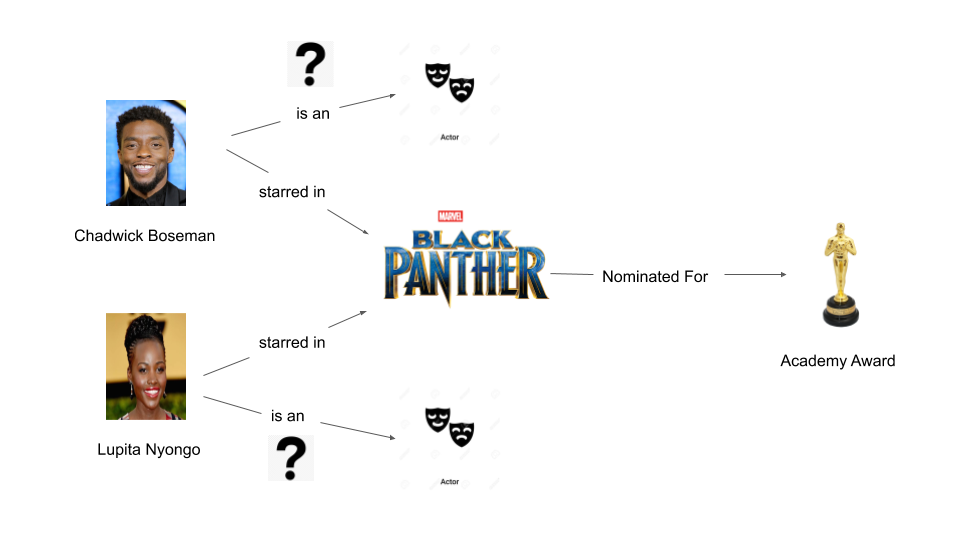
\includegraphics[width=\textwidth]{Objects_and_the_Relationships_Between_Them}
\end{figure}

\textbf{Challenges}. Reasoning about knowledge expressed in natural language ~\citep{minervini2019differentiable} is simple for humans, but trying to imitate this behaviour in computers reveals its underlying complexity. \newline 
The first task is providing a mechanism for perceiving syntax. Humans recognise text as sequences of words, and words as a sequence of characters. Characters can belong to different writing systems which can be dense - have a few characters used in a large number of combinations, or sparse - have a very large number of characters used in less combinations ~\citep{Hua2010}. A computer has to first be able to perceive these characters. \newline
The second task is even more challenging: semantics. Semantics is the meaning of words in language ~\citep{chomsky1955logical}. Semantics is what allows humans to understand each other in conversation, through written text, and through visual imagery. Semantics allow us to understand that an actor is a thing, and that things can have relationships with other things. Giving computers the capability to semantic understanding is very challenging because of the "messiness" of language. If a person is shown a word in the singular, and a word in the plural, for example "film" and "films" a person will most likely understand that there is not much difference in meaning between the two words, a computer may interpret them as having completely different meanings. Different words can also have similar meanings, for example "movie" and "film". Capturing this statistical similarity once again challenging for machines. And finally the order in which words are seen provides context, for example, the word "star" has completely different meaning in "Chadwick Boseman is a movie star" and "Black Panther looked up into the night sky an saw a star". \newline
The third task is organising information in such a way as to be able to reason about the knowledge it conveys. Humans build mental models using default reasoning ~\citep{reiter1980logic} - believing that most Objects A have relationship Relationship with Object B, with a small number of exceptions. For example we could believe that films (Object A) have not won (Relationship) an Oscar (Object B), except for films such as Black Panther (Object B). We will believe this is true for any given movie, unless we are familiar enough with movie history to identify the exceptions. Formallly, the default beliefs we hold are facts, and this process of reasoning allows us to infer new facts - plausible relationships between objects. In order to allow computers to use the same method of reasoning to perform inference, data has to be structured as facts and stored in a database ~\citep{angeli2013philosophers}. Computers are then capable of question answering given information within their database. The problem with this approach is facts are either present in the database or they are not i.e. questions can be answered exactly, or they cannot. There is no measure of plausibility that can be used to accept new potential facts, or discard implausible facts ~\citep{koller2007introduction}. \newline
\textbf{Encourging Progress}. The task of reasoning about knowledge expressed in natural language is a daunting one, however we have seen tremendous progress in statistical relational learning. The first major progress was the integration of the bilinear tensor product and neural networks ~\citep{socher2013reasoning}. This approach effectively extended linear tensor factorisation techniques to nonlinear tensor factorisation. The approach simultaneously introduced using pre-trained word embeddings to initialise entities and relations, instead of using randomly initialised word vectors. In this one approach, both reasoning and semantic representations were extended. \newline
The second time major progress was realised was with the use of complex valued embeddings for link prediction ~\citep{trouillon2016complex}. This approach extended the Bilinear Tensor product by making use of Hermitian dot product, the complex counterpart of the standard dot product between real vectors. The approach proposes complex vectors can effectively capture antisymmetric relations while retaining the efficiency benefits of the dot product. This was achieved by using representations with complex embeddings $\mathbb{C}$, allowing the model to capture the semantic meaning depending on the order of the embeddings. \newline 
The previous two milestones relied on shallow models that could scale to large datasets. Up until that point, research in link prediction had focused on minimising the parameterisation of models. Convolutional networks are parameter efficient models, and major progress was again realised with the use of convolutional deep learning models for link prediction ~\citep{dettmers2018convolutional}. The approach makes use of 2D embedding representations which allow the modelling of a high number of interactions between embeddings. \newline 
Despite this progress, we've yet to see this method knowledge-based reasoning deployed to real-life applications. Alternative methods such as approaches to solving the Stanford Question Answering Dataset (SQuAD) ~\citep{rajpurkar2016squad}, General Language Understanding Evaluation (GLUE) benchmarks ~\citep{liu2019roberta}, and the Alexa Prize ~\citep{ram2018conversational}, have seen greater commercial adoption. Applications of link prediction seem to be more focused on the evolution of relational databases, and have so far found utility in laboratory information management systems ~\citep{HARROW20192068}. \newline
\textbf{Remaining Challenges}. Perhaps the lack of adoption in link prediction is due to the current neural factorisation model state-of-the-art (SOTA) performance in open-domain question answering: 25.20\% ~\citep{balazevic2019hypernetwork}. A possible explanation for why SOTA performance is so low is that Toutanova and Chen ~\citep{toutanova2015observed} realised inverse relation test set leakage from the training set of FB15k. Because of this test set leakage, simple rule-based models were able to exploit inverse relations in the test set and achieve SOTA performance. Similarly, current neural factorisation model SOTA performance on the less challenging WN18RR dataset is 43.60\%. Dettmers et al. ~\citep{dettmers2018convolutional} created this dataset after discovering a similar test leakage problem in WN18. We can conclude that link prediction SOTA performance has to dramatically improve before wide-spread adoption can be realised.


%********************************** %Second Section  *************************************

\section{Modelling Techniques} %Section - 1.2

\subsection{Latent Feature Modelling} % Latent Feature Modelling
Entities and relations are words that can be represented as real-valued vectors [references]. These real-valued vectors form part of a euclidean embedding space that represents a knowledge domain [references]. The entity and relational vectors can be randomly generated, or be pre-computed to capture semantic meaning [references]. A classification model can then be constructed that generates a probability distribution over probable facts within the knowledge domain. In order to compute the probability distribution, a number of latent feature modelling techniques are used, including tensor factorisation [references], circular correlations [reference] and convolutional feature maps [reference]. These methods can broadly be defined as linear and nonlinear. Attractive attributes of linear latent models are their simplicity, ease of implementation and computational efficiency. Linear latent models however suffer from a lack of expressiveness and struggle to model complex, contradictory or incoherent relationships between entities. Nonlinear latent feature models are able to produce more expressive latent feature sets, and so more adept at capturing complex relationships. Nonlinear models however suffer from computational inefficiency and poorly generalise concepts. \newline
\subsection{Graph Feature Modelling} % Graphical Modelling
In Graph Feature Modelling, Knowledge Graphs (KG) are used to model domains. KGs are composed of nodes and edges, where nodes represent entities and edges represent relations. The graphical structure then captures local, quasi-local and global domain properties. This global structure exhibits particular properties about relations within the domain, characteristics of the entities of the domain, and local entity-relational sub-structures. These graph structure properties are used in supervised [reference] and unsupervised [Graph Infomax] settings for SRL tasks such as link prediction and entity-resolution. The directional nature of edges in graph structures (uni-relational and bi-relational) is also exploited to further enhance the fulfillment of SRL tasks [reference]. The assumption in general in KGs is that similar entities will be collocated within a local and quasi-local regions, and that global similiarty patterns between entities will be captured by the ensemble of all paths between entities. Link-based clustering [reference] is thus used at all these structural scopes, and supports link prediction and entity-resolution tasks. 
\subsection{Inductive Probabilistic Logic Programming}  % Inductive Probabilistic Logic Programming
Inductive logic programming uses ontological facts to discover new facts within a knowledge domain [reference]. logical rules check for things such as consistency. coherence and contradiction. Knowledge domains are implemented as knowledge bases (KB) that follow the resource description framework [reference]. KBs initialised in two steps: fact recording and materialisation - the discovery of new facts by running logical queries over the entire KB. KBs are extremely computationally demanding [reference], they also suffer from an inflexibility in modelling complex relationships due to their exactness, a fact is either true or false with no measure of ambiguity. Probabilistic logic programming languages have recently gained a lot of attention as flexible alternatives to logic programming languages as they are able to capture uncertainty in logical assertions through by modelling probability distributions over KB facts using stochastic variational inference. These models are thus more flexible in modelling complex relationships, and are also more computationally efficient [reference]. Inductive probabilistic logic programming has recently gained a lot of research attention due to it's capability of extending probabilistic logic programming languages with the capability of knowledge discovery. 

%********************************** % Third Section  *************************************
\section{Link Prediction with Latent Feature Models}  %Section - 1.3 
\label{section1.3}
\subsection{Knowledge Graph Latent Feature Models}
Link prediction with latent feature models involves building entity-relational representations from the nodes and edges of knowledge graphs expressed as subject-predicate object triples. These triples explicitly model facts within a knowledge domain. Entity and relational representations are commonly implemented as real-valued vectors. The vectors are then combined using compositional models, such as neural networks, to produce latent relational representations that can be used to compute the likelihood of plausible relationships between entities. The domain can be said to represent a multidimensiona embedding space into which the entities and relations are projected. Knowledge graph based latent feature modelling approaches are similar to semantic embedding representations [rerferenc]. They differ in that knowledge graph approaches explicitly model entity-relational interactions,  and semantic embedding approaches rely on the distributional word representation techniques [reference], relying on Skip-Gram [reference] and Contious Bag of Words [reference] to generate word representations. This is an implicit modelling of relationships between word vectors. \newline
\subsection{Factorisation of Latent Feature Models}
Factorisation attempts to model concepts between words, these facts are discovered using unsupervised techniques such as singular value decomposition. In the case of knowledge graphs, we obtain explicit representations of these concepts and can use them for entity-relational transformations that represent intermediate relational concepts that can then be used to determine plausible relationships when tested against subject entities.
Tensor factorisation is an approach used for link prediction with latent feature models. It involves modelling entity relationships as matrix slices that comprise a relational tensor. The entity between entities is then computed using a bilinlear tensor product [reference], where the inner product of the object entity is taken with the matrix relational representation before an inner product of the resultant representation is taken with the subject entity. Bilinear tensor factorisation models are efficient in their number of parameters but lack expressiveness. Multilayer perceptrons have been used to overcome the lack of expressiveness however often suffer from overfitting. Recently convolutional neural networks have been proposed to allow expressive factorisation [references], do not suffer from overfitting and remain computationally efficient. \newline
\subsection{Other of Latent Feature Modelling Approaches}
A number of alternative approaches to latent feature model factorisation have been proposed for link prediction, including circular correlation [reference], holographic entity-relational transformations [reference], toroidal representations [reference]. The rest of this dissertation focuses on factorisation of latent feature models, with the explicit representation of relational concepts. \newline

\nomenclature[z-DEM]{DEM}{Discrete Element Method}
\nomenclature[z-FEM]{FEM}{Finite Element Method}
\nomenclature[z-PFEM]{PFEM}{Particle Finite Element Method}
\nomenclature[z-FVM]{FVM}{Finite Volume Method}
\nomenclature[z-BEM]{BEM}{Boundary Element Method}
\nomenclature[z-MPM]{MPM}{Material Point Method}
\nomenclature[z-LBM]{LBM}{Lattice Boltzmann Method}
\nomenclature[z-MRT]{MRT}{Multi-Relaxation 
Time}
\nomenclature[z-RVE]{RVE}{Representative Elemental Volume}
\nomenclature[z-GPU]{GPU}{Graphics Processing Unit}
\nomenclature[z-SH]{SH}{Savage Hutter}
\nomenclature[z-CFD]{CFD}{Computational Fluid Dynamics}
\nomenclature[z-LES]{LES}{Large Eddy Simulation}
\nomenclature[z-FLOP]{FLOP}{Floating Point Operations}
\nomenclature[z-ALU]{ALU}{Arithmetic Logic Unit}
\nomenclature[z-FPU]{FPU}{Floating Point Unit}
\nomenclature[z-SM]{SM}{Streaming Multiprocessors}
\nomenclature[z-PCI]{PCI}{Peripheral Component Interconnect}
\nomenclature[z-CK]{CK}{Carman - Kozeny}
\nomenclature[z-CD]{CD}{Contact Dynamics}
\nomenclature[z-DNS]{DNS}{Direct Numerical Simulation}
\nomenclature[z-EFG]{EFG}{Element-Free Galerkin}
\nomenclature[z-PIC]{PIC}{Particle-in-cell}
\nomenclature[z-USF]{USF}{Update Stress First}
\nomenclature[z-USL]{USL}{Update Stress Last}
\nomenclature[s-crit]{crit}{Critical state}
\nomenclature[z-DKT]{DKT}{Draft Kiss Tumble}
\nomenclature[z-PPC]{PPC}{Particles per cell}
%!TEX root = ../thesis.tex
%*******************************************************************************
%****************************** Second Chapter *********************************
%*******************************************************************************

\chapter{Deep Learning}

\ifpdf
     \graphicspath{{Figs/Chapter2/}}
\else
    \graphicspath{{Chapter2/Figs/Vector/}{Chapter2/Figs/}}
\fi

There are many tasks which are hard to write algorithms for. For example, writing an algorithm the identifies a type of fruit using a picture of the fruit is a challenging undertaking. You could try to solve this problem by asking a number of yes or no questions which help whittle down the possibilities to a handful of fruit. A sensible question to ask might be - "Is the fruit round?". If the answer was yes, we could immediately discard options like strawberries, pineapples and pears. Another sensible question to ask might be - "Is the fruit orange?". If the answer is yes, again we could immediately discard unlikely candidates. Finally we could ask - "Is the fruit rough?". And if the answer was no, we could be pretty sure the picture we were looking at was an orange. \newline
The problem with this approach is that it is very brittle. You could ask a question that would lead a high likelihood that the image was indeed an orange, however the image may not in fact be an orange. For example apples could also be round, orange and smooth. More questions could try to disambiguate the two types of fruit, but there is enough variation in fruit that our algorithm could be confused. Writing rules in this way also is not scalable. There are a large number of types of fruits, and writing questions to determine each one quickly becomes intractable, let alone questions that help distinguish similar fruit. \newline 
Machine learning (ML) is used to solve such tasks, as well as others such as weather prediction, stock price forecasting and risk modelling ~\citep{hastie2009elements}. ML is the process of using data to build prediction models where these models typically output discrete (classification) or continuous (regression) values. ML uses a number of learning paradigms ~\citep{murphy2012machine}, including supervised learning, unsupervised learning and reinforcement learning, to train models. The models can be divided into three classes, namely shallow, deep and probabilistic ~\citep{hastie2009elements, murphy2012machine}. The models are trained using data to accomplish a task. \newline
\newpage
This chapter presents a discussion on the supervised learning paradigm, an analysis of the convolutional network ~\citep{lecun1998gradient} and recurrent network ~\citep{werbos1988generalization} deep learning models, and a discussion on deep learning training techniques, including dropout ~\citep{srivastava2014dropout} and batch normalisation ~\citep{ioffe2015batch} regularisation. 


%********************************** %First Section  **************************************

\section{Supervised Learning}

ML prediction models take as input a set of features. These features are attributes of a data sample. For example in the fruit prediction task mentioned above, input features would be the attributes of a fruit. They would include characteristics such as shape, colour, texture and size. These inputs are provided to a model that maps to outputs. In the example above, these outputs would be types of fruit, and could represent values such as oranges, apples, strawberries and pineapples, amongst others. The model is then taught (trained) to identify the correct fruit (output) based on the features (input) it receives. This type of training paradigm is called supervised learning \citep{bishop2006pattern, hastie2009elements, murphy2012machine}. \newline

\begin{figure}[H]
  	\caption{Supervised Learning}
   	\centering
    	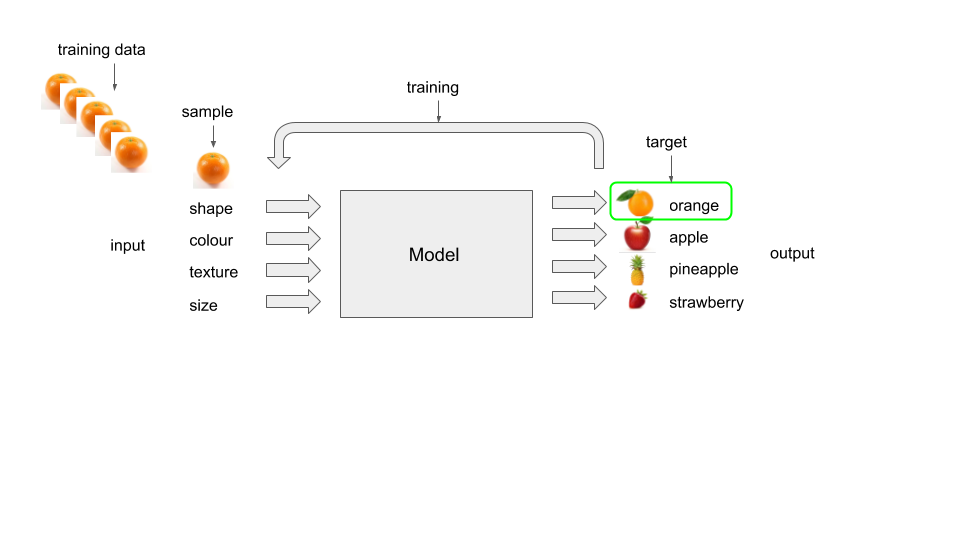
\includegraphics[width=\textwidth]{supervised_learning}
\end{figure}

Features can be continuous valued or discrete, where discrete values are referred to as categorical variables. Outputs can also be continuous or discrete, where discrete outputs are known as classes. Input-output pairs comprise a dataset which is represented as follows, \begin{math} D = \{(x_i, y_i)\}_{i=1}^N \end{math}, where \begin{math} D \end{math} is the dataset, \begin{math} x_i \end{math} is the input sample and \begin{math} y_i \end{math} is the output label. The model has to learn the correct mapping of input to output - features to label. We use data samples to train the model to recognise which features are correlated with which labels. The model is trained using an algorithm where it is shown a sample and it outputs what it believes is the correct label. If it gets the label wrong, an objective function is used to assess how large the error was, and the model is adjusted. We try to minimise this error during training, and because we try to minimise the objective function value, it is called a loss function. The algorithm is expressed as follows: \bigbreak

\begin{algorithm}[H]
	\SetAlgoLined
	\textbf{Input} 
	Training set \begin{math} D = \{(x_i, y_i)\}_{i=1}^N \end{math}, samples and labels\;
  	\begin{math} S_{batch} \gets sample(S, b) \end{math} // sample a minibatch of size \begin{math} b \end{math} \\
	 \For{(x, y) \begin{math} \in S_{batch} \end{math}}{
     		\begin{math} y \gets predict(x, y) \end{math} // predict label for sample \\
		\begin{math} e \gets y' - y \end{math} // compute error
     		}
	Update model w.r.t. \begin{math}  e \end{math}
	\caption{Supervised Learning}
\end{algorithm} \bigbreak

The model tries to build an approximation of the underlying distribution of data. Two important assumptions are made about the data, that the samples are independent and therefore order invariant, and that the data is identically distributed - that it is generated by the same underlying process for all samples. This type of data is called independently and identically distributed (IID) data. In the above example, the model will attempt to build decision boundaries around fruit classes given the features of the fruit. We can visualise this process in a 2-Dimensional setting using two fruit features, shape and colour. We generate a synthetic dataset using random number generation and then assign classes to our randomly generated classes, see Figure 4 below.

\begin{figure}[H]
  	\caption{Model Decision Boundary}
   	\centering
    	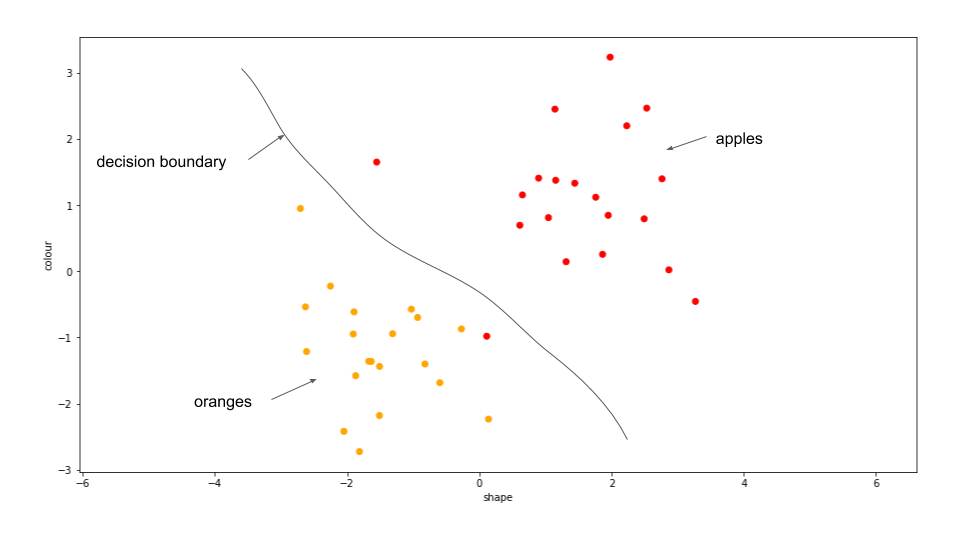
\includegraphics[width=0.8\textwidth]{oranges_and_apples_decision_boundary}
\end{figure}

Another class of data called non-IID data, where data samples are dependent and the sequence matters. These data are typically divided into training, validation and test sets for model training, where the type of data directly determines the best choice of model for mapping input to output. The choice of model also affects how the surface will look. A popular method of optimisation is gradient decent. Model updates are computed based on the first order parameter partial derivatives of the loss function.If the model only had three parameters, we could once again visualise how a possible loss surface might look. The job of the training algorithm, is to guide our model parameters toward a global minimum, in practice a local minimum is the best we can achieve.


%********************************** %Second Section  **************************************

\section{Deep Learning Models}

Deep learning models have become the preferred models for classification and regression tasks, and more broadly machine learning tasks. The reason for this is that deep models solve a major problem with shallow models - selecting the best features with which to represent samples ~\citep{Goodfellow-et-al-2016}. The problem of feature selection had resulted in a number of a methodology used during shallow model development: feature engineering. Feature engineering includes techniques such as bucketing, crossing, hashing and embedding ~\citep{murphy2012machine, Goodfellow-et-al-2016}. These techniques are designed to build sample representation that will result in high classification and regression accuracy. Deep models discovery optimal representations automatically, hence their superior performance on a number of machine learning tasks. \newline
Multilayer perceptrons (MLP) were the early deep learning models implemented as feed-forward neural networks consisting of $N$ layers, applied to an input vector $ x $. These models compute un-normalised scores known as logits, for each of the possible $ M $ outputs, classes and values in classification and regression respectively. They do this by executing a number of steps in an algorithm called the forward pass. Each step is called a layer, where an MLP can consist of a number of layers. A basic MLP consists of three of these layers, an input, hidden and output layer. The MLP computes a linear combinations of input features, then transforms the representation using a nonlinear hidden activation layer, before computing a linear combination of outputs. MLP models can be analytically defined as follows:

\begin{subequations}
\begin{gather}
	f_0 = x \\
	f_i=\sigma_i(W_if_{i - 1} + b_i) \quad i \in [1, N]
\end{gather}
\end{subequations}

where $f_0$ is the input layers, $f_i$ is the respective computation layer. Each layer has a particular number,  $m_i$, of neurons. The parameters of a layer consist of a matrix $W_i \in \mathbb{R}^{m_i \times m_{i-1}}$ and bias vector $b_i \in  \mathbb{R}^{m_i}$. Each layer also has a non-linear activation function $\sigma_i$. \newline
Loss functions are used to train deep models under a supervised learning paradigm. The error computed by the loss is used in a process called back propagation - the computing of parametric first order partial derivatives, and the adjustment of the parameters in direction and magnitude of their respective derivative. This process is formally described by:

\begin{subequations}
\begin{gather}
	\frac{\partial E} {\partial W_n} = \frac{\partial F} {\partial W}(W_n, X_{n-1})\frac{\partial E} {\partial X_n} \\
	\frac{\partial E} {\partial X_{n-1}} = \frac{\partial F} {\partial X}(W_n, X_{n-1})\frac{\partial E} {\partial X_n} 
\end{gather}
\end{subequations}

where $\frac{\partial F} {\partial W}(W_n, X_{n-1})$ is the Jacobian of $F$ with respect to $W$ evaluated at the point $(W_n, X_{n-1})$, and  $\frac{\partial F} {\partial X}(W_n, X_{n-1})$ is the Jacobian of $F$ with respect to $X$. The Jacobian of a vector function is a matrix containing the partial derivatives of all the outputs with respect to all the inputs. Together the forward pass algorithm and back propagation, allow the automatic discovery of the most meaningful representation to compute the model output. We refer the reader to ~\citep{Goodfellow-et-al-2016} for a review on loss functions, as well as a more detailed discussion on the forward pass and back propagation. 

\subsection{Convolutional Networks}

MLPs suffer from an explosion of parameters  ~\citep{krizhevsky2012imagenet}. In fact when modelling a sample using a regular feed-forward network, we find that the number of model parameters grows exponentially. For example, a feed-forward network with $2$ hidden layers consisting of $512$ and $256$ neurons respectively, an output size of $10$ and an input sample shape of $\left [ \begin{matrix} 200 & 1 \end{matrix} \right] $, then the model ends up having: 

\begin{equation}
	parameters = (200 \times 512 + 512) + (512 \times 256 + 256) + (256 \times 10 + 10)
\end{equation}

a total of $236,810$ parameters. Compounding this issue, is the incapability of MLPs to take advantage of structure in data, thus having no way of compensating for distributions of representations of the same conceptual sample. In order to cater for sample representation distribution variance, MLPs have to be larger, so as to have enough learning capacity to be able to hold sufficiently representative feature mappings ~\citep{lecun1998gradient}. \newline
Convolutional neural networks (CNN) have been developed to overcome both the above mentioned problems experienced by MLPs. CNNs make use of the convolutional operation during representation learning. This operation allows CNNs to achieve representation translation and location invariance ~\citep{simonyan2014very}. Translation invariance allows the CNN to build an object representation that is consistent under transformation, for example an image rotation would lead to a consistent final sample representation being generated. Locality invariance allows the model to generate the same representation a sample concept if the concept signal shifts along the dimensions of the representation. These properties allow CNNs to model the true distribution of samples using fewer parameters and smaller datasets. In the following we discuss the CNN forward pass algorithm. \newline
\textbf{Convolutional Layers.} CNNs perform a convolutional operation on a sample using a trainable representation filter. The operation constructs latent features of the sample by generating a feature map representation. Every filter is N-dimensional, for example 2-dimensional, and small spatially (along width and height), but extends through the full depth of the input, where the input itself can also be N-dimensional, producing an input volume.  During the forward pass, each filter is convolved across the width and height of the input volume where the element-wise dot product is computed between the entries of the filter and the input at any position. A 2-dimensional activation map is generated as a result, that gives the responses of that filter at every spatial position. Every convolutional layer has a set of corresponding filters, and each of them produce separate 2-dimensional activation maps. Each feature map is then stacked along the depth-dimension to produce an output volume. The convolution operation is described by:

\begin{subequations}
\begin{gather}
	\frac{\partial E} {\partial W_n} = \frac{\partial F} {\partial W}(W_n, X_{n-1})\frac{\partial E} {\partial X_n} \\
	\frac{\partial E} {\partial X_{n-1}} = \frac{\partial F} {\partial X}(W_n, X_{n-1})\frac{\partial E} {\partial X_n} 
\end{gather}
\end{subequations}

% spatial and depth-wise convolutions
It is possible to decompose convolution operations into spatial and depth-wise convolutions \cite{reference}. A spatial convolution operates on different regions of an image, producing distinct representations for each region, for example and image can be divided into four regions, where a spatial convolution operates independently on each of these regions using region-specific filters.This operation produces four distinct feature maps which are later flattened into a single hidden layer representation, before begin run through a linear layer to generate the final logits. In a depth-wise convolution, the distinct convolutional feature maps are generated using the depth dimensions of the input image, typically three dimensions with images, the red, blue and green image channels in a colour image. Channel-specific filters are used to generate these feature maps and once again the future maps are flattened prior to computing logits for the model classes. \newline


%********************************** %Third Section  **************************************

\section{Regularisation}

%Deep Learning Best Practice}
 % initialisation e.g. xavier initialisation and truncated normal
 Xavier initilisation \cite{reference} is commonly used to initialise model parameters. This initialisation technique has the benefit of non-bias. It also influences the starting position on the loss surface increasing the likelihood of convergence. An other common parameter initialisation strategy is truncated normal initialisation \cite{reference}, where model paramaters are sampled from a univariate Gaussian distribution with mean zero and variance one. \newline
 % optimiser
The Adam \cite{reference} optimiser is commonly used for model training. This optimiser is an adaptive moment optimiser that scales the learning rate depending on the scale of parameter update changes. Other optimisers used for parameter updates include stochastic gradient descent \cite{reference}, ADAG-Grad \cite {reference} and RMS-Prop \cite{reference}. \newline
% learning rate scheduling
Learning rate scheduling \cite{reference}, the practice of reducing the learning rate after successive training cycles is now also common. It is implemented either as a continual process, where the learning rate is reduced by some proportion after every iteration, or on a step basis, where the learning rate is reduced by a proportion after every epoch. \newline
 % Hyperparameter optimistaion 
One of the most challenging aspects of model training is hyper parameter optimistaion \cite{reference}. Bayesian optimisation techniques have been used recently to overcome this problem \cite{reference}. Another hyper parameter search technique commonly used is random grid search \cite{reference}. This technique relies on iterations of hyper parameter sets that are uniformly sampled from range of available values. \newline

Model over parameterisation can lead to overfitting. This because the degrees of freedom available to estimate a function allow very complex nonlinear functions to be discovered, where these nonlinear functions or not representative of the generative process of the data at all \cite{reference}. These overfitting makes the model very sensitive to the training data, and results in poor generalisation across training, validation and testing data. This problem forms part of the broader bias/variance trade off, specifically high model variance due to over parameterisation. Deep learning models are particularly sensitive to overfitting given the high number of parameters present within the model. In order to compensate for this overfitting, it is common zero out a sample of neurons within a deep learning network. This has the effect of removing partial dependence between nodes deeper within the network, a form of principal component analysis generating independent latent features. These latent features result in a simpler model representation of the generative process of the data, and therefore allow it to generalise better across datasets. \newline

Batch normalisation attempts to account for internal covariance shift \cite{reference}. Batch normalisation is inspired from population based feature mean normalisation, when the entire population is taken into consideration when computing the mean and standard deviation of the values which the feature can take on within the dataset. When training a deep learning model, it is common to perform a uniform random shuffle of the training set, then subdivide that the set into mini-batches \cite{reference}. This is the same process of taking a uniform random sample batch from the training data. The size of the sample batch determines whether the normalised features remain within distributional alignment of the population. In order to compensate for the resultant loss computed after a foward pass, it is important to re-align feature vector parameters to the sample distribution mean and standard deviation estimators. The generated loss surface is thus a closer approximation to the true loss surface of the population, and subsequent parameter updates do not suffer from sample distributional distortion. This results in improved test accuracy as the model is able to more closely approximate the true distribution of the data. \newline 

\subsection{Loss Surface Analysis}
Defining an objective function is best informed by analysing the surface it generates. If the objective functions aims to minimise an error, it is a loss function, and if an objective function maximises an expected return, it is a reward function. Nonlinear factorisation models are commonly trained using loss functions presented in the following table:

\begin{table}[H]
	\centering
	\begin{tabular}{lllllllllll}
  		\textbf{Name} & \textbf{Expression} \\
  		\hline
  		Log (Nickel, Tresp, and Kriegel 2011) & $e^T_1W_r e_2$  \\
  		Constrastive Max Margin (Bordes et al. 2013) & $|| e_1 + w_r - e_2 ||$ \\
  		Cross Entropy (Socher et al. 2013) & $u^T_r f(e_1W_r^{[1..k]} e_2 + V_r \begin{bmatrix}e_1 \\ e_2\end{bmatrix} + b_r)$ \\
  		Binary Cross Entropy (Nickel, Rosasco, and Poggio 2016) & $r^T_p(e_s * e_o)$ \\
  		Softmax Cross Entropy (Balazevicl, Allen, and Hospedales 2018) & $f(vec(e_1 * vec^{-1}(w_rH))W)e_2$ \\
  		Sparse Categorical Cross Entropy (Magangane and Brink 2019) & $f(vec(e_1 * vec^{-1}(w_rH))W)f(vec(e_2 * vec^{-1}(w_rH))W)$
		\end{tabular}
 	\caption {Scoring functions of link prediction models. $*$ is the convolutional operator $F_r = vec^{-1}(w_rH)$ the matrix of relation specific convolutional filters, $f$ is a non-linear function}
\end{table} 

% loss function choice
The choice of loss function determines the training loss surface which in turn determines the expected model accuracy and convergence rate.


%%!TEX root = ../thesis.tex
%*******************************************************************************
%****************************** Third Chapter **********************************
%*******************************************************************************
\chapter{Neural Tensor Factorisation}

% **************************** Define Graphics Path **************************

\ifpdf
    \graphicspath{{Chapter3/Figs/Raster/}{Chapter3/Figs/PDF/}{Chapter3/Figs/}}
\else
    \graphicspath{{Chapter3/Figs/Vector/}{Chapter3/Figs/}}
\fi


Open domain question answering is an area of research concerned with reasoning about knowledge expressed in natural language. Knowledge base (KB) link prediction using latent feature modelling is an approach that has been applied to this task, with varying degrees of success  ~\citep{nguyen2017novel, diefenbach2018wdaqua, kristiadi2019incorporating}. This approach aims to rank plausible relationships between entities by using using trainable embedding representaitons. Previous latent feature models have focused on limiting the number of parameters so as to be able to scale to large KBs, at a cost of complex entity-relational interaction modelling. \newline
Neural tensor networks (NTN), An extension to tensor factorisation was the first successful approach at taking advantage of expressiveness of deep models. It relied on adding a recursive network (RCN) representation to the bilnear tensor product, and wrapping that representation in a fully connected layer to then compute a relational score. Convolutional entity representations (ConvE) were similarly effective at extending tensor factorisation approaches by applying the convolutional operation in modelling entity-relational interactions, before completing a factorisation to compute a relational score. Hypernetworks were then applied to the ConvE model (HypER) to add further expressive power by pre-computing relational filter representations for subsequent use in a neural tensor factorisation. \newline
In this chapter we examine the NTN model, and attempt a simple improvement by applying Adam optimisation and hyperparameter random search to the training algorithm. We then introduce HypER+, an extension to the HypER model which compensates covariate shift introduced by augmenting relational filters with a hypernetwork. We then extend HypER+ to make use of pre-trained GloVe word embeddings, and address the problem of entity interaction sparsity in KBs.


% **************************** Section 1 **************************

\section{Neural Tensor Networks}

\subsection{Neural Tensor Factorisation}
RESCAL introduced the bilinear tensor product for relational scoring ~\citep{nickel2011three}. This model makes use of entity vectors and a relational tensor, where each relation type is modelled as a matrix slice of the tensor. RESCAL is defined as follows:

\begin{equation}
	f_{i, j, k}^{RESCAL} := e_i^TW_ke_j = \sum_{a=1}^{H_e}\sum_{b=1}^{H_e}w_{a,b,k}e_{ia}e_{jb}
\end{equation}

where $f$ is the relational score, $e_i$ is the subject, $e_j$ is the object, and $W$ is the relational tensor. This model linearly models entity-relational interactions by using the dot product operator to construct a latent subject-relation representaiton, before computing a relational score using the dot product operator between the subject-relational representation and the object. RESCAL is thus a linear factorisation composition. \newline
A natural extension to this method is to include a nonlinearity for entity-relational interaction modelling. This extension was introduced by (Jenatton et al. 2012) ~\citep{jenatton2012latent}.This model uses as sigmoid nonlinearity to compute a probability of relational plausibility from the relational score computed using the bilinear tensor product. The model is defined as follows:

\begin{subequations}
	\begin{gather}
		n_{ik}^{j} = e_i^TW_ke_j \\
		\sigma(t) = \frac{1}{1 + e^-t} \\
		\mathbb{P}\left [ R_j(S_i, O_k) = 1 \right ] = \sigma(n_{ik}^{j})
	\end{gather}
\end{subequations}

where $n$ is the relational score, $\sigma$ is the sigmoid function, a value in the range $\in \left ( 0, 1 \right ]$, and $\mathbb{P}$ is the probability of relational plausibility between $S$ and $O$ indexed by relation $R$. This model introduces non-linear entity-relational interaction modelling to tensor factorisation. 

\subsection{Recursive Neural Tensor Factorisation}
Socher and Chen et al (2013) extend nonlinear tensor factorisation by introducing recursive entity representations in the composition of the relational score ~\citep{socher2013reasoning}. Recursive networks (RCN) try to capture the rules for word combinations by constructing compositional representations of two words ~\citep{socher2012semantic}. The NTN model tries to take advantage of these compositional rules by adding them to the bilinear tensor product and augmenting the nonlinear tensor factorisation. The RCN extended nonlinear tensor factorisation model is defined as follows:

\begin{equation}
	g(e_1, R, e_2) =  u_R^Tf(e_1^TW_R^{\left [1:k\right ]}e_2 + V_R\left [ \begin{matrix} e_1 \\ e_2 \end{matrix} \right ] + b_R)
\end{equation}

where $g$ is the relational score, $f$ is the hyperbolic sigmoid function, a value in the range $\in \left [ -1, 1 \right ]$, $e_1^TW_R^{\left [1:k\right ]}e_2 $ is the bilinear tensor product, $V_R\left [ \begin{matrix} e_1 \\ e_2 \end{matrix} \right ]$ is the recursive composition of the subject and object, and $b$ is the bias. \newline

The contrastive max-margin objective is minimised during training. This objective computes a confidence magnitude on a true correct sample - a fact present in the KB, and a confidence magnitude on a corrupt sample - a randomly generated fact not present in the KB. The correct and corrupt samples are used by the objective as follows:

\begin{equation}
	J(\si{\ohm}) =  \sum_{i=1}^N\sum_{c=1}^Cmax(0,1 - g(T^{(i)}) + g(T_c^{(i)})) + \lambda\left\lVert \si{\ohm} \right\rVert_2^2
\end{equation}

where $J$ is the loss value, $\si{\ohm}$ are the model trainable parameters $u, W, V, b, and E$, $N$ is the number of training triplets, $C$ is the number of randomly corrupted facts. $g(T^{(i)}$ is the confidence in the true fact computed by the model, and $ g(T_c^{(i)}$ is the confidence in the corrupt fact computed by the model. Finally $\lambda\left\lVert \si{\ohm} \right\rVert_2^2$ is the ridge ($L_2$) regression regulariser. \bigskip

The NTN model training algorithm also makes use of pre-trained word vectors developed by (Turian et al. 2010) ~\citep{turian2010word}. These are 100-dimensional embeddings, which are aggregated by the set of words that represent an entity. For example for the entity \textit{homo sapien}, the resulting word representation is $V_{homo \; sapiens} = 0.5(V_{homo} + V_{sapien})$. These word vectors are trainable, and updated during back propagation, producing a distributed word representation that aligns with the KB.

\subsection{Modern Optimisation}

Deep model training loops can suffer from noise such as data subsampling, and regularisation techniques such as ridge regression and dropout. Adaptive moment estimation (Adam) is a first order gradient-based stochastic optimisation algorithm that compensates for this this noise ~\citep{kingma2014adam}. Adam computes the first and second order gradients of the loss and add them to the loss, combining the advantages of AdaGrad ~\citep{duchi2011adaptive} and RMSprop ~\citep{tieleman2012lecture}. Adam efficiently regulates parameter update magnitude size, accelerating toward local optima and remaining small in sparse regions. \newpage
Setting model hyperparameters remains a challenge in deep model training. A simple method proposed to address this problem is hyperparameter random search ~\citep{bergstra2012random}. This approach improves on grid search by matching or exceeding model performance in a fraction of the compute time. Hyperparameter random search takes advantage of the fact that for most datasets only a subset of the hyperparameters contribute meaningful variance in model performance, eliminating the need for an exhaustive brute force search over a large combinatorial search space.

\subsection{Training Algorithm}

(Doss et al. 2015) reimplement the NTN model in Tensorflow ~\citep{abadi2016tensorflow}. This model severely under performs the original model, relying on AdaGrad optmisation and the same hyperparaemeters. We apply Adam optimsation as well as hyperparameter optimisation using random search, in attempt to improve its performance. The new training algorithm is as follows: \bigbreak

\begin{algorithm}[H]
	\textbf{loop} // repeat for $N$ experiments using random uniform hyperparameter configuration \\
		\SetAlgoLined
		\textbf{Input} 
		Training set \begin{math} D = \{(x_i, y_i)\}_{i=1}^N \end{math}, samples and labels\;
  		\begin{math} S_{batch} \gets sample(S, b) \end{math} // sample a minibatch of size \begin{math} b \end{math} \\
	 	\For{(x, y) \begin{math} \in S_{batch} \end{math}}{
     			\begin{math} y_{correct} \gets predict(x, \; y_{correct}) \end{math} // predict label for sample \\
			\begin{math} y_{corrupt} \gets predict(x, \; y_{corrupt}) \end{math} // predict label for sample \\
			\begin{math} e \gets contrast(y_{correct}, \; y_{corrupt}) \end{math} // compute error
     			}
		Update model w.r.t. \begin{math}  e \end{math} // using Adam optimser \\
	\textbf{end loop}
	\caption{Updated NTN Training Algorithm}
\end{algorithm} \newpage


% **************************** Section 2 **************************

\section{Hypernetwork Tensor Factorisation}

\subsection{Convolutional Tensor Factorisation}
ConvE introduced the convolutional operator to link prediction model composition ~\citep{dettmers2018convolutional}. Specifically, this operator increases expressiveness in subject-predicate interaction modelling by using 2-dimensional instead of 1-dimensional convolutions, being particularly effective at modelling knowledge graph (KG) nodes with high indegree. ConvE concatenates subject and predicate vectors, creating a 2-dimensional representation. Convolutional filters are then applied to this representation before it is flattened by a fully connected layer. The dot product of this generated representation is then taken with the object vector, producing a measure of confidence in the relation, before a logistic sigmoid is applied to compute a probability of plausibility. The model is defined as follows:

\begin{equation}
	\psi_r(e_s, \; e_o) = g(vec(f(\left [ \overline{e_s}; \overline{r_r} \right ]*w))W)e_o
\end{equation}

where $\psi_r$ is the relational score, $e_s$ is the subject, $e_r$ is the object, and $r_r$ is the predicate. $f$ is the concatenation operation between the subject and predicate, $w$ are the 2-dimensional convolutional filters and $W$ is the parameterised matrix of the fully connected layer. $g$ is a ReLU non-linearity applied to the fully connected layer output. ConvE is thus a convolutional factorisation composition. The computed relational probability is defined as follows: 

\begin{equation}
	p = \sigma(\psi_r(e_s,e_o)) 
\end{equation}

The binary cross-entropy objective is minimised during training. This objective is particularly effective as during we expect only a single true class during inference, modelled as $1$, and every other class to be false, $0$. The objective is defined follows:

\begin{equation}
	L(p, \; t) =  -\frac{1}{N}\sum_i(t \cdot log(p_i) + (1 - t_i) \cdot log(1 - p_i))
\end{equation}

where $L$ is the loss value, $p$ is the relational probability computed by the model, and $t$ is the target. $N$ is the number of entities, and $i$ is the batch sample number. \newpage


\subsection{Hypernetwork Tensor Factorisation}

Hypernetworks are meta networks that generate parameters for a main network ~\citep{ha2016hypernetworks}. The networks essentially index the parameters of a main network as a configuration given input. This input is typically in the form of an embedding vector that describes the entire weights of a given layer. This configuration is learned given a scenario experienced by the main network, for example when performing sequence prediction, it may be advantageous for the main network to change its behaviour (parameter configuration) depending on the sequence window. The hypernetwoirk model can be defined as follows: 

\begin{equation}
	K^j = g(z^j), \quad \forall j = 1, \dots, D
\end{equation}

where $K$ are the layer parameters, $g$ is the hypernetwork composition, and $z$ is the hypernetwork input. \bigskip

HypER is inspired by ConvE, and implements a convolutional operator that models entity-relational interactions ~\citep{balazevic2019hypernetwork}. HypER makes use of a hypernetwork to generate relation-specific convolutional filter. The subject and relational-filter are then used in a convolution operation to generate latent representation which is then flattened by a fully connected layer. The dot product of this generated representation is then taken with the object vector, producing a measure of confidence in the relation, before a logistic sigmoid is applied to compute a probability of plausibility. The model is defined as follows: 

\begin{equation}
	\phi_r(e_1, \; e_2) = f(vec(e_1 * (vec^{-1}(w_rH)))W)e_2
\end{equation}

where $\phi_r$ is the relational score, $e_1$ is the subject, and $e_2$ is the object. $vec^{-1}$ is the transformation that reshapes the output of the hypernetwork into a set of relation-specific convolutional filters, $w$ is the predicate input and $H$ is the parameterised matrix of the fully connected layer of the hypernetwork. $f$ is a ReLU non-linearity applied to the fully connected layer output of the main network. HypER is thus a hypernetwork factorisation composition. The computed relational probability is defined as follows: 

\begin{equation}
	p = \sigma(\phi_r(e_1,e_2)) 
\end{equation}

The HypER training algorithm minimises the binary cross-entropy objective. \newpage

\textbf{Hyper Covariate Shift}. We make the observation that hypernetworks may also suffer from covariate shift. The network parameters are adjusted during training, resulting in a distributional drift across the entire main network as training progresses. To address this problem, we introduce batch normalisation between the hypernetwork and main network. We adjust the model accordingly, and introduce HypER+. \bigskip 

\textbf{Training Algorithm}. HypER+ is trained using the binary cross-entropy objective. We use the same hyperparameters as the original HypER model, as well as the Adam optimiser. The HypER+ training algorithm is as follows: \newline

\begin{algorithm}[H]
	\SetAlgoLined
	\textbf{Input} 
	Training set \begin{math} D = \{(x_i, y_i)\}_{i=1}^N \end{math}, samples and labels\;
  	\begin{math} S_{batch} \gets sample(S, b) \end{math} // sample a minibatch of size \begin{math} b \end{math} \\
	 \For{(x, y) \begin{math} \in S_{batch} \end{math}}{
     		\begin{math} y' \gets predict(x, \; y') \end{math} // predict label for sample \\
		\begin{math} e \gets y' - y \end{math} // compute error
     		}
	Update model w.r.t. \begin{math}  e \end{math} // using Adam optimser \\
	\caption{HypER+ Training Algorithm}
\end{algorithm} \bigbreak

%%!TEX root = ../thesis.tex
%*******************************************************************************
%*********************************** Fourth Chapter *****************************
%*******************************************************************************


\chapter{Results and analysis}  %Title of the Fourth Chapter

\ifpdf
     \graphicspath{{Figs/Chapter4/}}
\else
    \graphicspath{{Chapter4/Figs/Vector/}{Chapter4/Figs/}}
\fi

This chapter examines the three hypotheses of this study, including the application of training algorithm optimisations to recursive neural tensor networks (NTNs), compensating for covariate shift introduced by hypernetworks during convolutional tensor factorisation, and finally the initialisation of entity and relation embeddings using pre-trained word vectors. 


%********************************** %Recursive Neural Tensor Networks  **************************************

\section{Recursive neural tensor networks}

\subsection{Datasets} 

For the first set of experiments we use the WordNet \unskip ~\citep{miller1995wordnet} and Freebase \unskip ~\citep{bollacker2008freebase} link prediction benchmark datasets.\ WordNet is a lexical database for English, and a taxonomy with hypernym relationships ("is a") and synonym sets. Freebase is a large collaborative knowledge base consisting of data about the world, composed mainly by community members. It is an online collection of structured data harvested from many sources, including user-submitted wiki contributions. The WordNet dataset contains a total of 136,611 triples, and Freebase a total of 375,499 triples. Visualisations of the respective knowledge graphs (KGs), as well as a sample of resource description framework (RDF) triple encoded facts, are presented in Figures 4.1 to 4.4. KG summary statistics are presented in Figures 4.5 to 4.7, and Table 4.1.

\begin{figure}
   	\centering
    	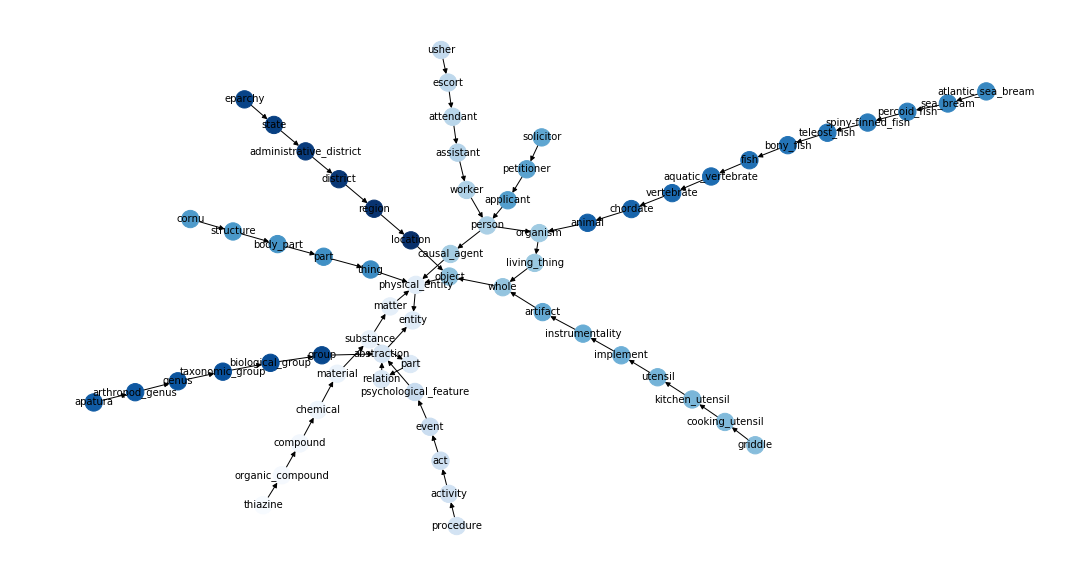
\includegraphics[width=0.9\textwidth, height=0.5\textwidth]{Wordnet}
	\captionsetup{justification=centering}
	\caption{A subset of WordNet facts structured as a KG. Entities are nodes, and relations are edges, where facts are encoded as RDF triples.}
\end{figure}

\begin{figure}
   	\centering
    	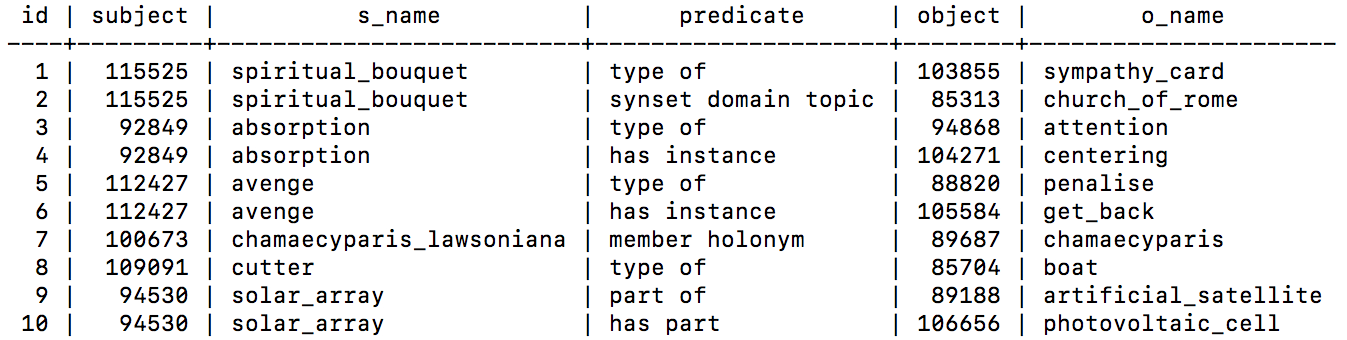
\includegraphics[width=0.9\textwidth, height=0.2\textwidth]{wordnet_fact_sample}
	\captionsetup{justification=centering}
	\caption{A sample of RDF triples from the WordNet KG.}
\end{figure}

\begin{figure}[H]
   	\centering
    	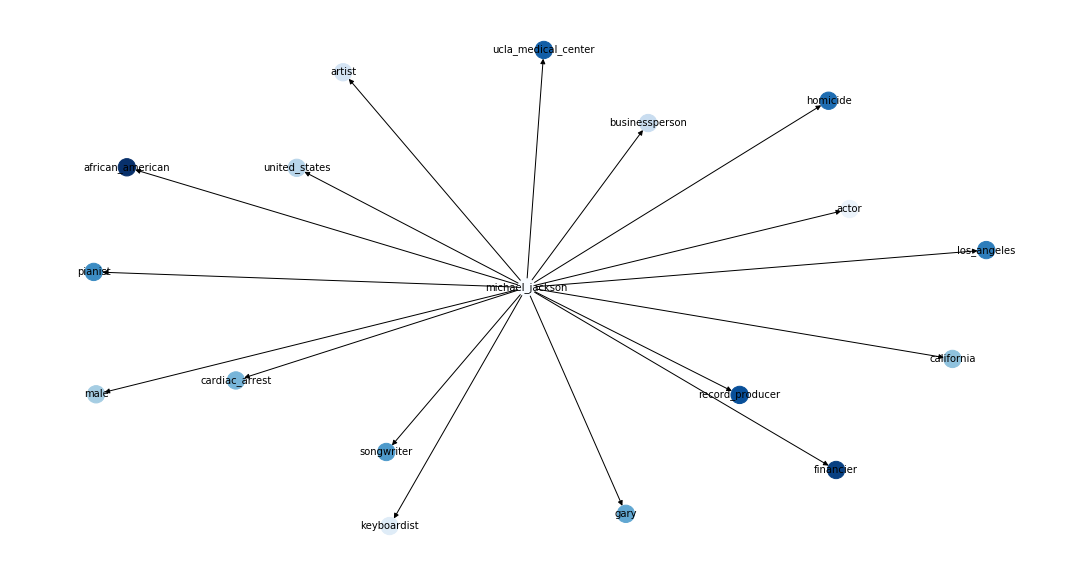
\includegraphics[width=0.9\textwidth, height=0.5\textwidth]{Freebase}
	\captionsetup{justification=centering}
	\caption{A subset of Freebase facts structured as a KG. Due to the size of Freebase, only a subset of facts related to the subject "Michael Jackson" is presented.}
\end{figure}

\bigskip
\bigskip
\bigskip
\bigskip

\begin{figure}[H]
   	\centering
    	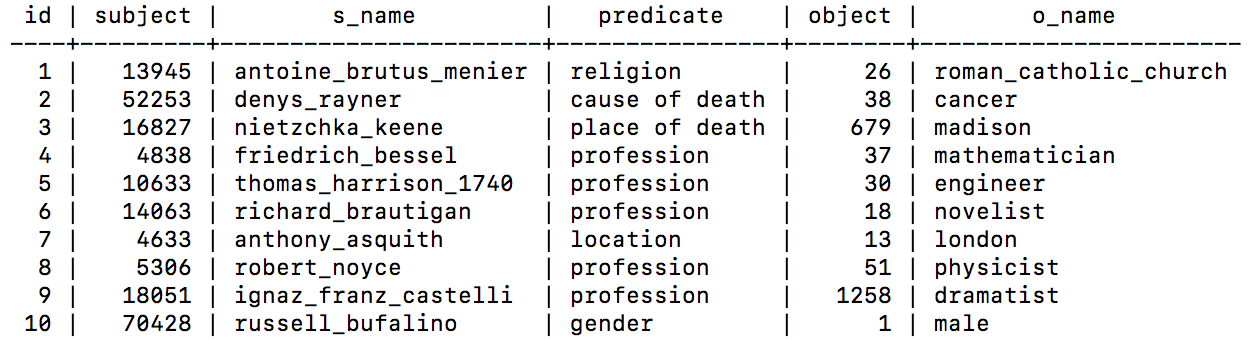
\includegraphics[width=0.9\textwidth, height=0.2\textwidth]{freebase_fact_sample}
	\captionsetup{justification=centering}
	\caption{A sample of RDF triples from the Freebase KG.}
\end{figure}

\noindent WordNet is comprised of a set of relation types including similar, opposite, subordinate, part, and entailment. Freebase is comprised of an open-ended collection of relation types, including symmetric, asymmetric, transitive, composition, hierarchy, reflexive, irreflexive and inversion. Freebase also contains more entities, relations between entities, and facts, than WordNet. 


%********************************** %Subject **************************************

\begin{figure}
	\begin{subfigure}[b]{.5\linewidth}
   		\centering
    		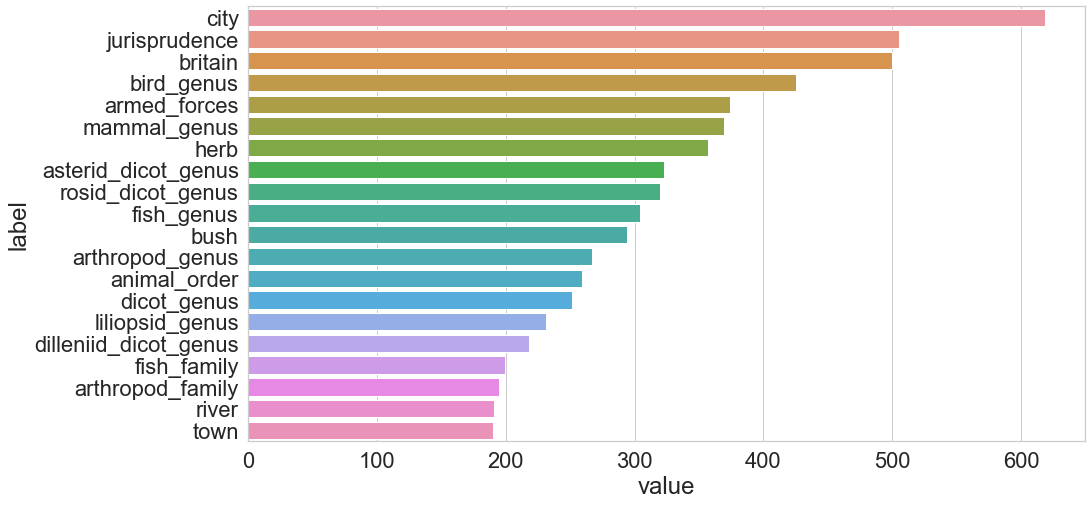
\includegraphics[width=1.0\linewidth, height=0.6\linewidth]{Wordnet_Subject_Counts}
		\captionsetup{justification=centering}
		\caption{WordNet}
	\end{subfigure}
	\begin{subfigure}[b]{.5\linewidth}
   		\centering
		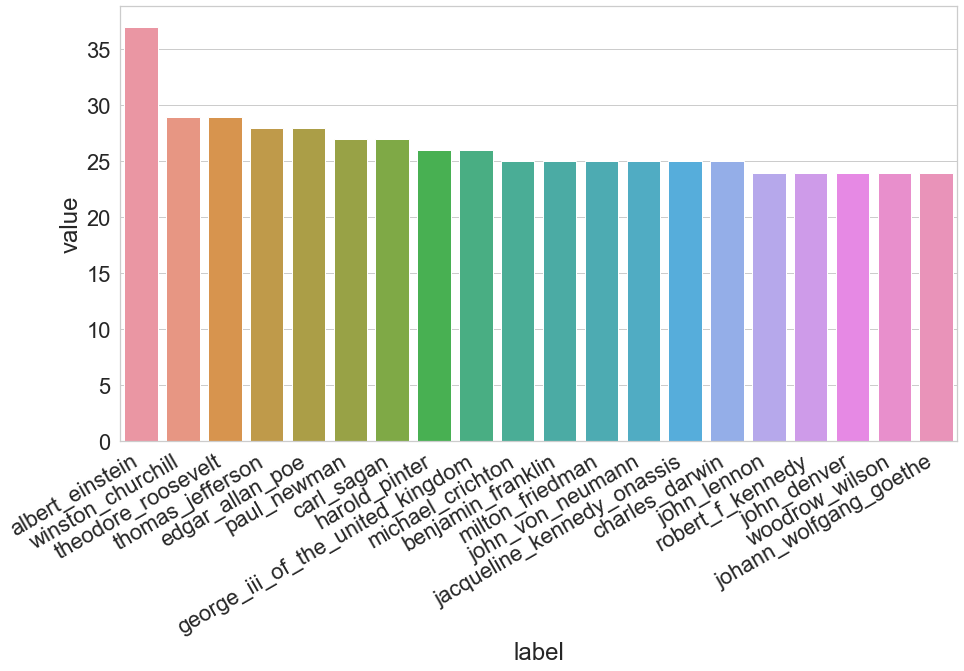
\includegraphics[width=1.0\linewidth, height=0.6\linewidth]{Freebase_Subject_Counts}
		\captionsetup{justification=centering}
		\caption{Freebase}
	\end{subfigure}
	\captionsetup{justification=centering}
	\caption{Histogram showing the number of times the 20 most frequent subject labels occur in KG facts, in the WordNet and Freebase link prediction datasets.}
\end{figure}


%********************************** %Predicate  **************************************


\begin{figure}
	\begin{subfigure}[b]{.5\linewidth}
   		\centering
    		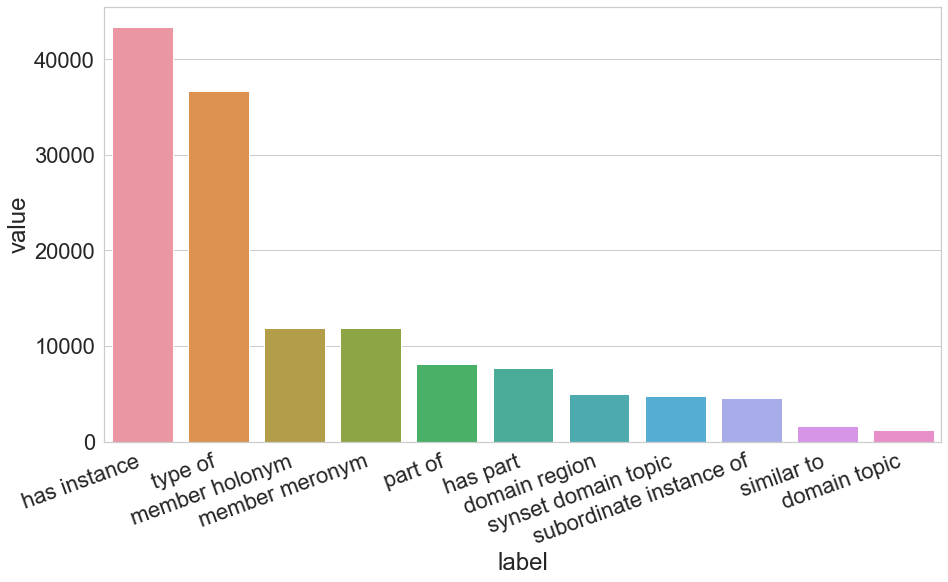
\includegraphics[width=1.0\linewidth, height=0.6\linewidth]{Wordnet_Predicate_Counts}
		\captionsetup{justification=centering}
		\caption{WordNet}
	\end{subfigure}
	\begin{subfigure}[b]{.5\linewidth}
   		\centering
		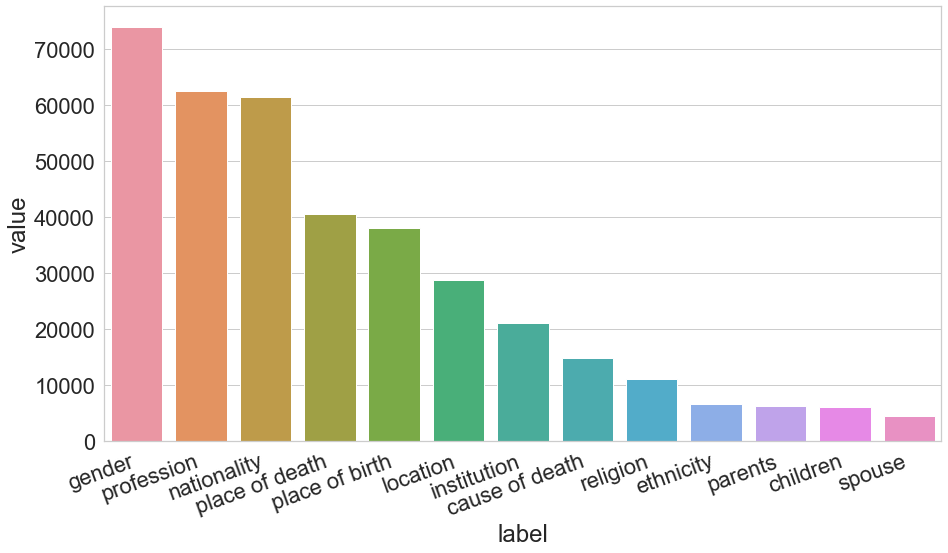
\includegraphics[width=1.0\linewidth, height=0.6\linewidth]{Freebase_Predicate_Counts}
		\captionsetup{justification=centering}
		\caption{Freebase}
	\end{subfigure}
	\captionsetup{justification=centering}
	\caption{Histogram showing the number of times predicate labels occur in KG facts, in the WordNet and Freebase link prediction datasets.}
\end{figure}


%********************************** %Object  **************************************

\begin{figure}
	\begin{subfigure}[b]{.5\linewidth}
   		\centering
    		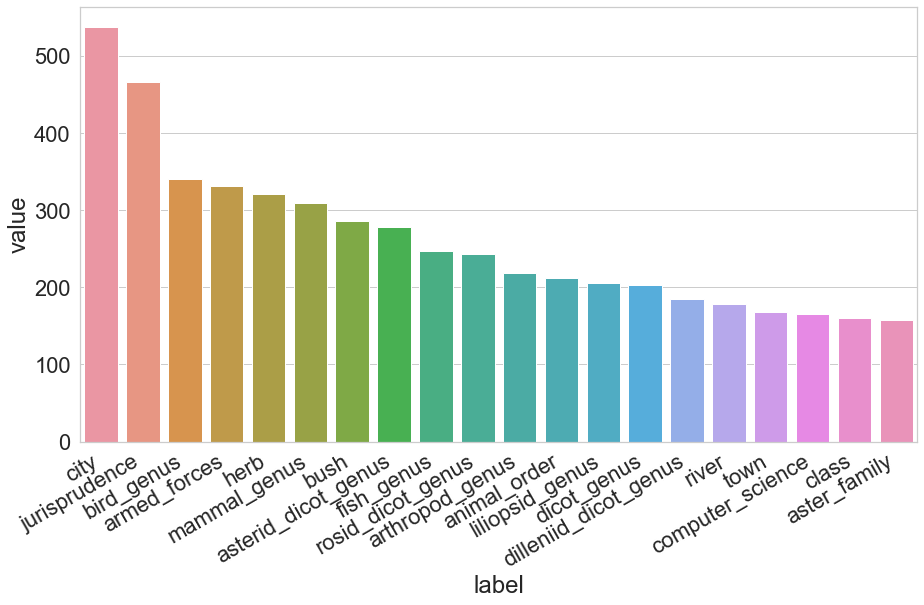
\includegraphics[width=1.0\linewidth, height=0.6\linewidth]{Wordnet_Object_Counts}
		\captionsetup{justification=centering}
		\caption{WordNet}
	\end{subfigure}
	\begin{subfigure}[b]{.5\linewidth}
   		\centering
		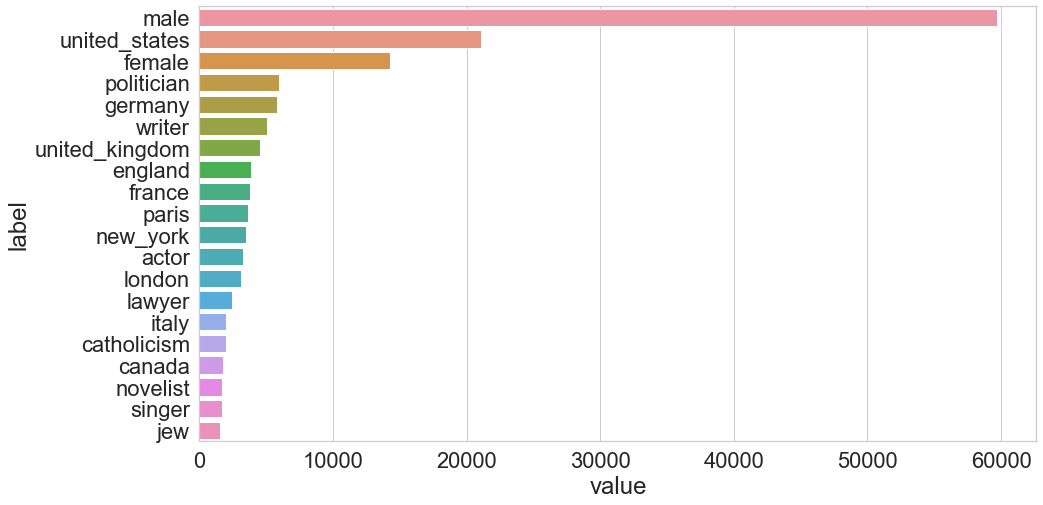
\includegraphics[width=1.0\linewidth, height=0.6\linewidth]{Freebase_Object_Counts}
		\captionsetup{justification=centering}
		\caption{Freebase}
	\end{subfigure}
	\captionsetup{justification=centering}
	\caption{Histogram showing the number of times the 20 most frequent object labels occur in KG facts, in the WordNet and Freebase link prediction datasets.}
\end{figure}

\begin{table}[H]
	\begin{center}
	\begin{tabular}{|l|ccc|ccc|}
		\hline
 		& \multicolumn{3}{c|}{\textbf{WordNet}} & \multicolumn{3}{c|}{\textbf{Freebase}} \\
		& subject & predicate & object & subject & predicate & object \\
		\hline 
		Count & 32,270 & 11 & 33,011 & 67,393 & 13 & 15,342 \\
		Max & 619 & 43,312 & 537 & 37 & 73,897 & 59,663 \\
		Min & 1 & 1,229 & 1 & 1 & 4,464 & 1 \\
		Median & 2 & 7,705 & 3 & 5 & 21,149 & 3 \\
		IQR & 2 & 7,258 & 2 & 4 & 34,033 & 6 \\
		\hline 
	\end{tabular}
	\end{center}
	\captionsetup{justification=centering}
	\caption{Statistics of the WordNet and Freebase link prediction datasets. We show counts of unique subject, predicate and object labels, as well as the maximum, minimum, median and interquartile range of label occurrences.}
\end{table}

\noindent For WordNet, it can be seen that predicates are skewed toward "has instance" with $ 43, 312 $ occurrences, and "type of" with $ 36, 659 $ occurrences. Freebase predicates are somewhat more uniform, however four predicates have occurrences under $ 10, 000 $. \par

\noindent WordNet and Freebase subjects are somewhat uniform, although the median number of occurrences is 2 and 5 respectively, with an interquartile range (IQR) of $ 2 $ and $ 4 $ respectively. WordNet object occurrences are somewhat uniform while Freebase object occurrences are skewed, with a single object, "male" occurring $ 59, 663 $ times, representing $15, 88\% $ of facts. This is in comparison to a median object occurrence of $ 3 $ and an IQR of $ 6 $. \par

\noindent The WordNet dataset is split into training, validation and test sets of $ 110, 362 \; (80.8 \%) $, $ 5, 215 \; (3.8 \%) $ and $ 21, 034 \; (15.4 \%) $ triples respectively.\ The Freebase dataset is split into training, validation and test sets of $ 316, 232 \; (84.2 \%) $, $ 11, 815 \; (3.1 \%) $ and $ 47, 452 \; (12.6 \%) $ triples respectively. 

\subsection{Baseline training algorithm}

\textbf{Model summary.} Our baseline model for this section is inspired by recursive networks (RCNs). The NTN is a bilinear tensor product between the subject, predicate and object, added to an RCN composition of the subject and object. It computes relational scores between pairs of entities. \par

\noindent \textbf{Contrastive max-margin loss.} The contrastive max-margin loss is used to train the NTN model. A relational score is computed for the target triple containing a subject, predicate and object. A relational score is then computed for the same subject and predicate, along with a non-related entity randomly selected and presented as a corrupt object. Relational scores in the range $ (-1, \; 1) $ are produced for the target and corrupt objects, respectively. The training task is to compute a large value for the target score, and small value for the corrupt score. The computed loss is backpropagated through the network to update model parameters. 


%********************************** %Optimised training algorithm **************************************

\subsection{Optimised training algorithm}

\textbf{Implementation.}\ We use the TensorFlow framework \unskip~\citep{abadi2016tensorflow} to implement our NTN training algorithms.\ The NTN model introduced by Chen et al. \unskip ~\citep{socher2013reasoning} and reimplemented in TensorFlow by Doss et al. \unskip ~\citep{Doss2015}, serves as the baseline model. We update the baseline's training algorithm by including early stopping, adaptive moment estimation (Adam) optimisation and hyperparameter random search. We also make use of the same pre-trained word vectors \unskip ~\citep{turian2010word} used to initialise entity and relational embeddings.\ The embedding parameters are adjusted during training to generate latent representations specific to a KG. The models in this section were trained on a MacBook Pro 2015 with 8 cores, 16GB RAM, and 512GB SSD, and no GPU acceleration. We evaluate the models by ranking the accuracy scores of the predicted triples for the respective test sets of WordNet and Freebase. \par

\noindent \textbf{Code to reproduce.} In the interest of reproducibility, all code needed to train and test the models in this section can be found at the following links. \newline
Baseline NTN: \url{https://github.com/xhosaBoy/recursive-neural-tensor-networks} \newline
Optimised NTN: \url{https://github.com/xhosaBoy/optimised-neural-tensor-network} 

\subsubsection{Results} 
The accuracy results of the NTN model trained using the original baseline training algorithm, compared to the optimised training algorithm are presented in Figure 4.8, as well as Table 4.2. The hypothesis outperforms the baseline accuracy across both KGs, and significantly outperforms the baseline on the WordNet KG. Hyperparameter random search seems to be responsible for this improvement, as the hypothesis begins outperforming the baseline from the first epoch. \ All experiments were only able to complete a maximum of $ 12 $ epochs before overwhelming compute resources. 

\bigskip
\bigskip

\begin{figure}[H]
	\begin{subfigure}[b]{.5\linewidth}
   		\centering
    		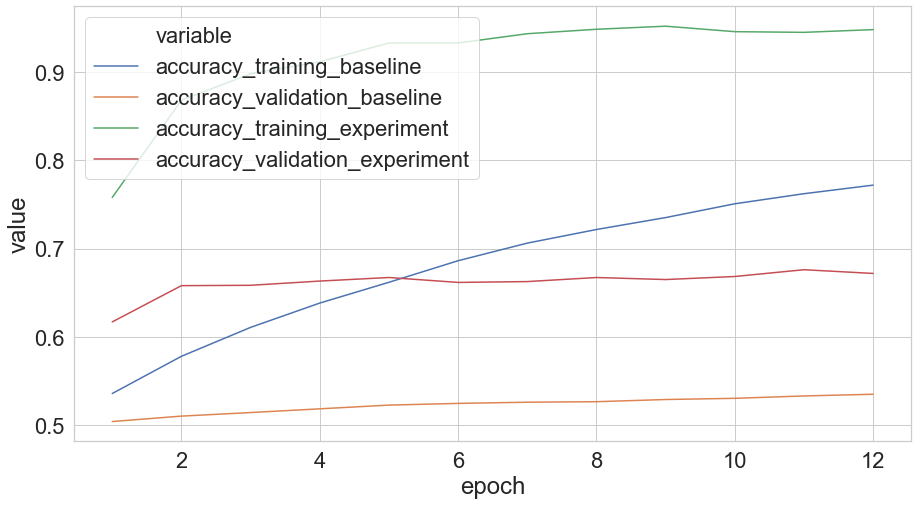
\includegraphics[width=1.0\linewidth, height=0.6\linewidth]{Wordnet_Accuracy_Results_Early_Stopping}
		\captionsetup{justification=centering}
		\caption{WordNet}
	\end{subfigure}
	\begin{subfigure}[b]{.5\linewidth}
   		\centering
		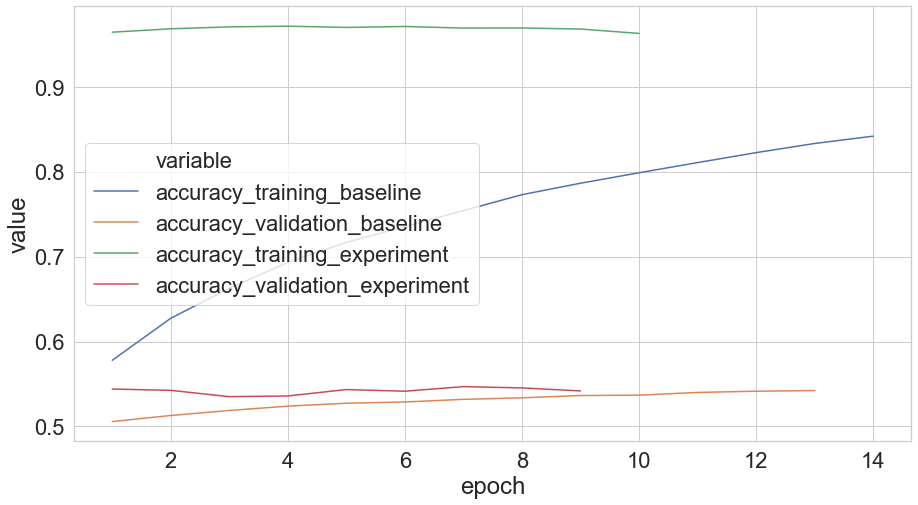
\includegraphics[width=1.0\linewidth, height=0.6\linewidth]{Freebase_Accuracy_Results}
		\captionsetup{justification=centering}
		\caption{Freebase}
	\end{subfigure}
	\captionsetup{justification=centering}
	\caption{Training and validation accuracy vs training epochs for the two datasets. The optimised algorithm performs significantly better, especially on WordNet.}
\end{figure}

\begin{table}[H]
	\centering
	\begin{tabular}{lllllllllll}
  		\textbf{Model} & \textbf{WordNet} & \textbf{Freebase} & \textbf{Avg} \\
  		\hline
  		Original NTN \unskip ~\citep{socher2013reasoning} & \textbf{.862} & \textbf{.900} & \textbf{.881} \\
  		Reimplemented NTN baseline  \unskip ~\citep{Doss2015} & .562 & .535 & .549 \\
  		\hline
  		Optimised NTN (ours) & .674 & .548 & .611 \\
		&
	\end{tabular}
	\captionsetup{justification=centering}
	\caption{Link prediction accuracy on WordNet and Freebase KG test sets. Our reimplemented NTN with the optimised training algorithm outperforms the baseline NTN, but the original NTN algorithm significantly outperforms all models. This may be due to differences in the choice of hyperparameters and optimiser, L-BFGS for the Original NTN, and Adam for the Optimised NTN. The difference between the number of iterations may also be having an impact, 500 and < 500 respectively. A slow but steady increase in the baseline and hypothesis validation accuracy can be seen before compute resources are exhausted.}
\end{table}


%********************************** %HypER and Covariate Shift  **************************************

\section{HypER and HypER+}

\subsection{Datasets} 
For the second set of experiments we use the WN18 \citep{bordes2013translating} and FB15k \citep{bordes2013translating} link prediction benchmark datasets.\ WN18 is a subset of WordNet, containing $ 40, 943 $ entities, $ 18 $ relations and 151,442 triples. FB15k is a subset of Freebase, containing $ 14, 951 $ entities, $ 1, 345 $ relations and 592,213 triples. Visualisations of the respective KGs, as well as a sample of RDF triple encoded facts, are presented in Figures 4.9 to 4.12.\ KG summary statistics are presented in Figures 4.13 to 4.16, and Table 4.3. 

\begin{figure}
   	\centering
    	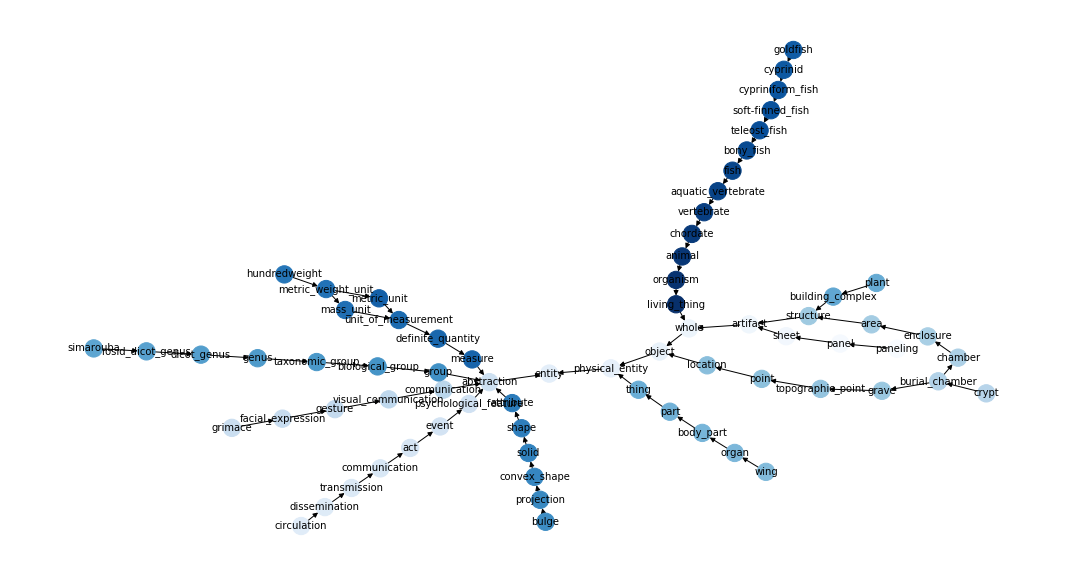
\includegraphics[width=0.9\textwidth, height=0.6\textwidth]{WN18_Graph}
	\captionsetup{justification=centering}
	\caption{A subset of WN18 facts structured as a KG. Entities are nodes, and relations are edges, where facts are encoded as RDF triples.}
\end{figure}

\begin{figure}
   	\centering
    	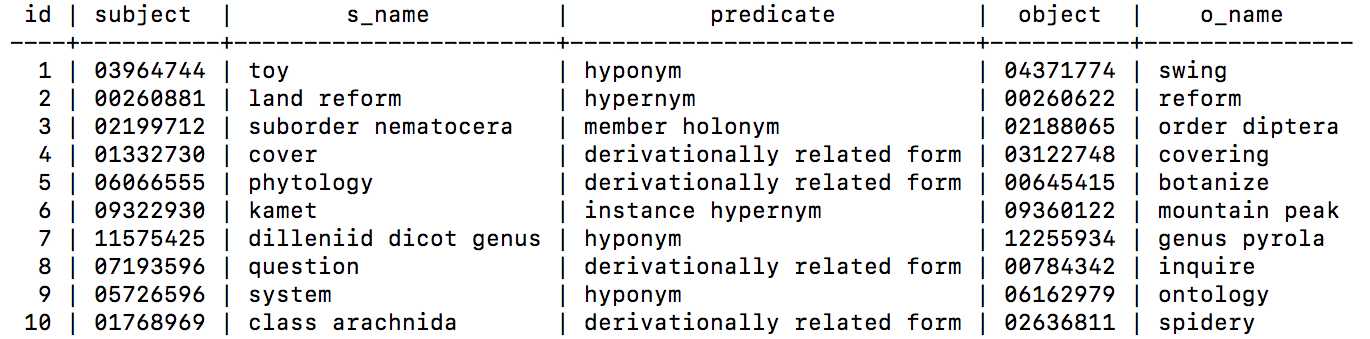
\includegraphics[width=0.9\textwidth, height=0.3\textwidth]{wn18_fact_sample}
	\captionsetup{justification=centering}
	\caption{A sample of RDF triples from the WN18 KG.}
\end{figure}

\begin{figure}[H]
   	\centering
    	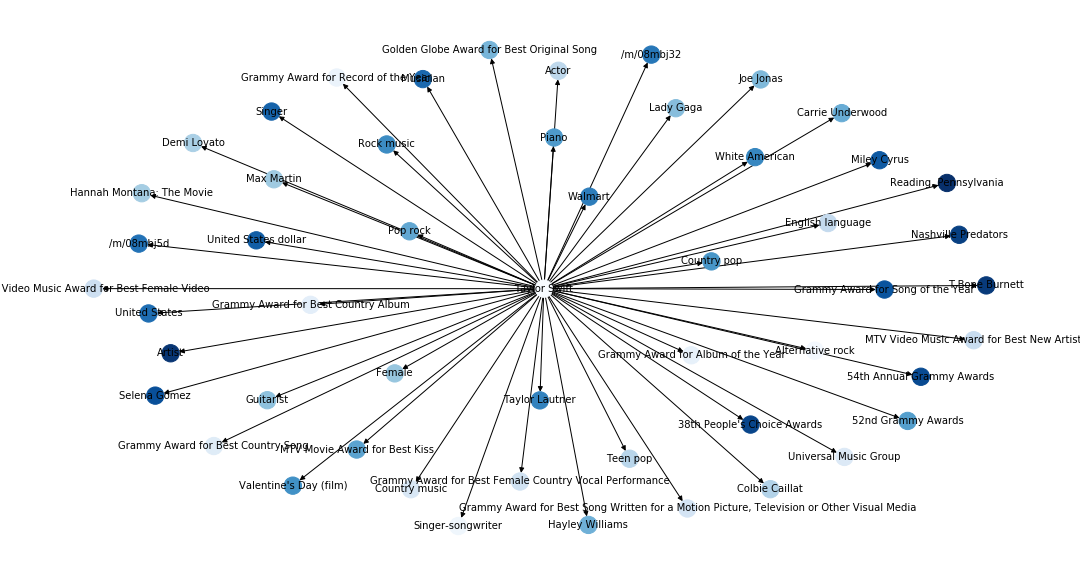
\includegraphics[width=0.9\textwidth, height=0.6\textwidth]{FB15k_Graph}
	\captionsetup{justification=centering}
	\caption{A subset of FB15k facts structured as a KG. Entities are nodes, and relations are edges, where facts are encoded as RDF triples.}
\end{figure}

\bigskip
\bigskip
\bigskip
\bigskip

\begin{figure}[H]
   	\centering
    	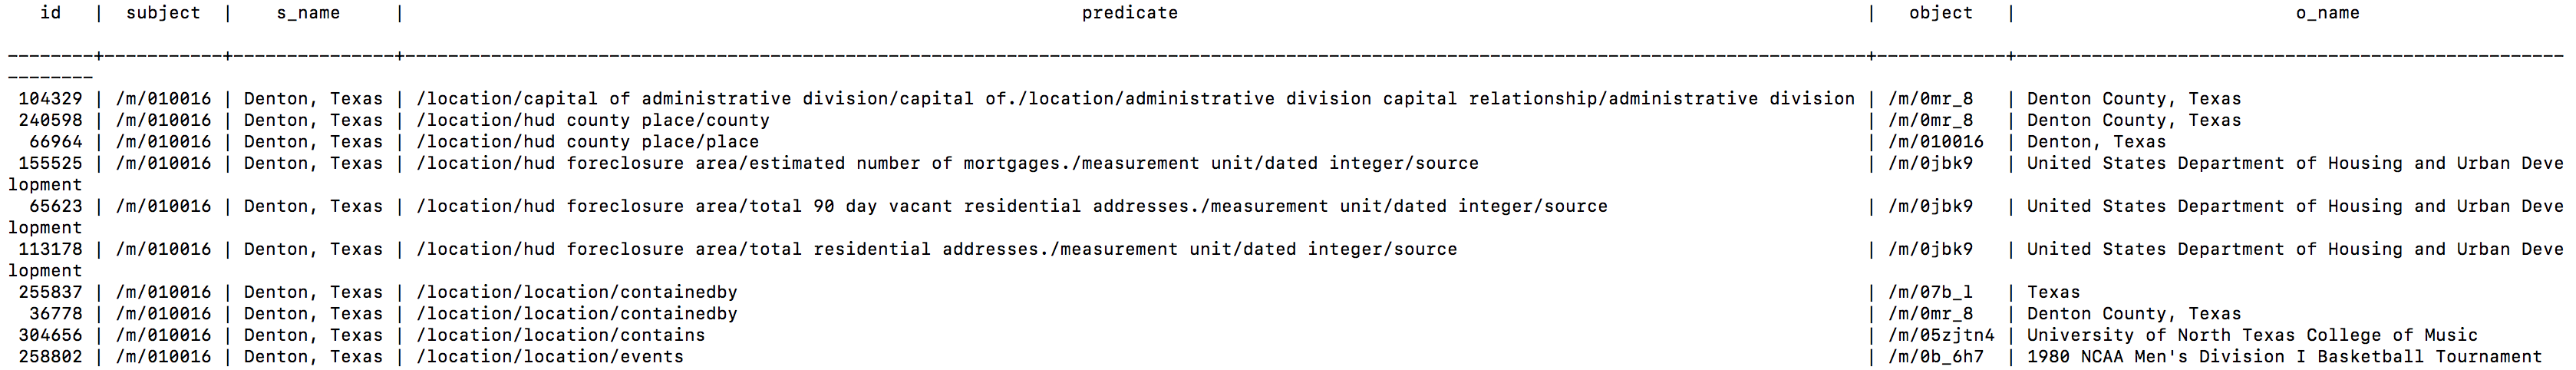
\includegraphics[width=1.0\textwidth, height=0.4\textwidth]{fb15k_fact_sample}
	\captionsetup{justification=centering}
	\caption{A sample of RDF triples from the FB15k KG.}
\end{figure}

\noindent WN18 is an intuitively usable dictionary and thesaurus, and supports automatic text analysis, while FB15k is a KG of general facts. FB15k contains more entities, relations between entities, and facts, than WN18.


%********************************** %Subject **************************************

\begin{figure}
	\begin{subfigure}[b]{.5\linewidth}
   		\centering
    		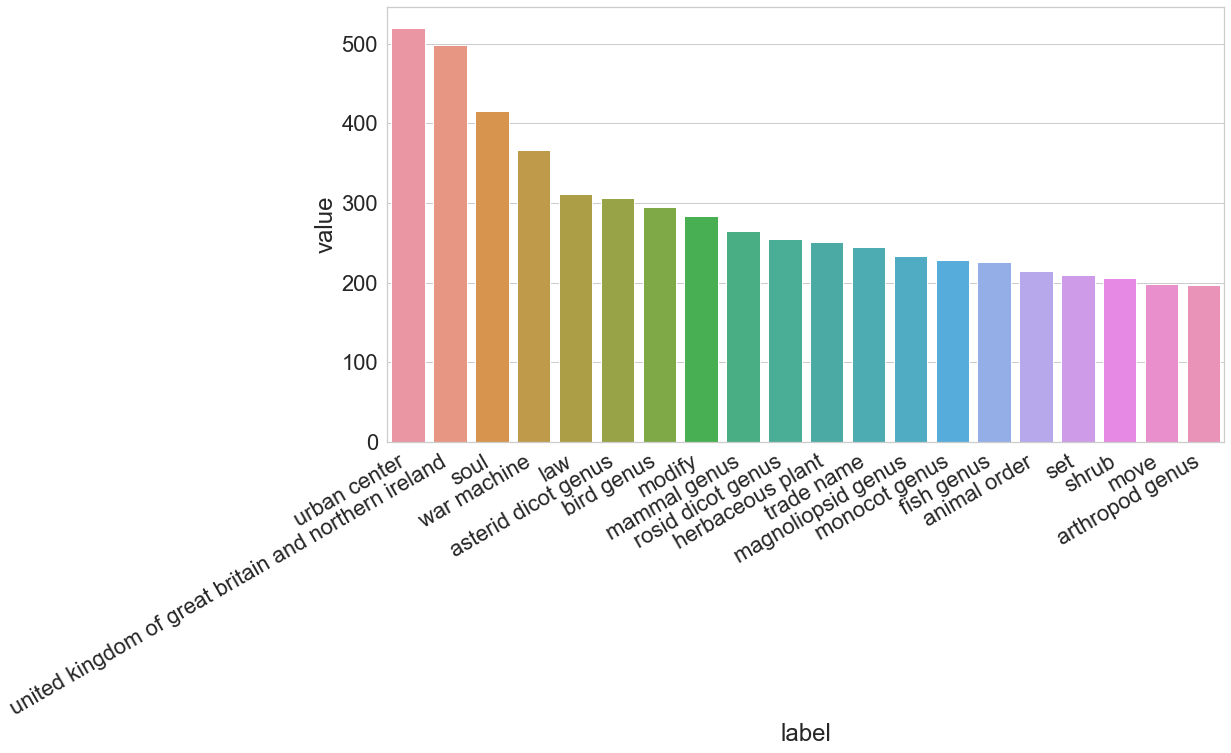
\includegraphics[width=1.0\linewidth, height=0.7\linewidth]{WN18_Subject_Counts}
		\captionsetup{justification=centering}
		\caption{WN18}
	\end{subfigure}
	\begin{subfigure}[b]{.5\linewidth}
   		\centering
		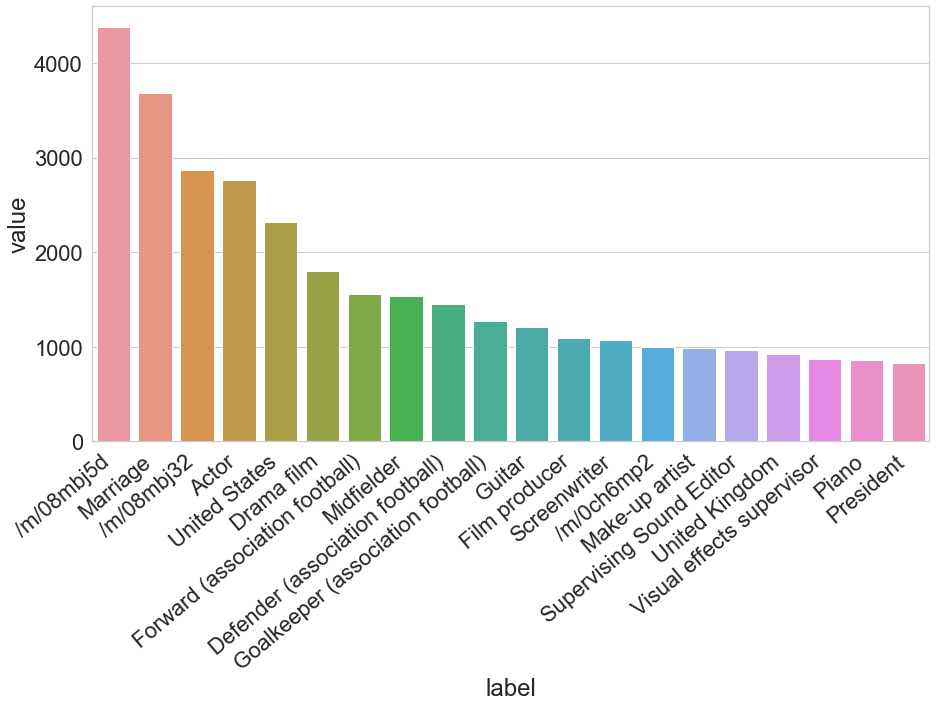
\includegraphics[width=1.0\linewidth, height=0.7\linewidth]{FB15k_Subject_Counts}
		\captionsetup{justification=centering}
		\caption{FB15k}
	\end{subfigure}
	\captionsetup{justification=centering}
	\caption{Histogram showing the number of times the 20 most frequent subject labels occur in KG facts, in the WN18 and FB15k link prediction datasets.}
\end{figure}


%********************************** %Predicate  **************************************

\begin{figure}
   	\centering
    	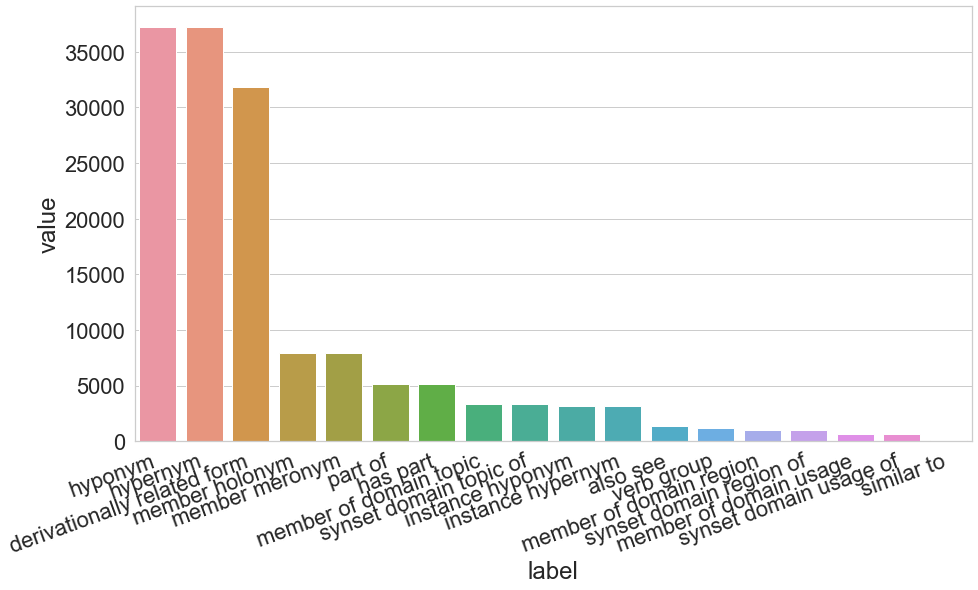
\includegraphics[width=0.7\textwidth, height=0.3\textheight]{WN18_Predicate_Counts}
	\captionsetup{justification=centering}
	\caption{Histogram showing the number of times predicate labels occur in KG facts, in the WN18 link prediction dataset.}
\end{figure}

\begin{figure}
   	\centering
    	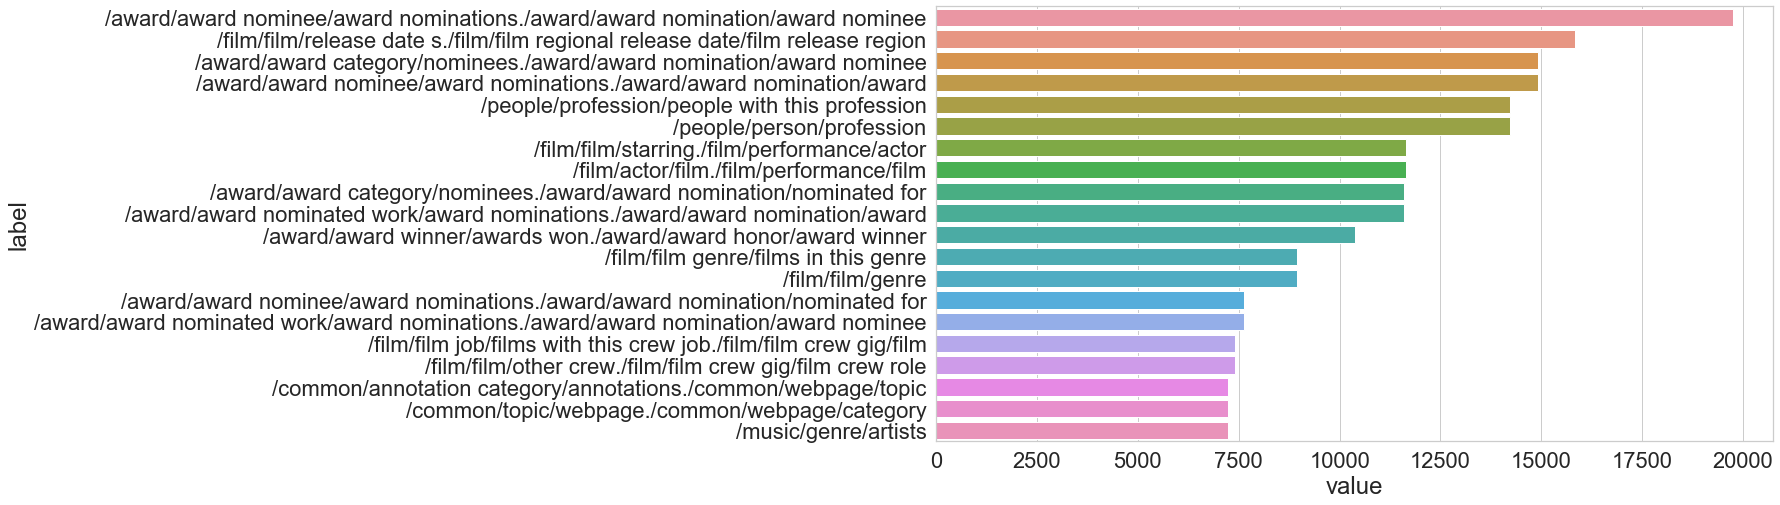
\includegraphics[width=1.0\textwidth, height=0.3\textheight]{FB15k_Predicate_Counts}
	\captionsetup{justification=centering}
	\caption{Histogram showing the number of times the 20 most frequent predicate labels occur in KG facts, in the FB15k link prediction dataset.}
\end{figure}


%********************************** %Object  **************************************

\begin{figure}
	\begin{subfigure}[b]{.5\linewidth}
   		\centering
    		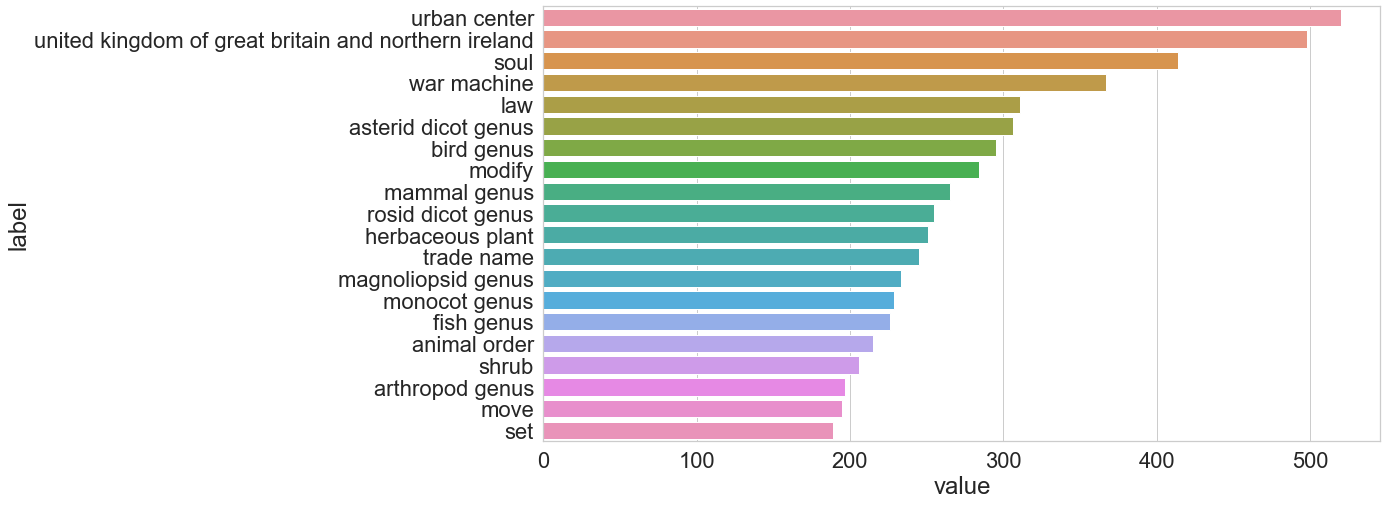
\includegraphics[width=1.0\linewidth, height=0.7\linewidth]{WN18_Object_Counts}
		\captionsetup{justification=centering}
		\caption{WN18}
	\end{subfigure}
	\begin{subfigure}[b]{.5\linewidth}
   		\centering
		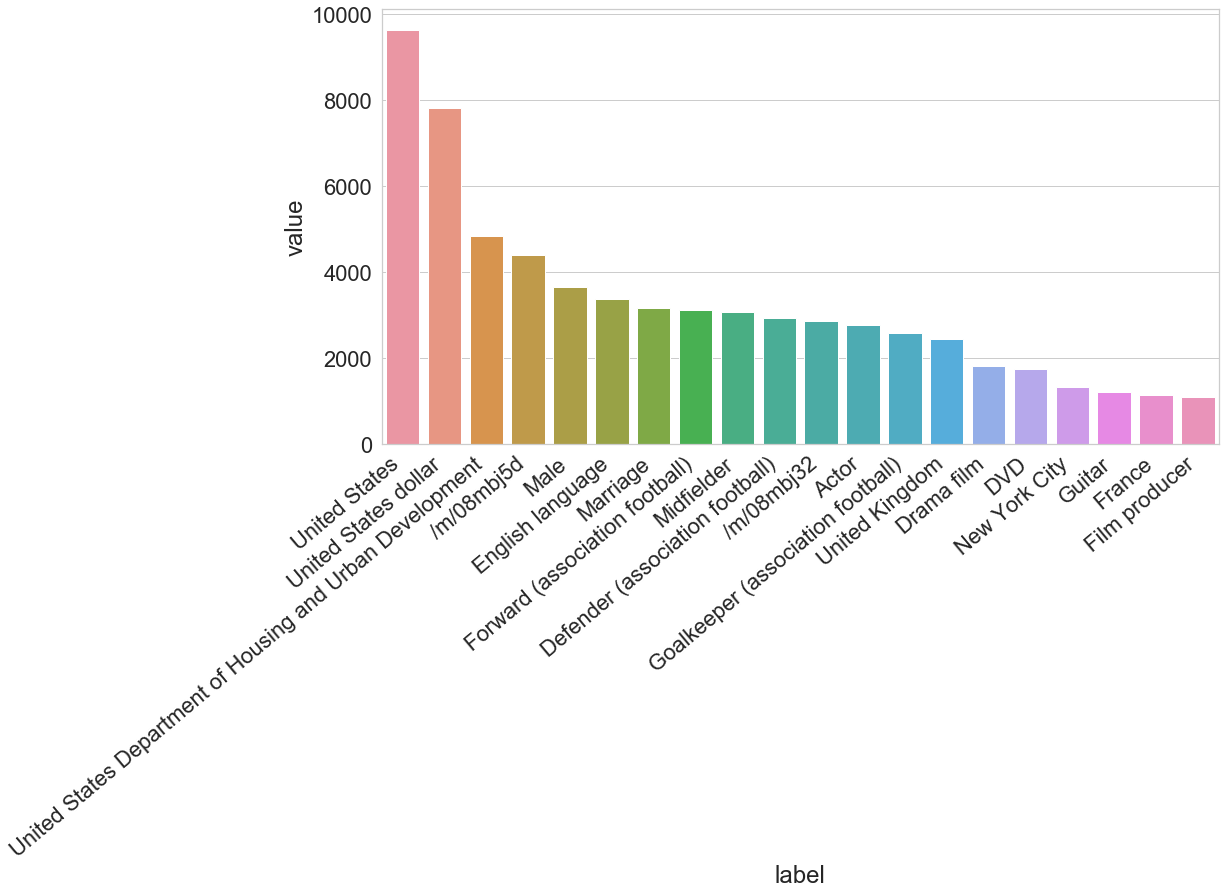
\includegraphics[width=1.0\linewidth, height=0.7\linewidth]{FB15k_Object_Counts}
		\captionsetup{justification=centering}
		\caption{FB15k}
	\end{subfigure}
	\captionsetup{justification=centering}
	\caption{Histogram showing the number of times the 20 most frequent object labels occur in KG facts, in the WN18 and FB15k link prediction datasets.}
\end{figure}

\begin{table}[H]
	\begin{center}
	\begin{tabular}{|l|ccc|ccc|}
		\hline
 		& \multicolumn{3}{c|}{\textbf{WN18}} & \multicolumn{3}{c|}{\textbf{FB15k}} \\
		& subject & predicate & object & subject & predicate & object \\
		\hline 
		Count & 32,544 & 18 & 32,543 & 14,865 & 1,345 & 14,930 \\
		Max & 520 & 37,221 & 520 & 4,381 & 19,764 & 9,645 \\
		Min & 1 & 86 & 1 & 1 & 1 & 1 \\
		Median & 3 & 3,243 & 3 & 27 & 26 & 23 \\
		IQR & 2 & 6,191 & 2 & 32 & 166 & 30 \\
		\hline 
	\end{tabular}
	\end{center}
	\captionsetup{justification=centering}
	\caption{Statistics of the WN18 and FB15k link prediction datasets. We show counts of unique subject, predicate and object labels, as well as the maximum, minimum, median and interquartile range of label occurrences.}
\end{table}

\noindent For WN18, it can be seen that predicates are skewed toward the relations "hyponym",  "hypernym", and "derivationally related from", with a maximum of $ 37, 221 $ occurrences. FB15k predicates are somewhat more uniform. \par

\noindent WN18 and FB15k subjects are somewhat uniform aside from a small number of high occurring entities, with the median number of occurrences being $ 3 $ and $ 27 $ respectively, and with an IQR of $ 2 $ and $ 32 $ respectively.\ WN18 object occurrences are somewhat uniform.\ FB15k object occurrences are skewed, with the "United States" partaking in the highest number of triples.\ This is in comparison to a median object occurrence of $ 23 $ and an IQR of 30. \par

\noindent The WN18 dataset is split into training, validation and test sets of $ 141, 442 \; (93.4 \%) $, $ 5, 000 \; (3.3 \%) $ and $ 5, 000 \; (3.3 \%) $ triples respectively.\ The FB15k dataset is split into training, validation and test sets of $ 483, 142 \; (81.6 \%) $, $ 50, 000 \; (8.4 \%) $ and $ 59, 071 \; (10.0 \%) $ triples, respectively. 

\subsection{Baseline algorithm}
\textbf{Model summary.} HypER is a model that takes the convolution between a predicate-specific filter and subject vector, to generate a subject-predicate feature map. This map is flattened and passed through a nonlinearity, before an inner product is taken with an object vector. The result is a relational score which is passed through a logistic sigmoid to generate a probability of a potential relationship between pairs of entities. \par

\noindent \textbf{Binary cross-entropy loss.} The binary cross-entropy loss is used to train HypER. Like the NTN model, the input consists of a subject-predicate pair, and an object is presented as a target to complete the triple. A relational score is generated for each sample and passed through a logistic sigmoid. Loss is generated by comparing the produced likelihood with the expected likelihood, $ 0 $ or $ 1 $. The sum of losses in a batch of samples is aggregated and backpropagated through the network for parameter update. \par

\noindent \textbf{Benchmark metrics.} The current suite of link prediction benchmark metrics includes Hit@10, Hit@3, Hit@1, Mean Rank, and Mean Reciprocal Rank.\ For these models, all objects in the KG are assigned a probability and then ranked in descending order. The Hit@X metrics comprise the relation prediction accuracy measures of the model, where X describes the lowest rank the predicted object can occupy. For example in Hit@10, only the top 10 objects are considered as accurate. The Mean Rank is the average predicted object rank and can be measured after any training epoch. The Mean Reciprocal Rank is the inverse of the Mean Rank. \par


%********************************** %HypER+  **************************************

\subsection{HypER+}

\textbf{Implementation.} Here we use the PyTorch framework to develop our model. The HypER model introduced by Bala\u{z}ev\'{i}c et al. \unskip ~\citep{balazevic2019hypernetwork} serves as a baseline. We apply batch normalisation to the hypernetwork input layer and thus introduce HypER+. Entity and relational embeddings are randomly initialised during model training. These embeddings are dynamically adjusted during the training process to generate latent representations specific to a KG. The models in this section were trained on Google Cloud Platform, on an N1 series instance with  8 CPU cores, 30GB RAM, 512GB SSD and an Nvidia Tesla P100 GPU. We train the respective models for $ 500 $ epoch, and evaluate them using the test sets of WN18 and FB15k. \par

\noindent \textbf{Code to reproduce.} In the interest of reproducibility, all code needed to train and test the models in this section can be found at the following links. \newline
Baseline HypER: \url{https://github.com/xhosaBoy/HypER-baseline} \newline
HypER+: \url{https://github.com/xhosaBoy/HypER-normalised-relations} 

\subsubsection{Results}
Results based on current standard link prediction metrics (Hit@10, Hit@3, Hit@1, Mean Rank and Mean Reciprocal Rank) for the Hyper+ model compared against the HypER model baseline, are presented in Figures 4.17 to 4.19, as well as Tables 4.4 and 4.5. T-SNE analysis \unskip ~\citep{maaten2008visualizing} of HypER+ on the FB15k KG is presented in Figures 4.20 to 4.23. \par

\noindent HypER+ achieves near-identical results with the HypER baseline on the WN18 KG across all metrics, and significantly outperforms the HypER baseline on the FB15k KG. The impact of hypernetwork batch normalisation is pronounced, perhaps due to the upstream influence of predicate input covariate shift. 

\bigskip
\bigskip


%********************************** %Hits@10  **************************************

\begin{figure}[H]
	\begin{subfigure}[b]{.5\linewidth}
   		\centering
    		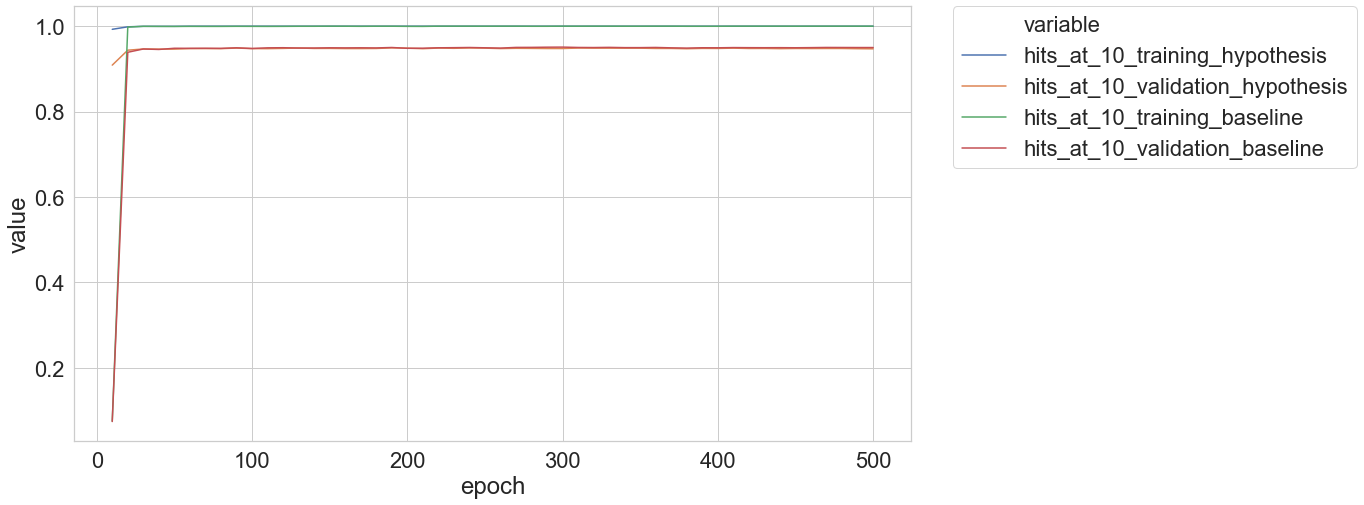
\includegraphics[width=1.0\linewidth, height=0.6\linewidth]{WN18_hits_at_10_Results}
		\captionsetup{justification=centering}
		\caption{WN18}
	\end{subfigure}
	\begin{subfigure}[b]{.5\linewidth}
   		\centering
		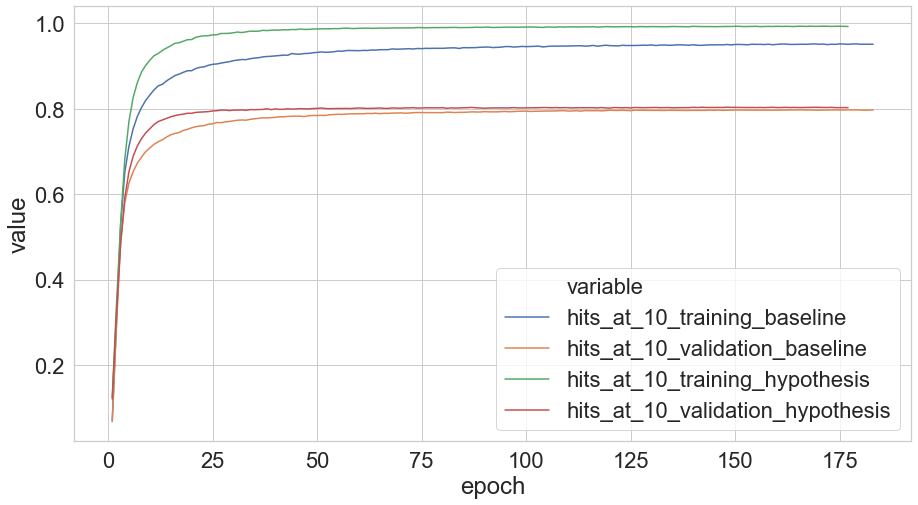
\includegraphics[width=1.0\linewidth, height=0.6\linewidth]{FB15k_hits_at_10_Results}
		\captionsetup{justification=centering}
		\caption{FB15k}
	\end{subfigure}
	\captionsetup{justification=centering}
	\caption{Hit@10 vs training epoch. There is hardly any difference between the hypothesis and baseline models for the WN18 KG. The hypothesis model outperforms the baseline on the FB15k KG, although the validation difference is not as pronounced as the training difference.}
\end{figure}

\bigskip
\bigskip
\bigskip
\bigskip


%********************************** %Hits@3  **************************************

\begin{figure}[H]
	\begin{subfigure}[b]{.5\linewidth}
   		\centering
    		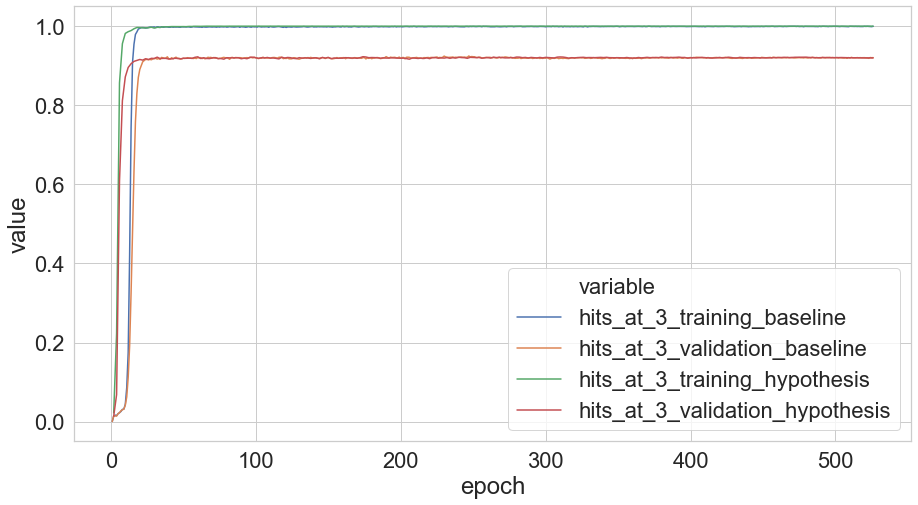
\includegraphics[width=1.0\linewidth, height=0.6\linewidth]{WN18_hits_at_3_Results}
		\captionsetup{justification=centering}
		\caption{WN18}
	\end{subfigure}
	\begin{subfigure}[b]{.5\linewidth}
   		\centering
		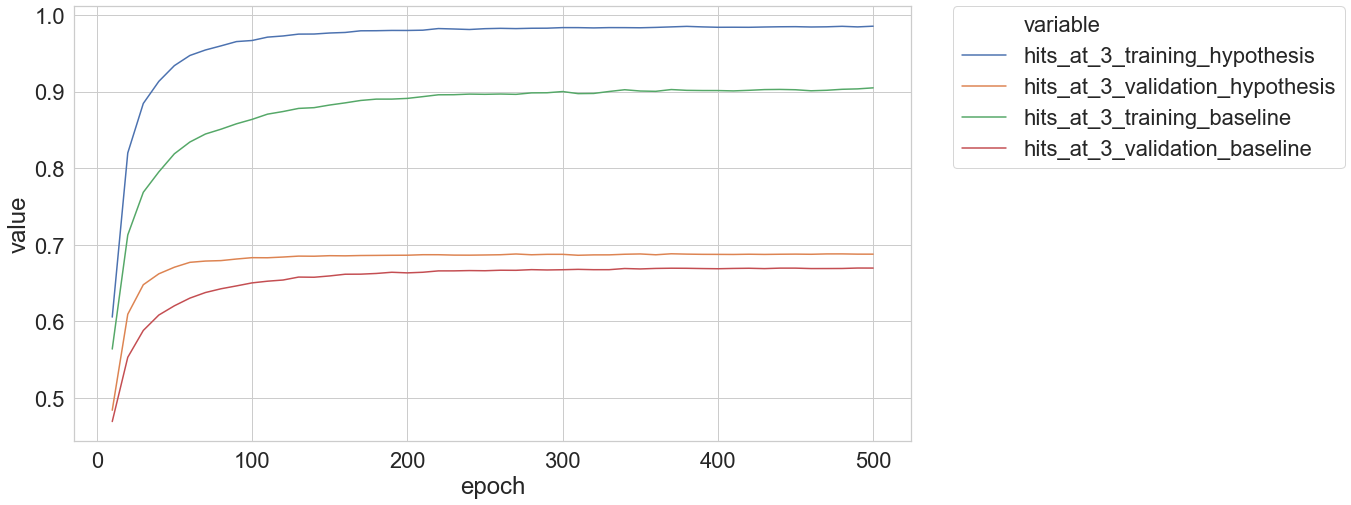
\includegraphics[width=1.0\linewidth, height=0.6\linewidth]{FB15k_hits_at_3_Results}
		\captionsetup{justification=centering}
		\caption{FB15k}
	\end{subfigure}
	\captionsetup{justification=centering}
	\caption{Hit@3 vs training epoch. The models have similar behaviour to the Hit@10 metric, and both have lower accuracy. There is however a larger performance difference between the hypothesis and baseline. This may be due to the more robust generalisation requirements with a smaller subset of acceptable answers, resulting in a more pronounced impact from covariate shift of latent predicate parameters.}
\end{figure}


%********************************** %Hits@1  **************************************

\begin{figure}[H]
	\begin{subfigure}[b]{.5\linewidth}
   		\centering
    		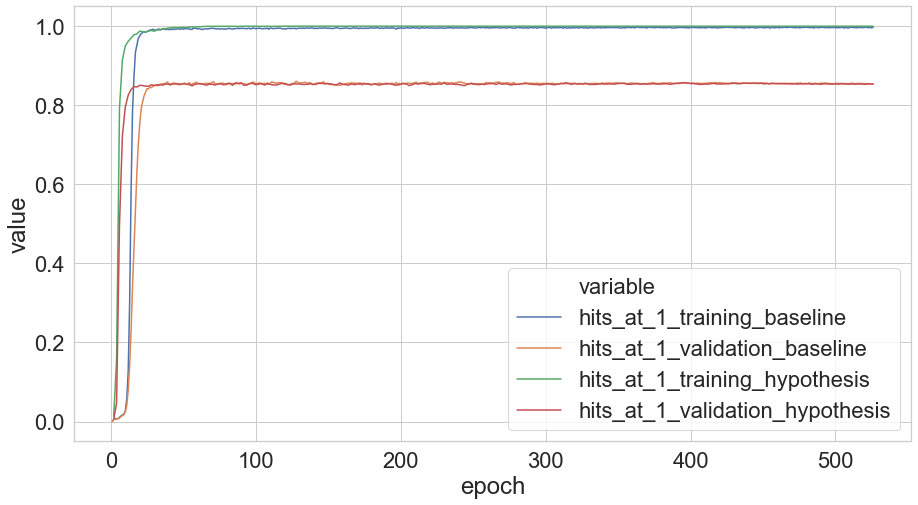
\includegraphics[width=1.0\linewidth, height=0.6\linewidth]{WN18_hits_at_1_Results}
		\captionsetup{justification=centering}
		\caption{WN18}
	\end{subfigure}
	\begin{subfigure}[b]{.5\linewidth}
   		\centering
		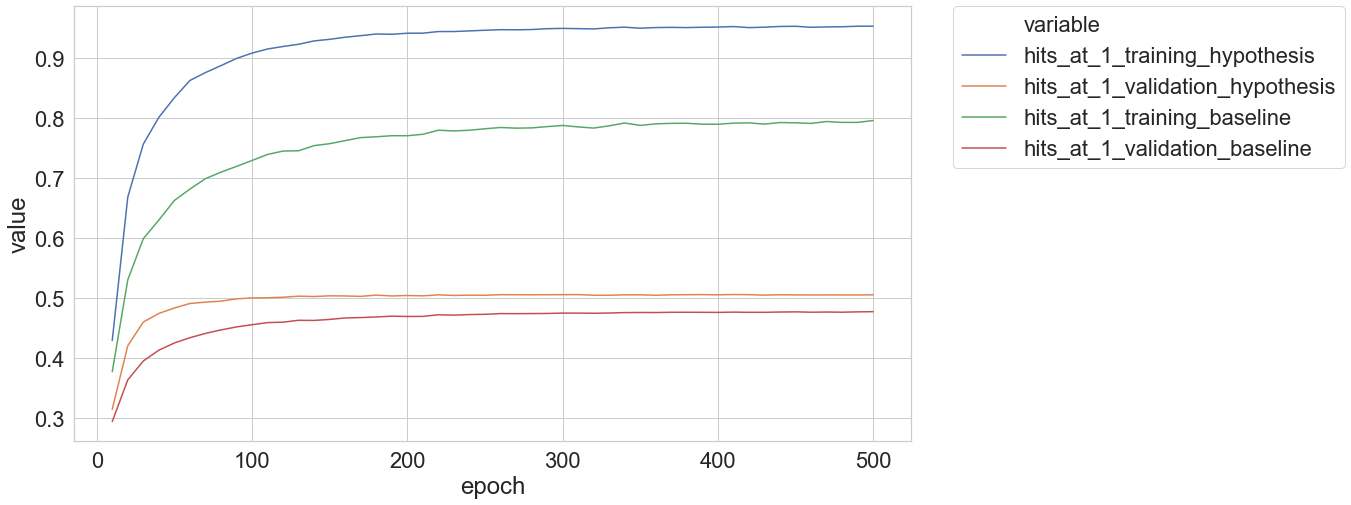
\includegraphics[width=1.0\linewidth, height=0.6\linewidth]{FB15k_hits_at_1_Results}
		\captionsetup{justification=centering}
		\caption{FB15k}
	\end{subfigure}
	\captionsetup{justification=centering}
	\caption{Hit@1 vs training epoch. The models have similar behaviour to the Hit@10 and Hit@3 metrics, and both have even lower accuracy. There is no discernible difference between the models on the WN18 KG, however there is once again a larger difference between them on the FB15k KG. }
\end{figure}

\bigskip
\bigskip
\bigskip
\bigskip


%********************************** %Test results **************************************

\begin{table}[H]
		\centering
		\begin{tabular}{lllllllllll}
  			\textbf{Model} & \textbf{H@10} & \textbf{H@3} & \textbf{H@1} & \textbf{MR} & \textbf{MRR} \\
  			\hline
  			TransE \unskip~\citep{bordes2013translating} & .892 & - & - & \textbf{251} & - \\
  			DistMult \unskip~\citep{yang2014embedding} & .936 & .914 & .728 & 902 & .822 \\
  			ComplEx \unskip~\citep{trouillon2016complex} & .947 & .936 & .936 & - & .941 \\
  			Neural LP \unskip~\citep{yang2017differentiable} & .945 & - & - & - & .940 \\
			R-GCN \unskip~\citep{schlichtkrull2018modeling} & \textbf{.964} & .929 & .697 & - & .819 \\
			TorusE \unskip~\citep{ebisu2018toruse} & .954 & .950 & .943 & - & .947 \\
			ConvE \unskip~\citep{dettmers2018convolutional} & .956 & .946 & .935 & 374 & .943 \\
			HypER \unskip~\citep{balazevic2019hypernetwork} & .958 & \textbf{.955} & \textbf{.947} & 431 & \textbf{.951} \\
  			\hline
  			HypER+ (ours) & .957 & .954 & .946 & 565 & .950 \\
			&
		\end{tabular}
		\captionsetup{justification=centering}
		\caption{Relation prediction test results on WN18. The hypothesis is outperformed by the baseline HypER model across all metrics. It should however be noted that the difference is in the order of $ 0.1\% $, indicating almost identical performance. This is consistent with training and validation results shown earlier. Interestingly, the R-GCN model achieves the highest Hit@10 performance. This model uses the graph modelling SRL paradigm, as opposed to latent feature modelling, and does perform poorly across all other metrics. There may be opportunity in exploring this paradigm further. }
\end{table}

\begin{table}
		\centering
		\begin{tabular}{lllllllllll}
  			\textbf{Model} & \textbf{H@10} & \textbf{H@3} & \textbf{H@1} & \textbf{MR} & \textbf{MRR} \\
  			\hline
  			TransE \unskip~\citep{bordes2013translating} & .471 & - & - & 125 & - \\
  			DistMult \unskip~\citep{yang2014embedding} & .824 & .733 & .546 & 97 & .654 \\
  			ComplEx \unskip~\citep{trouillon2016complex} & .840 & .759 & .599 & - & .692 \\
  			Neural LP \unskip~\citep{yang2017differentiable} & .837 & - & - & - & .760 \\
			R-GCN \unskip~\citep{schlichtkrull2018modeling} & .842 & .760 & .601 & - & .696 \\
			TorusE \unskip~\citep{ebisu2018toruse} & .832 & .771 & .674 & - & .733\\
			ConvE \unskip~\citep{dettmers2018convolutional} & .831 & .723 & .558 & 51 & .657 \\
			HypER \unskip~\citep{balazevic2019hypernetwork} & .885 & .829 & .734 & \textbf{44} & .790 \\
  			\hline
  			HypER+ (ours) & \textbf{.894} & \textbf{.856} & \textbf{.790} & 79 & \textbf{.829} \\
			&
		\end{tabular}
		\captionsetup{justification=centering}
		\caption{Relation prediction test results on FB15k. The hypothesis outperforms the baseline HypER model across all metrics, aside from Mean Rank. Unlike the performance difference on the WN18 KG, the difference here is by a number of percentage points, indicating a significant improvement over the baseline. The hypernetwork approach also significantly outperforms the R-GCN model.}
\end{table}


%********************************** %T-SNE **************************************

\begin{figure}
   	\centering
    	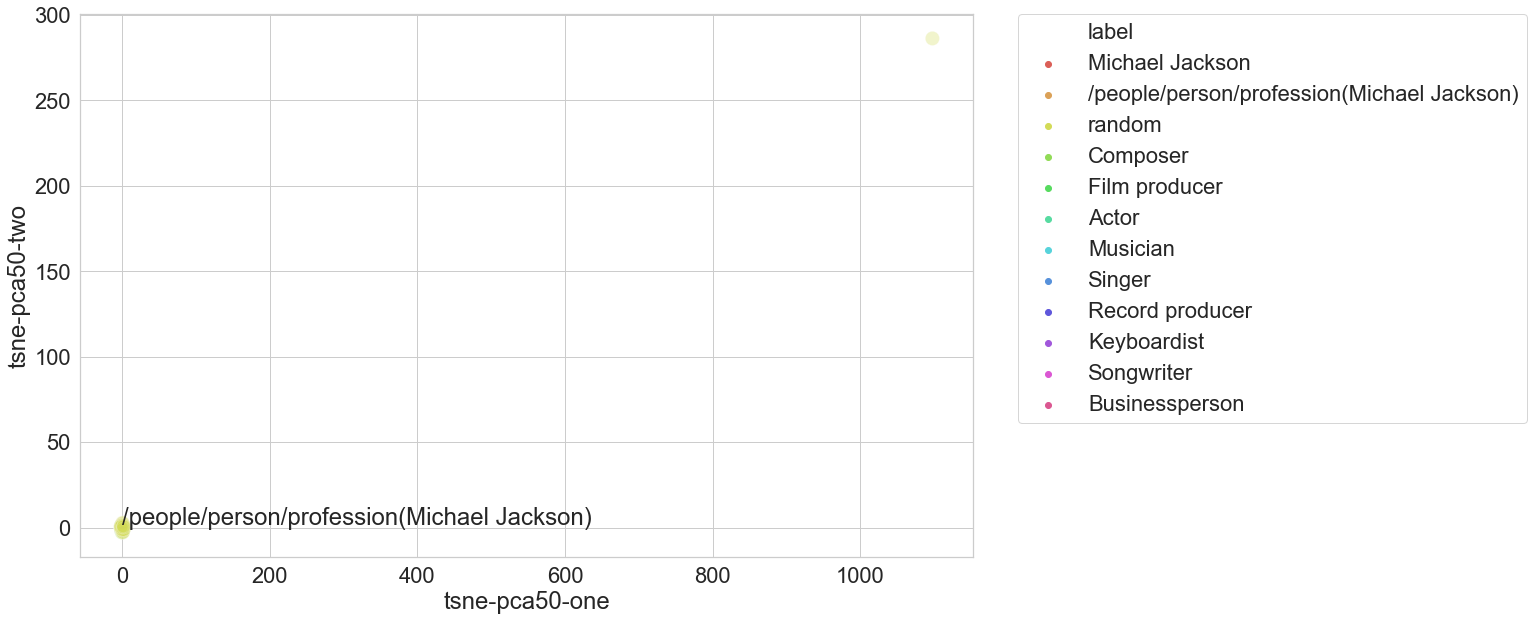
\includegraphics[width=0.7\textwidth, height=0.3\textheight]{t_sne_train_profession}
	\captionsetup{justification=centering}
	\caption{FB15k T-SNE: Triples about "Michael Jackson"'s (subject) "profession" (predicate), pre HypER+ training. The legend lists all professions (objects) known to have been performed by Michael Jackson. Most objects in the KG, regardless of type, begin clustered in the same embedding region on the bottom left. This includes the hidden subject-predicate vector,  "/people/person/profession(Michael Jackson)", used to take an inner product with an object.}
\end{figure}

\begin{figure}
   	\centering
    	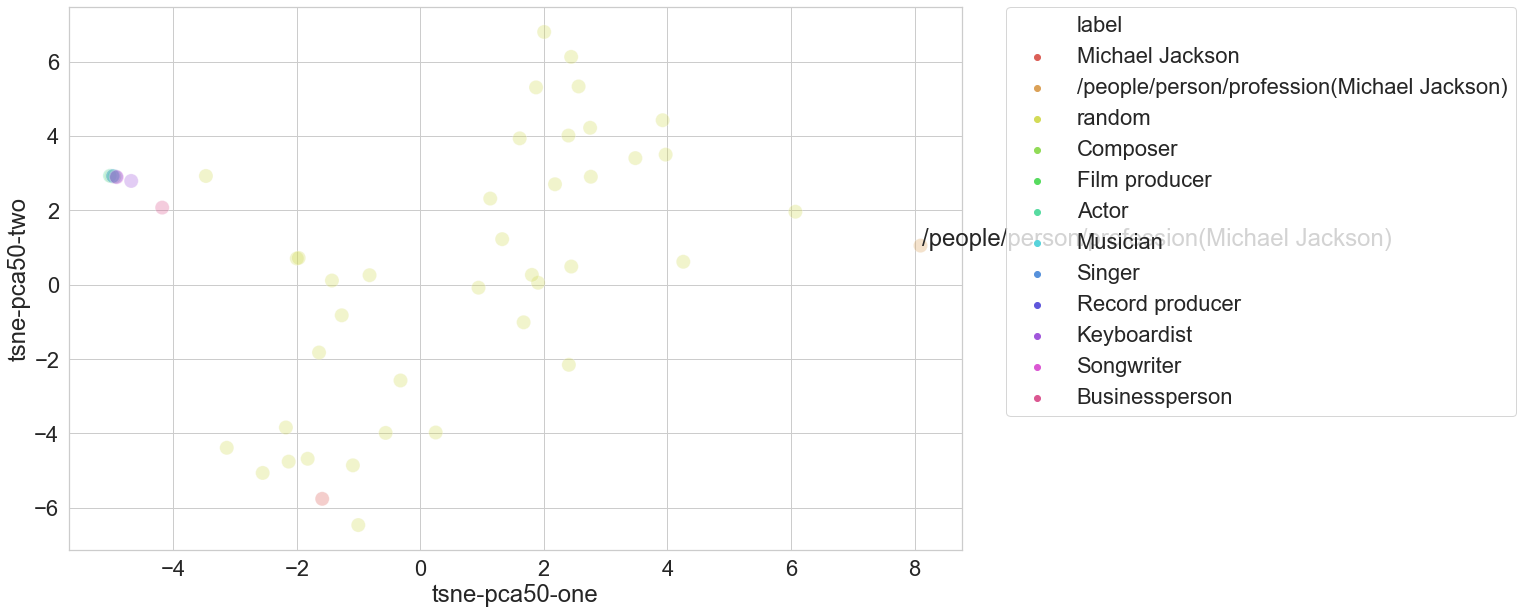
\includegraphics[width=0.7\textwidth, height=0.3\textheight]{t_sne_test_profession}
	\captionsetup{justification=centering}
	\caption{FB15k T-SNE: Triples about "Michael Jackson"'s (subject) profession (predicate), post HypER+ training. Professions Michael Jackson is known to have performed are now all clustered within the same embedding region. This indicates the model has built some conceptual understanding around the objects.}
\end{figure}

\begin{figure}
   	\centering
    	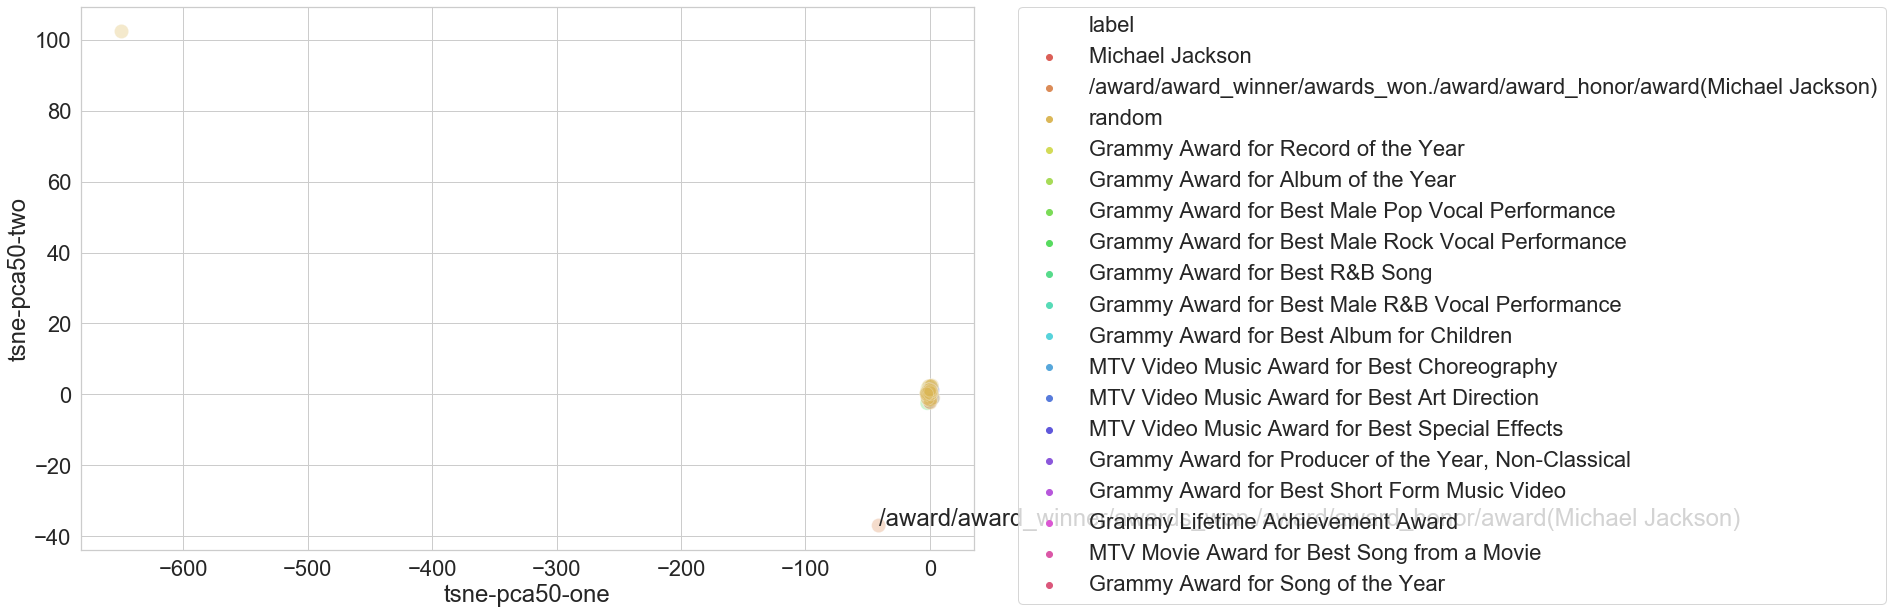
\includegraphics[width=0.7\textwidth, height=0.3\textheight]{t_sne_train_award}
	\captionsetup{justification=centering}
	\caption{FB15k T-SNE: Triples about "Michael Jackson"'s (subject) "awards" (predicate), pre HypER+ training. The legend lists all awards (objects) known to have been won by Michael Jackson. Once again most objects in the KG, regardless of type, are clustered in the same embedding region.}
\end{figure}

\begin{figure}
   	\centering
    	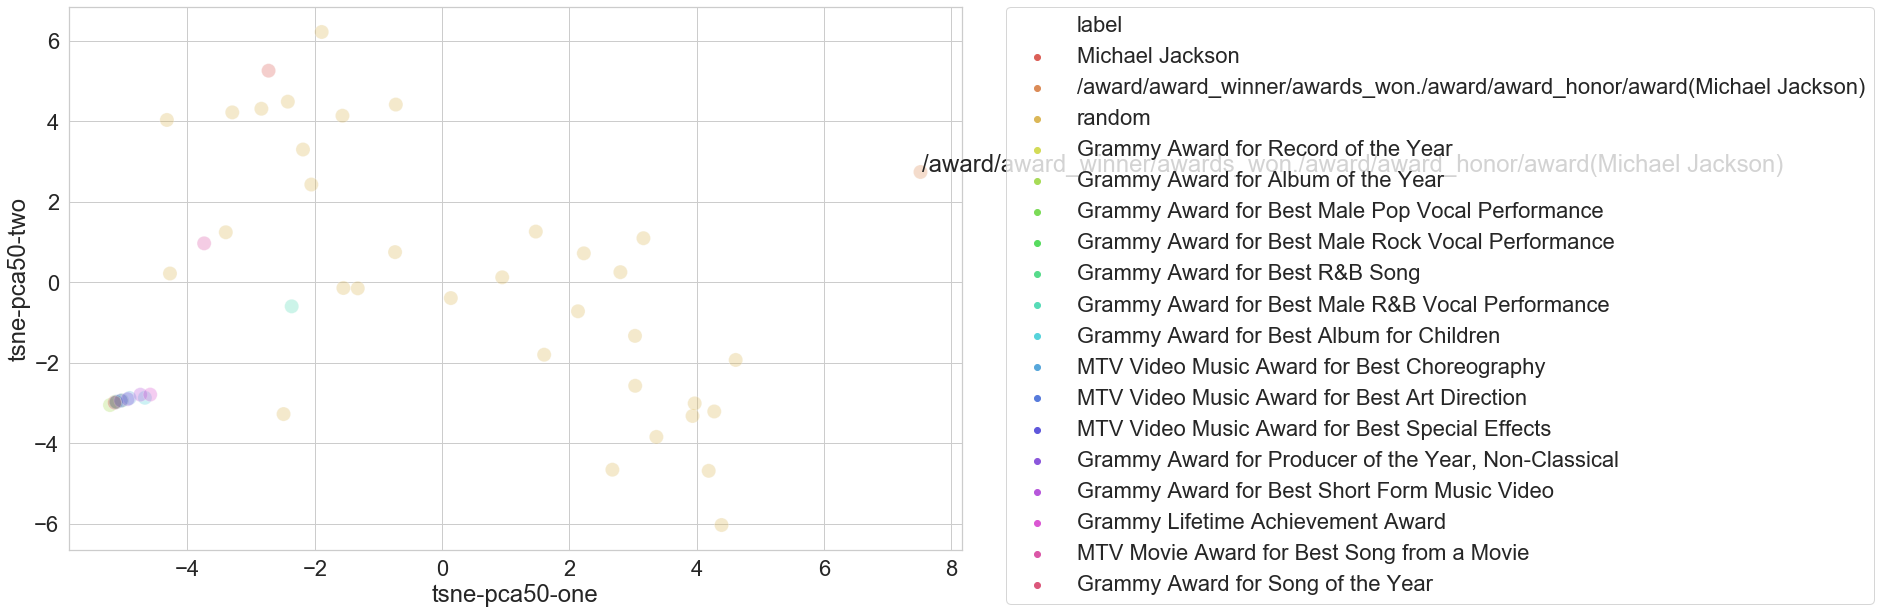
\includegraphics[width=0.7\textwidth, height=0.3\textheight]{t_sne_test_award}
	\captionsetup{justification=centering}
	\caption{FB15k T-SNE: Triples about "Michael Jackson"'s (subject) "awards" (predicate), post HypER+ training. Awards Michael Jackson is known to have won are now somewhat clustered within the same embedding region. This indicates the model has built some conceptual understanding around the objects, and attempts to account for sub-domain differences, as well as conceptual differences between the awards. For example, the "MTV Movie Award for Best Song from a Movie" is located in a region relatively far from all the "Music"-related awards.}
\end{figure}


%********************************** %HypER+ with Pre-Trained Word Embeddings  **************************************

\section{HypER+ with pre-trained word vectors}

\subsection{Datasets} 
For the third and final set of experiments we use the WN18RR and FB15k-237 benchmark datasets.\ WN18RR is a subset of WN18, created by Dettmers et al. \unskip~\citep{dettmers2018convolutional} through removing the inverse relations from WN18. WN18RR contains $ 40, 943 $ entities, $ 11 $ relations and $ 40,943 $ triples. FB15k-237 was created by Toutanova et al. \unskip~\citep{toutanova2015observed}, who noted that the validation and test sets of FB15k and WN18 contain the inverse of many relations present in the training set, making it easy for simple models to do well. FB15k-237 is a subset of FB15k with the inverse relations removed. It contains $ 14, 541 $ entities, $ 237 $ relations and $ 14,541 $ triples. Visualisations of the respective KGs, as well as a sample of RDF triple encoded facts, are presented in Figures 4.26 to 4.29. KG summary statistics are presented in Figures 4.30 to 4.33, and Table 4.6. 

\begin{figure}
   	\centering
    	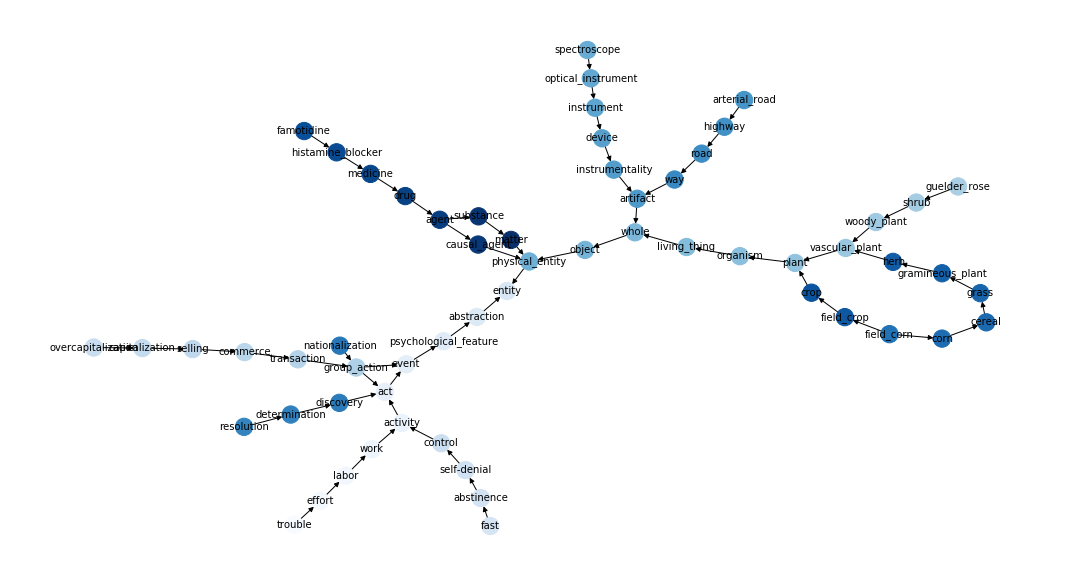
\includegraphics[width=0.9\textwidth, height=0.6\textwidth]{WN18RR_Graph}
	\captionsetup{justification=centering}
	\caption{A subset of WN18RR facts structured as a KG. Entities are nodes, and relations are edges, where facts are encoded as RDF triples.}
\end{figure}

\begin{figure}
   	\centering
    	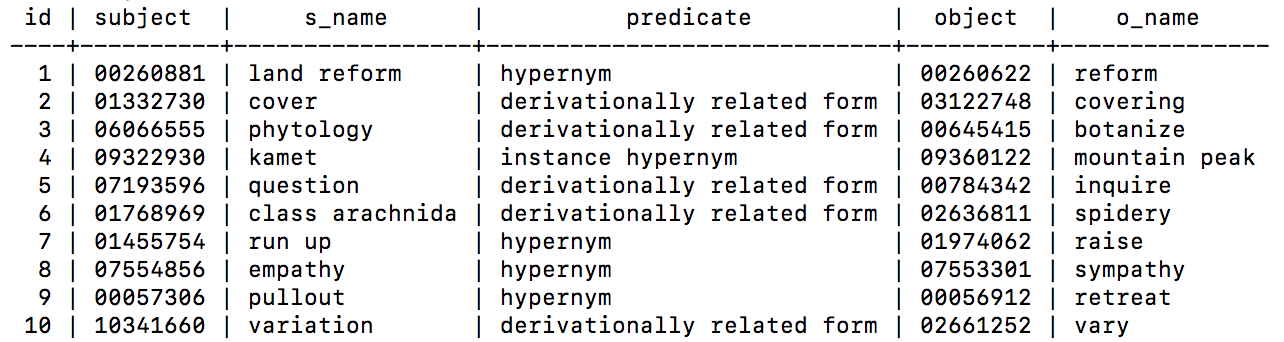
\includegraphics[width=0.9\textwidth, height=0.3\textwidth]{wn18rr_fact_sample}
	\captionsetup{justification=centering}
	\caption{A sample of RDF triples from the WN18RR KG.}
\end{figure}

\begin{figure}[H]
   	\centering
    	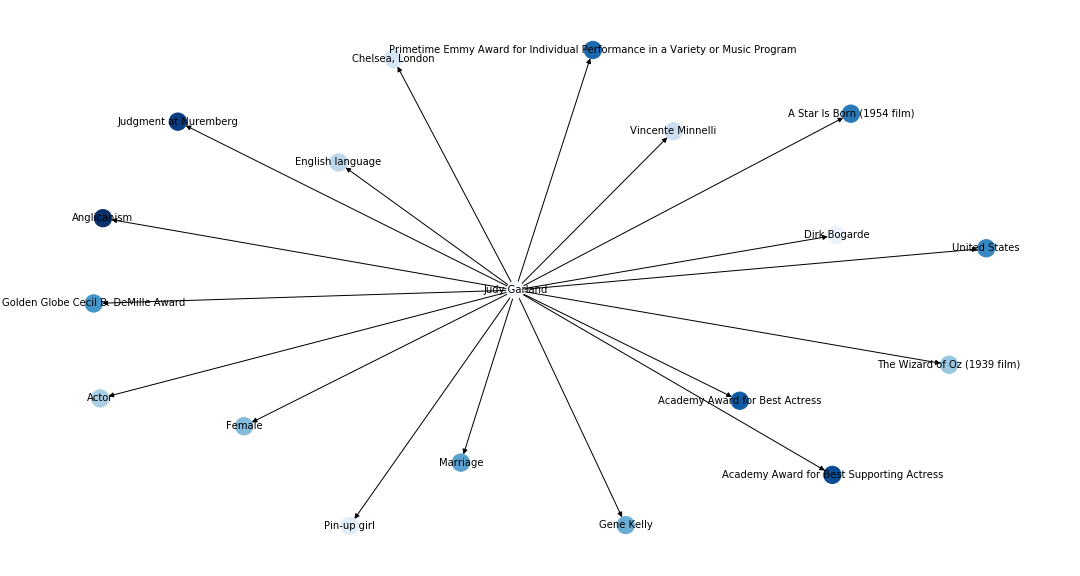
\includegraphics[width=0.9\textwidth, height=0.6\textwidth]{FB15k-237_Graph}
	\captionsetup{justification=centering}
	\caption{A subset of FB15k-237 facts structured as a KG. Entities are nodes, and relations are edges, where facts are encoded as RDF triples.}
\end{figure}

\bigskip
\bigskip
\bigskip
\bigskip

\begin{figure}[H]
   	\centering
    	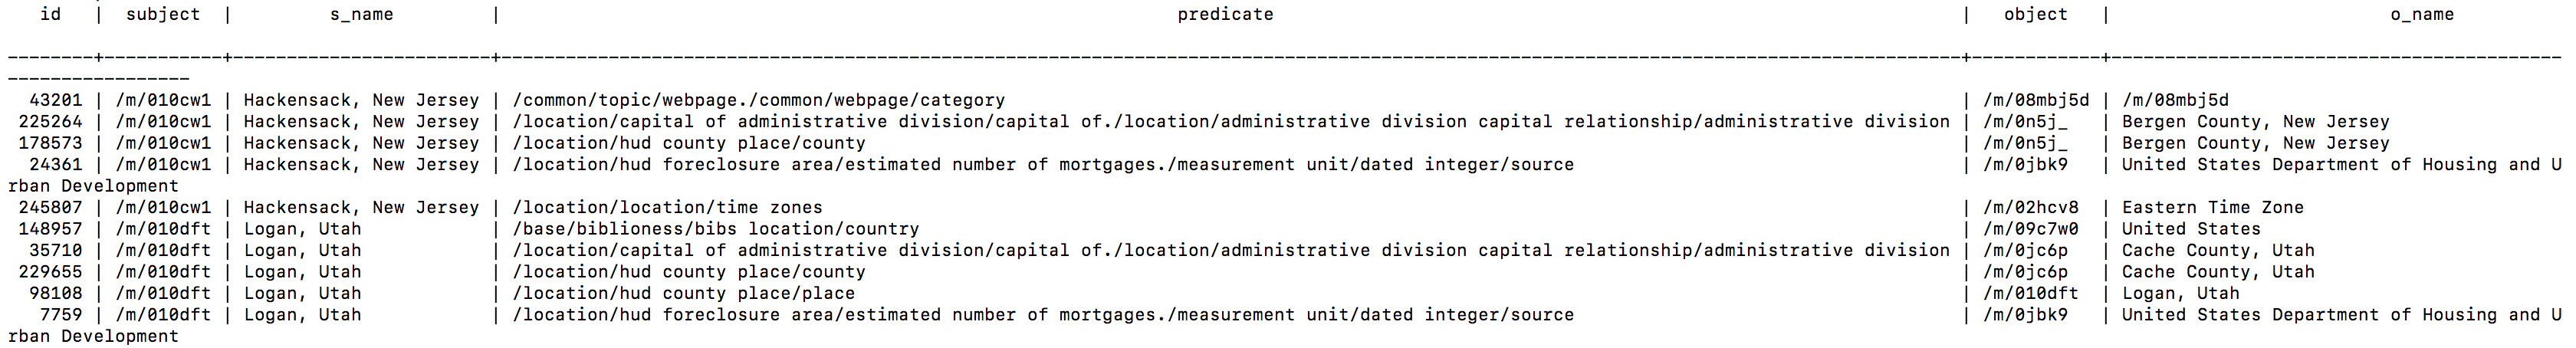
\includegraphics[width=1.0\textwidth, height=0.3\textwidth]{fb15k_237_fact_sample}
	\captionsetup{justification=centering}
	\caption{A sample of RDF triples from the FB15k-237 KG.}
\end{figure}

\noindent Once again FB15k-237 contains more entities, relations between entities, and facts, than WN18RR.

%********************************** %Subject **************************************

\begin{figure}
	\begin{subfigure}[b]{.5\linewidth}
   		\centering
    		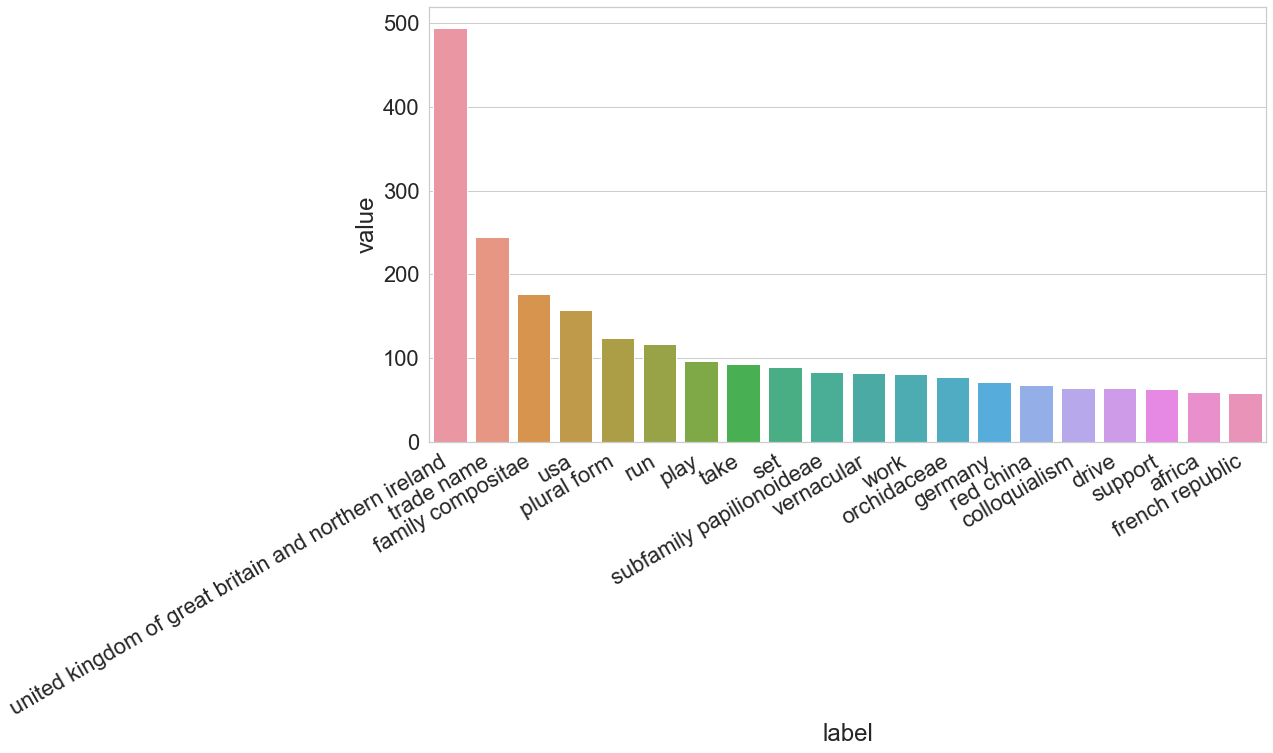
\includegraphics[width=1.0\linewidth, height=0.7\linewidth]{WN18RR_Subject_Counts}
		\captionsetup{justification=centering}
		\caption{WN18RR}
	\end{subfigure}
	\begin{subfigure}[b]{.5\linewidth}
   		\centering
		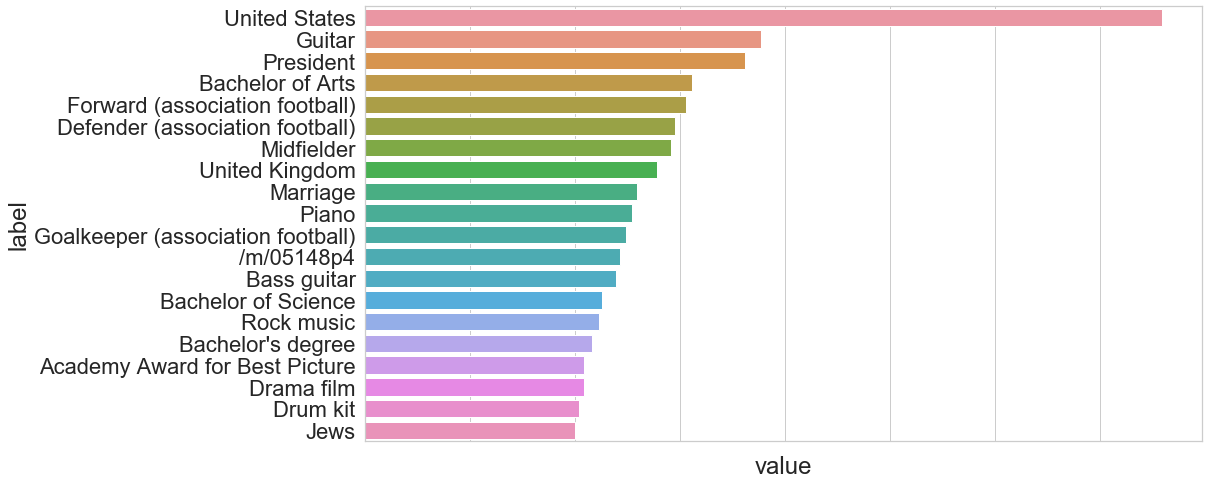
\includegraphics[width=1.0\linewidth, height=0.7\linewidth]{FB15k-237_Subject_Counts}
		\captionsetup{justification=centering}
		\caption{FB15k-237}
	\end{subfigure}
	\captionsetup{justification=centering}
	\caption{Histogram showing the number of times the 20 most frequent subject labels occur in KG facts, in the WN18RR and FB15k-237 link prediction datasets.}
\end{figure}

\bigskip
\bigskip


%********************************** %Predicate **************************************

\begin{figure}
   	\centering
    	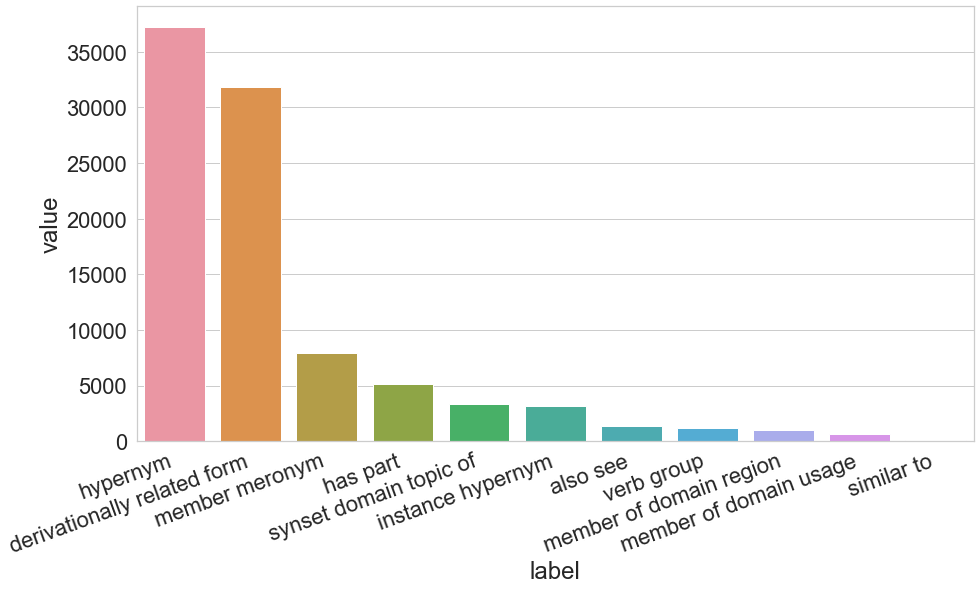
\includegraphics[width=0.7\textwidth, height=0.3\textheight]{WN18RR_Predicate_Counts}
	\captionsetup{justification=centering}
	\caption{Histogram showing the number of times predicate labels occur in KG facts, in the WN18RR link prediction dataset.}
\end{figure}

\begin{figure}
   	\centering
    	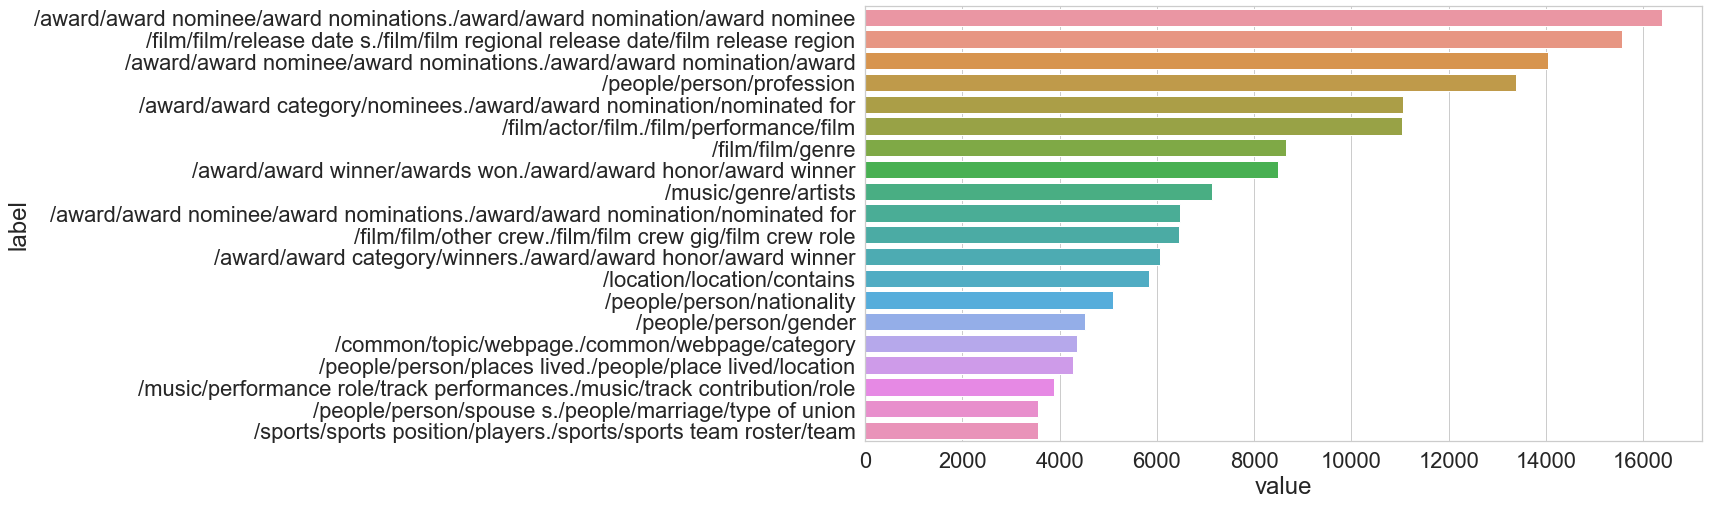
\includegraphics[width=1.0\textwidth, height=0.3\textheight]{FB15k-237_Predicate_Counts}
	\captionsetup{justification=centering}
	\caption{Histogram showing the number of times the 20 most frequent predicate labels occur in KG facts, in the FB15k-237 link prediction dataset.}
\end{figure}


%********************************** %Object **************************************

\begin{figure}
	\begin{subfigure}[b]{.5\linewidth}
   		\centering
    		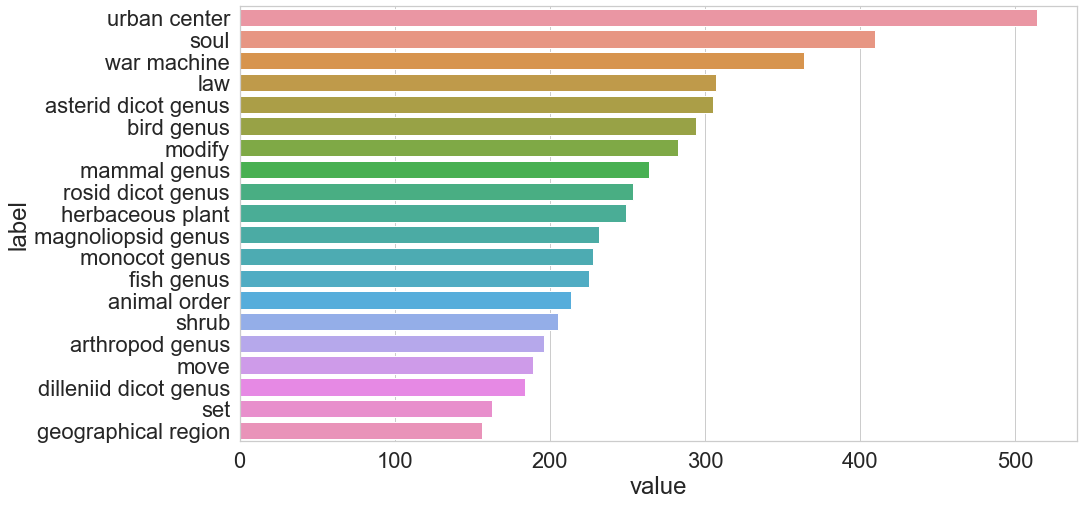
\includegraphics[width=1.0\linewidth, height=0.7\linewidth]{WN18RR_Object_Counts}
		\captionsetup{justification=centering}
		\caption{WN18RR}
	\end{subfigure}
	\begin{subfigure}[b]{.5\linewidth}
   		\centering
		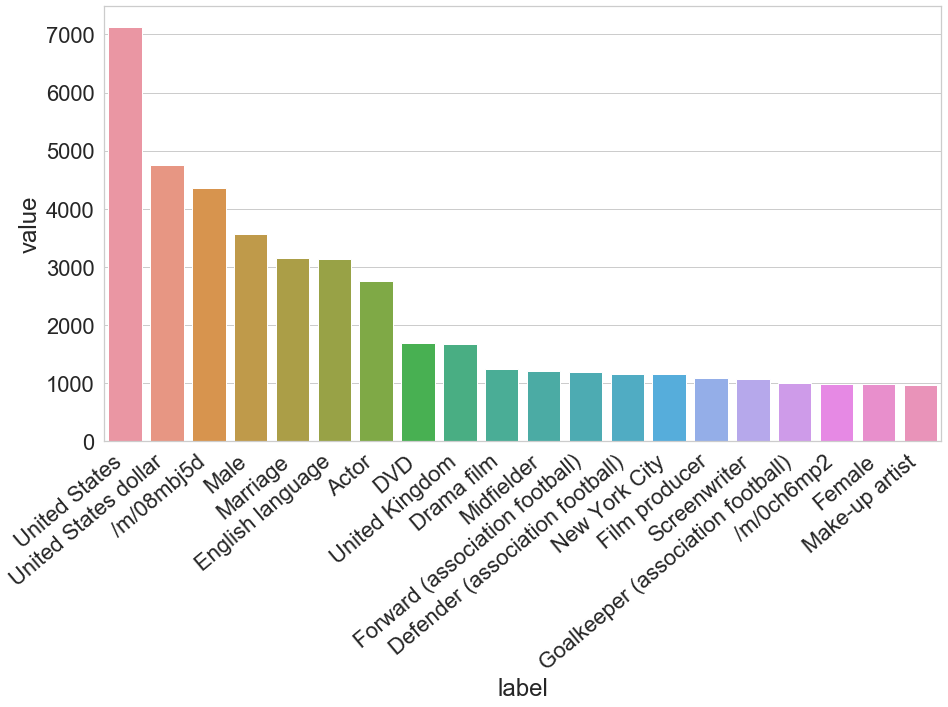
\includegraphics[width=1.0\linewidth, height=0.7\linewidth]{FB15k-237_Object_Counts}
		\captionsetup{justification=centering}
		\caption{FB15k-237}
	\end{subfigure}
	\captionsetup{justification=centering}
	\caption{Histogram showing the number of times the 20 most frequent object labels occur in KG facts, in the WN18RR and FB15k-237 link prediction datasets.}
\end{figure}

\begin{table}[H]
	\begin{center}
	\begin{tabular}{|l|ccc|ccc|}
		\hline
 		& \multicolumn{3}{c|}{\textbf{WN18RR}} & \multicolumn{3}{c|}{\textbf{FB15k-237}} \\
		& subject & predicate & object & subject & predicate & object \\
		\hline 
		Count & 32,349 & 11 & 26,162 & 13,891 & 237 & 13,504 \\
		Max & 494 & 37,221 & 514 & 1,518 & 16,391 & 7,124 \\
		Min & 1 & 86 & 1 & 1 & 45 & 1 \\
		Median & 2 & 3150 & 1 & 16 & 426 & 10 \\
		IQR & 2 & 5434 & 2 & 20 & 819 & 16 \\
		\hline 
	\end{tabular}
	\end{center}
	\captionsetup{justification=centering}
	\caption{Statistics of the WN18RR and FB15k-237 link prediction datasets. We show counts of unique subject, predicate and object labels, as well as the maximum, minimum, median and interquartile range of label occurrences.}
\end{table}

\noindent For WN18RR, it can be seen that predicates are skewed toward the relations "hypernym" and "derivationally related from", with a maximum of $ 37, 221 $ occurring, and an IQR of $ 5434 $ and $ 819 $ respectively. FB15k-237 predicates are skewed toward the film relation. \par

\noindent WN18RR and FB15k-237 subjects are somewhat uniform aside from a small number of high occurring entities, with the median number of occurrences being $ 2 $ and $ 16 $ respectively, and with an IQR of $ 2 $ and $ 20 $ respectively. WN18RR object occurrences are also somewhat uniform, while FB15k-237 object occurrences are skewed, with the "United States" partaking in the highest number of triples. This is in comparison to a median object occurrence of $ 1 $ and $ 10 $, and an IQR of $ 2 $ and $ 16 $ respectively. \par

\noindent The WN18RR dataset is split into training, validation and test sets of $ 86, 835 \; (93.4 \%) $, $ 3, 034 \; (3.3 \%) $ and $ 3, 134\; (3.4 \%) $ triples respectively.\ The FB15k-237 dataset is split into training, validation and test sets of $ 272, 115 \; (87.8 \%) $, $ 17, 535 \; (5.7 \%) $ and $ 20, 466 \; (6.6 \%) $ triples respectively.

\subsection{Baseline algorithm}
\textbf{Model summary.} HypER+, introduced in Section 4.2.3, is a model which compensates for covariate shift caused by hypernetworks, by applying batch normalisation to the hypernetwork input layer. The same algorithm as the HypER model is then used to produce a relational score, which is passed through a logistic sigmoid to generate a probability of a potential relationship between pairs of entities.\ HypER+ makes use of Xavier initialised entity and relation embeddings, and is trained using the binary cross-entropy loss. \par


%********************************** %Pre-Trained Word Embeddings **************************************

\subsection{GloVe word vector initialisation}

\textbf{Implementation.} We use the PyTorch framework to develop the HypER+ model with pre-trained embeddings, which is built on top of HypER+.\ Pre-trained GloVe word vectors replace Xavier initialised entity and relational embeddings for model training.\ These embeddings are dynamically adjusted during the training process to generate latent representations specific to the KG. The models in this section were trained on Google Cloud Platform, on an N1 series instance with  8 CPU cores, 30GB RAM, 512GB SSD and an Nvidia Tesla P100 GPU. We train the respective models for $ 500 $ epoch, and evaluate them using the test sets of WN18RR and FB15k-237. \par 

\noindent \textbf{Code to reproduce.} In the interest of reproducibility, all code needed to train and test the models in this section can be found at the following links. \newline
Baseline HypER+: \url{https://github.com/xhosaBoy/HypER-normalised-relations} \newline
HypER+ with GloVe word vectors: \url{https://github.com/xhosaBoy/HypER-pretrained-word-vectors} \par

\subsubsection{Results}
Current standard link prediction metrics (Hit@10, Hit@3, Hit@1, Mean Rank and Mean Reciprocal Rank) are used to first compare the HypER+ model without pre-trained embeddings gainst the HypER+ model with pre-trained embeddings. The results are presented in Figures 4.32 and 4.33, as well as Tables 4.7 and 4.8. Qualitative results are presented in Figure 4.34 and Table 4.9. \par

\noindent HypER+ with pre-trained embeddings gives state-of-the-art (SOTA) performance across both WN18RR and FB15k-237.\ Pre-trained word embeddings have a particularly pronounced impact on the WN18RR Hit@10 and Hit@3 metrics, perhaps due to the smaller number of samples in this KG. They however have limited impact on the Hit@1 metric, where HypER+ without pre-trained embeddings achieves SOTA performance.


%********************************** %Hits@10 **************************************

\begin{figure}
	\begin{subfigure}[b]{.5\linewidth}
   		\centering
    		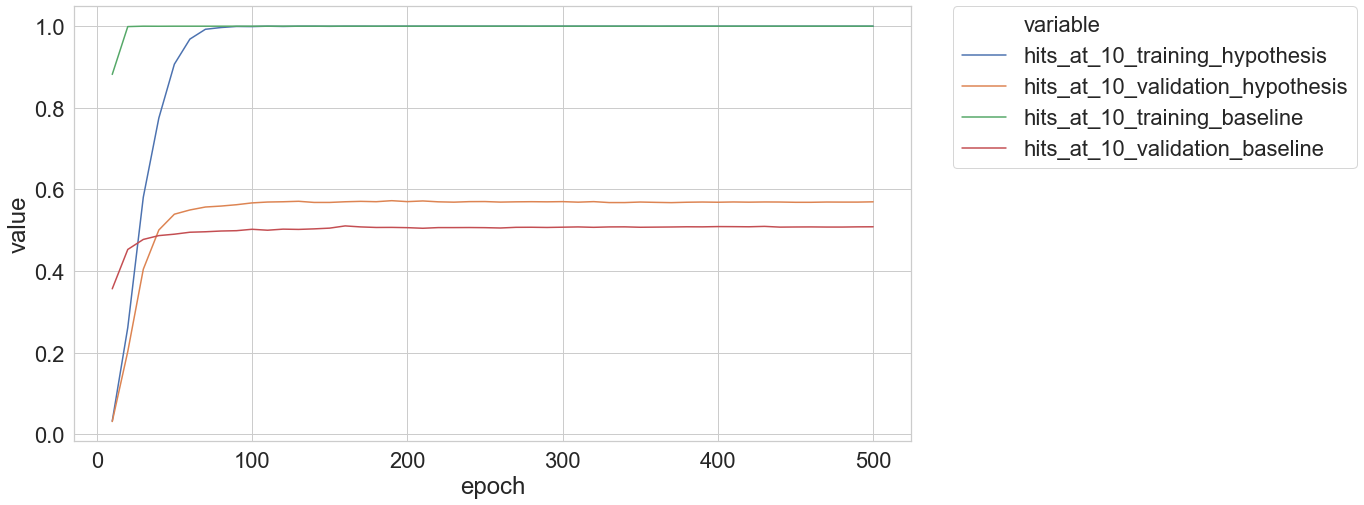
\includegraphics[width=1.0\linewidth, height=0.5\linewidth]{WN18RR_hits_at_10_Results_ptwv}
		\captionsetup{justification=centering}
		\caption{WN18RR: HypER+ vs \\ HypER+ with pre-trained embeddings}
	\end{subfigure}
	\begin{subfigure}[b]{.5\linewidth}
   		\centering
		\includegraphics[width=1.0\linewidth, height=0.5\linewidth]{FB15k-237_hits_at_10_Results_ptwv}
		\captionsetup{justification=centering}
		\caption{FB15k-237: HypER+ vs \\ HypER+ with pre-trained embeddings}
	\end{subfigure}
	\captionsetup{justification=centering}
	\caption{Hit@10 vs training epoch. The hypothesis significantly outperforms the baseline on the WN18RR KG. The hypothesis only marginally outperforms the baseline on the FB15k-237 KG. This suggests pre-trained embeddings have more of an impact on smaller KGs, where relations are likely to be more sparse, making it harder to build entity and relation conceptual understanding.}
\end{figure}


%********************************** %Mean rank **************************************

\begin{figure}
	\begin{subfigure}[b]{.5\linewidth}
   		\centering
    		\includegraphics[width=1.0\linewidth, height=0.6\linewidth]{WN18RR_mean_rank_Results_ptwv}
		\captionsetup{justification=centering}
		\caption{WN18RR: HypER+ vs \\ HypER+ with pre-trained embeddings}
	\end{subfigure}
	\begin{subfigure}[b]{.5\linewidth}
   		\centering
		\includegraphics[width=1.0\linewidth, height=0.6\linewidth]{FB15k-237_mean_rank_Results_ptwv}
		\captionsetup{justification=centering}
		\caption{FB15k-237: HypER+ vs \\ HypER+ with pre-trained embeddings}
	\end{subfigure}
	\captionsetup{justification=centering, name={Figure}}
	\caption{Mean Rank vs training epoch. There is a stark difference in performance between the hypothesis and baseline on the WN18RR KG. Pre-trained embeddings are very effective at providing semantic information that can be used to produce good predictions for smaller, less complex KGs. The difference is less pronounced on the FB15k-237 KG, however is still significant.}
\end{figure}


%********************************** %Test results **************************************

\begin{table}
		\centering
		\begin{tabular}{lllllllllll}
  			\textbf{Model} & \textbf{H@10} & \textbf{H@3} & \textbf{H@1} & \textbf{MR} & \textbf{MRR} \\
  			\hline
  			DistMult \unskip~\citep{yang2014embedding} & .490 & .440 & .390 & 5110 & .430 \\
  			ComplEx \unskip~\citep{trouillon2016complex} & .510 & .460 & .410 & 5261 & .440 \\
  			Neural LP \unskip~\citep{yang2017differentiable} & - & - & - & - & - \\
			ConvE \unskip~\citep{dettmers2018convolutional} & .520 & .440 & .400 & 4187 & .430 \\
			HypER \unskip~\citep{balazevic2019hypernetwork} & .522 & .477 & .436 & 5798 & .465 \\
			HypER+ (ours) & .519 & .479 & \textbf{.438} & 7061 & .466 \\
  			\hline
  			HypER+ with pre-trained embeddings (ours) & \textbf{.578} & \textbf{.493} & .435 & \textbf{1063} & \textbf{.480} \\
			&
		\end{tabular}
		\captionsetup{justification=centering}
		\caption{Relation prediction test results on WN18RR. HypER+ with pre-trained word embeddings significantly outperforms both the HypER as well as HypER+ models. HypER+ outperforms HypER+ with pre-trained embeddings on the Hit@1 metric, consistent with the expectation of diminished impact of pre-trained embeddings at high levels of accuracy constraints. It should be noted that there is a difference of $ 0.3 \% $ between all three models (HypER, HypER+ and HypER+ with pre-trained word embeddings), suggesting almost identical performance. The largest differences in performance occur at Hit@10 and Mean Rank, bearing the effectiveness of pre-trained embeddings at compensating for sparsity, however also highlighting how their significance diminishes at higher levels of accuracy. }
\end{table}

\begin{table}
		\centering
		\begin{tabular}{lllllllllll}
  			\textbf{Model} & \textbf{H@10} & \textbf{H@3} & \textbf{H@1} & \textbf{MR} & \textbf{MRR} \\
  			\hline
  			DistMult \unskip~\citep{yang2014embedding} & .419 & .263 & .155 & 254 & .241 \\
  			ComplEx \unskip~\citep{trouillon2016complex} & .428 & .275 & .158 & 339 & .247 \\
  			Neural LP  \unskip~\citep{yang2017differentiable} & .408 & - & - & - & .250 \\
			ConvE \unskip~\citep{dettmers2018convolutional} & .501 & .356 & .237 & 244 & .325 \\
			HypER \unskip~\citep{balazevic2019hypernetwork} & .520 & .376 & .252 & 250 & .341 \\
			HypER+ (ours) & .516 & .368 & .245 & 268 & .335 \\
  			\hline
  			HypER+ with pre-trained embeddings (ours) & \textbf{.525} & \textbf{.379} & \textbf{.255} & \textbf{196} & \textbf{.345} \\
			&
		\end{tabular}
		\captionsetup{justification=centering}
		\caption{Relation prediction test results on FB15k-237. The HypER+ model with pre-trained embeddings achieves state-of-the-art performance across all metrics. Covariate shift seems to not be playing as meaningful a role, and pre-trained embeddings are providing a more meaningful contribution, as suggested by the HypER+ model's inferior performance to the HypER model. Strangely, this is inconsistent with training and validation set results, where HypER+ consistently outperforms HypER on FB15k-237. The fact that we use the quoted HypER test results, as opposed to reimplemented and verified test results, may explain this inconsistency. This inconsistency aside, pre-trained embeddings remain effective at improving relation prediction performance on the FB15k-237 KG.}
\end{table}


%********************************** %Test Result Decomposition **************************************

\begin{figure} [H]
   	\centering
    	\includegraphics[width=0.7\textwidth, height=0.3\textheight]{WN18RR_relational_performance_results}
	\captionsetup{justification=centering}
	\caption{WN18RR Hit@1 predicate performance of the HypER+ model with pre-trained embeddings. The model performs well with synonym relation types, but performs poorly with compositional and hierarchical relations. This may be due to the inherent similarity and analogy in concepts, whereas compositions and hierarchies can be defined by strict rules. Perhaps, more simply, it could be due to the number of test set samples for each relation, where higher numbers increase the prediction error rate.}
\end{figure}

\bigskip
\bigskip
\bigskip
\bigskip

\begin{table}[H]
	\centering
	\resizebox{1.0\columnwidth}{!}{
	\begin{tabular}{lllllllllll}
  		\textbf{Subject} & \textbf{Predicate} & \textbf{Object Target} & \textbf{Object Prediction} \\
  		\hline
  		usa & has part & colorado & missouri river \\
  		spain & has part & cadiz & jerez de la frontera \\
  		kilobyte & has part & computer memory unit & word \\
		electromagnetic spectrum & has part & actinic ray & radio spectrum \\
		systema respiratorium & has part & respiratory tract & respiratory organ \\
		respiratory organ & has part & nsa & defense advanced research projects agency \\
		africa & has part & nigeria & senegal \\
  		antigen & has part & substance & epitope \\
		amphitheatre & has part & theatre & tiered seat \\
		indian ocean & has part & mauritius & antarctic ocean \\
		&
	\end{tabular}
	}
	\captionsetup{justification=centering}
	\caption{Qualitative Hit@1 test results on WN18RR. The table presents a set of questions posed to the HypER+ with pre-trained embeddings model. "Object Target" is the expected answer, and "Object Prediction" is the answer given by the model. The model demonstrates basic conceptual understanding, never making mistakes that would be considered obvious by humans. We would expect reasonable knowledge discovery utility from the model, when used jointly with information retrieval for open-domain question answering \unskip~\citep{chen2017reading}. }
\end{table}


%********************************** %Chapter Summary  **************************************

\section{Summary}

\textbf{NTN with optimised training algorithm.}\ We attempted to improve the NTN model by applying training algorithm optimisations including early stopping, the Adam optimiser and hyperparameter random search. The results indicate that there are potential performance gains to be realised simply through using training algorithm techniques known to improve performance. In this instance we see an accuracy gain of 6.2\% across the WordNet and Freebase datasets. \par

\noindent \textbf{HypER+.}\ We compensated for possible covariate shift introduced by hypernetworks.\ The latent representation distribution drift of relations is pronounced enough that we are able to improve the Hit@1 accuracy of the original HypER model on average by 2.7\%, across the WN18 and FB15k KGs.\ We note graph modelling may be a worthwhile paradigm to explore for link prediction, given R-GCN's SOTA performance for Hit@10 accuracy on the WN18 KG. We also note the greater influence of relational normalisation on prediction performance for larger and more complex KGs. \par

\noindent \textbf{HypER+ with pre-trained word vectors.}\ Finally we extended HypER+ to make use of pre-trained GloVe word vectors.\ The semantic information inherent in these embeddings significantly improves relation prediction performance on sparse relational data. Their influence is somewhat reduced at higher levels of accuracy, where KG domain alignment becomes more important. Pre-trained word vectors also offer less utility for large and complex KGs, however still contribute an improvement to prediction. The combination of relation normalisation, and entity and relation embedding initialisation using pre-trained word vectors, both addresses the problems of data sparsity, as well as produces higher quality relational latent representations for large and complex datasets. As a result, HypER+ with pre-trained word vectors achieves SOTA performance on almost all standard link prediction benchmark metrics, across the challenging WN18RR and FB15k-237 KGs. 

%%!TEX root = ../thesis.tex
%*******************************************************************************
%*********************************** Fifth Chapter *****************************
%*******************************************************************************

\ifpdf
     \graphicspath{{/Users/luyolomagangane/Documents/Academics/Figures/Chapter5/}}
\else
    \graphicspath{{Chapter1/Figs/Vector/}{Chapter1/Figs/}}
\fi

\chapter{Results and Analysis}  %Title of the Fifth Chapter

\section{Nonlinear Tensor Factorisation}
% Background on 3 hypotheses that were tested
\subsubsection{Overview}
This chapter explores three hypotheses explored for link prediction using knowledge graph nonlinear tensor factroisation, namely the application of best practise deep learning techniques to recursive neural tensor networks, relational filter regularisation using dropout in hyper convolutional neural tensor networks, and finally the application of pretrained word embeddings in hyper convolutional neural tensor factorisation. \newline 

Tensor factorisation is the use of high dimensional tensors for relational modeling ~\citep{Nickel_2016}. Statistical relational learning has traditionally relied on linear modelling techniques in order to constrain parameterisation for computational efficiency at the expense of model expressiveness i.e. models that suffer from high bias. Recently nonlinear approaches have been proposed to overcome the bias problem and each propose hypothesis that aim to take advantage of their distinct architecture. The first nonlinear model to gain surpass state-of-the-art tensor factorisation models, was the recursive neural tensor network \cite{refefence}. There are two hypotheses proposed that were proposed in using this model architecture for link prediction, namely that recursive architectures are useful in part of speech tagging \cite{reference}, as the perform a combinatorial analysis of word sequences in sentences, instead of the conventional linear sequence used in part of speech tagging \cite{reference}. The second hypothesis is that pre-trained word embeddings offer superior performance to randomly generated entity vectors which were commonly used at the time for tensor factorisation \cite{reference}. \newline
The second hypothesis we explored is the use of convolutional hyper networks with relational factorisation for link prediction \cite{reference}. This research is the current state-of-that-art latent feature modelling technique for link prediction \cite{reference}. There are also two hypotheses explored in this research - the first is that convolutional filters can be used explicitly for relational factorisation \cite{reference}, the second is that the hyper network architecture is useful in generating the relational filters due to increased parameterisation using a hyper linear layer \cite{reference}. \newline
The final hypothesis we explored is the use of contextual entity representations as input to convolutional hyper networks. State-of-the-art natural language modelling techniques makes use contextual word representations \cite{Elmo, Bert} instead of static word embeddings \cite{fasttext, GloVe, Word2Vec}. Contextual word embeddings are represented as distinct subject entity representations, and distinct object entity representations. \newline
The following chapter presents the results and analysis from the experiments performed to validate these hypotheses.

\section{Recursive Neural Tensor Networks}
\subsubsection{Model Summary} 
Tensor factorisation has been a popular approach applied to statistical relational learning (SRL) \cite{reference, reference, reference}. In order to improve model expressiveness, a Recursive Neural Tensor Network architecture was proposed \cite{reference}. This model is inspired by recursive neural networks \cite{reference}. Recursive neural networks have been applied to natural language processing tasks, particularly part of speech tagging \cite{reference}. Traditionally, recurrent neural networks have been applied to this task \cite{reference}. Recurrent neural networks are based on the Markov assumption \cite{reference}, where the future states of the process depends only on the present state, not on the sequence of events that preceded it \cite{reference}. The state is constructed using sequential input within a time step window, for example, a sentence will contain a sequence of words, and the window will be the last word in the sentence and the four previous words before an anchor word. The state consists of the four previous words before the anchor word, and along with the anchor word, can be used to predict the next word in the sequence.\newline
Instead of producing a state using a sequence of previous words, recursive neural networks generate the state using a combinatorial tree of the word sequence. The number of potential combinations are dependent on the length of the sequence, for example a three word sequence has three combinations, a four word sequence has six combinations and  a five word sequence has ten combinations. The combinations which produce the smallest magnitudes are then filtered out from the network, and remaining combinations are then recombined as new combinations, This filtering and recombination process is then continued until a next word prediction is made. \newline
Recursive neural networks are combined with tensor factorisation to produce a more expressive model for link prediction. The subject and object entities are concatenated and then an matrix multiplication is taken with the resultant vector before a bias is added. \newline
\subsubsection{Contrastive Max Margin Loss}
The contrastive max-magrin loss \cite{reference} is used to train the RTNT model. The input consists of an entity-relational pair, where the entity is a subject entity. An object entity is presented as a target to complete the triple. A non-related object entity is presented is then presented as a corrupt object entity. Fact score is then computed for the target triple, as well as the corrupt triple as logits, and the difference between the two logits is the contrast between the true and false facts. The task is for the model is then to produce a higher fact score for the true triple than the false triple. If the model gets it wrong, then loss is generated and back propagated through the network to update model parameters. \newline

\subsubsection{Experimental Setup} 

We use the following benchmark knowledge graphs: Wordnet - a lexical database for English, it is a taxonomy with hypernyms (is-a) relationships, and synonym sets. \newline
Freebase - a large collaborative knowledge base consisting of data about the world composed mainly by its community members. It was an online collection of structured data harvested from many sources, including user-submitted wiki contributions. \newline
Visualisations of the respective knowledge graphs are presented below:

\begin{figure}[H]
  	\caption{Wordnet Entities and Relations Graphplot}
   	\centering
    	\includegraphics[width=\textwidth]{Wordnet}
\end{figure}

\begin{figure}[H]
  	\caption{Freebase Entity and Relations Graphplot}
   	\centering
    	\includegraphics[width=\textwidth]{Freebase}
\end{figure}


We used the Tensorflow framework to develop our model.  This model is built on top of the Neural Tensor model introduced by (Socher, Chen, Manning and Ng 2013) ~\citep{NIPS2013_5028} and implemented in Tensorflow by (Doss, LeNail and Liu 2015)  ~\citep{Doss2015}. Randomly initialised entity and relational embeddings are used to initialise model training. These embeddings are dynamically adjusted during the training process to generate latent representations specific to the knowledge domain. Property counts for the respective knowledge graphs are presented below:

\begin{figure}[H]
	\parbox{.5\linewidth}{
   		\caption{Wordnet Property Barplot}
   		\centering
    		\includegraphics[width=0.45\textwidth]{Wordnet_Counts}
		}
	\hfill
	\parbox{.5\linewidth}{
		\caption{Freebase Property Barplot}
   		\centering
    		\includegraphics[width=0.45\textwidth]{Freebase_Counts}
		}
\end{figure}


\begin{table}[H]
	\parbox{.5\linewidth}{
		\caption{Wordnet Property Counts}
		\centering
		\begin{tabular}{lllllllllll}
  			\textbf{Property} & \textbf{Count}  \\
  			\hline
  			Entities & 38,696  \\
  			Relations & 11  \\
  			Triples & 136,611  \\
		\end{tabular}
		}
	\hfill
	\parbox{.5\linewidth}{
		\caption{Freebase Property Counts}
		\centering
		\begin{tabular}{lllllllllll}
  			\textbf{Property} & \textbf{Count}  \\
  			\hline
  			Entities & 75,043   \\
  			Relations & 13  \\
  			Triples & 375,499  \\
		\end{tabular}
		}
\end{table}


Summary statistics of the respective knowledge graphs Resource Description Framework (RDF) decomposition - subject, predicate, object - are presented below:

% Predicate

\begin{figure}[H]
	\parbox{.5\linewidth}{
   		\caption{Wordnet Predicate Barplot}
   		\centering
    		\includegraphics[width=0.45\textwidth, height=0.2\textheight]{Wordnet_Predicate_Counts}
		}
	\hfill
	\parbox{.5\linewidth}{
		\caption{Freebase Predicate Barplot}
   		\centering
		\includegraphics[width=0.45\textwidth, height=0.2\textheight]{Freebase_Predicate_Counts}
		}
\end{figure}

\begin{table}[H]
	\parbox{.5\linewidth}{
		\caption{Wordnet Predicate Statistics}
		\centering
		\begin{tabular}{lllllllllll}
  			\textbf{Statistic} & \textbf{Value}  \\
  			\hline
			Count & 11 \\
			Max & 43,312  \\
			Min & 1,229  \\
  			Median & 7,705  \\
  			IQR & 7,257.5  \\
		\end{tabular}
		}
	\hfill
	\parbox{.5\linewidth}{
		\caption{Freebase Predicate Statistics}
		\centering
		\begin{tabular}{lllllllllll}
  			\textbf{Statistic} & \textbf{Value}  \\
  			\hline
			Count & 13 \\
			Max & 73,897  \\
			Min & 4, 464  \\
  			Median & 21,149  \\
  			IQR & 34,033  \\
		\end{tabular}
		}
\end{table}

% Subject

\begin{figure}[H]
	\parbox{.5\linewidth}{
   		\caption{Wordnet Subject Barplot}
   		\centering
    		\includegraphics[width=0.45\textwidth, height=0.2\textheight]{Wordnet_Subject_Counts}
		}
	\hfill
	\parbox{.5\linewidth}{
		\caption{Freebase Subject Barplot}
   		\centering
		\includegraphics[width=0.45\textwidth, height=0.2\textheight]{Freebase_Subject_Counts}
		}
\end{figure}


\begin{table}[H]
	\parbox{.5\linewidth}{
		\caption{Wordnet Subject Statistics}
		\centering
		\begin{tabular}{lllllllllll}
  			\textbf{Statistic} & \textbf{Value}  \\
  			\hline
			Count & 32,720 \\
			Max & 619 \\
			Min & 1 \\
  			Median & 2 \\
  			IQR & 2 \\
		\end{tabular}
		}
	\hfill
	\parbox{.5\linewidth}{
		\caption{Freebase Subject Statistics}
		\centering
		\begin{tabular}{lllllllllll}
  			\textbf{Statistic} & \textbf{Value}  \\
  			\hline
			Count & 67,393 \\
			Max & 37 \\
			Min & 1 \\
  			Median & 5 \\
  			IQR & 4 \\
		\end{tabular}
		}
\end{table}

% Object

\begin{figure}[H]
	\parbox{.5\linewidth}{
   		\caption{Wordnet Object Barplot}
   		\centering
    		\includegraphics[width=0.45\textwidth, height=0.2\textheight]{Wordnet_Object_Counts}
		}
	\hfill
	\parbox{.5\linewidth}{
		\caption{Freebase Object Barplot}
   		\centering
		\includegraphics[width=0.45\textwidth, height=0.2\textheight]{Freebase_Object_Counts}
		}
\end{figure}


\begin{table}[H]
	\parbox{.5\linewidth}{
		\caption{Wordnet Object Statistics}
		\centering
		\begin{tabular}{lllllllllll}
  			\textbf{Statistic} & \textbf{Value}  \\
  			\hline
			Count & 33,011 \\
			Max & 537 \\
			Min & 1 \\
  			Median & 3 \\
  			IQR & 2 \\
		\end{tabular}
		}
	\hfill
	\parbox{.5\linewidth}{
		\caption{Freebase Object Statistics}
		\centering
		\begin{tabular}{lllllllllll}
  			\textbf{Statistic} & \textbf{Value}  \\
  			\hline
			Count & 15,342 \\
			Max & 59,663 \\
			Min & 1 \\
  			Median & 3 \\
  			IQR & 6 \\
		\end{tabular}
		}
\end{table}

For Wordnet, it can be seen that relations are skewed toward "has instance" 43,312 occurrences, and "type of" 36,659 occurrences. We would expect poor performance from the model for out-of-sample data containing
containing relations that are not "has instance" or "type of". Freebase relations are somewhat more uniform, however four relations have occurrences under 10,000. We would expect reasonable performance across all relations for this knowledge graph. \newline
Wordnet and Freebae subjects are somewhat uniform, although the median number of occurrences is 2 and 5 respectively, with an IQR of 2 and 4 respectively. This are thus sparse distributions of data points, and the model will need to rely on 
similarity of subject features in order to produce sensible inference. \newline
Wordnet object occurrences are somewhat uniform. Freebase object occurrences are skewed, with a single object, "male" occurring 59,663 times, representing 15,88\% of facts. This is in comparison to a median object occurrence of 3 and an interquartile range of 6.
We would expect poor performance from a Freebase link prediction model given this distribution of objects. \newline

% Best Practise Deep Learning Techniques

\subsubsection{Hypothesis 1: \newline 
Recursive Neural Tensor Networks with Best Practise Deep Learning Techniques}
Model hyperparameter optimisation is implemented using random grid search. The the model was trained on a MacBook Pro 2015 with 8 cores, 16GB RAM, and 512GB SSD. \newline
We evaluate the model by ranking the accuracy scores of the predicted triples for the respective datasets. Code to reproduce: https://github.com/xhosaBoy/deep-knowledge-modelling

\subsubsection{Batching, Logits and Early Stopping}
Machine learning models can suffer from overfitting \cite{reference} - when training has progressed too long, and the model parameters have been optimised for prediction on the training set. This leads to poor generalisation  and reveals itself in the form of increasing training accuracy, and decreasing validation accuracy. In order to overcome this problem, early stopping is often used during training. This is when triaining is terminated should decreasing validation accuracy be detected.\newline

\subsubsection{Link Prediction Results}
The link prediction accuracy results of the RNTN model, a nonlinear factorisation model compared against linear factorisation models, are presented in table 5.1:

\begin{figure}[H]
	\parbox{.5\linewidth}{
   		\caption{Wordnet Cost}
   		\centering
    		\includegraphics[width=0.45\textwidth, height=0.2\textheight]{Wordnet_Cost_Results_Early_Stopping}
		}
	\hfill
	\parbox{.5\linewidth}{
		\caption{Freebase Cost}
   		\centering
		\includegraphics[width=0.45\textwidth, height=0.2\textheight]{Freebase_Cost_Results}
		}
\end{figure}


\begin{figure}[H]
	\parbox{.5\linewidth}{
   		\caption{Wordnet Accuracy}
   		\centering
    		\includegraphics[width=0.45\textwidth, height=0.2\textheight]{Wordnet_Accuracy_Results_Early_Stopping}
		}
	\hfill
	\parbox{.5\linewidth}{
		\caption{Freebase Accuracy}
   		\centering
		\includegraphics[width=0.45\textwidth, height=0.2\textheight]{Freebase_Accuracy_Results}
		}
\end{figure}



\begin{table}[H]
	\caption{Link prediction accuracy on Wordnet and Freebase}
	\centering
	\begin{tabular}{lllllllllll}
  		\textbf{Model} & \textbf{Wordnet} & \textbf{Freebbase} & \textbf{Avg} \\
  		\hline
  		Distance Model & .683 & .610 & .647 \\
  		Hadamard Model & .800 & .688 & .744 \\
  		Single Layer Model & .760 & .853 & .807 \\
  		Bilinear Model & \textbf{.841} & \textbf{.877} & \textbf{.859} \\
  		Recursive Neural Tensor Network & .562 & .535 & .549 \\
  		\hline
  		Recursive Neural Tensor Network+ & .674 & .548 & .611 \\
	\end{tabular}
\end{table}

\section{HypER Convolutional Neural Networks}

\subsubsection{Model Summary} 
In order to overcome the expressiveness problems evident in the Freebase test dataset, more nonlinear relational factorisation approaches have been proposed \cite{ComplEx, Neural LP, TorusE}. \newline
HypER is a model that uses convolutional relational filters r that are convolved with the subject entity e1, producing an intermediate relational representation. The dot product of the relational representation is then taken with the object entity e2 to produce relation-specific score between the two entities. The HypER model only produces a latent relational representation for the subject entity e1, we extend this model to also produce a relational representation for the object entity e2, and call this model HpyER+. HypER+ thus produces entity-relational representations that approximate KG spacial locality. \newline
\subsubsection{Binary Cross Entropy Loss}
The binary cross entropy loss \cite{reference} is used to train the HypER Convolutional model. Like the RNTN model, the input consists of an entity-relational pair, where the entity is a subject entity and an object entity is presented as a target to complete the triple. A logit is generated for each sample and passed through through a logarithmic sigmoid or softmax function. Loss is generated by comparing the produced likelihood with the expected likelihood, 0 or 1. The sum of all losses is aggregated and back propagated through the network for parameter update. \newline

\subsubsection{Experimental Setup} 

We use the following benchmark knowledge graphs: WN18 (Bordes et al. 2013) is a subset of Wordnet, a database containing lexical relations between words. The knowledge graph contains 40,943 entities and 18 relations. \newline 
FB15k - (Bordes et al. 2013) is a subset of Freebase, a large database of facts about the real world. FB15k contains 14,951 entities and 1,345 relations. \newline \newline
Visualisations of the respective knowledge graphs are presented below:

\begin{figure}[H]
  	\caption{WN18 Entities and Relations Graphplot}
   	\centering
    	\includegraphics[width=\textwidth]{WN18_Graph}
\end{figure}

\begin{figure}[H]
  	\caption{FB15k Entity and Relations Graphplot}
   	\centering
    	\includegraphics[width=\textwidth]{FB15k_Graph}
\end{figure}


We used the Pytorch framework to develop our model. This model is built on top of the HypER model introduced by (Balaˇzevi´c, Allen, and Hospedales 2018) ~\citep{balazevic2019hypernetwork}.  Randomly initialised entity and relational embeddings are used to initialise model training. These embeddings are dynamically adjusted during the training process to generate latent representations specific to the knowledge domain. Property counts for the respective knowledge graphs are presented below:

\begin{figure}[H]
	\parbox{.5\linewidth}{
   		\caption{WN18 Property Barplot}
   		\centering
    		\includegraphics[width=0.45\textwidth]{WN18_Counts}
		}
	\hfill
	\parbox{.5\linewidth}{
		\caption{FB15k Property Barplot}
   		\centering
    		\includegraphics[width=0.45\textwidth]{FB15k_Counts}
		}
\end{figure}


\begin{table}[H]
	\parbox{.5\linewidth}{
		\caption{WN18 Property Counts}
		\centering
		\begin{tabular}{lllllllllll}
  			\textbf{Property} & \textbf{Count}  \\
  			\hline
  			Entities & 40,943  \\
  			Relations & 18  \\
  			Triples & 151,442 \\
		\end{tabular}
		}
	\hfill
	\parbox{.5\linewidth}{
		\caption{FB15k Property Counts}
		\centering
		\begin{tabular}{lllllllllll}
  			\textbf{Property} & \textbf{Count}  \\
  			\hline
  			Entities & 14,951   \\
  			Relations & 1,345  \\
  			Triples & 592,213  \\
		\end{tabular}
		}
\end{table}


Summary statistics of the respective knowledge graphs Resource Description Framework (RDF) decomposition - subject, predicate, object - are presented below:

% Predicate

\begin{figure}[H]
	\parbox{.5\linewidth}{
   		\caption{WN18 Predicate Barplot}
   		\centering
    		\includegraphics[width=0.45\textwidth, height=0.2\textheight]{WN18_Predicate_Counts}
		}
	\hfill
	\parbox{.5\linewidth}{
		\caption{FB15k Predicate Barplot}
   		\centering
		\includegraphics[width=0.45\textwidth, height=0.2\textheight]{FB15k_Predicate_Counts}
		}
\end{figure}

\begin{table}[H]
	\parbox{.5\linewidth}{
		\caption{WN18 Predicate Statistics}
		\centering
		\begin{tabular}{lllllllllll}
  			\textbf{Statistic} & \textbf{Value}  \\
  			\hline
			Count & 18 \\
			Max & 37,221  \\
			Min & 86 \\
  			Median & 3,242.5  \\
  			IQR & 6,190.75  \\
		\end{tabular}
		}
	\hfill
	\parbox{.5\linewidth}{
		\caption{FB15k Predicate Statistics}
		\centering
		\begin{tabular}{lllllllllll}
  			\textbf{Statistic} & \textbf{Value}  \\
  			\hline
			Count & 1,345 \\
			Max & 19,764  \\
			Min & 1  \\
  			Median & 26  \\
  			IQR & 166  \\
		\end{tabular}
		}
\end{table}

% Subject

\begin{figure}[H]
	\parbox{.5\linewidth}{
   		\caption{WN18 Subject Barplot}
   		\centering
    		\includegraphics[width=0.45\textwidth, height=0.2\textheight]{WN18_Subject_Counts}
		}
	\hfill
	\parbox{.5\linewidth}{
		\caption{FB15k Subject Barplot}
   		\centering
		\includegraphics[width=0.45\textwidth, height=0.2\textheight]{FB15k_Subject_Counts}
		}
\end{figure}


\begin{table}[H]
	\parbox{.5\linewidth}{
		\caption{WN18 Subject Statistics}
		\centering
		\begin{tabular}{lllllllllll}
  			\textbf{Statistic} & \textbf{Value}  \\
  			\hline
			Count & 32,544 \\
			Max & 520 \\
			Min & 1 \\
  			Median & 3 \\
  			IQR & 2 \\
		\end{tabular}
		}
	\hfill
	\parbox{.5\linewidth}{
		\caption{FB15k Subject Statistics}
		\centering
		\begin{tabular}{lllllllllll}
  			\textbf{Statistic} & \textbf{Value}  \\
  			\hline
			Count &14,865 \\
			Max & 4,381 \\
			Min & 1 \\
  			Median & 27 \\
  			IQR & 32 \\
		\end{tabular}
		}
\end{table}

% Object

\begin{figure}[H]
	\parbox{.5\linewidth}{
   		\caption{WN18 Object Barplot}
   		\centering
    		\includegraphics[width=0.45\textwidth, height=0.2\textheight]{WN18_Object_Counts}
		}
	\hfill
	\parbox{.5\linewidth}{
		\caption{FB15k Object Barplot}
   		\centering
		\includegraphics[width=0.45\textwidth, height=0.2\textheight]{FB15k_Object_Counts}
		}
\end{figure}


\begin{table}[H]
	\parbox{.5\linewidth}{
		\caption{WN18 Object Statistics}
		\centering
		\begin{tabular}{lllllllllll}
  			\textbf{Statistic} & \textbf{Value}  \\
  			\hline
			Count & 32,543 \\
			Max & 520 \\
			Min & 1 \\
  			Median & 3 \\
  			IQR & 2 \\
		\end{tabular}
		}
	\hfill
	\parbox{.5\linewidth}{
		\caption{FB15k Object Statistics}
		\centering
		\begin{tabular}{lllllllllll}
  			\textbf{Statistic} & \textbf{Value}  \\
  			\hline
			Count & 14,930 \\
			Max & 9,645 \\
			Min & 1 \\
  			Median & 23 \\
  			IQR & 30 \\
		\end{tabular}
		}
\end{table}

For WN18, it can be seen that relations are skewed toward the relations "hyponym",  "hypernym", and "derivationally related from", with a maximum of 37,221 occurrences. \newline
FB15k relations are somewhat more uniform. We would expect reasonable performance across all relations for this knowledge graph. \newline
WN18 and FB15k subjects are somewhat uniform aside from a small number of high occurrences entities, with the median number of occurrences is 3 and 27 respectively, and with an IQR of 2 and 32 respectively. 
WN18 object occurrences are somewhat uniform. FB15k object occurrences are skewed, with the "United States" partaking in the highest number of facts. This is in comparison to a median object occurrence of 3 and an interquartile range of 23.

%  Regularised Relational Filters

\subsubsection{Hypothesis 2: \newline 
HypER Relational Filter Regularisation: HypER+}
HypER Relational Filter Regularisation, introduced as HypER+, is implemented using regularised relational filters, as well an adjustment of hidden layer regularisation, from the original HypER model. \newline
The the model was trained on Google Cloud Platform, on a N1 series instance with  8 CPU cores, 30GB RAM, 512GB SSD and a Nvidia Tesla P100 GPU. \newline
We evaluate the model using standard link prediction benchmarks. \newline 
Code to reproduce: https://github.com/xhosaBoy/HypER-Regularised-Relations \newline
Baseline: https://github.com/xhosaBoy/HypER-baseline

\subsubsection{Dropout and Batch Normalisation}
Deep learning models are prone to overfitting training data due to over parameterisation ~\citep{dropout paper}. A technique called dropout is used to overcome this problem. 
Dropout involves removing nodes within a layer, to remove excessive dependency on that node by the model. This encourages generalisation by the model, to the underlying distribution of the data. \newline  
Datasets often suffer from noise. This noise masks the true underlying distribution of the data, and can make it challenging for a model to estimate the likely distribution.
An aggregation of data samples help reveal the true distribution ~\citep{Book about statistical machine learning}. Batch nomralisation is the application of statistical properties of such a data aggregation
to individual data points within a dataset. Typically the mean and standard deviation of the bath is applied to a batch that will be used to compute forward and back propagation through the network. \newline
This technique is applied to relational filters in the HypER model. Batch normalisaiton is already applied to entity data points in the model. 

\subsubsection{Link Prediction Results}
The link prediction benchmark results of the HypER+ model, compared against other link prediction models, are presented below:

% Cost

\begin{figure}[H]
	\parbox{.5\linewidth}{
   		\caption{WN18 Cost}
   		\centering
    		\includegraphics[width=0.45\textwidth, height=0.2\textheight]{WN18_Cost_Results}
		}
	\hfill
	\parbox{.5\linewidth}{
		\caption{FB15k Cost}
   		\centering
		\includegraphics[width=0.45\textwidth, height=0.2\textheight]{FB15k_Cost_Results}
		}
\end{figure}

\begin{figure}[H]
	\parbox{.5\linewidth}{
   		\caption{WN18 Cost Clipped View}
   		\centering
    		\includegraphics[width=0.45\textwidth, height=0.2\textheight]{WN18_Cost_Results_Clipped}
		}
	\hfill
	\parbox{.5\linewidth}{
		\caption{FB15k Cost Clipped View}
   		\centering
		\includegraphics[width=0.45\textwidth, height=0.2\textheight]{FB15k_Cost_Results_Clipped}
		}
\end{figure}

% Hits@10

\begin{figure}[H]
	\parbox{.5\linewidth}{
   		\caption{WN18 Hits@10}
   		\centering
    		\includegraphics[width=0.45\textwidth, height=0.2\textheight]{WN18_hits_at_10_Results}
		}
	\hfill
	\parbox{.5\linewidth}{
		\caption{FB15k Hits@10}
   		\centering
		\includegraphics[width=0.45\textwidth, height=0.2\textheight]{FB15k_hits_at_10_Results}
		}
\end{figure}

\begin{figure}[H]
	\parbox{.5\linewidth}{
   		\caption{WN18 Hits@10 Clipped View}
   		\centering
    		\includegraphics[width=0.45\textwidth, height=0.2\textheight]{WN18_hits_at_10_Results_Clipped}
		}
	\hfill
	\parbox{.5\linewidth}{
		\caption{FB15k Hits@10  Clipped View}
   		\centering
		\includegraphics[width=0.45\textwidth, height=0.2\textheight]{FB15k_hits_at_10_Results_Clipped}
		}
\end{figure}

% Hits@3

\begin{figure}[H]
	\parbox{.5\linewidth}{
   		\caption{WN18 Hits@3}
   		\centering
    		\includegraphics[width=0.45\textwidth, height=0.2\textheight]{WN18_hits_at_3_Results}
		}
	\hfill
	\parbox{.5\linewidth}{
		\caption{FB15k Hits@3}
   		\centering
		\includegraphics[width=0.45\textwidth, height=0.2\textheight]{FB15k_hits_at_3_Results}
		}
\end{figure}

\begin{figure}[H]
	\parbox{.5\linewidth}{
   		\caption{WN18 Hits@3 Clipped View}
   		\centering
    		\includegraphics[width=0.45\textwidth, height=0.2\textheight]{WN18_hits_at_3_Results_Clipped}
		}
	\hfill
	\parbox{.5\linewidth}{
		\caption{FB15k Hits@3  Clipped View}
   		\centering
		\includegraphics[width=0.45\textwidth, height=0.2\textheight]{FB15k_hits_at_3_Results_Clipped}
		}
\end{figure}

% Hits@1

\begin{figure}[H]
	\parbox{.5\linewidth}{
   		\caption{WN18 Hits@1}
   		\centering
    		\includegraphics[width=0.45\textwidth, height=0.2\textheight]{WN18_hits_at_1_Results}
		}
	\hfill
	\parbox{.5\linewidth}{
		\caption{FB15k Hits@1}
   		\centering
		\includegraphics[width=0.45\textwidth, height=0.2\textheight]{FB15k_hits_at_1_Results}
		}
\end{figure}

\begin{figure}[H]
	\parbox{.5\linewidth}{
   		\caption{WN18 Hits@1 Clipped View}
   		\centering
    		\includegraphics[width=0.45\textwidth, height=0.2\textheight]{WN18_hits_at_1_Results_Clipped}
		}
	\hfill
	\parbox{.5\linewidth}{
		\caption{FB15k Hits@1  Clipped View}
   		\centering
		\includegraphics[width=0.45\textwidth, height=0.2\textheight]{FB15k_hits_at_1_Results_Clipped}
		}
\end{figure}

% Mean rank

\begin{figure}[H]
	\parbox{.5\linewidth}{
   		\caption{WN18 Mean Rank}
   		\centering
    		\includegraphics[width=0.45\textwidth, height=0.2\textheight]{WN18_mean_rank_Results}
		}
	\hfill
	\parbox{.5\linewidth}{
		\caption{FB15k Mean Rank}
   		\centering
		\includegraphics[width=0.45\textwidth, height=0.2\textheight]{FB15k_mean_rank_Results}
		}
\end{figure}

\begin{figure}[H]
	\parbox{.5\linewidth}{
   		\caption{WN18 Mean Rank Clipped View}
   		\centering
    		\includegraphics[width=0.45\textwidth, height=0.2\textheight]{WN18_mean_rank_Results_Clipped}
		}
	\hfill
	\parbox{.5\linewidth}{
		\caption{FB15k Mean Rank Clipped View}
   		\centering
		\includegraphics[width=0.45\textwidth, height=0.2\textheight]{FB15k_mean_rank_Results_Clipped}
		}
\end{figure}

% Mean reciprocal rank

\begin{figure}[H]
	\parbox{.5\linewidth}{
   		\caption{WN18 Mean Reciprocal Rank}
   		\centering
    		\includegraphics[width=0.45\textwidth, height=0.2\textheight]{WN18_mean_reciprocal_rank_Results}
		}
	\hfill
	\parbox{.5\linewidth}{
		\caption{FB15k Mean Reciprocal Rank}
   		\centering
		\includegraphics[width=0.45\textwidth, height=0.2\textheight]{FB15k_mean_reciprocal_rank_Results}
		}
\end{figure}

\begin{figure}[H]
	\parbox{.5\linewidth}{
   		\caption{WN18 Mean Reciprocal Rank Clipped View}
   		\centering
    		\includegraphics[width=0.45\textwidth, height=0.2\textheight]{WN18_mean_reciprocal_rank_Results_Clipped}
		}
	\hfill
	\parbox{.5\linewidth}{
		\caption{FB15k Mean Reciprocal Rank Clipped View}
   		\centering
		\includegraphics[width=0.45\textwidth, height=0.2\textheight]{FB15k_mean_reciprocal_rank_Results_Clipped}
		}
\end{figure}

% Test results

\begin{table}[H]
	\parbox{.5\linewidth}{
		\caption{Link prediction results on WN18}
		\centering
		\resizebox{0.5\columnwidth}{!}{%
		\begin{tabular}{lllllllllll}
  			\textbf{Model} & \textbf{H@10} & \textbf{H@3} & \textbf{H@1} & \textbf{MR} & \textbf{MRR} \\
  			\hline
  			TransE (Bordes et al. 2013) & .892 & - & - & \textbf{251} & - \\
  			DistMult (Yang et al. 2015) & .936 & .914 & .728 & 902 & .822 \\
  			ComplEx (Trouillon et al. 2016) & .947 & .936 & .936 & - & .941 \\
  			ANALOGY (Liu, Wu, and Yang 2017) & .947 & .944 & .939 & - & .942 \\
  			Neural LP (Yang, Yang, and Cohen 2017) & .945 & - & - & - & .940 \\
			R-GCN (Schlichtkrull et al. 2018) & \textbf{.964} & .929 & .697 & - & .819 \\
			TorusE (Ebisu and Ichise 2018) & .954 & .950 & .943 & - & .947 \\
			ConvE (Dettmers et al. 2018) & .956 & .946 & .935 & 374 & .943 \\
			HypER (Bala\v{z}evi\'c et al. 2019) & .958 & \textbf{.955} & \text{.947} & 431 & \textbf{.951} \\
  			\hline
  			HypER+ (ours) & .957 & .953 & .945 & 599 & .949 \\
		\end{tabular}%
		}}
	\hfill
	\parbox{.5\linewidth}{
	\caption{Link prediction results on FB15k}
		\centering
		\resizebox{0.5\columnwidth}{!}{%
		\begin{tabular}{lllllllllll}
  			\textbf{Model} & \textbf{H@10} & \textbf{H@3} & \textbf{H@1} & \textbf{MR} & \textbf{MRR} \\
  			\hline
  			TransE (Bordes et al. 2013) & .471 & - & - & 125 & - \\
  			DistMult (Yang et al. 2015) & .824 & .733 & .546 & 97 & .654 \\
  			ComplEx (Trouillon et al. 2016) & .840 & .759 & .599 & - & .692 \\
  			ANALOGY (Liu, Wu, and Yang 2017) & .854 & .785 & .646 & - & .725 \\
  			Neural LP (Yang, Yang, and Cohen 2017) & .837 & - & - & - & .760 \\
			R-GCN (Schlichtkrull et al. 2018) & .842 & .760 & .601 & - & .696 \\
			TorusE (Ebisu and Ichise 2018) & .832 & .771 & .674 & - & .733\\
			ConvE (Dettmers et al. 2018) & .831 & .723 & .558 & 51 & .657 \\
			HypER (Bala\v{z}evi\'c et al. 2019) & .885 & .829 & .734 & \textbf{44} & .790 \\
  			\hline
  			HypER+ (ours) & \textbf{.894} & \textbf{.856} & \textbf{.790} & 79 & \textbf{.829} \\
		\end{tabular}%
		}}
\end{table}

\section{HypER+ with Pre-Trained Word Embeddings}

\subsubsection{Model Summary} 
In order to overcome the expressiveness problems evident in the Freebase test dataset, more nonlinear relational factorisation approaches have been proposed \cite{ComplEx, Neural LP, TorusE}. \newline
HypER is a model that uses convolutional relational filters r that are convolved with the subject entity e1, producing an intermediate relational representation. The dot product of the relational representation is then taken with the object entity e2 to produce relation-specific score between the two entities. The HypER model only produces a latent relational representation for the subject entity e1, we extend this model to also produce a relational representation for the object entity e2, and call this model HpyER+. HypER+ thus produces entity-relational representations that approximate KG spacial locality. \newline
\subsubsection{Binary Cross Entropy Loss}
The binary cross entropy loss \cite{reference} is used to train the HypER+ model. Like the RNTN model, the input consists of an entity-relational pair, where the entity is a subject entity and an object entity is presented as a target to complete the triple. A logit is generated for each sample and passed through through a logarithmic sigmoid or softmax function. Loss is generated by comparing the produced likelihood with the expected likelihood, 0 or 1. The sum of all losses is aggregated and back propagated through the network for parameter update. \newline

\subsubsection{Experimental Setup} 

We use the following benchmark knowledge graphs: WN18RR is a subset of WN18, created by Dettmers et al. by removing the inverse relations from WN18. WN18RR contains 40,943 entities and 11 relations. \newline
FB15k-237 - was created by Toutanova et al., noting that the validation and test sets of FB15k and WN18 contain the inverse of many relations present in the training set, making it easy for simple models to do well. FB15k-237 is a subset of FB15k with the inverse relations removed. It contains 14,541 entities and 237 relations. \newline \newline
Visualisations of the respective knowledge graphs are presented below:

\begin{figure}[H]
  	\caption{WN18RR Entities and Relations Graphplot}
   	\centering
    	\includegraphics[width=\textwidth]{WN18RR_Graph}
\end{figure}

\begin{figure}[H]
  	\caption{FB15k-237 Entity and Relations Graphplot}
   	\centering
    	\includegraphics[width=\textwidth]{FB15k-237_Graph}
\end{figure}


We used the Pytorch framework to develop our model. This model is built on top of the HypER+ model introduced by (Magangane, Luyolo, and Brink, Wille 2019) ~\citep{magangane2019hyperplus}.  Glove pre-trained word vectors are used to initialise entity and relational embeddings for model training. These embeddings are dynamically adjusted during the training process to generate latent representations specific to the knowledge domain. Property counts for the respective knowledge graphs are presented below:

\begin{figure}[H]
	\parbox{.5\linewidth}{
   		\caption{WN18RR Property Barplot}
   		\centering
    		\includegraphics[width=0.45\textwidth]{WN18RR_Counts}
		}
	\hfill
	\parbox{.5\linewidth}{
		\caption{FB15k-237 Property Barplot}
   		\centering
    		\includegraphics[width=0.45\textwidth]{FB15k-237_Counts}
		}
\end{figure}


\begin{table}[H]
	\parbox{.5\linewidth}{
		\caption{WN18RR Property Counts}
		\centering
		\begin{tabular}{lllllllllll}
  			\textbf{Property} & \textbf{Count}  \\
  			\hline
  			Entities & 40,943  \\
  			Relations & 11  \\
  			Triples & 93,003 \\
		\end{tabular}
		}
	\hfill
	\parbox{.5\linewidth}{
		\caption{FB15k-237 Property Counts}
		\centering
		\begin{tabular}{lllllllllll}
  			\textbf{Property} & \textbf{Count}  \\
  			\hline
  			Entities & 14,541   \\
  			Relations & 237  \\
  			Triples & 310,116  \\
		\end{tabular}
		}
\end{table}


Summary statistics of the respective knowledge graphs Resource Description Framework (RDF) decomposition - subject, predicate, object - are presented below:

% Predicate

\begin{figure}[H]
	\parbox{.5\linewidth}{
   		\caption{WN18RR Predicate Barplot}
   		\centering
    		\includegraphics[width=0.45\textwidth, height=0.2\textheight]{WN18RR_Predicate_Counts}
		}
	\hfill
	\parbox{.5\linewidth}{
		\caption{FB15k-237 Predicate Barplot}
   		\centering
		\includegraphics[width=0.45\textwidth, height=0.2\textheight]{FB15k-237_Predicate_Counts}
		}
\end{figure}

\begin{table}[H]
	\parbox{.5\linewidth}{
		\caption{WN18RR Predicate Statistics}
		\centering
		\begin{tabular}{lllllllllll}
  			\textbf{Statistic} & \textbf{Value}  \\
  			\hline
			Count & 11 \\
			Max & 37,221  \\
			Min & 86 \\
  			Median & 3150  \\
  			IQR & 5433.5  \\
		\end{tabular}
		}
	\hfill
	\parbox{.5\linewidth}{
		\caption{FB15k-237 Predicate Statistics}
		\centering
		\begin{tabular}{lllllllllll}
  			\textbf{Statistic} & \textbf{Value}  \\
  			\hline
			Count & 237 \\
			Max & 16,391 \\
			Min & 45  \\
  			Median & 426  \\
  			IQR & 819 \\
		\end{tabular}
		}
\end{table}

% Subject

\begin{figure}[H]
	\parbox{.5\linewidth}{
   		\caption{WN18RR Subject Barplot}
   		\centering
    		\includegraphics[width=0.45\textwidth, height=0.2\textheight]{WN18RR_Subject_Counts}
		}
	\hfill
	\parbox{.5\linewidth}{
		\caption{FB15k-237 Subject Barplot}
   		\centering
		\includegraphics[width=0.45\textwidth, height=0.2\textheight]{FB15k-237_Subject_Counts}
		}
\end{figure}


\begin{table}[H]
	\parbox{.5\linewidth}{
		\caption{WN18RR Subject Statistics}
		\centering
		\begin{tabular}{lllllllllll}
  			\textbf{Statistic} & \textbf{Value}  \\
  			\hline
			Count & 32,349 \\
			Max & 494 \\
			Min & 1 \\
  			Median & 2 \\
  			IQR & 2 \\
		\end{tabular}
		}
	\hfill
	\parbox{.5\linewidth}{
		\caption{FB15k-237 Subject Statistics}
		\centering
		\begin{tabular}{lllllllllll}
  			\textbf{Statistic} & \textbf{Value}  \\
  			\hline
			Count &13,891 \\
			Max & 1,518 \\
			Min & 1 \\
  			Median & 16 \\
  			IQR & 20 \\
		\end{tabular}
		}
\end{table}

% Object

\begin{figure}[H]
	\parbox{.5\linewidth}{
   		\caption{WN18RR Object Barplot}
   		\centering
    		\includegraphics[width=0.45\textwidth, height=0.2\textheight]{WN18RR_Object_Counts}
		}
	\hfill
	\parbox{.5\linewidth}{
		\caption{FB15k-237 Object Barplot}
   		\centering
		\includegraphics[width=0.45\textwidth, height=0.2\textheight]{FB15k-237_Object_Counts}
		}
\end{figure}


\begin{table}[H]
	\parbox{.5\linewidth}{
		\caption{WN18RR Object Statistics}
		\centering
		\begin{tabular}{lllllllllll}
  			\textbf{Statistic} & \textbf{Value}  \\
  			\hline
			Count & 26,162 \\
			Max & 514 \\
			Min & 1 \\
  			Median & 1 \\
  			IQR & 2 \\
		\end{tabular}
		}
	\hfill
	\parbox{.5\linewidth}{
		\caption{FB15k-237 Object Statistics}
		\centering
		\begin{tabular}{lllllllllll}
  			\textbf{Statistic} & \textbf{Value}  \\
  			\hline
			Count & 13,504 \\
			Max & 7,124 \\
			Min & 1 \\
  			Median & 10 \\
  			IQR & 16 \\
		\end{tabular}
		}
\end{table}

For WN18RR, it can be seen that relations are skewed toward the relations "hypernym" and "derivationally related from", with a maximum of 37,221 occurrences, with an IQR of 5433.5 and 819 respectively. \newline
FB15k-237 are skewed toward film relations. We would expect reasonable performance across this type of relation for the knowledge graph. \newline
WN18R and FB15k-237 subjects are somewhat uniform aside from a small number of high occurrences entities, with the median number of occurrences is 3 and 16 respectively, and with an IQR of 2 and 20 respectively. 
WN18RR object occurrences are somewhat uniform. FB15k-237 object occurrences are skewed, with the "United States" partaking in the highest number of facts. This is in comparison to a median object occurrence of 1 and an interquartile range of 10,
and an IQR of 2 and 16 respectively. \newline
Such high variance in FB15k-237 suggests poor potential model performance for FB15k-237 relative to WN18RR.  

% Pre-Trained Word Embeddings

\subsubsection{Hypothesis 3: \newline 
HypER+ with Glove Word Embeddings}
HypER+ here is implemented using Glove pre-trained word embeddings. \newline
The the model was trained on Google Cloud Platform, on a N1 series instance with  8 CPU cores, 30GB RAM, 512GB SSD and a Nvidia Tesla P100 GPU. \newline
We evaluate the model using standard link prediction benchmarks. \newline 
Code to reproduce: https://github.com/xhosaBoy/HypER-Pretrained-Word-Vectors \newline
Baseline: https://github.com/xhosaBoy/HypER-baseline

\subsubsection{Word Embeddings}
Previous work represented entities and relations as randomly initialised vector representations. We show that performance can be improved when entities and relations are represented as an average of their constituting word vectors. 
This allows sharing of statistical strength between, for instance, facts involving the “Michael Jackson” and “Musician” We demonstrate that the HypER+ model improves across all knowledge grpahs when these word vectors are initialized 
with vectors learned from unsupervised large corpora, namely the Glove language model.

\subsubsection{Link Prediction Results}
The link prediction benchmark results of the HypER+ with pre-trained embeddings model, compared against other link prediction models, are presented below:

% Cost

\begin{figure}[H]
	\parbox{.5\linewidth}{
   		\caption{WN18RR Cost}
   		\centering
    		\includegraphics[width=0.45\textwidth, height=0.2\textheight]{WN18RR_Cost_Results}
		}
	\hfill
	\parbox{.5\linewidth}{
		\caption{FB15k-237 Cost}
   		\centering
		\includegraphics[width=0.45\textwidth, height=0.2\textheight]{FB15k-237_Cost_Results}
		}
\end{figure}

\begin{figure}[H]
	\parbox{.5\linewidth}{
   		\caption{WN18RR Cost Clipped View}
   		\centering
    		\includegraphics[width=0.45\textwidth, height=0.2\textheight]{WN18RR_Cost_Results_Clipped}
		}
	\hfill
	\parbox{.5\linewidth}{
		\caption{FB15k-237 Cost Clipped View}
   		\centering
		\includegraphics[width=0.45\textwidth, height=0.2\textheight]{FB15k-237_Cost_Results_Clipped}
		}
\end{figure}

% Hits@10

\begin{figure}[H]
	\parbox{.5\linewidth}{
   		\caption{WN18RR Hits@10}
   		\centering
    		\includegraphics[width=0.45\textwidth, height=0.2\textheight]{WN18RR_hits_at_10_Results}
		}
	\hfill
	\parbox{.5\linewidth}{
		\caption{FB15k-237 Hits@10}
   		\centering
		\includegraphics[width=0.45\textwidth, height=0.2\textheight]{FB15k-237_hits_at_10_Results}
		}
\end{figure}

\begin{figure}[H]
	\parbox{.5\linewidth}{
   		\caption{WN18RR Hits@10 Clipped View}
   		\centering
    		\includegraphics[width=0.45\textwidth, height=0.2\textheight]{WN18RR_hits_at_10_Results_Clipped}
		}
	\hfill
	\parbox{.5\linewidth}{
		\caption{FB15k-237 Hits@10  Clipped View}
   		\centering
		\includegraphics[width=0.45\textwidth, height=0.2\textheight]{FB15k-237_hits_at_10_Results_Clipped}
		}
\end{figure}

% Hits@3

\begin{figure}[H]
	\parbox{.5\linewidth}{
   		\caption{WN18RR Hits@3}
   		\centering
    		\includegraphics[width=0.45\textwidth, height=0.2\textheight]{WN18RR_hits_at_3_Results}
		}
	\hfill
	\parbox{.5\linewidth}{
		\caption{FB15k-237 Hits@3}
   		\centering
		\includegraphics[width=0.45\textwidth, height=0.2\textheight]{FB15k-237_hits_at_3_Results}
		}
\end{figure}

\begin{figure}[H]
	\parbox{.5\linewidth}{
   		\caption{WN18RR Hits@3 Clipped View}
   		\centering
    		\includegraphics[width=0.45\textwidth, height=0.2\textheight]{WN18RR_hits_at_3_Results_Clipped}
		}
	\hfill
	\parbox{.5\linewidth}{
		\caption{FB15k-237 Hits@3  Clipped View}
   		\centering
		\includegraphics[width=0.45\textwidth, height=0.2\textheight]{FB15k-237_hits_at_3_Results_Clipped}
		}
\end{figure}

% Hits@1

\begin{figure}[H]
	\parbox{.5\linewidth}{
   		\caption{WN18RR Hits@1}
   		\centering
    		\includegraphics[width=0.45\textwidth, height=0.2\textheight]{WN18RR_hits_at_1_Results}
		}
	\hfill
	\parbox{.5\linewidth}{
		\caption{FB15k-237 Hits@1}
   		\centering
		\includegraphics[width=0.45\textwidth, height=0.2\textheight]{FB15k-237_hits_at_1_Results}
		}
\end{figure}

\begin{figure}[H]
	\parbox{.5\linewidth}{
   		\caption{WN18RR Hits@1 Clipped View}
   		\centering
    		\includegraphics[width=0.45\textwidth, height=0.2\textheight]{WN18RR_hits_at_1_Results_Clipped}
		}
	\hfill
	\parbox{.5\linewidth}{
		\caption{FB15k-237 Hits@1  Clipped View}
   		\centering
		\includegraphics[width=0.45\textwidth, height=0.2\textheight]{FB15k-237_hits_at_1_Results_Clipped}
		}
\end{figure}

% Mean rank

\begin{figure}[H]
	\parbox{.5\linewidth}{
   		\caption{WN18RR Mean Rank}
   		\centering
    		\includegraphics[width=0.45\textwidth, height=0.2\textheight]{WN18RR_mean_rank_Results}
		}
	\hfill
	\parbox{.5\linewidth}{
		\caption{FB15k-237 Mean Rank}
   		\centering
		\includegraphics[width=0.45\textwidth, height=0.2\textheight]{FB15k-237_mean_rank_Results}
		}
\end{figure}

\begin{figure}[H]
	\parbox{.5\linewidth}{
   		\caption{WN18RR Mean Rank Clipped View}
   		\centering
    		\includegraphics[width=0.45\textwidth, height=0.2\textheight]{WN18RR_mean_rank_Results_Clipped}
		}
	\hfill
	\parbox{.5\linewidth}{
		\caption{FB15k-237 Mean Rank Clipped View}
   		\centering
		\includegraphics[width=0.45\textwidth, height=0.2\textheight]{FB15k-237_mean_rank_Results_Clipped}
		}
\end{figure}

% Mean reciprocal rank

\begin{figure}[H]
	\parbox{.5\linewidth}{
   		\caption{WN18RR Mean Reciprocal Rank}
   		\centering
    		\includegraphics[width=0.45\textwidth, height=0.2\textheight]{WN18RR_mean_reciprocal_rank_Results}
		}
	\hfill
	\parbox{.5\linewidth}{
		\caption{FB15k-237 Mean Reciprocal Rank}
   		\centering
		\includegraphics[width=0.45\textwidth, height=0.2\textheight]{FB15k-237_mean_reciprocal_rank_Results}
		}
\end{figure}

\begin{figure}[H]
	\parbox{.5\linewidth}{
   		\caption{WN18RR Mean Reciprocal Rank Clipped View}
   		\centering
    		\includegraphics[width=0.45\textwidth, height=0.2\textheight]{WN18RR_mean_reciprocal_rank_Results_Clipped}
		}
	\hfill
	\parbox{.5\linewidth}{
		\caption{FB15k-237 Mean Reciprocal Rank Clipped View}
   		\centering
		\includegraphics[width=0.45\textwidth, height=0.2\textheight]{FB15k-237_mean_reciprocal_rank_Results_Clipped}
		}
\end{figure}

% Test results

\begin{table}[H]
	\parbox{.5\linewidth}{
		\caption{Link prediction results on WN18RR}
		\centering
		\resizebox{0.5\columnwidth}{!}{%
		\begin{tabular}{lllllllllll}
  			\textbf{Model} & \textbf{H@10} & \textbf{H@3} & \textbf{H@1} & \textbf{MR} & \textbf{MRR} \\
  			\hline
  			DistMult (Yang et al. 2015) & .490 & .440 & .390 & 5110 & .430 \\
  			ComplEx (Trouillon et al. 2016) & .510 & .460 & .410 & 5261 & .440 \\
  			Neural LP (Yang, Yang, and Cohen 2017) & - & - & - & - & - \\
			MINERVA (Das et al. 2018) & - & - & - & - & - \\
			ConvE (Dettmers et al. 2018) & .520 & .440 & .400 & 4187 & .430 \\
			HypER (Bala\v{z}evi\'c et al. 2019) & .522 & .477 & \textbf{.436} & 5798 & .465 \\
  			\hline
  			HypER+ (ours) & \textbf{.552} & \textbf{.481} & .432 & \textbf{1586} & \textbf{.471} \\
		\end{tabular}%
		}}
	\hfill
	\parbox{.5\linewidth}{
	\caption{Link prediction results on FB15k-237}
		\centering
		\resizebox{0.5\columnwidth}{!}{%
		\begin{tabular}{lllllllllll}
  			\textbf{Model} & \textbf{H@10} & \textbf{H@3} & \textbf{H@1} & \textbf{MR} & \textbf{MRR} \\
  			\hline
  			DistMult (Yang et al. 2015) & .419 & .263 & .155 & 254 & .241 \\
  			ComplEx (Trouillon et al. 2016) & .428 & .275 & .158 & 339 & .247 \\
  			Neural LP (Yang, Yang, and Cohen 2017) & .408 & - & - & - & .250 \\
			MINERVA (Das et al. 2018) & .456 & - & - & - & - \\
			ConvE (Dettmers et al. 2018) & .501 & .356 & .237 & 244 & .325 \\
			HypER (Bala\v{z}evi\'c et al. 2019) & .520 & \textbf{.376} & \textbf{.252} & 250 & \textbf{.341} \\
  			\hline
  			HypER+ (ours) & \textbf{.522} & \textbf{.376} & \textbf{.252} & \textbf{215} & \textbf{.341} \\
		\end{tabular}%
		}}
\end{table}





%%!TEX root = ../thesis.tex
%*******************************************************************************
%*********************************** Sixth Chapter *****************************
%*******************************************************************************

\chapter{Conclusions}  %Title of the First Chapter

\ifpdf
    \graphicspath{{Chapter6/Figs/Raster/}{Chapter6/Figs/PDF/}{Chapter6/Figs/}}
\else
    \graphicspath{{Chapter6/Figs/Vector/}{Chapter6/Figs/}}
\fi


%********************************** %First Section  **************************************

We've witnessed tremendous progress in the field of Statistical Relational Learning. Link prediction on challenging datasets such as WN18RR and FB15k-237 is approaching Hit@1 accuracy of 50\% as of 2019. To put it into perspective, Hit@1 accuracy was at 39\% and 15.5\% per respective dataset as recently as 2015. Despite this progress, we're still a considerable distance from the level of performance required for general machine reading, dialogue, and question answering, with problems such as scalability and answer interpretability remaining a challenge ~\citep{hakimov2019evaluating, minervini2019differentiable}. Nonlinear tensor factorisation techniques have been responsible for this progress, but clearly they have their limits. Increasingly, researchers are turning to Graph Modelling approaches in an attempt to improve Hit@1 performance further. \newline
A number of approaches to the core task of reasoning about knowledge expressed in natural language are in active research. In this dissertation we focus tensor factorisation, a subset of Statistical Relational Learning (SRL), and apply it to link prediction in knowledge graphs. We extend tensor factorisation to nonlinear methods through application of deep learning methods, explore recursive and hyper-network model approaches as nonlinear tensor factorisation, and integrate pre-trained word embeddings into the learning pipeline. We argued that 1) knowledge representation and reasoning (KRR) is a sensible method for achieving artificial general intelligence (AGI), yet 2) current approaches that make use of formal reasoning and symbolic knowledge graphs cannot scale to large real-word datasets, and cannot express uncertainty in answers they give. Deep learning approaches 3) are scalable to large datasets and can express uncertainty in given answers.

%********************************** %Second Section  *************************************
\section{Modelling Techniques} %Section - 1.2

\subsection{Latent Feature Modelling} % Latent Feature Modelling
Entities and relations are words that can be represented as real-valued vectors [references]. These real-valued vectors form part of a euclidean embedding space that represents a knowledge domain [references]. The entity and relational vectors can be randomly generated, or be pre-computed to capture semantic meaning [references]. A classification model can then be constructed that generates a probability distribution over probable facts within the knowledge domain. In order to compute the probability distribution, a number of latent feature modelling techniques are used, including tensor factorisation [references], circular correlations [reference] and convolutional feature maps [reference]. These methods can broadly be defined as linear and nonlinear. Attractive attributes of linear latent models are their simplicity, ease of implementation and computational efficiency. Linear latent models however suffer from a lack of expressiveness and struggle to model complex, contradictory or incoherent relationships between entities. Nonlinear latent feature models are able to produce more expressive latent feature sets, and so more adept at capturing complex relationships. Nonlinear models however suffer from computational inefficiency and poorly generalise concepts. \newline
\subsection{Graph Feature Modelling} % Graphical Modelling
In Graph Feature Modelling, Knowledge Graphs (KG) are used to model domains. KGs are composed of nodes and edges, where nodes represent entities and edges represent relations. The graphical structure then captures local, quasi-local and global domain properties. This global structure exhibits particular properties about relations within the domain, characteristics of the entities of the domain, and local entity-relational sub-structures. These graph structure properties are used in supervised [reference] and unsupervised [Graph Infomax] settings for SRL tasks such as link prediction and entity-resolution. The directional nature of edges in graph structures (uni-relational and bi-relational) is also exploited to further enhance the fulfillment of SRL tasks [reference]. The assumption in general in KGs is that similar entities will be collocated within a local and quasi-local regions, and that global similiarty patterns between entities will be captured by the ensemble of all paths between entities. Link-based clustering [reference] is thus used at all these structural scopes, and supports link prediction and entity-resolution tasks. 
\subsection{Inductive Probabilistic Logic Programming}  % Inductive Probabilistic Logic Programming
Inductive logic programming uses ontological facts to discover new facts within a knowledge domain [reference]. logical rules check for things such as consistency. coherence and contradiction. Knowledge domains are implemented as knowledge bases (KB) that follow the resource description framework [reference]. KBs initialised in two steps: fact recording and materialisation - the discovery of new facts by running logical queries over the entire KB. KBs are extremely computationally demanding [reference], they also suffer from an inflexibility in modelling complex relationships due to their exactness, a fact is either true or false with no measure of ambiguity. Probabilistic logic programming languages have recently gained a lot of attention as flexible alternatives to logic programming languages as they are able to capture uncertainty in logical assertions through by modelling probability distributions over KB facts using stochastic variational inference. These models are thus more flexible in modelling complex relationships, and are also more computationally efficient [reference]. Inductive probabilistic logic programming has recently gained a lot of research attention due to it's capability of extending probabilistic logic programming languages with the capability of knowledge discovery. 

%********************************** % Third Section  *************************************
\section{Link Prediction with Latent Feature Models}  %Section - 1.3 
\label{section1.3}
\subsection{Knowledge Graph Latent Feature Models}
Link prediction with latent feature models involves building entity-relational representations from the nodes and edges of knowledge graphs expressed as subject-predicate object triples. These triples explicitly model facts within a knowledge domain. Entity and relational representations are commonly implemented as real-valued vectors. The vectors are then combined using compositional models, such as neural networks, to produce latent relational representations that can be used to compute the likelihood of plausible relationships between entities. The domain can be said to represent a multidimensiona embedding space into which the entities and relations are projected. Knowledge graph based latent feature modelling approaches are similar to semantic embedding representations [rerferenc]. They differ in that knowledge graph approaches explicitly model entity-relational interactions,  and semantic embedding approaches rely on the distributional word representation techniques [reference], relying on Skip-Gram [reference] and Contious Bag of Words [reference] to generate word representations. This is an implicit modelling of relationships between word vectors. \newline
\subsection{Factorisation of Latent Feature Models}
Factorisation attempts to model concepts between words, these facts are discovered using unsupervised techniques such as singular value decomposition. In the case of knowledge graphs, we obtain explicit representations of these concepts and can use them for entity-relational transformations that represent intermediate relational concepts that can then be used to determine plausible relationships when tested against subject entities.
Tensor factorisation is an approach used for link prediction with latent feature models. It involves modelling entity relationships as matrix slices that comprise a relational tensor. The entity between entities is then computed using a bilinlear tensor product [reference], where the inner product of the object entity is taken with the matrix relational representation before an inner product of the resultant representation is taken with the subject entity. Bilinear tensor factorisation models are efficient in their number of parameters but lack expressiveness. Multilayer perceptrons have been used to overcome the lack of expressiveness however often suffer from overfitting. Recently convolutional neural networks have been proposed to allow expressive factorisation [references], do not suffer from overfitting and remain computationally efficient. \newline
\subsection{Other of Latent Feature Modelling Approaches}
A number of alternative approaches to latent feature model factorisation have been proposed for link prediction, including circular correlation [reference], holographic entity-relational transformations [reference], toroidal representations [reference]. The rest of this dissertation focuses on factorisation of latent feature models, with the explicit representation of relational concepts. \newline

\nomenclature[z-DEM]{DEM}{Discrete Element Method}
\nomenclature[z-FEM]{FEM}{Finite Element Method}
\nomenclature[z-PFEM]{PFEM}{Particle Finite Element Method}
\nomenclature[z-FVM]{FVM}{Finite Volume Method}
\nomenclature[z-BEM]{BEM}{Boundary Element Method}
\nomenclature[z-MPM]{MPM}{Material Point Method}
\nomenclature[z-LBM]{LBM}{Lattice Boltzmann Method}
\nomenclature[z-MRT]{MRT}{Multi-Relaxation 
Time}
\nomenclature[z-RVE]{RVE}{Representative Elemental Volume}
\nomenclature[z-GPU]{GPU}{Graphics Processing Unit}
\nomenclature[z-SH]{SH}{Savage Hutter}
\nomenclature[z-CFD]{CFD}{Computational Fluid Dynamics}
\nomenclature[z-LES]{LES}{Large Eddy Simulation}
\nomenclature[z-FLOP]{FLOP}{Floating Point Operations}
\nomenclature[z-ALU]{ALU}{Arithmetic Logic Unit}
\nomenclature[z-FPU]{FPU}{Floating Point Unit}
\nomenclature[z-SM]{SM}{Streaming Multiprocessors}
\nomenclature[z-PCI]{PCI}{Peripheral Component Interconnect}
\nomenclature[z-CK]{CK}{Carman - Kozeny}
\nomenclature[z-CD]{CD}{Contact Dynamics}
\nomenclature[z-DNS]{DNS}{Direct Numerical Simulation}
\nomenclature[z-EFG]{EFG}{Element-Free Galerkin}
\nomenclature[z-PIC]{PIC}{Particle-in-cell}
\nomenclature[z-USF]{USF}{Update Stress First}
\nomenclature[z-USL]{USL}{Update Stress Last}
\nomenclature[s-crit]{crit}{Critical state}
\nomenclature[z-DKT]{DKT}{Draft Kiss Tumble}
\nomenclature[z-PPC]{PPC}{Particles per cell}
%\include{Chapter7/chapter7}



% ********************************** Back Matter *******************************
% Backmatter should be commented out, if you are using appendices after References
%\backmatter

% ********************************** Bibliography ******************************
\begin{spacing}{0.9}

% To use the conventional natbib style referencing
% Bibliography style previews: http://nodonn.tipido.net/bibstyle.php
% Reference styles: http://sites.stat.psu.edu/~surajit/present/bib.htm

\bibliographystyle{apalike}
%\bibliographystyle{unsrt} % Use for unsorted references  
%\bibliographystyle{plainnat} % use this to have URLs listed in References
\cleardoublepage
\bibliography{References/references} % Path to your References.bib file


% If you would like to use BibLaTeX for your references, pass `custombib' as
% an option in the document class. The location of 'reference.bib' should be
% specified in the preamble.tex file in the custombib section.
% Comment out the lines related to natbib above and uncomment the following line.

%\printbibliography[heading=bibintoc, title={References}]


\end{spacing}

% ********************************** Appendices ********************************

\begin{appendices} % Using appendices environment for more functunality

%!TEX root = ../thesis.tex
% ******************************* Thesis Appendix A ****************************
\chapter{How to install \LaTeX} 

\section*{Windows OS}

\subsection*{TeXLive package - full version}
\begin{enumerate}
\item	Download the TeXLive ISO (2.2GB) from\\
\href{https://www.tug.org/texlive/}{https://www.tug.org/texlive/}
\item	Download WinCDEmu (if you don't have a virtual drive) from \\
\href{http://wincdemu.sysprogs.org/download/}
{http://wincdemu.sysprogs.org/download/}
\item	To install Windows CD Emulator follow the instructions at\\
\href{http://wincdemu.sysprogs.org/tutorials/install/}
{http://wincdemu.sysprogs.org/tutorials/install/}
\item	Right click the iso and mount it using the WinCDEmu as shown in \\
\href{http://wincdemu.sysprogs.org/tutorials/mount/}{
http://wincdemu.sysprogs.org/tutorials/mount/}
\item	Open your virtual drive and run setup.pl
\end{enumerate}

or

\subsection*{Basic MikTeX - \TeX~ distribution}
\begin{enumerate}
\item	Download Basic-MiK\TeX (32bit or 64bit) from\\
\href{http://miktex.org/download}{http://miktex.org/download}
\item	Run the installer 
\item	To add a new package go to Start >> All Programs >> MikTex >> Maintenance (Admin) and choose Package Manager
\item	Select or search for packages to install
\end{enumerate}

\subsection*{TexStudio - \TeX~ editor}
\begin{enumerate}
\item	Download TexStudio from\\
\href{http://texstudio.sourceforge.net/\#downloads}
{http://texstudio.sourceforge.net/\#downloads} 
\item	Run the installer
\end{enumerate}

\section*{Mac OS X}
\subsection*{MacTeX - \TeX~ distribution}
\begin{enumerate}
\item	Download the file from\\
\href{https://www.tug.org/mactex/}{https://www.tug.org/mactex/}
\item	Extract and double click to run the installer. It does the entire configuration, sit back and relax.
\end{enumerate}

\subsection*{TexStudio - \TeX~ editor}
\begin{enumerate}
\item	Download TexStudio from\\
\href{http://texstudio.sourceforge.net/\#downloads}
{http://texstudio.sourceforge.net/\#downloads} 
\item	Extract and Start
\end{enumerate}


\section*{Unix/Linux}
\subsection*{TeXLive - \TeX~ distribution}
\subsubsection*{Getting the distribution:}
\begin{enumerate}
\item	TexLive can be downloaded from\\
\href{http://www.tug.org/texlive/acquire-netinstall.html}
{http://www.tug.org/texlive/acquire-netinstall.html}.
\item	TexLive is provided by most operating system you can use (rpm,apt-get or yum) to get TexLive distributions
\end{enumerate}

\subsubsection*{Installation}
\begin{enumerate}
\item	Mount the ISO file in the mnt directory
\begin{verbatim}
mount -t iso9660 -o ro,loop,noauto /your/texlive####.iso /mnt
\end{verbatim}

\item	Install wget on your OS (use rpm, apt-get or yum install)
\item	Run the installer script install-tl.
\begin{verbatim}
	cd /your/download/directory
	./install-tl
\end{verbatim}
\item	Enter command `i' for installation

\item	Post-Installation configuration:\\
\href{http://www.tug.org/texlive/doc/texlive-en/texlive-en.html\#x1-320003.4.1}
{http://www.tug.org/texlive/doc/texlive-en/texlive-en.html\#x1-320003.4.1} 
\item	Set the path for the directory of TexLive binaries in your .bashrc file
\end{enumerate}

\subsubsection*{For 32bit OS}
For Bourne-compatible shells such as bash, and using Intel x86 GNU/Linux and a default directory setup as an example, the file to edit might be \begin{verbatim}
edit $~/.bashrc file and add following lines
PATH=/usr/local/texlive/2011/bin/i386-linux:$PATH; 
export PATH 
MANPATH=/usr/local/texlive/2011/texmf/doc/man:$MANPATH;
export MANPATH 
INFOPATH=/usr/local/texlive/2011/texmf/doc/info:$INFOPATH;
export INFOPATH
\end{verbatim}
\subsubsection*{For 64bit OS}
\begin{verbatim}
edit $~/.bashrc file and add following lines
PATH=/usr/local/texlive/2011/bin/x86_64-linux:$PATH;
export PATH 
MANPATH=/usr/local/texlive/2011/texmf/doc/man:$MANPATH;
export MANPATH 
INFOPATH=/usr/local/texlive/2011/texmf/doc/info:$INFOPATH;
export INFOPATH

\end{verbatim}



%\subsection{Installing directly using Linux packages} 
\subsubsection*{Fedora/RedHat/CentOS:}
\begin{verbatim} 
sudo yum install texlive 
sudo yum install psutils 
\end{verbatim}


\subsubsection*{SUSE:}
\begin{verbatim}
sudo zypper install texlive
\end{verbatim}


\subsubsection*{Debian/Ubuntu:}
\begin{verbatim} 
sudo apt-get install texlive texlive-latex-extra 
sudo apt-get install psutils
\end{verbatim}

%!TEX root = ../thesis.tex
% ******************************* Thesis Appendix B ********************************

\chapter{Installing the CUED class file}

\LaTeX.cls files can be accessed system-wide when they are placed in the
<texmf>/tex/latex directory, where <texmf> is the root directory of the user’s \TeX installation. On systems that have a local texmf tree (<texmflocal>), which
may be named ``texmf-local'' or ``localtexmf'', it may be advisable to install packages in <texmflocal>, rather than <texmf> as the contents of the former, unlike that of the latter, are preserved after the \LaTeX system is reinstalled and/or upgraded.

It is recommended that the user create a subdirectory <texmf>/tex/latex/CUED for all CUED related \LaTeX class and package files. On some \LaTeX systems, the directory look-up tables will need to be refreshed after making additions or deletions to the system files. For \TeX Live systems this is accomplished via executing ``texhash'' as root. MIK\TeX users can run ``initexmf -u'' to accomplish the same thing.

Users not willing or able to install the files system-wide can install them in their personal directories, but will then have to provide the path (full or relative) in addition to the filename when referring to them in \LaTeX.

\end{appendices}

% *************************************** Index ********************************
\printthesisindex % If index is present

\end{document}
